%---------------------------------------------------------------------------%
%->> Main content
%---------------------------------------------------------------------------%
\renewcommand{\thefigure}{\thechapter-\arabic{figure}}
\renewcommand{\thetable}{\thechapter-\arabic{table}}
\renewcommand{\theequation}{\thechapter-\arabic{equation}}

\newcommand{\equationref}[1]{公式\eqref{#1}}
%\newcommand{\figureref}[1]{图\ref{#1}}
\newcommand{\figureref}[1]{\figurename{\ref{#1}}}
\newcommand{\tableref}[1]{\tablename{\ref{#1}}}
%\newcommand{\apptableref}[1]{附\tablename{\ref{#1}}}
%\newcommand{\appfigureref}[1]{附\figurename{\ref{#1}}}
\newcommand{\appfigureref}[1]{\figurename{\ref{#1}}}
%search ucasthesis.cls
\newcommand{\algorithmref}[1]{\algname\ref{#1}}
\newcommand{\propositionref}[1]{\propositionname\ref{#1}}
\newcommand{\corollaryref}[1]{\corollaryname\ref{#1}}
\newcommand{\exampleref}[1]{\examplename\ref{#1}}

\newcommand{\chapref}[1]{第\ref{#1}章}
\newcommand{\secref}[1]{第\ref{#1}节}
\newcommand{\subsref}[1]{\ref{#1}小节}
\newcommand{\subssref}[1]{\ref{#1}小小节}

\newcommand{\tabnote}[1]{\fignote{#1}}
\usetikzlibrary{graphs, positioning, quotes, shapes.geometric,calc}
\newcommand{\normalcite}[1]{\scalebox{1.3}[1.3]{\raisebox{-0.65ex}{\cite{#1}}}}
\makeatletter
\newenvironment{breakablealgorithm}
	{
		\begin{center}
		% \begin{breakablealgorithm}
		\refstepcounter{algorithm}% New algorithm
		\hrule height.8pt depth0pt \kern2pt% \@fs@pre for \@fs@ruled
		\renewcommand{\caption}[2][\relax]{% Make a new \caption
			{\raggedright\textbf{\ALG@name~\thealgorithm} ##2\par}% 
			\ifx\relax##1\relax % #1 is \relax
			\addcontentsline{loa}{algorithm}{\protect\numberline{\thealgorithm}##2}% 
			\else % #1 is not \relax
			\addcontentsline{loa}{algorithm}{\protect\numberline{\thealgorithm}##1}% 
			\fi
			\kern2pt\hrule\kern2pt
		}
	}% \end{breakablealgorithm}
	{
		\kern2pt\hrule\relax% \@fs@post for \@fs@ruled
		\end{center}
	}

\makeatother

\chapter{引言}\label{chap:introduction}{
	\section{研究背景与意义}
	双界面商用智能卡具有开阔的发展前景以及广泛的应用环境。
	
	在2022年,全球智能卡市场已达到142.3亿美元的规模。而根据预测,自2023年起至2030年,市场的复合年增长率将达到5.7\%\citep{GVR-1-68038-464-2}。预计到2030年时,智能卡市场的规模将扩展至217.3亿美元。这种明确的趋势反映出,人们对于同时兼备安全性和便捷性的支付系统的需求在逐年升温,而对于高效强大的身份识别和认证方式的追求也日益增强。在这背景下,作为门禁控制、安全登陆程序以及数字签名等各类重要工具的智能卡,正在全球范围内发挥着其重要角色,广泛应用于身份识别和认证领域。随着各行各业对身份验证措施的要求日趋严格,预期智能卡的需求将出现大幅度增长。
	
	双界面智能卡是一种带有微处理器和存储器等微型集成电路芯片的、具有标准规格的功能强大且广泛使用的智能卡。它有金属接触和射频接口,兼具接触式卡和非接触式卡的通信功能,可以与多种终端设备进行交互。双界面智能卡的广泛应用范围涵盖了多个关键行业,包括金融、交通、物流、电子支付等领域。在金融领域,双界面智能卡可用于银行卡、信用卡和电子钱包等支付工具。它能够与销售终端(Point of Sales, POS)和自动取款机甚至移动电话进行交互,实现安全的支付和身份验证功能。在交通和物流领域,双界面智能卡被广泛应用于门禁系统、地铁票务系统、高速公路收费系统等。它能够快速、便捷地进行身份验证和票务管理,提高交通运输的效率和安全性。此外,双界面智能卡还在电子身份证、电子护照、企业门禁控制和无线通信等领域发挥着重要作用。它的灵活性和可靠性使其成为智能化社会中各种商用安全应用的首选技术。总体而言,双界面智能卡凭借其广泛的应用领域和卓越的安全性能,成为了当今智能卡技术的重要组成部分,为各行各业的安全交互提供了可靠的解决方案。
	因此,双界面智能卡的密码安全性成为学术界与产业界关注的焦点。
	
	双界面智能卡通常内嵌高级加密标准(Advanced Encryption Standard, AES)、RSA、椭圆曲线数字签名算法(Elliptic Curve Digital Signature Algorithm, ECDSA)等密码算法。ECDSA是基于椭圆曲线上的离散对数困难问题,利用椭圆曲线上的点运算来实现安全的加密和签名机制。Miller\citep{Miller85}在1985年提出在加密中使用椭圆曲线,美国国家标准与技术研究院在2000年就将ECDSA纳入FIPS标准\citep{FIPS186-2}。它被广泛应用于信息安全领域,用于验证数据的完整性和身份认证。ECDSA相对于RSA算法的优势在于密钥可以更短,从而提高速度并增强安全性。
	
	尽管算法在理论上具有计算安全性,但是在实际密码硬件单元中密码算法实现还可能受到物理分析的威胁。物理分析包括侧信道分析、故障注入分析\citep{Biham97}及逆向工程\citep{Perrin17}等多种手段。在上述的物理分析方法中,侧信道分析因其不需要干预程序的正常执行而具有较大的危害。此时系统的安全性就不仅依赖于算法和协议的安全性,还依赖于算法和协议的安全实现。实际应用中,密码芯片运行时会具有某种特定的物理特征,而这些特征会泄漏内部状态,分析人员可以利用这些信息泄漏破译密码系统内部的秘密信息,甚至会破译出密码系统内部的某些秘密算法或者密码结构,因而对密码系统的实际安全性造成极大威胁。利用这类信息泄漏的密码分析方法称为侧信道分析(Side-channel Analysis,SCA)或侧信道攻击(Side-channel Attack),而被利用的信息泄漏被称为侧信息。在密码系统的实际应用场景下,攻击者除了可以获得传统黑盒密码分析模型下可以获得的密码算法的输入与输出,还可以观测到多种有益于密码分析的侧信息泄漏。在2020年,Camurati等\citep{Camurati20}只使用无线电信号恢复使用\textit{Google Eddystone}\citep{Eddystone}协议的小型低功耗设备的AES密钥。一旦攻击者获得AES密钥,攻击者可以通过\textit{Google Eddystone}协议的认证,进而控制目标小型低功耗设备在有效距离内广播任意数据。
	侧信道分析已经对密码算法实现的实际安全性造成极大威胁。
	
	按照使用的工具划分,侧信道分析可以分为基于统计的侧信道分析和基于深度学习的侧信道分析。基于统计的侧信道分析包括差分能量分析、相关能量分析、(基于多元正态分布的)模板攻击等方法。深度学习技术可以通过不断积累经验和获取知识来提高解决特定问题的能力,能拟合出等价于各种泄漏特征分布的函数。基于深度学习侧信道分析(Deep-learning based Side-channel Analysis, DL-SCA)理论上具有强大的特征学习能力,它具有为智能卡侧信道分析提供技术支持的能力。
%	{
%	%侧信道分析的威胁已经得到了重视。
%	
%	%在政策层面,
%	为了应对这种威胁并提高密码硬件单元的安全性,国内外的主流标准化组织和密码测评部门提出了具体的安全性要求和侧信道分析流程。例如,美国的FIPS 140-3标准\citep{FIPS140-3}和ISO/IEC 19790\citep{ISO/IEC19790}国际标准将硬件单元在侧信道攻击下的安全性作为重要要求。而ISO/IEC 17825\citep{ISO/IEC17825}国际标准则更加详细地对密码硬件单元在侧信道攻击下的安全性以及防护能力进行了概要性等级划分。此外,国际标准Common Criteria\citep{CCMB-2017-04-001}根据物理安全性定义了EAL1-EAL7,它们分别对应七个不同的安全级别。而中国国家密码管理局制定的《安全芯片密码检测准则》GM/T 0008-2012\citep{GM/T0008}、《密码模块安全技术要求》GM/T 0028-2014\citep{GM/T0028}以及《密码模块非入侵式攻击缓解技术指南》GM/T 0083-2020\citep{GM/T0083}则明确规定了密码模块必须具备抵御典型的侧信道攻击(如能量分析攻击、电磁分析攻击和计时攻击等)的安全防护能力。以上标准和准则的出台,为增强密码硬件系统抵御侧信道分析的能力提供了明确的指导,并对密码硬件单元的安全性进行了全面考量。
%	
%	%在商业领域,
%	同时,知名芯片公司纷纷将增强抵御侧信道分析的能力作为确保产品物理安全性的重要手段。例如,2018年,Intel公司主动公开了预测执行侧信道缓存计时漏洞L1终端故障(L1 Terminal Fault,L1TF),并同时公布了完整的防御措施\citep{L1TF}。为抵御类似风险,Intel公司还在硬件层面进行了相应改进\citep{AffectedProcessors}。2019年,Xilinx公司加强了其Zynq UltraScale+系列产品的抵御侧信道分析能力,该产品集成了RSA认证加密机制和密钥刷新方案以抵御差分能量攻击和选择明文攻击\citep{UG1085}。AMD公司在2023年更新CPU微代码以防范了通过侧信道泄漏特权信息的Inception漏洞\citep{AMD-SB-7005}。
%	
%	可以看出,在国内外主流标准化组织、密码测评部门以及芯片公司中,抵御侧信道分析的能力被视为评估密码硬件单元安全性的重要指标之一。进行侧信道安全检测的主要方法为“攻击驱动”,需要系统地尝试各种侧信道分析方法,以判断其能否对密码产品的安全性构成威胁\citep{ISO/IEC15408, GB/T18336}。确保密码硬件单元物理安全性检测评估结果的准确性和可靠性,高度依赖于所使用的先进、高效的侧信道分析方法。因此,为确保密码硬件单元物理安全性评估体系的准确性、可靠性和前沿性,有必要持续深入研究并发展先进、高效的侧信道分析方法。这将有助于改善和提升密码硬件单元信息泄漏分析和物理安全性测评的技术能力,并对建立先进的密码硬件单元物理安全性评估体系具有重要意义。
%}

	侧信道分析需要恢复一条ECDSA签名使用的一次性随机数(Number once, nonce)所有比特才能计算出ECDSA私钥。例如Perin等\citep{Perin20}以特定算法库$\mu$NaCl\footnote{$\mu$NaCl \href{http://munacl.cryptojedi.org/curve25519-cortexm0.shtml}{http://munacl.cryptojedi.org/curve25519-cortexm0.shtml}}在ARM Cortex-M平台上的实现为研究目标,同时结合无监督学习和深度学习进行侧信道分析,在多次迭代后能恢复nonce所有比特从而计算出私钥;Jin等\citep{Jin21}以固定底数的、使用基于查表的标量乘法的ECDSA在ARM Cortex-M平台上的实现选为研究目标,利用碰撞信息进行侧信道分析恢复私钥。
	
	侧信道分析仅能恢复nonce部分比特的情况更加常见。在这种情况下,在侧信道分析结果基础上运用格方法,也能计算出ECDSA私钥。2020年,Diego等\citep{Diego20}以OpenSSL库使用Montgomery 阶梯算法\citep{Cohen05,Blake05}实现标量乘法的ECDSA实现为研究目标,利用时间泄漏进行侧信道分析恢复nonce最高比特,然后运用格方法恢复ECDSA私钥,证明了库存在漏洞;在2021年,Roche等\citep{Roche21}使用侧信道分析可以获取谷歌安全产品\textit{Google Titan Security Key}\citep{Titan}签名过程中使用的nonce部分比特(连续的长度至少为5的比特0),然后运用格方法从nonce部分比特泄漏中恢复了签名私钥,从而达到伪造身份的目的。Roche等\citep{Roche21}披露的\textit{Google Titan Security Key}的漏洞对应编号CVE-2021-3011。采用侧信道分析方法,恢复格方法所能利用的nonce部分比特泄漏在现实中更容易达成。因此,改进侧信道分析技术,使得侧信道分析结果可以被格方法运用并成功计算出私钥,具有重要的现实意义。
	
	%又由于恢复每条签名的nonce比特只能使用对应签名的签名过程中采集的能量迹/电磁迹,因此需要对每条能量迹/电磁迹单独进行侧信道分析。侧信道分析可以依据是否进行建模分为非模版类侧信道分析和模板类侧信道分析。其中,只有模板类侧信道分析才具有对每条能量迹/电磁迹单独进行侧信道分析的能力。在模板类侧信道分析中,依据使用的工具划分可以分为(基于多元正态分布的)模板攻击和基于深度学习的侧信道分析(Deep-learning based Side-channel Analysis, DL-SCA)。深度学习技术可以通过不断积累经验和获取知识来提高解决特定问题的能力,能拟合出等价于各种泄漏特征分布的函数,而无需假设多元正态分布的信息泄漏模型、无需预先获取掩码和特定的泄漏区域、无需预设高阶防御的阶数以对泄漏特征点进行组合。因此DL-SCA理论上具有强大的特征学习能力,更有可能取得优异的侧信道分析技术效果。
	
	%在实际攻击中,ECDSA实现运行时间长、采样率高的原因,会导致电磁迹具有条数少、采样点多的特点。电磁迹采样点多会导致侧信道分析时间增加。
	

%	综上所述,开展面向双界面商用智能卡ECDSA实现的侧信道分析方法研究是密码工程领域研究的一项重要课题。对于目标双界面智能卡上多次ECDSA签名操作,如果有64条签名使用的nonce%\footnote{一次性随机数(Number once,Nonce),它是一个只被使用一次的随机数值。}
%	泄漏的连续4比特0被准确恢复,那么使用格方法可以恢复ECDSA私钥\citep{Hlavac06}。而侧信道分析可以利用信息泄漏恢复ECDSA的一次性随机数部分比特。
	格方法本身对侧信道分析的技术效果有极高的要求。格方法要求利用合计至少256比特的、100\%准确的nonce部分比特泄漏构造方程,才可能计算出256比特ECDSA的私钥。为了达到运用格方法的前提条件,侧信道分析所恢复的nonce特定部分比特泄漏准确率需要尽可能接近100\%。
	每次签名时nonce都变化,因此为了通过侧信道分析恢复某次签名所使用的nonce部分比特,实际中需要只使用这一次签名过程所对应的能量迹或电磁迹实施侧信道分析。侧信道分析依据是否进行建模可以分为非模板类和模板类,模板类侧信道分析更容易实现只使用一条能量迹或电磁迹完成攻击。在模板类侧信道分析中,依据使用的工具划分可以进一步分为(基于多元正态分布的)模板攻击和基于深度学习的侧信道分析(Deep-learning based Side-channel Analysis, DL-SCA)。深度学习技术可以通过不断积累经验和获取知识来提高解决特定问题的能力,能拟合出等价于各种泄漏特征分布的函数,而无需假设多元正态分布的信息泄漏模型、无需预先获取掩码和特定的泄漏区域、无需预设高阶防御的阶数以对泄漏特征点进行组合。因此DL-SCA理论上具有强大的特征学习能力,更有可能取得优异的侧信道分析技术效果。
	
%	
%	%存在的问题
	然而模板类侧信道分析,尤其是DL-SCA通常需要大量训练数据才能分析成功,严重地影响了这类方法的实用性。ECDSA实现运行时间长、采样率高会导致电磁迹采样点多,深度学习模型的训练时间会随着采样点个数成比例地增加。例如Zaid等\citep{Zaid20}设计了可以攻击随机延迟防护型AES软件实现的深度神经网络,能量迹采样点个数仅为3500,建模和攻击总时间也不到两分钟。但是ECDSA实现运行过程中采集的电磁迹采样点个数为5000万(应当为2.5亿,但是受采集环境限制,只能储存前5000万个采样点),仅将一条电磁迹从外存载入内存就需要六秒钟。在不进行预处理的情况下,仅使用1条采样点个数为电磁迹,仅训练1个轮次,深度学习模型就要耗费1小时。ECDSA实现运行时间长还导致电磁条数少。采集的电磁迹条数少会导致建模样本不足,影响深度学习模型的训练,最终降低准确率。1天仅能采集5000条电磁迹。为了在一天之内运用格方法和侧信道分析恢复的部分敏感信息恢复私钥,恢复nonce比特0准确率需要达到99.27\%。
	
	现实场景ECDSA实现运行时间长、采样率要求高的根本原因,会使得侧信道分析时存在样本数量不足和单个样本过大的问题,最终导致侧信道分析失败、不能恢复私钥。因此,本文从通用数据增强和特征点精确提取两个角度出发,提出了面向一类双界面商用智能卡ECDSA实现的基于深度学习的电磁分析方法。这有助于解决样本数量不足、单个样本过大的问题,提升DL-SCA技术效果,最终恢复私钥。
	
	%为了从5000条ECDSA运行过程中采集的电磁迹中找出至少64条所使用的nonce含有连续4比特0(这是合计至少256比特的nonce部分比特泄漏的一种特殊情况)的签名以构造方程、构造方程的签名中所使用nonce部分比特泄漏准确率达到100\%,达到使用由nonce部分比特恢复私钥的格方法的条件,本文从\jiaodu 出发,提出了一种面向ECDSA实现的基于深度学习的电磁分析方法,并在一类双界面商用智能卡进行了实证研究。
{	
	%在实际应用中,侧信道分析的效果受多种因素制约{\color{\xchange},如样本不足、敏感信息泄漏信号质量低}。
	
	%攻击者可能因为样本不足导致侧信道分析失败。
	%在能量迹、电磁迹充足的情况下,如分析AES\_RD\citep{AESRD}、AES\_HD\citep{AESHD}、DPA v4\citep{dpav4}、ASCADf\citep{Benadjila20}等公开数据集时,分析人员可以使用充足的数据较为准确地刻画泄漏模型,进而完成设备密钥的恢复。但是在一些重要的密码应用场景中,设计人员通常使用多种防护方案对攻击者获得侧信道分析的样本进行限制。如VMware公司为了提高ESXi主机安全性会激活锁定模式,在锁定模式下需要用智能卡验证才能完成ESXi主机的登录。在连续多次验证失败后,智能卡上的芯片将锁定。如果智能卡已锁定,则只有选定人员才能将其解锁\citep{GUID-04636353-4A11-4874-9D59-7F4F4E5CF1F}。锁定模式使得不知道密钥的攻击者需要在样本不足,即只能采集极少的智能卡验证过程中的能量迹、电磁迹的情况下完成侧信道分析。Xilinx公司Zynq UltraScale+产品的滚动密钥(Key Rolling)方案明确限定了密钥的使用次数\citep{UG1085},滚动密钥用于解密配置FPGA的比特流。滚动密钥方案使得相同密钥值的使用次数受限,攻击者采集到的对应了相同密钥的能量迹、电磁迹也会不足。除此之外,攻击者获取能量迹、电磁迹的速度还受算法实现执行速度的限制,如针对智能卡上RSA-1024签名过程,需要约1秒才能采集一条能量迹。在这种条件下,攻击者因为采集时间和存储空间有限而很难获取并使用大量数据刻画泄漏模型。在样本不足的情况下,侧信道分析的技术效果会因为建模数据量受限而严重下降,进而无法成功恢复密钥。%能量迹、电磁迹是侧信道攻击流程中的关键要素,因此减少攻击成功时所使用的能量迹、电磁迹条数是提升侧信道攻击的效果的重要方面。
	%它们的数量能对侧信道攻击的效果产中严重影响。在能量迹、电磁迹充足的情况下,如分析AES\_RD\citep{AESRD}、AES\_HD\citep{AESHD}、DPA v4\citep{dpav4}、ASCADf\citep{ASCAD}等公开数据集时,分析人员可以使用充足的数据较为准确地刻画泄漏模型,进而完成设备密钥的恢复。但是在一些重要的密码应用场景中,设计人员通常使用多种防护方案对攻击者获得侧信道攻击的样本进行限制。如VMware为了提高ESXi主机安全性会激活锁定模式,在连续多次验证失败后,智能卡上的芯片将锁定。如果智能卡已锁定,则只有选定人员才能将其解锁\citep{GUID-04636353-4A11-4874-9D59-7F4F4E5CF1F}。Zynq UltraScale+的滚动密钥(Key Rolling)明确限定了密钥的使用次数\citep{UG1085}。除此之外,攻击者获取能量迹、电磁迹的速度还受算法实现执行速度的限制,如针对智能卡上RSA-1024签名过程,需要约1s才能采集一条能量迹。在这种条件下,攻击者很难获取并使用大量数据刻画泄漏模型。在样本不足的情况下,侧信道分析的技术效果会因为建模数据量受限而严重下降,进而无法成功恢复密钥。因此,探讨样本数量有限情况下的提升侧信道攻击效果的方法,具有重要的现实意义。
	
	%存在的问题
	%攻击者可能因为成本过高而无法实施侧信道分析。在攻击一款双界面商用智能卡(见\secref{sec:vulnerable})时,电磁迹具有采样点多特征点少、特征点特征不明显、特征点分散等特点,深度学习模型的池化层提取敏感信息泄漏特征时无法同时达到尽可能排除非特征点、高效和准确的需求,从而无法实施侧信道分析。当排除的非特征点较少,电磁迹的采样点个数仍然较多,以现有的计算资源无法构造可行的深度学习模型;当池化层提取敏感信息泄漏特征低效,进行深度学习侧信道分析(Deep-learning based Side-channel Attack, DL-SCA)的时间开销难以承受;当池化层提取敏感信息泄漏特征不准确,深度学习模型所使用的样本本身就存在大量错误,这会导致侧信道分析失败。
	
	%因此,挖掘所攻击算法实现的可用于攻击的数学结构模块或特殊结构,研究DL-SCA在现实场景的应用问题,减少攻击所使用的能量迹、电磁迹数量,具有重要的现实意义。本文以提升对一类双界面商用智能卡的侧信道分析方法的技术效果为最终目标,从减少攻击成功时所使用的能量迹、电磁迹条数的角度出发,开展两个阶段的侧信道分析研究:以多种AES算法实现为研究目标的通用数据增强方法效果量化研究、以一类双界面商用智能卡上椭圆曲线数字签名算法(Elliptic Curve Digital Signature Algorithm, ECDSA)实现为研究目标的侧信道分析实证研究。
	
	
		
%	攻击者可能因为敏感信息泄漏信号质量低导致侧信道分析失败。为了攻击一款双界面商用智能卡ECDSA实现(见\secref{sec:vulnerable}),需要使用DL-SCA恢复敏感信息泄漏,然后运用格方法才能恢复ECDSA私钥。采集到的电磁迹存在采样点多、特征点特征不明显的问题,这是由双界面商用智能卡本身的物理特性以及采集环境共同导致的,但是以现有技术难以提升采集到的电磁迹的信号质量。电磁迹采样点多导致深度学习模型训练时间长,以本文使用的深度学习模型和实验环境为例,执行DL-SCA的训练阶段理论上需要315天。电磁迹特征点不明显导致DL-SCA技术效果差,在可接受范围内进行DL-SCA恢复敏感信息泄漏的结果类似于随机猜测,进一步导致运用格方法恢复ECDSA私钥的时间达到约$2\times10^{85}$年,远超过现实场景可接受的范围。
	
	%为了解决这些问题,需要研究DL-SCA在现实场景的应用问题,挖掘当前ECDSA实现可用于攻击的数学模块或特殊结构,将攻击的总时间减小到可接受的范围内。本文以提升对一类双界面商用智能卡的侧信道分析方法的技术效果为最终目标,从\jiaodu 出发,开展两个阶段的侧信道分析研究:以多种AES算法实现为研究目标的通用数据增强方法效果量化研究、以一类双界面商用智能卡上ECDSA实现为研究目标的侧信道分析实证研究。
	
	%\$\{研究内容1\}
	%深度学习在许多时间序列分析任务中表现出色。深度神经网络的卓越性能在很大程度上依赖于大量的训练数据,以避免过拟合。然而,现实世界中许多时间序列应用的标注数据可能是受限的,如采样密码设备获得的能量迹因为多次验证失败后加密模块会被锁定、采集时间受限等原因限制加密算法执行次数。作为提高训练数据规模和质量的有效方法,数据增强对成功应用深度学习模型到时间序列数据上显得至关重要。
	%在以多种AES算法实现为研究目标的通用数据增强方法方面,
	%本文研究了将深度学习与数据增强结合,在不增加能量迹或电磁迹采集时间的情况下,提高DL-SCA的技术效果%减小攻击成功所需的能量迹条数。
	%DL-SCA是一类强大的侧信道分析方法,它无需对齐、压缩等预处理技术就可以实现敏感信息泄漏特征的精确刻画。自2016年起,已有大量工作\citep{Maghrebi16,Cagli17,Zaid20,Wouters20,Wu22}说明了基于深度学习的侧信道分析技术的可行性以及巨大潜力。然而,DL-SCA通常需要大量数据、强大算力等条件完成模型的训练,在上述条件难以满足或未能全部满足时,检测精度差、分析成功率低等问题便会凸显出来,严重地影响实际攻击效果。数据增强(Data Augmentation, DA)方法可以在不增加样本数量的前提下,利用采集到的样本增广新的样本,增加数据的数量和多样性\citep{Krizhevsky12,Simard03},在训练阶段提升深度学习模型的泛化能力,在测试阶段提升DL-SCA的技术效果。因此,采用数据增强方法构建更加准确的模型,从而减少攻击成功所需的数据量,是提升DL-SCA技术效果的一种有效的技术思路。虽然已有研究工作\citep{Cagli17,Pu17,Kim19,Picek19,Won20,Luo21,Mukhtar22}使用位移变形和添加删除变形、循环位移变形、添加噪声、合成少数类过采样法(Synthetic Minority Over-Sampling Technique, SMOTE)\citep{Chawla02}、混淆(Mixup)\citep{Zhang17}、条件生成对抗网络和连体网络等多种技术实现数据增强,向训练集中添加人工合成的样本以提升DL-SCA技术效果,但是它们通常只适用于特定种类侧信道分析数据集,且实际攻击中还存在数据增强策略参数选择方法不明确,数据增强效果有限等技术挑战。因此, %开展以多种AES算法实现为研究目标的通用数据增强方法研究,
	%设计出一个适用于多种算法实现的通用数据增强方法,自适应地选择数据增强策略参数,对于在不增加能量迹或电磁迹采集时间的情况下提升DL-SCA的技术效果和适用性具有重要意义。
	
	%\$\{研究内容2\}
	%在以一类双界面商用智能卡上ECDSA实现为研究目标的侧信道分析方面,本文以分析型号为J3D081的双界面商用智能卡为例,开展面向基于深度学习侧信道分析数据增强方法应用实例研究,提升了将侧信道分析与格方法结合的情况下在ECDSA实现分析场景中的技术效果。将双界面商用智能卡作为攻击目标为侧信道分析带来一定难度,因为双界面智能卡相对于接触式智能卡、非接触式智能卡更为复杂,对于能量迹、电磁迹的采集和处理有更高的技术要求。

	%就针对ECDSA实现的侧信道分析方法和防御措施不断演进,因此侧信道分析方法和防御措施多样。例如,常数时间算法被用于防御计时攻击\citep{Kocher96}和针对特定点的攻击\citep{Sato04},随机曲线同构\citep{Joye01}被用于防御计时攻击\citep{Kocher96}和水平攻击\citep{Clavier10},点盲化\citep{Coron99}被用于防御计时攻击\citep{Kocher96}、水平攻击\citep{Clavier10}和针对特定点的攻击\citep{Sato04},随机化初始点\citep{Mamiya04,Abidalrahman10,Tawalbeh16}被用于防御地址比特差分能量分析\citep{Itoh02}和相关能量分析\citep{Coron99},窗口算法\citep{Reddy11}被用于防御倍点攻击\citep{Fouque03}。现有对ECDSA进行侧信道分析的研究也仅仅以某种特定的实现作为研究目标,例如Perin等\citep{Perin20}以特定算法库$\mu$NaCl\footnote{$\mu$NaCl \href{http://munacl.cryptojedi.org/curve25519-cortexm0.shtml}{http://munacl.cryptojedi.org/curve25519-cortexm0.shtml}}在ARM Cortex-M平台上的实现为研究目标,同时结合无监督学习和深度学习进行侧信道分析;Diego等\citep{Diego20}以使用Montgomery 阶梯算法\citep{Cohen05,Blake05}实现标量乘法的ECDSA实现为研究目标,利用时间泄漏进行侧信道分析;Jin等\citep{Jin21}以固定底数的、使用基于查表的标量乘法的ECDSA在ARM Cortex-M平台上的实现选为研究目标,利用碰撞信息进行侧信道分析;Roche等\citep{Roche21}以谷歌安全产品\textit{Google Titan Security Key}\citep{Titan}上的具体实现未知的ECDSA为研究目标,使用无监督学习进行侧信道分析。可以看出尽管侧信道分析方法多样,但是当研究目标给定时,其算法实现不再变化,可能有效的侧信道分析方法是极少的,甚至没有。又由于商用密码芯片内嵌的防护措施通常作为机密受到保护使得进行攻击所需要的成本变高,例如攻击者在防护措施未知的情况下需要穷举可能防护措施并尝试攻击,这提高了侧信道分析的计算资源和时间开销。在成本过高的情况下,分析人员无法在可接受的攻击时间内使用大量数据进行侧信道分析,进而导致侧信道分析不能恢复密钥。因此,开展以一类双界面商用智能卡上ECDSA实现为研究目标的侧信道分析研究,有效降低侧信道分析与格方法结合时恢复ECDSA私钥的时间,对于提升智能卡测评技术具有重要意义。
}
	
	\section{国内外研究现状}
	
	%深度学习(Deep Learning, DL)使用深度神经网络,通过已有的信息或者知识来对未知事物进行预测。随着硬件算力的提升和可用数据的增加,深度学习技术近年来得到了迅速发展。在诸如图像分类、目标检测、语音识别、自然语言处理等领域,深度学习技术已经取得了远超统计和人工特征提取等传统方法的性能。
	自计时攻击\citep{Kocher96}和能量分析攻击\citep{KocherJJ99}这两个开创性工作提出至今,经过近二十八年的发展,侧信道分析已成为密码学研究的一个重要分支,受到国际学术界和产业界的广泛关注。本文从\jiaodu 出发,提出了一种基于深度学习的电磁分析方法,并在一类双界面商用智能卡ECDSA实现进行了实证研究,提升侧信道分析在智能卡测评场景中的技术能力。接下来,本节从DL-SCA、数据增强和信息泄漏预处理方法三个主要方面,阐述与本文主要研究工作直接相关的研究现状与发展趋势。
	\subsection{数据增强}
	
	许多工作通常假设攻击者能够从目标设备上采集到充足的样本,以进行模型训练和实施攻击。然而,在实际情况中,这一假设并不总是成立。例如,密码系统会因为多次验证失败后对加密模块进行锁定、攻击者采集时间受限等。如VMware公司为了提高ESXi主机安全性会激活锁定模式,在锁定模式下需要用智能卡验证才能完成ESXi主机的登录。在连续多次验证失败后,智能卡上的芯片将锁定。如果智能卡已锁定,则只有选定人员才能将其解锁\citep{GUID-04636353-4A11-4874-9D59-7F4F4E5CF1F}。锁定模式使得不知道密钥的攻击者需要在样本不足,即只能采集极少的智能卡验证过程中的能量迹、电磁迹的情况下完成侧信道分析。Xilinx公司Zynq UltraScale+产品的滚动密钥(Key Rolling)方案明确限定了密钥的使用次数\citep{UG1085},滚动密钥用于解密配置FPGA的比特流。滚动密钥方案使得相同密钥值的使用次数受限,攻击者采集到的对应了相同密钥的能量迹、电磁迹也会不足。除此之外,攻击者获取能量迹、电磁迹的速度还受算法实现执行速度的限制,如针对智能卡上RSA-1024签名过程,需要约1秒才能采集一条能量迹。
	
	%深度学习方法对训练数据量有较高要求,样本数量不足的情况在实际中经常出现,这严重制约深度神经网络训练效果,甚至会直接影响攻击性能。
	针对样本数量不足的问题,数据增强方法可以在不增加采集到的能量迹或电磁迹条数的前提下,利用采集到的样本增广新的样本,从而实现类似于采集更多数据带来的等效效果。
	
	Cagli等\citep{Cagli17}将机器学习中的位移变形和添加删除变形两种数据增强方法引入到侧信道分析领域,在Atmega328P微控制器上的AES软件实现数据集上提高了基于CNN的模板类攻击的性能。这表明DL-SCA在处理时序失调以及随机延迟防护对策方面具有技术优势,可以在不做对齐预处理的情况下成功恢复AES单字节密钥。Pu等\citep{Pu17}的工作表明,在预处理步骤之前采用循环位移变形的数据增强方法,可以成功攻击随机延迟采样点个数更多的AES算法实现。在带有随机延迟AES硬件、软件实现两种场景中,为了保证成功,未采用数据增强的侧信道分析只能攻击随机延迟的点数与采样点个数比值分别为5\%、10\%的能量迹;采用数据增强的侧信道分析可以成功对随机延迟的点数与采样点个数比值分别为20\%、20\%的能量迹完成攻击。Kim等\citep{Kim19}改进了神经网络模型,并在此基础上,通过添加噪声的数据增强方法提升DL-SCA效果。针对RD网络,添加噪声的数据增强方法可以提升在DPA v4、AES\_RD数据集上的攻击效果;针对池化模板攻击,添加噪声的数据增强方法可以提升在AES\_HD和ASCADf(N=0)场景上的攻击效果。Picek等\citep{Picek19}和Won等\citep{Won20}通过引入过采样技术和合成少数类过采样法(Synthetic Minority Over-Sampling Technique, SMOTE),增加少数类的样本数量,解决了使用敏感中间值的汉明重量作为训练标签时侧信道数据中训练样本不均衡问题。Won等\citep{Won20}尝试了SMOTE及其多种变体,共85种数据增强方法\citep{Kovcs19}。从结果来看,85种数据增强方法中,CURE\_SMOTE在AES\_RD数据集上取得的效果最好,但恢复密钥所需能量迹条数依然多于未采用数据增强时DL-SCA恢复密钥所需能量迹条数。ASMOBD、MDO、DEAGO、MSMOTE和SMOTE\_Cosine在ASCADf(N=100)数据集上取得的效果最好,完成攻击所需能量迹条数少于未采用数据增强时的DL-SCA\chenggongtiaoshu 。Luo等\citep{Luo21}首次提出在DL-SCA中利用混淆(Mixup)技术实现数据增强,以扩大训练集,提高攻击成功率。该方法的核心思想是每次随机选取两条能量迹或电磁迹,并以一定的比例插值生成新的能量迹或电磁迹。与此同时,训练标签也需要重新生成,新的训练标签应当是能量迹或电磁迹所对应标签的one-hot编码进行同样比例插值的结果。结果显示在使用混淆技术情况下,使用敏感中间值的最低位作为数据标签的相比于直接使用敏感中间值或敏感中间值的汉明重量可以取得更好的效果,在使用相同数量的能量迹进行攻击的情况下,猜测熵最多减少74\%。Mukhtar等\citep{Mukhtar22}使用条件生成对抗网络和连体网络增广新的样本以提升攻击效果,这种方法可以增广对称密码算法、非对称密码算法实现的训练样本,这些样本可以达到与从现实密码硬件单元运行过程中采集的能量迹类似的效果,从而有效减少现实场景进行侧信道分析时的采集能量迹、电磁迹的时间。
	
	已有数据增强方法参数选取通常高度依赖专家知识,且仅针对特定算法实现运行过程中采集到的数据集。因此, 如何设计出一个适用于多种算法实现的通用数据增强方法,在不增加采集到的能量迹或电磁迹条数的前提下,提高DL-SCA技术效果,是亟待解决的现实问题。
	%网络架构优化、数据增强都在以AES为代表的分组密码的某一种或少数几种特定实现的DL-SCA中取得了优异的效果。但是这些优化技术能否直接用于对以ECDSA为代表的公钥密码实现的DL-SCA、如何调整数据增强方法和深度学习模型使得侧信道分析结果最有助于恢复公钥密码实现的密钥(最有助于减小恢复密钥的时间)尚缺乏深入研究。因此,设计出一个适用于多种算法实现的通用数据增强方法,提高深度学习模型对于敏感信息泄漏特征刻画的效率,是提升DL-SCA技术效果的关键。因此,亟待开展面向基于深度学习侧信道分析的通用数据增强方法研究。
	
	\subsection{信息泄漏预处理}
	%将对齐和提取POI、降噪,算作ECDSA芯片卡预处理的背景、现状。
	%\subsection{信息泄漏分析方法}
	%TA、DL-SCA和DA。算AES和ECDSA攻击的背景、现状。
	预处理通过两种途径提升侧信道分析技术效果,一种是以降低采样点个数为主,另一种以降低噪声为主。
	
	降低采样点个数的预处理方法,本质上是在尽可能不损信息泄漏的情况下降低信息泄漏的维度。在降低能量迹、电磁迹的采样点个数之后分析人员就可以使用准确但(关于信息泄漏维度的)时间复杂度高的工具(例如深度学习模型)完成敏感中间值的恢复,攻击所需的能量迹、电磁迹条数也会相应降低。Bruneau等\citep{bruneau:hal-01218072}提出使用主成分分析(Principal Component Analysis, PCA)的预处理方法,通过将能量迹上的信息泄漏集中到少数几个维度来提高信噪比。实验结果表明,当PCA输出的维度设置恰当的条件下,应用PCA可以大幅减少能量迹采样点个数(减少比例可达99\%),提升相关能量攻击的技术效果。Pozo等\citep{Pozo15}提出奇异谱分析的预处理方法,它可以使得预处理后的能量迹信噪比提升为原来的2.5倍。这些方法只适用于本身已经对齐的能量迹,而不适合对使用了随机延迟防护措施的密码实现能量迹进行降维。为了分析使用了随机延迟防护措施的密码实现,除了使用上述降维技术,还需要先使用静态对齐\citep{Homma08}、动态对齐\citep{Woudenberg11}等方法对能量迹做对齐预处理。但是,即使结合了现有对齐和降维技术,对于作为分析目标的双界面商用智能卡运行过程中采集的电磁迹来说,预处理的时间复杂度过高,预处理计算量还是太大,以现有算力难以在可接受的时间范围内完成预处理。
	
	降低噪声的预处理方法可以在不对齐的情况下降低能量迹、电磁迹的噪声。这样一来,敏感信息泄漏特征变得更加明显,模型对信息泄漏特征刻画变得更为准确,攻击所需的能量迹、电磁迹条数也会相应降低。Yang等\citep{Yang19}应用基于AE的降噪预处理方法,提升DL-SCA在分析高噪声AES密码实现的技术效果,攻击所需的电磁迹条数可以减少50\%。频域预处理方法也能达到类似于降低噪声的效果,Belgarric等\citep{Belgarric16}提出了一种基于短时傅里叶变换的侧信道分析方法,在分析一阶掩码防护型软件实现的场景中,攻击成功所需要的能量迹条数相比于二阶相关系数攻击可以减少30\%。Debande等\citep{Debande12}提出一种基于小波变换的侧信道分析方法,在分析无防护DES软件实现的场景中,攻击成功所需要的能量迹条数相比于相关能量分析可以减少50\%。总的来说,降低噪声或频域变换的预处理方法可以有效提升对分组密码的侧信道分析技术效果。但是对于作为研究目标的双界面商用智能卡来说,电磁迹的采样点个数极大(达到5000万),降低噪声或进行频域变换的计算量和时间开销巨大;电磁迹敏感信息泄漏特征不明显,预处理之后很可能会漏掉大量特征点或将噪声点误判为特征点,进而影响电磁迹本身的正确性;即使完成了降噪预处理,采样点个数也不会减少,难以使用现有工具(如DL-SCA、传统模板攻击、相关能量分析)进行侧信道分析。
	
	信息泄漏预处理方法对于实施现实场景的侧信道分析具有重要意义,现实场景因为密码算法、防护措施、实现平台、信息泄漏采集环境等多种因素具有多样性,其对应的信息泄漏预处理方法各异。这些信息泄漏预处理方法不具有通用性,不适合对本文的分析目标双界面商用智能卡ECDSA实现的电磁迹进行预处理。在这种条件下,如何设计适用于目标双界面智能卡ECDSA实现信息泄漏预处理方法,使得预处理之后减少DL-SCA时间成为了关键问题。因此亟待开展信息泄漏预处理方法研究。
	
	\subsection{面向ECDSA实现的侧信道分析}
	针对ECDSA实现的侧信道分析方法和防御措施不断演进,因此侧信道分析方法和防御措施多样。例如,常数时间算法被用于防御计时攻击\citep{Kocher96}和针对特定点的攻击\citep{Sato04},随机曲线同构\citep{Joye01}被用于防御计时攻击\citep{Kocher96}和水平攻击\citep{Clavier10},点盲化\citep{Coron99}被用于防御计时攻击\citep{Kocher96}、水平攻击\citep{Clavier10}和针对特定点的攻击\citep{Sato04},随机化初始点\citep{Mamiya04,Abidalrahman10,Tawalbeh16}被用于防御地址比特差分能量分析\citep{Itoh02}和相关能量分析\citep{Coron99},窗口算法\citep{Reddy11}被用于防御倍点攻击\citep{Fouque03}。
	
	现有对ECDSA进行侧信道分析的研究也仅仅以某种特定的实现作为研究目标,例如Perin等\citep{Perin20}以特定算法库$\mu$NaCl\footnote{$\mu$NaCl \href{http://munacl.cryptojedi.org/curve25519-cortexm0.shtml}{http://munacl.cryptojedi.org/curve25519-cortexm0.shtml}}在ARM Cortex-M平台上的实现为研究目标,同时结合无监督学习和深度学习进行侧信道分析;Diego等\citep{Diego20}以OpenSSL库使用Montgomery 阶梯算法\citep{Cohen05,Blake05}实现标量乘法的ECDSA实现为研究目标,利用时间泄漏进行侧信道分析恢复nonce最高比特,然后运用格方法恢复ECDSA私钥,证明了库存在漏洞;Jin等\citep{Jin21}以固定底数的、使用基于查表的标量乘法的ECDSA在ARM Cortex-M平台上的实现选为研究目标,利用碰撞信息进行侧信道分析;Roche等\citep{Roche21}使用侧信道分析可以获取谷歌安全产品\textit{Google Titan Security Key}\citep{Titan}签名过程中使用的nonce的部分比特(连续的长度至少为5的比特0),然后运用格方法从nonce部分比特泄漏中恢复了签名私钥,从而达到身份欺骗的目的。
	
	%可以看出尽管侧信道分析方法多样,但是当研究目标给定时,其算法实现不再变化,可能有效的侧信道分析方法是极少的,甚至没有。又由于商用密码芯片内嵌的防护措施通常作为机密受到保护使得进行攻击所需要的成本变高,例如攻击者在防护措施未知的情况下需要穷举可能防护措施并尝试攻击,这提高了侧信道分析的计算资源和时间开销。在成本过高的情况下,分析人员无法在可接受的攻击时间内使用大量数据进行侧信道分析,进而导致侧信道分析不能恢复密钥。
	尽管侧信道分析方法多样,但在研究目标确定的情况下,有效的侧信道分析方法可能极少,甚至没有。商用密码芯片内嵌的防护措施通常被保密,增加了攻击成本。攻击者在未知保护措施的情况下需要耗费大量资源和时间进行尝试,使得侧信道分析变得困难。由于成本过高,分析人员可能无法在可接受的时间范围内成功进行侧信道分析,导致密钥无法被破解。
	
	综上所述,面向ECDSA实现的侧信道分析的成功受到多方面因素的制约,包括算法实现的多样性、防护措施的保密性以及攻击成本的提高。
	因此,开展面向ECDSA实现的侧信道分析方法研究,有效降低侧信道分析在ECDSA实现分析场景中的时间,对于提升攻击驱动型ECDSA实现测评技术具有重要参考价值。
	\subsection{基于深度学习的侧信道分析}
	
	深度学习(Deep Learning, DL)使用深度神经网络,通过已有的信息或者知识来对未知事物进行预测。随着硬件算力的提升和可用数据的增加,深度学习技术近年来得到了迅速发展。在诸如图像分类\citep{Szegedy17}、目标检测\citep{Girshick15}、语音识别\citep{Hinton12}、自然语言处理\citep{Radford18}等领域,深度学习技术已经取得了远超统计和人工特征提取等传统方法的性能。自2016年以来,深度学习技术已成功应用于侧信道分析领域,展现出了强大的技术效果,并成为了一类重要的研究方向。%DL-SCA可以通过网络架构优化和数据增强两种方式提升攻击效果。
	
	在理论上,深度学习技术可以通过不断积累经验和获取知识来提高解决特定问题的能力,能拟合出等价于各种泄漏特征分布的函数,从而克服了传统模板攻击需要假设泄漏特征服从高斯分布的局限性。此外,深度学习技术无需预先获取掩码和特定的泄漏区域,也无需预设高阶防御的阶数以对泄漏特征点进行组合。因此,将深度学习技术引入侧信道攻击领域,对密码系统信息泄漏与敏感信息之间存在的微妙关联性的刻画和利用方法产生重大影响。
	
	%网络架构优化可以提升DL-SCA技术效果。
	Maghrebi等\citep{Maghrebi16}于2016年使用基于多层感知器(Multi-Layer Perception, MLP)、卷积神经网络(Conventional Neural Network, CNN)、长短时记忆网络(Long Short-Term Memory, LSTM)、循环神经网络(Recurrent Neural Network, RNN)、自动编码机(Auto-Encoder, AE)的模板类侧信道分析,对AES无防护与一阶掩码两种实现进行攻击。在对AES无防护实现攻击方面,这些深度神经网络的结果略优于传统模板攻击;在对AES一阶掩码实现攻击方面,传统模板攻击无法恢复密钥而MLP、CNN、AE成功恢复密钥。这些结果初步说明了DL-SCA技术的可行性以及巨大潜力。
	
	在这之后,有许多工作研究如何寻找、调整和优化深度学习模型,提升侧信道分析的效率。Zaid等\citep{Zaid20}为了了解能观测网络的内部运作,发掘深度神经网络的潜力,在特征选择阶段使用一些特定的可视化技术(包括权重可视化、梯度可视化和热图)来清楚地解释每个超参数的作用。Wouters等\citep{Wouters20}研究了如何设计 CNN 网络,以对嵌入式设备的 AES 的多种实现进行侧信道分析,并针对Zaid 等人提出的模型架构的不同要素,纠正了多个误解,证明了卷积滤波器的大小与轨迹中的错位量并无严格关系,增加滤波器的大小和卷积次数实际上会提高网络的性能。Won等\citep{Won21}提出了允许将多种用户定义的预处理技术无缝集成到神经网络架构中的通用框架,以更好地泛化模型。Perin等\citep{Perin22}研究了三种不同特征点选择方案对于深度神经网络的影响,以AES-128一阶掩码软件实现为分析目标,结果发现不同的特征选择方案并不会对深度神经网络效果产生显著影响,均可成功地恢复密钥。Wu等\citep{Wu22}使用深度学习中的相似性学习技术,只进行一轮训练即可找到输入数据中嵌入的敏感信息,实现高效的攻击。
	
	因此,开展基于深度学习的侧信道分析方法研究,对于提升侧信道分析的实用性具有重要的现实意义。
	\section{本文研究内容}
	本文从\jiaodu 出发,提出了一种基于深度学习的电磁分析方法,并在一类双界面商用智能卡ECDSA实现进行了实证研究。%本文以提升对一类双界面商用智能卡的侧信道分析方法的技术效果为最终目标,从\jiaodu 出发,开展两个阶段的侧信道分析研究:以多种AES算法实现为研究目标的通用数据增强方法效果量化研究、以一类双界面商用智能卡上ECDSA实现为研究目标的侧信道分析实证研究。
	\ifshowcontent 相关研究工作“面向基于深度学习侧信道分析的通用数据增强方法”已被《信息安全学报》录用。\fi
	\subsection{面向基于深度学习侧信道分析的通用数据增强方法}
	%在深度学习的训练阶段对训练数据集进行数据增强可以使训练出的模型更准确,进而降低成功实施DL-SCA时的能量迹条数。然而,当前已有数据增强方法的参数选取通常高度依赖专家知识,且只适合对特定算法实现数据集进行数据增强。因此,构造一个适用于多种算法实现数据集的通用数据增强方法、自适应地选取数据增强参数,具有重要现实意义。本文提出了面向深度学习侧信道攻击的通用数据增强方法,其核心思想是采用模拟退火机制依据反馈信号自适应地调整数据增强策略参数,以适应不同算法实现运行过程中采集到的数据集的数据增强,有效解决了数据增强策略参数选择难的技术问题。与未采用数据增强方法的DL-SCA效果相比,在AES\_RD、AES\_HD、DPA v4、ASCADf(N=0/N=50/N=100)四种数据集六个场景下,\chenggongtiaoshu 分别降低0、21\%、25\%、24\%、48\%以及5\%。
	数据增强方法可降低基于深度学习的侧信道攻击对大量数据的需求,然而已有数据增强方法参数选取通常仅针对特定算法实现运行过程中采集到的数据集进行选取。
	因此,本文提出了一种通用数据增强方法,核心思想是主控制器依据反馈信号自适应地调整数据增强策略参数,旨在生成类似于实际采集能量迹的训练数据。该方法主要包括三个核心组件,采用模拟退火机制的主控制器、由数据增强策略参数实例化的数据增强单元以及提供侧信道攻击代价反馈信号的攻击评估单元。使用本领域四种公开数据集AES\_RD、AES\_HD、DPA v4、ASCADf(N=0/N=50/N=100)对随机延迟防护AES软件实现、无防护AES硬件实现、无防护AES软件实现、掩码(有三种随机延迟采样点数为0、50、100的场景)防护AES软件实现六种场景开展了对比实验研究。
	
	实验结果表明,在AES\_HD、DPA v4、ASCADf(N=0/N=50/N=100)三种侧信道领域权威公开数据集五个场景下,采用本文提出的数据增强方法的DL-SCA相比于未采用数据增强方法的DL-SCA,\chenggongtiaoshu 分别减少21\%、25\%、24\%、48\%以及5\%,证明了本方法的通用性。在AES\_HD、DPA v4、ASCADf(N=0/N=50)三种数据集四个场景中下,与采用其他数据增强方法的DL-SCA效果相比,\chenggongtiaoshu 分别降低22\%、40\%、10\%以及30\%,证明了本方法的有效性。
	\subsection{面向双界面商用智能卡ECDSA实现的电磁分析方法}
	%\tableref{tab:problemset}汇总了攻击双界面商用智能卡ECDSA私钥时,本文需要解决的问题以及相应的解决方案。
	
	%在攻击目标双界面商用智能卡ECDSA实现时,存在电磁迹采集条件受限、DL-SCA所常用的评估指标不适合本文的问题,同时因为计算资源、存储空间、可接受的攻击时间等限制,现有技术难以实施侧信道分析。在这样的场景下,本文提出使用敏感信息泄漏估计\zyx 作为深度学习量化指标、通过提取特征点减少深度学习模型对计算资源和存储空间的需求、使用数据增强方法减小采集电磁迹的时间开销、提出基于假设检验的敏感信息泄漏估计方案减少运用格方法恢复私钥的时间。采用本文针对双界面商用智能卡ECDSA实现的电磁分析方法,可以将DL-SCA的训练阶段计算量减小到$1.727\cdot10^{11}$浮点运算次数,为原来的0.16\%,DL-SCA变得可行。还可以将运用格方法恢复目标双界面商用智能卡ECDSA私钥的时间从理论上超过七百万年减少到400秒。实际攻击表明,即使将采集电磁迹的时间计入攻击时间,只用4天就能完成攻击,仍然比理论值大约快了$2^{29}$倍。
	
	%在分析一款双界面商用智能卡的ECDSA实现时,需要将侧信道分析与格方法结合才可能利用当前实验环境在可接受的时间范围内恢复私钥。在实际分析时,电磁迹条数少、采样点多、特征点不明显等多种原因导致实施DL-SCA时间长、运用格方法的时间长的问题。本文应用提出的面向基于深度学习侧信道分析的通用数据增强方法,针对电磁迹的特点设计了\yuchuli 预处理技术,将DL-SCA攻击阶段对敏感信息泄漏的估计方法由极大似然估计替换为\jiashejianyanguji,将执行DL-SCA的时间由315天减小到1小时、运用格方法的时间由$2\times10^{85}$减小到400秒,在成功恢复ECDSA私钥的前提下显著减少了所需要的时间。实际攻击中本文仅用4天就恢复了ECDSA私钥,其分析思路和技术方法可以应用于其他类型的双界面商用智能卡分析场景中,为开展其他类似密码硬件单元的分析与破解提供可行的思路和真实的案例。
	
	该方法包括预处理、模板构建以及模板匹配三个阶段。具体地,预处理阶段构造用于深度学习模型的数据集,模板构建阶段构建适用于双界面商用智能卡ECDSA实现的深度学习模型,模板匹配阶段进行模版匹配从而恢复敏感中间值。
	预处理阶段采用了\poifanwei 和\yuchuli 两项技术,首先运用了\poifanwei 技术将特征点范围从5000万缩小到1.8万,接着使用\yuchuli 技术提取了特征点,完成了电磁迹的预处理,成功构造了用于深度学习的数据集。
	模板构建阶段采用了\shujuzengqiang,选择最优的数据增强策略参数对现有数据集中的训练集进行数据增强,使得实际攻击时在不额外采集电磁迹的情况下将DL-SCA的\zyx 由91.35\%提高到95.50\%。
	模版匹配阶段采用了\jiashejianyanguji ,利用格方法攻击目标双界面商用智能卡ECDSA实现的特点(对错误预测为比特0敏感,错误预测为比特1不敏感),使用更严格的标准估计比特0。在五次实验中,在训练完成后样本数量为5000的测试集中平均有981个敏感中间值估计值为0,其准确率为100\%;有4019个敏感中间值估计值为1,其准确率为75.89\%。\zyx 达到了100\%。
	
	实际攻击时,利用被恢复的比特泄漏可以过滤出119个含有连续4比特0的nonce,达到了使用由nonce部分比特恢复私钥的格方法的条件。
	%问题困难性所在。解决问题的效果。
	\section{本文组织结构}
	\begin{figure}[!h]
		\centering
		\resizebox{0.9\textwidth}{!}{
			\fbox{
				\begin{tikzpicture}[node distance=20pt, auto]
					\tikzstyle{obj} = [draw, rounded corners,align=center,minimum height=30pt]
					\tikzstyle{var} = [rectangle, draw,text centered]
					
					\node[obj,minimum width=450pt] (chap1) {第一章~引言};
					\node[obj,minimum width=450pt,below=of chap1] (chap2) {第二章~预备知识};
					\node[obj,minimum width=200pt,below=of chap2,minimum height=130pt,text depth=130pt, xshift=120pt] (chap4) {第四章\\面向双界面商用智能卡ECDSA实现的\\电磁分析方法};
					
					\node[var]at (chap4.center) (yuchuli){基于时间模板匹配的特征点提取};
					\node[var,below=of yuchuli](shujuzengqiang){基于数据增强的模板构建};
					\node[var,below= of shujuzengqiang](jiashejianyanguji){基于假设检验的模板匹配};
					
					\draw[->] (yuchuli) -- (shujuzengqiang);
					\draw[->] (shujuzengqiang) -- (jiashejianyanguji);
					
					\node[obj,minimum width=200pt,left=120pt of chap4.east,minimum height=130pt,text depth=130pt, xshift=-120pt] (chap3) {第三章\\面向基于深度学习侧信道分析的\\通用数据增强方法};
					
					\node[var] at(chap3.center) (step2)  {数据增强单元};
					\node[var,below=of step2,xshift=-50pt] (step1)  {主控制器};
					\node[var,below=of step2,xshift=50pt] (step3)  {深度学习模型};
					\node[var,below=of step3,xshift=-50pt] (step4)  {攻击评估单元};
					
					\draw[->] (step1) |- (step2);
					\draw[->] (step2) -| (step3);
					\draw[->] (step3) |- (step4);
					\draw[->] (step4) -| (step1);
					
					\draw[->, double] (chap3.east|-step1) --node[pos=0.25,above]{技术} (shujuzengqiang.west);
					\draw[->, double] (chap3.east|-step1) --node[pos=0.25,below]{支撑} (shujuzengqiang.west);
					
					\node[obj,minimum width=450pt,below=of chap4, xshift=-120pt](chap5){第五章~总结与展望};
				\end{tikzpicture}
			}
		}
		\bicaption{\enspace 论文结构示意图}{\enspace Demostration of the structure of the thesis}
		\label{fig:thesisstructure}
	\end{figure}
	如\figureref{fig:thesisstructure}所示,本文总共分为五个章节。\chapref{chap:introduction}为引言,主要阐述DL-SCA是一个重点研究领域,其中,特别指出以一类双界面商用智能卡为例进行面向ECDSA实现的基于深度学习的侧信道分析具有重要意义。\chapref{chap:preliminary}为预备知识,主要介绍侧信道分析相关的基础知识,以及研究中使用的数据增强、模拟退火等技术,还有ECDSA的基本原理。\chapref{chap:search1}研究了对数据增强方法进行研究,提出了面向基于深度学习侧信道分析的通用数据增强方法。基于通用数据增强方法的侧信道分析框架分为主控制器、数据增强单元、深度学习模型和攻击评估单元。这四个组件不断地迭代反馈,可以搜索出最优数据增强策略参数。本文使用这些数据增强策略参数,选取了不同的AES实现作为分析目标,验证并分析了通用数据增强方法的技术效果。\chapref{chap:search2}采用\yuchuli、\shujuzengqiang 和\jiashejianyanguji ,构建了面向ECDSA实现的电磁分析方法,并对一款双界面商用智能卡进行实际侧信道分析。本文在可接受的攻击时间内完成电磁迹采集、预处理、建模和攻击,在和格方法结合时恢复了ECDSA的私钥。\chapref{chap:conclusion}对本文研究进行总结,对未来研究方向的做出自己的预测和估计。
}
\chapter{预备知识}\label{chap:preliminary}{
	本章对侧信道分析、数据增强、模拟退火、椭圆曲线数字签名算法进行介绍,具体内容安排如下:
	
	\secref{sec:sca}介绍侧信道分析的基本原理以及相关方法,包括模板类侧信道分析(传统模板攻击和DL-SCA)和侧信道分析常见量化技术指标。\secref{sec:da}介绍了侧信道分析领域和图像识别领域的数据增强方法。\secref{sec:sa}介绍了模拟退火算法的基本思想。\secref{sec:ecdsa}介绍了椭圆曲线数字签名算法的基础原理并提供具体案例。
	\section{侧信道分析}\label{sec:sca}
	密码硬件单元在运行过程中会产生多种不同物理形式的信息泄漏,如能量消耗、电磁辐射、执行时间、声音等。对于密码硬件单元的一次运行过程,攻击者可以对信息泄漏进行采样,获得信息泄漏的一个样本。攻击者可以令密码硬件单元多次运行,从而可以获得信息泄漏的多个样本,并把他们结合起来得到信息泄漏总体\footnote{客观存在的、在同一性质基础上结合起来的许多个别单位的整体。}$L$,它可以被描述为\equationref{eq:trace}的形式\footnote{本文使用数字或公式表述的次序从第0开始计数。有额外说明的情况除外。}。
	
	\begin{equation}
	L=L_{T\times M}
	=\begin{bmatrix}
		\Vector {l}^{(0)}\\
		\Vector {l}^{(1)}\\
		\vdots\\
		\Vector {l}^{(T-1)}
	\end{bmatrix}
	=\begin{bmatrix}
		l^{(0)}_0&l^{(0)}_1&l^{(0)}_2&\ldots&l^{(0)}_{M-1}\\
		l^{(1)}_0&l^{(1)}_1&l^{(1)}_2&\ldots&l^{(1)}_{M-1}\\
		l^{(2)}_0&l^{(2)}_1&l^{(2)}_2&\ldots&l^{(2)}_{M-1}\\
		\vdots&\vdots&\vdots&\ddots&\vdots\\
		l^{(T-1)}_0&l^{(T-1)}_1&l^{(T-1)}_2&\ldots&l^{(T-1)}_{M-1}\\
	\end{bmatrix}\label{eq:trace}
	\end{equation}
	
	\noindent 其中$\Vector l^{(i)}$($0\le i<T$)表示一个信息泄漏样本\footnote{本文中也将其称为一条迹(Trace)。},$T$表示信息泄漏样本量,$M$表示信息泄漏分量个数。如果攻击者获取的信息泄漏是能量消耗的形式,那么$L$也称为能量迹,$\Vector l^{(i)}$称为一条能量迹,$T$称为能量迹条数,$M$表示采集能量迹时设定的采样点个数;如果攻击者获取的信息泄漏是电磁场强度的形式,那么$L$也称为电磁迹,$\Vector l^{(i)}$称为一条电磁迹,$T$称为电磁迹条数,$M$表示采集电磁迹时设定的采样点个数,以此类推。密码硬件单元每次运行时,攻击者既对信息泄漏进行采样并记录,也对算法数据(明文和密文、签名消息的哈希值和消息签名等)的值、算法密钥的值进行记录。%我们把攻击者记录的算法数据、算法密钥总体记为$P,K$,其中$T$表示值的个数。
	
	使用$T$条迹和对应的算法数据恢复算法密钥的过程就是侧信道分析。攻击者可能会使用额外的信息(算法实现的细节、被攻击的密码硬件单元的物理特性)或更适合的工具,使得信息泄漏模型对信息泄漏刻画更精确,从而更准确更高效地恢复算法的密钥。
	
	\subsection{信息泄漏模型}
	
	密码硬件单元在运行过程中会产生的信息泄漏可以用\equationref{eq:leakagemodel}表示。
	
	\begin{equation}
		\begin{cases}
			\Vector L=\begin{bmatrix}L_1&L_2&\cdots&L_{M-1}\end{bmatrix}:\mathcal \Omega\rightarrow \mathcal L=U^{M}\\
			P:\mathcal \Omega\rightarrow \mathcal P\\
			K:\mathcal \Omega\rightarrow \mathcal K
		\end{cases}\label{eq:leakagemodel}
	\end{equation}
	
	\noindent 其中,$\Omega$表示样本空间\footnote{一个随机试验中所有可能结果的集合。},$\mathcal L,\mathcal P,\mathcal K$分别表示信息泄漏$\Vector L$、算法数据$P$和算法密钥$K$的取值范围,$U$取决于采集信息泄漏的方式。\equationref{eq:leakagemodel}的含义是信息泄漏$\Vector L$是一个维度为$M$的随机变量\footnote{需要注意的是,信息泄漏$\Vector L$和信息泄漏总体$L$不同。就符号表示而言,信息泄漏$\Vector L$使用粗体而信息泄漏总体$L$不使用粗体。就物理意义而言,信息泄漏$\Vector L$是随机变量而信息泄漏总体$L$是随机变量多个样本的有序集合。就表示形式而言,信息泄漏$\Vector L$是一个行向量而信息泄漏总体$L$是一个矩阵(其每个行向量表示一条迹)。},它的取值范围是$\mathcal L=U^M$,算法数据、算法密钥也是随机变量,它们的取值范围分别是$\mathcal P, \mathcal K$。
	
	\begin{example}
		如果一个密码硬件单元实现了AES-128加密算法,每次密码硬件单元加密16字节过程中使用示波器采集100个采样点的能量消耗,示波器使用8比特的位宽保存采样点,采样范围是-16V至16V,那么$U$=\{ -16, -15.875, -15.75, $\dots$, 15.75, 15.875\}是一个有256个元素的集合\footnote{集合中第$i$小的数$u_i$计算方式为$u_i=\frac{32}{2^8}(i-2^{8-1})$。},$\mathcal L=U^{100}$。$\mathcal K=\left( {\mathbb F_2^8}\right) ^{16}$,这表示AES-128算法的密钥是16个$\mathbb F_2^8$上的元素\footnote{AES-128加密算法在设置密钥、设置明文以及输出密文时以字节形式传输数据,但是内部的运算过程却在模多项式$x^8+x^4+x^3+x+1$的$\mathbb F_2^8$有限域上。这是因为一个字节的值可以和$\mathbb F_2^8$上的元素一一对应,例如字节值b'$\backslash$xcc'对应于$x^7+x^6+x^3+x^2$。本文使用字节以便用文字表述密钥、明文、密文的某些部分,使用$\mathbb F_2^8$以便用公式表述密钥、明文、密文相关概念。}。$\mathcal P=\left( {\mathbb F_2^8}\right) ^{16}\times \left( {\mathbb F_2^8}\right) ^{16}$,这表示AES-128算法的算法输入、输出各是16个$\mathbb F_2^8$上的元素。
	\end{example}
	
	\begin{example}
		如果一个密码硬件单元实现了ECDSA签名算法(具体参数见\secref{sec:ecdsa}),Hash函数选为sha1\citep{FIPS180-4},每次密码硬件单元执行过程中使用示波器采集10000个采样点的能量消耗,示波器有无穷大的位宽保存采样点,那么$U=\mathbb R$是实数集,$\mathcal L=U^{10000}$。$\mathcal K=Z_q$,这表示签名私钥一定是模$q$整数环上的元素。$\mathcal P=\{0,1\}^{160}\times Z_q\times Z_q$,这表示消息的sha1杂凑值长度为160比特、签名算法输出的签名对$(r,s)$中$r,s$都是模$q$整数环上的元素。
	\end{example}
	
	
	本文使用小写字母表示对应的随机变量的样本值,即$\Vector l,p,k$分别表示$\Vector L,P,K$的样本值。如果出现需要表明这些样本值来自于哪一次采样结果的情况,我们使用带括号的数字上标对其进行区分。也就是说,采集到的迹$\Vector {l^{(0)}}, \Vector {l^{(1)}}, \dots, \Vector {l^{(T-1)}}$是信息泄漏$\Vector L$的$T$个样本值。攻击者记录到的多个算法密钥的值$k^{(0)}, k^{(1)}, \dots, k^{(T-1)}$是算法密钥$K$的$T$个样本值,攻击者记录到的多个算法数据的值$p^{(0)}, p^{(1)}, \dots, p^{(T-1)}$是算法数据$P$的$T$个样本值。
	
	密码设备的信息泄漏$\Vector L$依赖于设备正在处理的数据\footnote{这种数据的值称为中间值。},而敏感数据由算法数据和算法密钥计算得出,它总会在某个时刻被设备处理。因此密码硬件单元的信息泄漏在某些时刻会受到算法密钥和算法输入的影响,如\equationref{eq:leakagedetail}所示。
	
	\begin{equation}
		\begin{cases}
			L_j=\omega_j h(y)+e_j,j\in\{0,1,2,\dots,M-1\}\\
			e_j\sim N(\mu_j,\sigma_j^2),j\in\{0,1,2,\dots,M-1\}\\
			y=g(p,k)
		\end{cases}\label{eq:leakagedetail}
	\end{equation}
	
	\noindent 其中,固定的常数$\omega$受密码设备本身和算法实现的影响,$e$为随机噪声,$\mu$为噪声本底值,$\sigma$为噪声标准差,$y$为敏感中间值,$p$为算法数据的值,$k$为算法密钥的值,$g$为敏感中间值的计算函数,它通常由被攻击的密码算法步骤选定,$h$为敏感中间值的信息泄漏转换函数,它通常由被攻击的密码设备类型决定,常用的转换函数有汉明重量函数$\mathrm {HW}(\cdot)$、汉明距离函数$\mathrm {HD}(\cdot,\cdot)$和最高有效位函数$\mathrm {MSB}(\cdot)$。敏感中间值$y$由函数$g$使用算法数据的值$p$和算法密钥的值$k$计算得出,因此它也可以看做一个随机变量的样本值,我们将这个随机变量记为$Y:\mathcal \Omega\rightarrow \mathcal Y$。随机变量$Y$的取值范围$\mathcal Y$取决于敏感中间值计算方式。
	
	\begin{example}\label{ex:aessw}
		在攻击AES-128加密算法软件实现主密钥第0字节时,通常选定$h(y)=\mathrm{HW}(y), y=g(p,k)=\mathrm{Sbox}[p_0\oplus k_0]$,其中$p_0$表示明文第0字节(它是算法输入的一部分),$k_0$表示主密钥第0字节。$\mathcal Y=\mathbb F_2^8$。
	\end{example}

	\begin{example}
		在攻击AES-128加密算法硬件实现第10轮轮密钥第7字节时,通常选定$h(y)=\mathrm{HD}(y,c_7), y=g(p,k)=\mathrm{Sbox^{-1}}[c_{11}\oplus k_{7}]$,其中$c_7,c_{11}$分别表示密文第7、11字节(它们是算法输出的一部分),$k_7$表示第10轮轮密钥第7字节。$\mathcal Y=\mathbb F_2^8$。
	\end{example}

	\begin{example}\label{ex:ecdsa}
		在攻击本文研究的双界面商用智能卡中ECDSA实现的数乘算法(见\algorithmref{alg:improvesignscalar})的第27次迭代时,会选定$h(y)=\mathrm{MSB}(y), y=g(p,k)=2\left( \left\lfloor \frac{\nonce}{2^{256-27}}\right\rfloor \bmod 2\right)+\left( \left\lfloor \frac{\nonce}{2^{127-27}}\right\rfloor\bmod 2\right),\nonce=s^{-1}(hsh+r\sk)\bmod q $,其中$hsh$是算法输入,$r,s$是算法输出(他们都是算法数据),$q$是签名算法公开的固定参数,$\sk$是算法密钥。$\mathcal Y=\{0,1,2,3\}$。
	\end{example}
	\subsection{模板类侧信道分析}
	
	侧信道分析可以分为非模板类侧信道分析和模板类侧信道分析。在非模板类侧信道分析中,差分能量分析\citep{KocherJJ99, Messerges00, BevanK02}和相关能量分析\citep{Brier04}是最基本也是最常用的攻击方法。差分能量分析对密钥$k$的值进行猜测,使用敏感中间值$y$划分能量迹,计算能量迹之间的差异来确定密钥;相关能量分析对密钥$k$的值进行猜测,结合信息泄漏转换函数$h$和敏感中间值$y$估计理论上的能量消耗,计算能量迹与估计的能量消耗之间的相关系数来确定密钥。
	
	模板类侧信道分析会使用模板对常数$\omega$、信息泄漏转换函数$h$以及噪声$e$进行描述,使得对信息泄漏的刻画比非模板类侧信道分析更精确。模板类侧信道分析的优势在于,它有可能仅使用信息泄漏的一个样本并结合算法输入的值恢复算法密钥的值。模板类侧信道分析分为建模和攻击两个阶段,建模阶段对迹的特征进行刻画,第二个阶段利用该特征进行攻击\citep{Mangard07}。
	
	模板类侧信道分析分为两个阶段,为了区分两个阶段使用的数据,我们使用下标$t,a$进行区分。在建模阶段,攻击者可以根据$T_t$条迹以及对应的算法密钥、算法数据进行建模;在攻击阶段,攻击者采集$T_a$条迹和对应的算法数据,使用全部或者其中的一部分恢复算法密钥。
	
	在建模阶段,攻击者可以对迹的特征进行刻画,这意味着攻击者可以确定出某个或某些操作的模板。例如,攻击者可以拥有一台与被攻击设备类型相同的设备,并且该设备完全由攻击者控制。攻击者可以让设备多次运行,每次运行前设定不同的算法输入、算法密钥,记录对应的迹(如能量迹、电磁迹)和算法输出。对特定敏感中间值构建模板是常见的构建策略,攻击者可以在不对敏感中间值的信息泄漏转换函数$h$做任何假设的情况下,根据算法数据的值$p$和算法密钥的值$k$计算敏感中间值$y$,把对应相同中间值的迹分为一组,并对每一组构造模板。
	
	在攻击阶段,攻击者可以利用特征从被攻击设备获得的迹来确定密钥。对于一条迹$\Vector l\in L_{T_a\times M}$,攻击者可以检查迹和每一个中间值$y\in\mathcal Y$所对应模板的匹配程度$d_1(y)$(下标1表示仅使用一条迹计算匹配程度),这种匹配程度可以量化,其具体计算方法取决于构造模板的工具。依据极大似然原理,正确模板理论上应该与最高的匹配程度相对应\citep{Kay1998}。攻击者选取最高匹配程度所对应的敏感中间值作为实际敏感中间值的估计$\hat y$,如\equationref{eq:1tracey}所示。
	
	\begin{equation}\label{eq:1tracey}
		\hat y=\mathop{\mathrm{argmax}}\limits_{y\in\mathcal Y}\left\lbrace d_1(y)\right\rbrace
	\end{equation}
	
	在算法数据给定的情况下,算法密钥和敏感中间值有对应关系。如果在算法输入不变的情况下,对于不同的算法(子)密钥的值,函数$g$计算出的敏感中间值一定不同\footnote{单射。},那么迹和中间值$y$所对应的模板的匹配程度$d_1$可以与迹和(子)密钥值所对应的模板的匹配程度关联起来,如\equationref{eq:gsup-1}所示,本文将$\tilde d_1(k)$称为密钥值$k$的得分。在此基础上,攻击者得到算法(子)密钥值的估计,如\equationref{eq:1tracek}所示。
	
	\begin{equation}\label{eq:gsup-1}
		\tilde d_1(k)=d_1\left(g(p,k) \right)=d_1(y)
	\end{equation}
	
	\begin{equation}\label{eq:1tracek}
		\hat k=\mathop{\mathrm{argmax}}\limits_{k\in\mathcal K}\left\lbrace \tilde d_1(k)\right\rbrace 
	\end{equation}
	
	如果函数$g$有可能在算法输入不变的情况下将不同(子)密钥映射到同一个中间值,那么无法直接对算法(子)密钥的值进行估计。尽管如此,这种情况下攻击者也能了解到关于算法密钥的信息,减小枚举空间。
	
	\begin{example}
		在\exampleref{ex:aessw}中,$\hat k_0=\mathop{\mathrm{argmax}}\limits_{k_0\in\mathbb F_2^8}\left\lbrace d_1\left(Sbox\left[p_0\oplus k_0\right]\right)\right\rbrace $,其中$k_0$表示主密钥第0字节的取值。
	\end{example}

	\begin{example}
		在\exampleref{ex:ecdsa}中,找不到合理的子密钥划分使得函数$g$有单射性质,尽管知道了关于算法密钥$d$的信息但是还是不能恢复它任何一个比特的数值。结合数学方法,我们可以利用多处关于算法密钥的敏感信息泄漏来恢复完整的算法密钥,见\subsref{subs:infoforlattice}。
	\end{example}
	
	如果被攻击设备的算法密钥没有使用次数限制或次数限制足够大,那么攻击者可以从令被攻击设备运行$T_a$次\footnote{具体次数受算法密钥使用次数、算法实现执行速度、攻击者所能接受的攻击时间共同决定。例如,对于AES-128加密算法无防护软件实现,有可能仅使用一条能量迹就恢复算法密钥,那么此时令$T_a=1$已经足够完成攻击。对于本文研究的双界面商用智能卡ECDSA实现,理想情况下采集十万条能量迹有助于减少利用信息泄漏恢复实际私钥的时间,但是受采集时间限制只能令$T_a=5000$。}并获取多条迹和对应的算法数据的值,在这之后选取一些能量迹进行攻击并综合估计(子)密钥的值$\hat k$,如\equationref{eq:ttracek}所示。
	
	\begin{equation}\label{eq:ttracek}
		\begin{cases}
			\hat k=\mathop{\mathrm{argmax}}\limits_{k\in\mathcal K}\left\lbrace \tilde d_t(k)\right\rbrace \\
			\tilde d_t(k)=\sum\limits_{i\in \mathcal I}\tilde d^{(i)}_1(k)\\
			\mathcal I\subset \{0,1,2,\dots,T_a-1\}\\
			t=\vert\mathcal I\vert
		\end{cases}
	\end{equation}
	
	\noindent 其中,元素个数为$t$的集合$\mathcal I$描述了攻击者从采集到的$T_a$条迹中选取哪些迹用于实际攻击。
	
	\begin{example}
		在\exampleref{ex:aessw}中,假设攻击者采集了100条能量迹,那么他可以组合不超过100条能量迹所提供的信息。进一步假设攻击者组合后50条能量迹的信息。对于第$i$条($50\le i<100$)能量迹能量迹$\Vector {l^{(i)}}$,攻击者可以计算迹和特定中间值所对应模板的匹配程度,并据此算出匹配程度和主密钥第0字节的值的对应关系。接着他组合这些信息推断子密钥$\hat k_0=\mathop{\mathrm{argmax}}\limits_{k_0\in\mathbb F_2^8}\left\lbrace \sum\limits_{i=50}^{99}d_1^{(i)}\left( Sbox[p^{(i)}_0\oplus k_0]\right)\right\rbrace $。
	\end{example}
	%假如攻击者希望综合前$t$($t\le T_a$)条迹的信息,他能每一条迹$\Vector{l_i},0\le i<t$和对每种中间值猜测都能计算其得分$d_1^{(i)}(y)$。假如$g_p^{-1}$存在,攻击者可以这么估计密钥$\hat k$
	
	按照构造模板的工具对模板类侧信道分析进行划分,可以大致分为传统模板攻击和DL-SCA。
	\subsubsection{传统模板攻击}
	
	在传统模板攻击中,使用多元正态分布构造模板、刻画迹的特征。模板类侧信道分析中量化迹和每一个模板的匹配程度的方法是计算条件概率的对数值。
	
	构建一个中间值$y$所对应的模板,就是使用所有中间值都是$y$的迹对均值向量和协方差矩阵$\Vector {\mu_y},\Sigma_y$进行估计。这两个参数的含义是,在中间值为$y$的条件下,信息泄漏$\Vector L$应当服从均值为$\Vector {\mu_y}$协方差为$\Sigma_y$的多元正态分布,其条件概率密度函数如\equationref{eq:f(b|a)}所示。
	
	\begin{equation}\label{eq:f(b|a)}
		f\left(\Vector L=\Vector l|Y=y \right)=\frac{e^{\frac{-1}2(\Vector l-\Vector {\mu_y})\Sigma_y^{-1}(\Vector l-\Vector {\mu_y})}}{\sqrt{(2\pi)^M\det (\Sigma_y)}}
	\end{equation}
	
	%构建一个中间值$y$所对应的模板,就是根据所有中间值都是$y$的迹,计算出此时信息泄漏应当服从的多元正态分布的条件概率分布$f\left(\Vector L|Y=y \right) $。多元正态分布的概率密度函数由均值向量和协方差矩阵完全确定,因此只用使用所有中间值都是$y$的迹对均值向量和协方差矩阵$\vector {\mu_h},\Sigma_h$进行估计即可。
	
	量化迹和每一个模板的匹配程度的方法是根据贝叶斯公式计算条件概率,如\equationref{eq:pr(a|b)}所示,其中$\mathrm{Pr}\left[Y=y \right]$的数值容易用理论推算,$f\left(\Vector L=\Vector l\right)$的数值容易从建模的迹中推算。
	
	\begin{equation}\label{eq:pr(a|b)}
		\mathrm{Pr}\left[Y=y|\Vector L=\Vector l \right]=\frac{f\left(\Vector L=\Vector l|Y=y \right)\mathrm{Pr}\left[Y=y \right]}{f\left(\Vector L=\Vector l\right)}
	\end{equation}
	
	量化迹和每一个模板的匹配程度使用公式$d_1(y)=\log \mathrm{Pr}\left[Y=y|\Vector L=\Vector l \right]$。
	\subsubsection{深度学习侧信道分析}
	在DL-SCA中,使用深度神经网络构造模板、刻画迹的特征。模板类侧信道分析中量化迹和每一个模板的匹配程度的方法是使用模型的预测结果。
	
	使用深度神经网络构造模板,首先要构造训练集。训练集由两部分构成,训练数据是信息泄漏样本总体$L_{T_t\times M}$,训练标签是敏感中间值总体$y^{(0)},y^{(1)},\dots,y^{(T_t-1)}$。将训练集输入深度神经网络后就得到了训练好的模型。
	
	模型可以对输入的迹$\Vector l$进行预测,输出一个概率向量$\Vector \pi$。向量的分量$\pi_y$表示模型预测迹$\Vector l$对应于中间值$y$的概率。量化迹和每一个模板的匹配程度使用公式$d_1(y)=\log \pi_y$。
	\subsection{侧信道评估指标}
	为了度量侧信道分析在不同应用场景的技术效果,需要使用某种指标进行量化评估。分析人员可以在完成侧信道分析之后,依据评估指标的计算结果量化密码设备的物理安全性,甚至比较不同密码设备物理安全性的差异。
	\subsubsection{测试向量泄漏评估}
	比攻击算法实现略微简单一点的需求是检测算法实现是否存在信息泄漏。在侧信道分析中,测试向量泄漏评估\citep{Goodwill2011,Becker2013,ISO/IEC17825}(Test Vector Leakage Assessment,TVLA)是对采集到的电磁迹中每一个采样点进行单变量检测以判断该组电磁迹是否存在信息泄漏的检测框架。对于第$j$个采样点,泄漏检测的零假设为“$\mathrm H_0:$第$j$个采样点不存在信息泄漏”,备择假设为“$\mathrm H_1:$第$j$个采样点存在信息泄漏”,其公式化表述如\equationref{eq:leakagehypothesis}所示。如果原假设$\mathrm H_0$成立,那么第$j$个采样点的电磁场幅度应该是某种随机噪声的样本值,可以利用某种方法,计算总体的统计量。%,因此可以这么表述原假设和备择假设:
	
	\begin{equation}\label{eq:leakagehypothesis}
	\begin{cases}\mathrm H_0:\exists \mu_j,\exists\sigma_j,\exists  {L_j}\sim N(\mu_j,\sigma_j^2),\forall 0\le i<T,l_{i,j}\mbox{是} {L_j}\mbox{样本值}\\\mathrm H_1:\forall \mu_j,\forall\sigma_j,\not\exists  {L_j}\sim N(\mu_j,\sigma_j^2),\forall 0\le i<T,l_{i,j}\mbox{是} {L_j}\mbox{样本值}\end{cases}
	\end{equation}
	
	当原假设成立的前提下统计量被观测到的概率低于显著性水平$\alpha$时\footnote{显著性水平$\alpha$可以任意选择。在侧信道分析中,显著性水平通常设置为$10^{-5}$。},我们拒绝原假设$\mathrm H_0$,接受备择假设$\mathrm H_1$,即有超过$(1-\alpha)$的把握认为第$j$个采样点存在信息泄漏。
	
	本文在TVLA框架下使用的单变量检测是Welch's T检验\citep{Welch38}。使用某种方法\footnote{对于本文评估ECDSA实现电磁迹的信息泄漏,依据电磁迹所对应的敏感信息泄漏$\nonce^{(i)}_j\in\{0,1\},i=0,1,\dots T-1,j=0,1,\dots,127$的值进行划分。}划分所有电磁迹第$j$个采样点构成的总体$\{l^{(0)}_{j},l^{(1)}_{j},\dots l^{(T-1)}_{j}\}$得到两个互不相交的总体,记为$L_{A,j},L_{B,j}$。我们将这两个总体的样本数量分别记为$n_A,n_B$,将其样本均值分别记为$\overline{x_{A,j}},\overline{x_{B,j}}$,将其样本标准差分别记为$s_{A,j},s_{B,j}$。在之后,使用统计量$v_j$来描述它们的差异。统计量$v_j$的计算方式如\equationref{eq:calct}所示。
	
	\begin{equation}\label{eq:calct}
		v_j=\frac{\overline {x_{A,j}}-\overline{x_{B,j}}}{\sqrt{\frac{s_{A,j}^2}{n_A}+\frac{s_{B,j}^2}{n_B}}}
	\end{equation}
	
	如果原假设$\mathrm H_0$成立,那么统计量$v_j$应当服从自由度为$f_j$的T分布,即$v_j\sim t(f_j)$,其中$f_j$计算方法如\equationref{eq:calcdegoff}所示。
	
	\begin{equation}\label{eq:calcdegoff}
		f_j=\frac{\left(\frac{s_{A,j}^2}{n_A} +\frac{s_{B,j}^2}{n_B}\right)^2 }{\frac{s_{A,j}^4}{n_A^2(n_A-1)}+\frac{s_{B,j}^4}{n_B^2(n_B-1)}}
	\end{equation}
	
	此时可以计算统计量$v_j$所对应的p值,其计算方式如\equationref{eq:calcp}所示。
	
	\begin{equation}\label{eq:calcp}
		p_j=2\left( 1-F_T(\vert v_j\vert ,f_j)\right) 
	\end{equation}
	
	\noindent 其中,$F_T(\cdot,f_j)$表示自由度为$f_j$的T分布的累积分布函数,当自由度较大($f_j>50$)时,T分布的累积分布函数可以用标准正态分布的累积分布函数$\Phi(\cdot)$加以近似。
	
	统计量阈值$th_j$与显著性水平$\alpha$有对应关系,因此可以通过T分布的累积分布函数计算得到$th_j=F_T^{-1}\left( 1-\frac\alpha2,f_j\right) $。在侧信道分析中,通常选取$\alpha=10^{-5}$,当样本总量足够大(超过50),自由度一般较大($f_j>50$),用$\Phi(\cdot)$近似$F_T(\cdot,f_j)$时可以算出$th_j=4.417\approx4.5$。
	
	\subsubsection{猜测熵}
	猜测熵(Guessing Entropy,GE)由Standaert等\citep{Standaert09}提出。正确密钥猜测熵是针对分组密码算法的侧信道分析中使用广泛的度量评估指标,它能够反映将侧信道攻击与穷举密钥结合使用时进行攻击的复杂度。
	
	猜测熵是一种依赖于攻击方法的评估指标。攻击者需要使用某种方法,选定攻击所使用的能量迹条数$t$,对分组密码算法的一个(子)密钥进行多次互相独立的攻击,记录每次攻击中某个(子)密钥值$k$得分$d_t(k)$在所有密钥得分中的排名$r_t(k)$,最后取排名的均值$\mathbb E\left(r_t(k) \right) $作为该密钥值$k$的猜测熵$GE_{t}(k)$。排名的计算方式是$r_t(k)=\left\vert\left\lbrace j\in\mathcal K|d_t(j)>d_t(k)\right\rbrace  \right\vert $,其中$\vert\cdot\vert$表示集合中元素的个数。
	
	\begin{example}\label{ex:badge}
		假设在\exampleref{ex:aessw}中,主密钥第0字节的值被设置为204。攻击者使用传统模板攻击作为攻击方法,每次随机选择100条能量迹进行攻击,攻击5次。进一步假设5次攻击所计算出的密钥得分如\tableref{tab:scoredemo}所示。
		
		\begin{table}[!h]
			\bicaption{\enspace 密钥得分示例}{\enspace Example of scores of key values}
			\label{tab:scoredemo}
			\scriptsize{
				\begin{tabular}{cc|cccccccccccccc}
					\hline
					\multicolumn{2}{c|}{\multirow{2}{*}{密钥得分}} & \multicolumn{14}{c}{密钥值} \\
					%\cline{3-5}
					\multicolumn{2}{c|}{}
					    &     0 & \dots &    76 & \dots &   140 & \dots &   200 & \dots &   204 &   205 & \dots &   236 & \dots &   255\\
					\hline
					\multirow{5}{*}{攻击编号} 
					& 1 & 0.073 & \dots & 0.878 & \dots & 0.984$^*$ & \dots & 0.575 & \dots & 0.910 & 0.590 & \dots & 0.957$^*$ & \dots & 0.161\\
					
					& 2 & 0.208 & \dots & 0.861 & \dots & 0.659 & \dots & 0.609 & \dots & 0.939 & 0.904 & \dots & 0.722 & \dots & 0.240\\
					
					& 3 & 0.095 & \dots & 0.518 & \dots & 0.762$^*$ & \dots & 0.963$^*$ & \dots & 0.690 & 0.568 & \dots & 0.702$^*$ & \dots & 0.313\\
					
					& 4 & 0.228 & \dots & 0.962$^*$ & \dots & 0.674 & \dots & 0.733 & \dots & 0.884 & 0.643 & \dots & 0.617 & \dots & 0.253\\
					
					& 5 & 0.131 & \dots & 0.684 & \dots & 0.975$^*$ & \dots & 0.776 & \dots & 0.808 & 0.942$^*$ & \dots & 0.933$^*$ & \dots & 0.064\\
					
					\hline
				\end{tabular}
			}
			\tabnote{在某一次攻击中,如果错误密钥的得分超过正确密钥的得分,那么错误密钥的得分右上角使用星号*标记。}
		\end{table}
	
		为了方便解读,不妨假设未列举出来的其他密钥值的得分都小于0.5。观察表格容易知道,在5次攻击中,密钥值204的得分在所有得分的排名中分别位于第三位\footnote{本文使用汉字表述的次序从第一开始计数,有额外说明的情况除外。}、第一位、第四位、第二位、第四位。因此在每次使用100条能量迹进行传统模板攻击时,密钥值204的猜测熵为$GE_{100}(204)=\frac15$(2+ 0+ 3+ 1+ 3)= 1.8。同理可以算出其他每种密钥值的猜测熵,如密钥值140的猜测熵为$GE_{100}(140)=\frac15$(0+ 4+ 1+ 3+ 0)= 1.6,密钥值205的猜测熵为$GE_{100}(205)=\frac15$(4+ 1+ 4+ 4+ 1)= 2.8。因为正确密钥是204,所以正确密钥猜测熵是1.8。
	\end{example}
	\subsubsection{\chenggongtiaoshu }
	\chenggongtiaoshu \citep{Kim14}(Measurements To Disclosure,MTD)定义为攻击成功时所使用的迹的最少条数,它能反映侧信道分析在
	攻击阶段的时间消耗\footnote{采集迹、使用迹进行攻击的时间都和迹的条数成正比。}。\chenggongtiaoshu 计算方式为$T^*=\min\limits_{0<t\le T_a}\left\lbrace t:GE_t(k^*)=0 \right\rbrace $,其中$k^*$表示正确的(子)密钥。如果攻击不成功,那么\chenggongtiaoshu 无意义。在\exampleref{ex:badge}中,根据已有数据只能推算出$T^*\le100$。
	\subsubsection{成功率}
	恢复(子)密钥的成功率定义为多次攻击互相独立的情况下,成功恢复(子)密钥的次数与攻击次数的比值。在\exampleref{ex:badge}中,成功率为0.2。它直观地反映侧信道分析在多大程度上能恢复密钥。成功率和攻击时间通常是负相关的,但它不能直接反映攻击时间。
	
	成功率适用范围比准确率更大。准确率是机器学习方面的指标,它定义为所有样本中预测正确的概率。如果不同迹对应的中间值互相独立,攻击者只能使用一条迹恢复(子)密钥,准确率等价于成功率。如果不同迹对应的中间值不是互相独立的\footnote{对于AES-128算法,如果两次算法密钥不是互相独立的(如设置为相同的密钥值)且明文已知,那么以第1轮第0字节的Sbox输出$\mathrm{Sbox}[p_0\oplus k_0]$作为中间值$y$时,中间值不是互相独立的。},准确率会因为忽略迹之间的关联性而不能准确评估模型性能。Picek等\citep{Picek19}指出准确率等标准的机器学习度量指标在侧信道分析中效果不佳。这是因为它只能为测试数据集中的每个样本提供独立的标签预测信息。
	{\color{\xchange}
		
	\subsubsection{真阳性率}
	真阳性率是指在所有真实为阳性的样本中,被正确地识别为阳性的比例,其计算方式如\equationref{eq:tpr}所示。其中TP表示实际为阳性且被估计为阳性的样本量,FP表示实际为阴性且被估计为阳性的样本量。真阳性率适用于不能容忍将阴性样本错误估计为阳性的情况。
	
	\begin{equation}\label{eq:tpr}
		TPR=\frac{TP}{TP+FP}
	\end{equation}
	
	就本研究(见\chapref{chap:search2})而言,因为ECDSA本身的特性以及后续格方法的特殊要求,假阴性的数量或比例在不超过阈值的情况下不会对求解私钥的效率和正确性产生影响,证明见\propositionref{prop:highalpha}。因此,虽然真阳性率作为评价指标的场景少见,但它适合作为本研究评价指标。
	
	具体来说,本研究将敏感信息泄漏值(见\subsref{subs:ecdsasymbol})$\nonce^{(i)}_j=0,i=0,1,\dots,T_a-1,j=0,1,\dots,n_s-1$的样本称为阳性样本,$\nonce^{(i)}_j=1,i=0,1,\dots,T_a,j=0,1,\dots,n_s-1$的样本称为阴性样本。据此可以定义真阳性、真阴性、假阳性、假阴性的样本,从而计算真阳性率。
		
	\begin{itemize}
		\item [真阳性] 如果样本符合$\nonce^{(i)}_j=0,\hat \nonce^{(i)}_j=0$的条件,那么它是真阳性;
		\item [真阴性] 如果样本符合$\nonce^{(i)}_j=1,\hat \nonce^{(i)}_j=1$的条件,那么它是真阴性;
		\item [假阳性] 如果样本符合$\nonce^{(i)}_j=1,\hat \nonce^{(i)}_j=0$的条件,那么它是假阳性;
		\item [假阴性] 如果样本符合$\nonce^{(i)}_j=0,\hat \nonce^{(i)}_j=1$的条件,那么它是假阴性。
	\end{itemize}

	}
	%猜测熵、成功率、猜测熵收敛速度(研究内容1)、真阳性率(研究内容2)
	\section{数据增强}\label{sec:da}
	
	\subsection{侧信道分析领域数据增强}
	数据增强方法可以提高DL-SCA技术效果。
	
	Cagli等\citep{Cagli17}在2017年提出了一种数据增强方法,通过使用位移变形(见\algorithmref{alg:SH})和添加删除变形(见\algorithmref{alg:AR}),分别模拟随机延迟和时钟抖动的技术效果进而合成新的迹,以提升原始DL-SCA技术效果。位移变形有两个可变的参数$lb,rb$\footnote{因为深度神经网络输入尺寸是个定值且深度神经网络不接受输入尺寸以外的数据,因此$M^\prime$必须恰好等于深度神经网络输入尺寸,$M^\prime$不是可变参数。},它们分别描述了可能被截取的迹的起始采样点的下界和上界。添加删除变形有一个可变的参数$R$,它描述了时钟抖动的剧烈程度。对于Cagli等的数据增强方法实现,调用一次数据增强实现只能合成一条新的迹,为了构造训练集需要调用多次数据增强实现。
	
	Pu等\citep{Pu17}采用循环位移变形(见\algorithmref{alg:RO})的方法来实现数据增强,大致思想与Cagli等\citep{Cagli17}的位移变形类似,但是它避免了数据增强后一条迹的采样点个数减小的问题。循环位移变形有两个可变参数$\gamma,C$,它们分别描述了实际循环位移幅度与采样点个数比值的上界、一条能量迹所合成的新的迹的数量。对于Pu的数据增强方法实现,调用一次数据增强实现可以合成多条新的迹,这使得构造训练集只需要调用一次数据增强实现。
	
	Kim等\citep{Kim19}提出向神经网络批归一化\footnote{在每个批次上独立地归一化。}处理后的数据添加高斯白噪声(见\equationref{eq:addnoise})可以解决过拟合问题,从而显著提升池化模板攻击的攻击效果。在添加高斯白噪声的方法中,可变的参数是$\alpha$,它描述了噪声的方差。实际操作中可以在深度神经网络训练之前向训练数据叠加噪声矩阵,实现和\equationref{eq:addnoise}等效的效果,但是这需要额外增加参数来修正噪声方差并调整归一化函数。
	
	\begin{equation}\label{eq:addnoise}
		 {L_{batch}^{agmt}}=BN_0(L_{batch})+\Psi,\Psi\sim N(0,\alpha)
	\end{equation}
	
	\noindent 其中,$L_{batch}$表示训练数据$L$分批后的张量\footnote{在深度神经网络训练之前,训练数据会执行分批操作,它会由二维(两个维度分别表示迹的条数、一条迹的采样点个数)矩阵变成了三维(三个维度分别表示批次数、一个批次的迹的条数、一条迹采样点个数)的张量。分批操作的输入和输出有对应关系,他们是相同数据的不同表现形式。},$BN_0$表示批归一化函数,$\Psi$表示一个每个元素互相独立且都服从正态分布的噪声张量。
	
	Picek等\citep{Picek19}于2019年首次提出用SMOTE(见\algorithmref{alg:smotepolulate})解决样本不平衡的问题,这使得使用敏感中间值的汉明重量作为训练标签时,DL-SCA的技术效果有所提升。SMOTE的核心是:特征空间上邻近的点其特征都是相似的。SMOTE并不是在数据空间上进行采样,而是在特征空间中进行采样,所以它的准确率会高于传统的采样方式。SMOTE有两个可变的参数$n,C$,它们分别描述了寻找最近的迹的数目以及一条迹所需要合成的新的迹的数目。对于SMOTE实现,调用一次数据增强实现可以合成多条新的迹,这使得构造训练集只需要调用一次数据增强实现。
	
%	Won等\citep{Won20}在Picek等\citep{Picek19}工作基础上,系统地研究了SMOTE及其多种变体\citep{Kovcs19}实现数据增强的技术效果,并发现SMOTE、CURE\_SMOTE、ASMOBD、MCT和MOT2LD相对来说有优良的技术效果。
	Luo等\citep{Luo21}首次提出在DL-SCA中利用混淆(Mixup)技术实现数据增强,以扩大训练集,提高攻击成功率。该方法的核心思想是每次随机选取两条迹,并以一定的比例插值生成新的迹。与此同时,训练标签也需要重新生成,新的训练标签应当是迹所对应标签的one-hot编码进行同样比例插值的结果。训练过程只采用插值合成的新的训练数据和训练标签,不使用混淆前的训练数据和训练标签。
%	
%	Mukhtar等\citep{Mukhtar22}于2022年提出了一种基于条件生成对抗网络和连体网络的数据增强方法,从而提高了攻击能力。在分组和公钥密码算法实现的泄漏数据集上的定量分析显示,此方法可以生成逼真的含有信息泄漏的迹,使用数据增强后的迹用于训练可以完成攻击(而不进行数据增强就不能完成攻击)。
	\subsection{图像识别领域数据增强}
	
	在图像识别领域,也有相关工作给本文研究内容带来启发。
	
	\begin{figure}[!h]
		\begin{center}
			\begin{tikzpicture}[node distance=25pt]
			\node[draw, rounded corners,align=center] at(4,1.5) (step2)  {数据增强策略};
			\node[draw, rounded corners,align=center] at(2,3) (step1)  {控制器};
			\node[draw, rounded corners,align=center] at(2,0) (step3)  {子网络};
			\node[draw, rounded corners,align=center] at(0,1.5) (step4)  {验证准确率};
			
			\draw[->] (step1) -| (step2);
			\draw[->] (step2) |- (step3);
			\draw[->] (step3) -| (step4);
			\draw[->] (step4) |- (step1);
			\end{tikzpicture}
			\bicaption{\enspace 应用Autoaugment的框架总览}{\enspace Overview of Autoaugment Framework}
			\label{fig:autoaugment}
		\end{center}
	\end{figure}
	
	Autoaugment\citep{Cubuk19}是一个简单的程序,它将寻找最优数据增强策略问题表述为离散搜索问题,如\figureref{fig:autoaugment}所示,它能自动地改进图像分类的数据增强策略。从图中可以看出一次循环分入如下步骤:搜索算法对数据增强策略S进行采样、使用数据增强策略训练子网络、子网络对验证集进行预测、反馈验证准确率以调整控制器。该程序的核心是:数据增强策略会被用于训练神经网络,神经网络的验证准确率会反过来对控制器进行更新。程序可变的部分是控制器、数据增强策略搜索空间、子网络。搜索出最佳数据增强策略后,多次对原始图像执行数据增强策略即可获得训练集。
	
	
	\section{模拟退火}\label{sec:sa}
	模拟退火算法(Simulated Annealing)是一种基于模拟物质退火过程的启发式优化算法。它模拟了固体物质在高温下退火冷却过程中的行为,通过随机搜索和概率性接受劣解的策略,寻找全局最优解或接近最优解的近似解。
	
	模拟退火算法最初由Metropolis等\citep{Metropolis53}于1953年受到固体物理学中的退火原理的启发提出,并在1983年由Kirkpatrick等\citep{Kirkpatrick83}引入到组合优化领域。在该算法中,优化问题被视为能量最小化的问题,其目标是通过降低系统能量来寻找最优解。
	
	算法的基本思想是,从一个初始解开始,通过一系列的状态转移来搜索解空间。在搜索过程中,模拟退火算法会接受一定概率上的劣解,以避免陷入局部最优解。随着搜索的进行,算法会逐渐降低温度(控制接受劣解的概率),使得在初始阶段更容易接受劣解,而在后续阶段更倾向于接受更好的解\citep{Steinbrunn1997}。这种温度的降低过程类似于物质退火过程中的冷却。
	
	模拟退火算法的关键在于状态转移的策略。一般来说,它包括生成邻域解、计算能量差和接受概率等步骤。邻域解的生成可以通过扰动当前解来实现,能量差用于衡量解的质量,接受概率则基于能量差和当前温度计算得出。通过不断迭代搜索和状态转移,模拟退火算法可以在解空间中进行全局搜索,并最终找到一个较优的解使得对应的能量函数取极小值。算法伪代码如\algorithmref{alg:sa}所示。
	
	\begin{breakablealgorithm}%[!h]
		\caption{模拟退火算法}\label{alg:sa}
		\begin{algorithmic}[1]
			\Statex \textbf{输入:} $state$:随机初始解
			\Statex \textbf{输入:} $inittemp$:初始温度
			\Statex \textbf{输入:} $\gamma\in(0,1)$:退火速度
			\Statex \textbf{输入:} $n$:迭代次数
			\Statex \textbf{输入:} $Energy(\cdot)$能量函数,用于计算解对应的能量值
			\Statex \textbf{输出:} $minstate$:(近似)最优解
			\State $cost := Energy(state)$
			\State $mincost:=cost$
			\State $minstate:=state$
			\State $temp:=inittemp$
			\For{$i = 0, \dots, n-1$}
				\Repeat
					\State 对$state$进行扰动得到$newstate$\Comment{扰动当前解,生成邻域解}
					\State $newcost:=Energy(newstate)$
					\If {$cost-newcost\ge0$}\Comment{计算能量差}
						\State $state:= newstate$
						\State $cost:= newcost$
					\Else
						\State $p\stackrel{\$}\gets U(0,1)$\Comment{从均匀分布中采样}
						\If{$p\le e^{\frac{cost-newcost}{temp}}$}\Comment{计算能量差和接受概率}
							\State $state:= newstate$
							\State$cost:= newcost$
						\EndIf
					\EndIf
					\If {$mincost\ge cost$}
						\State $minstate:= state$\Comment{记录优于最优解的当前解}
						\State $mincost:= cost$
					\EndIf
				\Until {达到平衡}
				\State $temp\stackrel{\$}\gets temp\times\gamma,i\gets i+1$\Comment{降低温度}
			\EndFor
			\State \Return $minstate$
		\end{algorithmic}
	\end{breakablealgorithm}

	\section{椭圆曲线数字签名算法}\label{sec:ecdsa}
	椭圆曲线数字签名算法(ECDSA)是一种基于椭圆曲线密码学的数字签名算法。它被广泛应用于信息安全领域,用于验证数据的完整性和身份认证。
	
	ECDSA基于椭圆曲线上的离散对数困难问题,利用椭圆曲线上的点运算来实现安全的加密和签名机制,具有较高的安全性和较小的计算复杂度。椭圆曲线上的点的数乘(Scalar Multiplication)是基于椭圆曲线上的群运算特性,通过重复应用点加法(Add)和倍点(Double)操作实现的。椭圆曲线上的点的数乘结果依然是椭圆曲线上的点,即$\forall i\in\mathbb Z,\forall P\in E, i\cdot P\in E$。
	
	%\subsection{一种ECDSA实际方案}\label{subs:ECDSAscheme}
	接下来以SP 800-186\citep{SP800-186}指定的Weierstrass曲线NIST P-256为例,介绍ECDSA的基础原理的相关知识。
	
	\textbf{密钥生成}:NIST P-256规定了椭圆曲线$E$和生成元$G\in E$,如\equationref{eq:P256}所示。$q$为曲线$E$的加法阶。
	
	
	\begin{equation}\label{eq:P256}
	\small
	\begin{cases}E:y^2=x^3+ax+b \pmod {P_E}\\
	G=(g_x,g_y)\\
	a=-3\\
	b=\mathtt{0x5ac635d8aa3a93e7b3ebbd55769886bc651d06b0cc53b0f63bce3c3e27d2604b}\\
	P_E=2 ^ {256} − 2 ^ {224} + 2 ^ {192} + 2 ^ {96} − 1\\
	g_x=\mathtt{0x6b17d1f2e12c4247f8bce6e563a440f277037d812deb33a0f4a13945d898c296}\\
	g_y=\mathtt{0x4fe342e2fe1a7f9b8ee7eb4a7c0f9e162bce33576b315ececbb6406837bf51f5}\\
	q=\mathtt{0xffffffff00000000ffffffffffffffffbce6faada7179e84f3b9cac2fc632551}
	\end{cases}
	\end{equation}
	
	签名者选取一个256bit随机数$\sk$作为私钥并计算$\pk=\sk\cdot G$。$\sk$和$\pk$分别是签名者的私钥和公钥,$\sk$保密,$\pk$公开。
	
	\textbf{签名过程}:对于消息$m_0$,签名者每次秘密选取256bit整数$1<\nonce<q$\footnote{一次性随机数(Number once,Nonce),它是一个只被使用一次的随机数值。},然后计算数字签名(简称签名),如\equationref{eq:sign}所示。
	
	\begin{equation}\label{eq:sign}
		\begin{cases}
			Q=\nonce\cdot G\\
			r=Q.x\bmod q\\
			hsh=H(m_0)\\
			s=\nonce^{-1}(hsh+r\cdot\sk) \bmod q
		\end{cases}
	\end{equation}
	
	上述签名过程\footnote{在某些文献中,签名中$s$的计算方式是$s=k^{-1}(hsh+r\cdot x)\bmod q$,这是因为它们表示私钥和一次性随机数的变量名和本文不同。}中,$Q.x$表示取椭圆曲线上的点$Q$的横坐标,$H$是一个安全的Hash函数,$m_0$是要签名的消息,$\nonce$是随机秘密选取的整数。数值对$(r,s)$记为消息的签名。
	
	如果随机数$\nonce$存在泄漏,那么攻击者有可能依据公开的参数$E,G$、公钥$P$、哈希函数$H$、签名消息$m_0$、签名$(r,s)$和随机数$\nonce$的信息泄漏,构造与私钥$\sk$和有关的方程并使用数学方法恢复私钥$\sk$,实现伪造签名、篡改数据和身份欺骗。
	
	\textbf{验签过程}:对于消息$m_0$,验证者可以计算使用\equationref{eq:prepare-verify}计算相关参数并进行简单的数值比较。如果$R.x=r$,那么验证者可以确认$(r,s)$是签名者对消息$m_0$的有效签名;否则签名无效。
	\begin{equation}\label{eq:prepare-verify}
	\begin{cases}
		u_1=s^{-1}r\bmod q\\
		u_2=s^{-1}H(m_0)\bmod q\\
		R=u_1\cdot \pk+u_2\cdot G
	\end{cases}
	\end{equation}
	
	数字签名可以实现对消息的认证,推导过程如\propositionref{prop:ECDSA-authentication}所示。
	
%	\subsection{一种ECDSA中的数乘实现}
%	Roche等\citep{Roche21}对使用了SmartMX\citep{p5x}安全微控制器芯片中ECDSA中的数乘实现进行了研究并进行合理的猜想,最终通过数乘实现中敏感随机数的泄漏恢复了使用SmartMX\citep{p5x}的\textit{Google Titan Security Key}\citep{Titan}的私钥。
%	
%	ECDSA的签名操作和验签操作会不可避免地对椭圆曲线上的点进行数乘,如\equationref{eq:sign}中$\nonce\cdot G$、\equationref{eq:prepare-verify}中$u_1\cdot \pk$和$u_2\cdot G$所示。Roche等\citep{Roche21}首先分析了验签操作中的数乘实现的电磁迹,根据预计算时间非常长、乘数是256比特、迭代次数是128、每次点加法之前只有一次点倍乘操作、有的迭代中缺少点加法操作等信息,综合推断验签操作中的数乘算法使用了梳子\citep{Lim94}实现。
%	
%	Roche等\citep{Roche21}对梳子方法进行了猜测\footnote{对于第一次数乘,$\multiplier=u_1,P=\pk$;对于第二次数乘,$\multiplier=u_2,P=G$。}:
%	
%	\begin{itemize}
%		\item 使用\algorithmref{alg:encodek}将$\multiplier$转化为长度为$cl=\left\lceil bl/2\right\rceil$的编码形式\footnote{上取整的含义是在$\multiplier$高位补前导0,使得其二进制表示的长度恰好是2的倍数。},其中$bl$表示$\multiplier$的极小二进制表示的长度,即$2^{bl-1}\le \multiplier<2^{bl}$。
%		\item 计算$P_1=P,P_2=2^{cl}\cdot P,P_3=\left( 2^{cl}+1\right) \cdot P$。
%		\item 使用\algorithmref{alg:verifyscalar}计算数乘结果。
%	\end{itemize}
%	
%	\begin{algorithm}
%		\caption{窗口大小为2的大数编码算法}\label{alg:encodek}
%		\begin{algorithmic}[1]
%			\Statex \textbf{输入:} $\multiplier$
%			\Statex \textbf{输入:} $cl$:目标编码的长度
%			\Statex \textbf{输出:} $\left\{\tilde{\multiplier}_0,\tilde{\multiplier}_1,\dots,\tilde{\multiplier}_i,\dots, \tilde{\multiplier}_{cl-1}\right\}$:$\multiplier$的长度为$cl$的编码形式
%			\State 计算$\multiplier$的二进制表示$\sum\limits_{i=0}^{2cl-1}\multiplier_i2^{2cl-i-1}=\multiplier$
%			\For{$i = 0, \dots, cl-1$}
%			\State $\tilde \multiplier_i:=2\multiplier_i+\multiplier_{i+cl}$
%			\EndFor
%			\State \Return $\left\{\tilde{\multiplier}_0,\dots,\tilde{\multiplier}_i,\dots, \tilde{\multiplier}_{cl-1}\right\}$
%		\end{algorithmic}
%	\end{algorithm}
%	
%	在用第二次数乘进行验证的时候,Roche等\citep{Roche21}发现实际情况与第一次数乘略有不同。电磁迹显示第二次数乘没有预计算$P_1,P_2,P_3$。这是因为此时$P$是生成元$G$,无论验签数据是什么它都保持不变,因此只用预计算一次就可以将预计算结果用于后续所有的验签操作。
%	
%	为了达到“只用预计算一次”的目的,预计算使用的参数应该对所有数乘倍数$\multiplier$都有用。因此,预计算的$cl$应当设置为一个常数。一个通常的做法是将$cl$设置为所有可能取值的最大值,即$cl=\left\lceil256/2\right\rceil$=128。在这样的假设下,从电磁迹中解析出的迭代序列和预期的迭代序列还是不一致。Roche等\citep{Roche21}发现将$cl$设置为129可以和实际泄漏匹配\footnote{等价于在$\multiplier$高位额外补两个前导0。}。对于第二次数乘梳子方法应该调整为如下形式:
%	
%	\begin{itemize}
%		\item 使用\algorithmref{alg:encodek}将$\multiplier=u_2$转化为长度为129的编码形式。
%		\item 使用\algorithmref{alg:verifyscalar}计算数乘结果。
%	\end{itemize}
%	
%	验签操作不需要进行防护,因为整个运算过程使用的均为公开数据,不含敏感信息。签名操作需要进行防护,因为运算过程使用的$\nonce,\sk$需要保密。Roche等\citep{Roche21}根据\algorithmref{alg:verifyscalar},修复其存在时间泄漏的攻击点后,对签名操作的数乘实现的初步猜想如\algorithmref{alg:signscalar}所示,其中$G_0,G_1,G_2,G_3,G_4$是不必重复计算的椭圆曲线$E$上的点,$G_0$可以是椭圆曲线$E$上任意点,$G_1=G,G_2=2^{129}\cdot G,G_3=\left(2^{129}+1 \right) \cdot G,G_4=2^{128}\cdot G$。
%	
%	\begin{figure}[!htb]
%		\centering
%		\begin{subfigure}[b]{\textwidth}
%			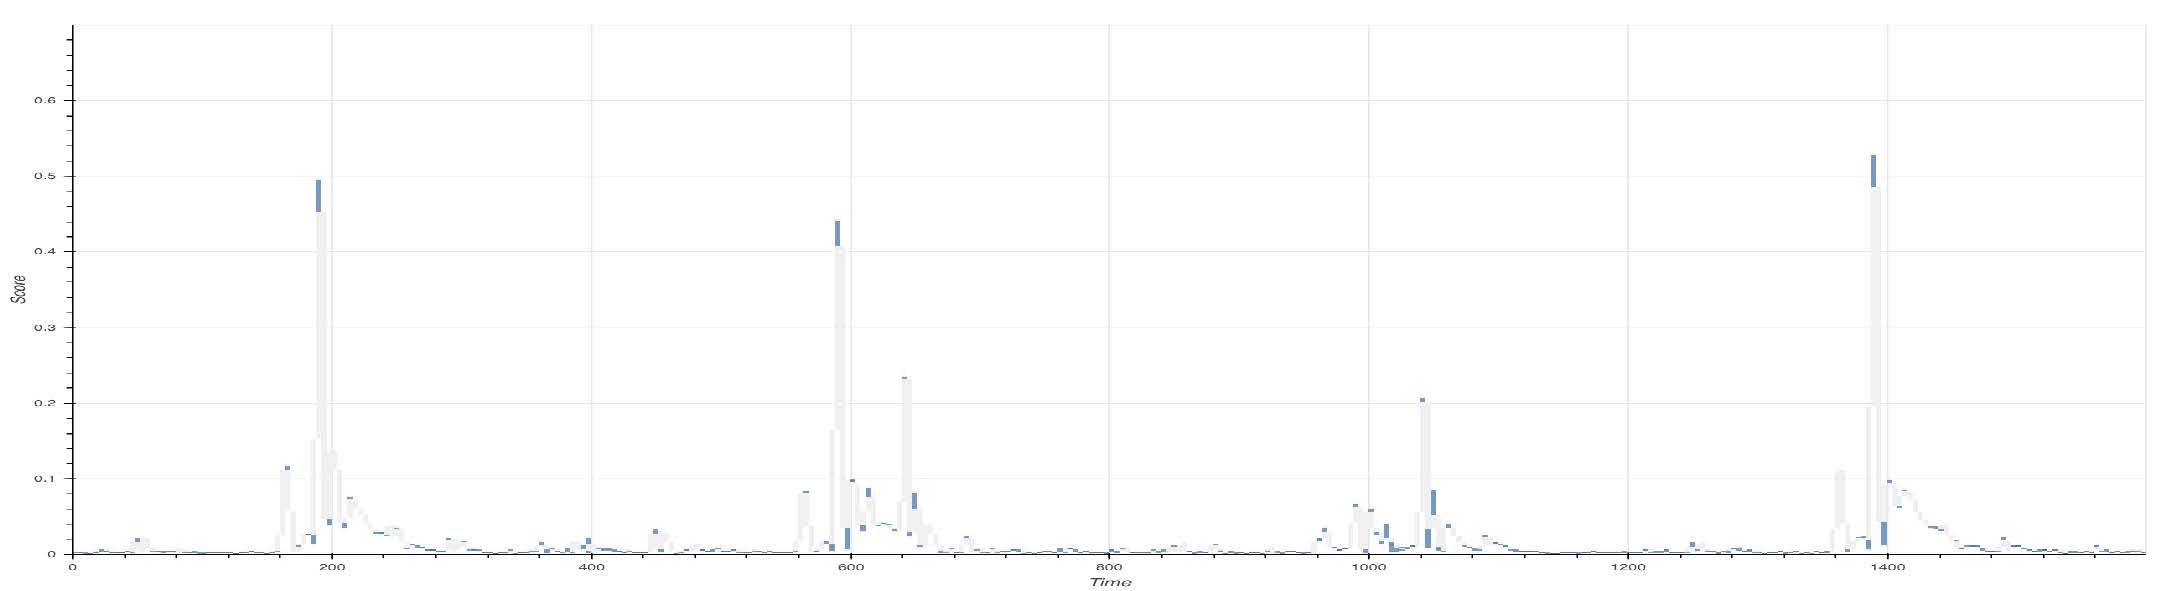
\includegraphics[width=\textwidth]{titansnr0123}
%			\caption{$\tilde \nonce_i\in\{0,1,2,3\}$}
%			\label{fig:titansnr0123}
%		\end{subfigure}%
%		\\% line break
%		\begin{subfigure}[b]{\textwidth}
%			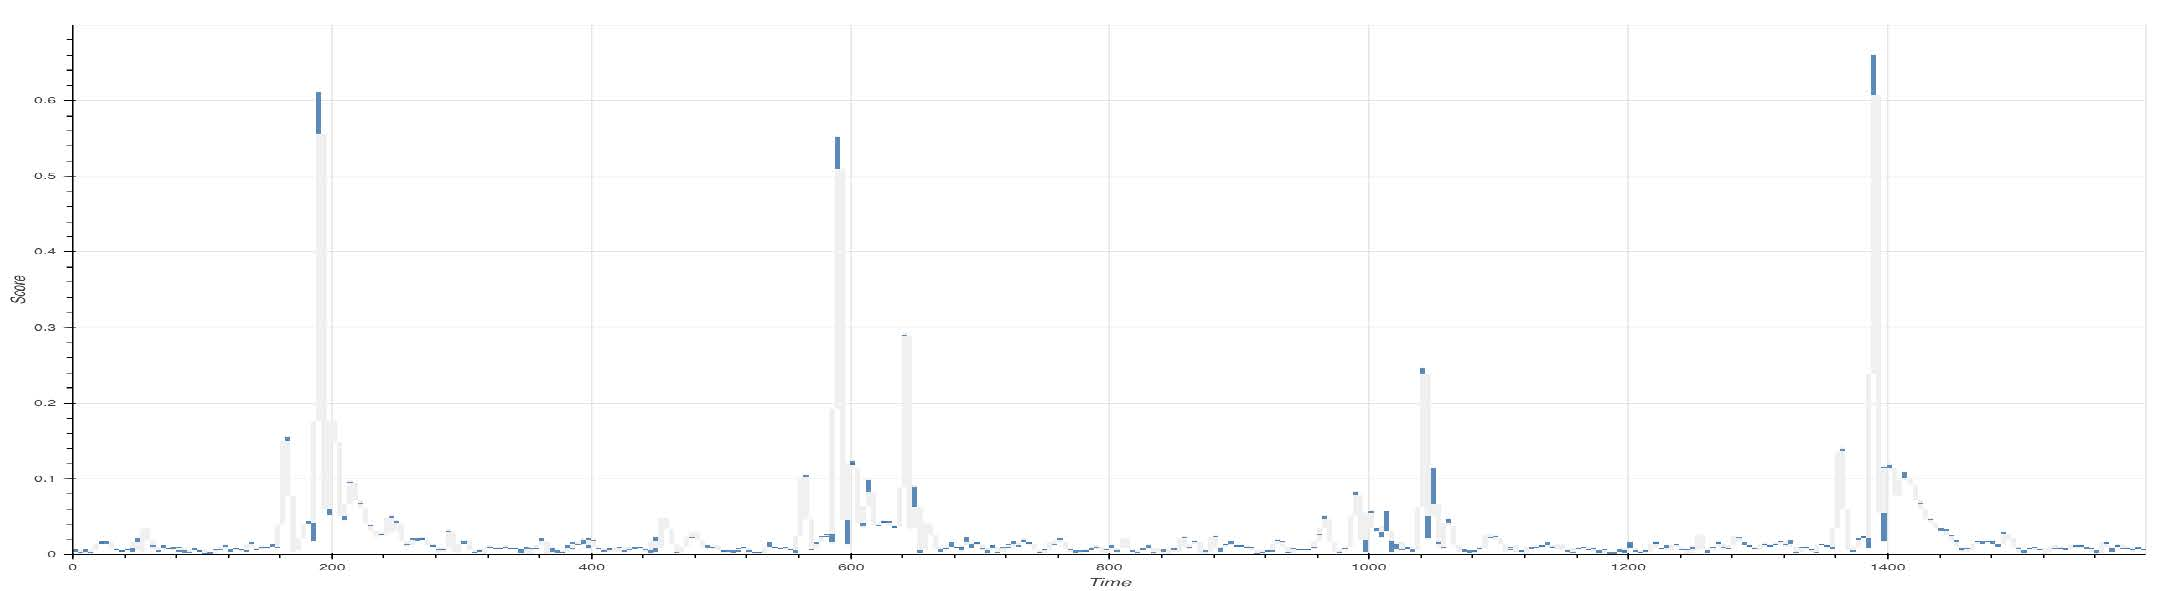
\includegraphics[width=\textwidth]{titansnr123}
%			\caption{$\tilde \nonce_i\in\{1,2,3\}$}
%			\label{fig:titansnr123}
%		\end{subfigure}
%		\bicaption{\enspace 信噪比结果}{\enspace SNR Results}
%		\label{fig:titansnr}
%	\end{figure}
%	
%	\algorithmref{alg:signscalar}只考虑了时间泄漏的防护。即使智能卡签名操作的数乘实现与\algorithmref{alg:signscalar}一致,也存在敏感数据泄漏的情况。Roche等\citep{Roche21}以\algorithmref{alg:signscalar}中的$\tilde \nonce_i$作为敏感中间值,对对齐后的电磁迹进行信噪比分析,实验结果如\figureref{fig:titansnr0123}所示。四类敏感中间值所计算出的SNR最大值为0.53。
%	
%	在\algorithmref{alg:signscalar}中$\tilde \multiplier_i\equiv \tilde\nonce_i$,当$\tilde \nonce_i=0$,虚拟的点加法$S+G_{\leakedmultiplier_i}$的被加数和加数实际上可以是任意两个椭圆曲线$E$上的点。Roche等\citep{Roche21}排除了敏感中间值$\tilde \nonce_i=0$时的能量迹重新计算SNR,实验结果如\figureref{fig:titansnr123}所示。三类敏感中间值所计算出的SNR最大值为0.65,相对于之前的信噪比有所提高,这说明对于$\tilde \nonce_i=0$这一类的点加法的电磁迹噪声较大,\algorithmref{alg:signscalar}第8行$\leakedmultiplier_i:=\tilde \nonce_i$很可能是错误的。
%	
%	Roche等\citep{Roche21}通过聚类的方法,验证了这样的事实:$\tilde \nonce_i=0$时,有$\frac12$的概率执行$\leakedmultiplier_i:=1$,有$\frac14$的概率执行$\leakedmultiplier_i:=2$,有$\frac14$的概率执行$\leakedmultiplier_i:=3$。Roche等\citep{Roche21}据此提出了更接近真实情况的签名操作的数乘实现的猜想,如\algorithmref{alg:improvesignscalar}所示。其中$G_1=G,G_2=2^{129}\cdot G,G_3=\left(2^{129}+1 \right) \cdot G,G_4=2^{128}\cdot G$。
%	
%	\begin{algorithm}
%		\caption{改进后签名操作的数乘算法}\label{alg:improvesignscalar}
%		\begin{algorithmic}[1]
%			\Statex \textbf{输入:} $\left\{\tilde{\nonce}_0,\tilde{\nonce}_1,\dots,\tilde{\nonce}_i,\dots, \tilde{\nonce}_{128}\right\}$:一次性随机数$\nonce$的长度为129的编码形式
%			\Statex \textbf{输入:} $G_1,G_2,G_3,G_4$:预计算的椭圆曲线$E$上的点
%			\Statex \textbf{输出:} $\nonce\cdot G$:基点$G$与一次性随机数$\nonce$数乘的结果
%			\State $S:=G_1$
%			\For{$i=1,\dots , 128$}
%			\State $S:=2\cdot S$
%			\If {$\tilde \nonce_i>0$}
%			\State $\leakedmultiplier_i:=\tilde \nonce_i$
%			\State $S:=S+G_{\leakedmultiplier_i}$\Comment{$\leakedmultiplier_i$存在泄漏}
%			\Else
%			\State $\leakedmultiplier_i\stackrel{\$}\gets\{1,1,2,3\}$\Comment{引入随机数}
%			\State $Dummy:=S+G_{\leakedmultiplier_i}$\Comment{$\leakedmultiplier_i$存在泄漏}
%			\EndIf
%			\EndFor
%			\If {$\tilde \nonce_0=0$}
%			\State $S:=S-G_4$
%			\Else
%			\State $Dummy:=S-G_4$
%			\EndIf
%			\State \Return $S$
%		\end{algorithmic}
%	\end{algorithm}
	
%	\subsection{随机数部分泄漏的请况下基于格的对ECDSA的攻击}\label{subs:infoforlattice}
%	
%	有大量工作\citep{Howgrave-Graham01,Nguyen02,Nguyen03,Hlavac06,Brumley11,Mulder14,Benger14,Goudarzi16,Fan16,Ryan19,Jancar20,Moghimi20,Weiser20,Micheli20}研究了在随机数泄漏少量比特的情况下攻击ECDSA方案,它们的主要思想是利用签名中的随机数的泄漏构造扩展隐藏数问题\citep{Boneh96}的方程并使用格基规约求解。
%	
%	利用一次性随机数$\nonce$的泄漏求解私钥$\sk$不在本文研究范围内,因此只做大致描述。它求解私钥的流程如\figureref{fig:solver}所示,我们将利用随机数部分泄漏使用基于格的ECDSA攻击抽象为调用一个求解算法,使用$\mathcal S$表示求解算法。
%	
%	\begin{figure}[!htb]
%		\centering
%		\begin{tikzpicture}[node distance=20pt]
%			\node[draw, rounded corners,align=center]  (start)  {运算开始};
%			\node[draw, trapezium, trapezium left angle=70, trapezium right angle=110,below=of start,align=center](inputleak){输入:用于构造方程的签名及其泄漏};
%			\node[draw, below=of inputleak,align=center] (constructequ)  {构造方程};
%			\node[draw, below=of constructequ,align=center] (solve)  {使用格基规约算法求解};
%			\node[draw, below=of solve,align=center] (calcd)  {根据最短向量求解私钥$\hat \sk$};
%			\node[draw, diamond, aspect=2, below=of calcd,align=center]     (chkd)  {$\hat \sk\cdot G=\pk$?};
%			
%			\node[draw, trapezium, trapezium left angle=70, trapezium right angle=110,align=center]at ([xshift=-40pt,yshift=-35pt]chkd.south west)(success){输出:"求解成功",$\sk=\hat \sk$};
%			\node[draw, trapezium, trapezium left angle=70, trapezium right angle=110,align=center]at ([xshift=40pt,yshift=-35pt]chkd.south east)(fail){输出:"求解失败"};
%			\node[draw, rounded corners, below=50pt of chkd,align=center]  (end) {运算结束};
%			
%			\draw[->] (chkd) -|node[midway,very near start,above] {是} (success);
%			\draw[->] (chkd) -|node[midway,very near start,above] {否} (fail);
%			
%			\draw[->] (success) |- (end);
%			\draw[->] (fail) |- (end);
%			\graph{
%				(start)->(inputleak)->(constructequ)->(solve)->(calcd) -> (chkd);
%			};
%		\end{tikzpicture}
%		\bicaption{\enspace 利用随机数部分泄漏使用基于格的ECDSA攻击流程图}{\enspace Flowchart of Lattice-based ECDSA Attacks with Partial Knowledge of the Nonces}
%		\label{fig:solver}	
%	\end{figure}
%	
%	$\mathcal S$是多项式时间复杂度的近似算法。只有构造方程签名中的的随机数泄漏需要同时满足三个限制时,$\mathcal S$才有较大可能在可接受的时间内求解出实际私钥$\sk$。三个限制如下所示。
%	
%	\begin{enumerate}
%		\item 用于构造方程的签名中的随机数泄漏需要可利用;
%		\item 用于构造方程的签名中的随机数泄漏需要足够多;
%		\item 用于构造方程的签名中的随机数泄漏的准确率是100\%。
%	\end{enumerate}
%	
%	本研究所使用的求解算法$\mathcal S$记为$S$。$S$求解时间约为400s。
%	
%	对于$S$,“可利用”指的是,恢复了\textbf{至少4个连续比特}签名中的一次性随机数$\nonce$泄漏以保证求解速度。如果使用没有4个连续比特随机数泄漏的签名构造方程,泄漏利用难度会增大,为了保证求解的正确性需要使用相对更多的签名,这会增加方程的维度从而增加求解时间。
%	
%	对于$S$,“足够多”指的是,需要\textbf{总共300比特}随机数泄漏的签名以构造正定或超定的方程,即需要$300\div 4=75$条有“可利用”随机数泄漏的签名。如果没有足够多的签名,那么构造的方程会欠定,这使得解空间变得非常大,无法求解实际私钥$d$。
%	
%	$S$对泄漏的准确率也有严格要求。这是因为一旦构造方程的泄漏存在错误(侧信道分析恢复的数据与实际数据不一致),那么方程会错误,求解出的私钥与实际私钥$\sk$一定不符。
	\section{本章小结}
	本章介绍了开展针对一类具有ECDSA实现的双界面商用智能卡的侧信道分析方法研究所需的背景知识,主要包括侧信道分析、数据增强、模拟退火和椭圆曲线数字签名算法。本章介绍的知识为读者提供论文所涉及领域的背景和上下文信息,帮助读者理解论文的主要观点和结果。
}
\chapter{面向基于深度学习侧信道分析的通用数据增强方法}\label{chap:search1}{
	
	%深度学习技术在侧信道攻击领域中得到了诸多应用,但样本数量不足的情况在实际中经常出现,这严重制约深度神经网络训练效果,甚至会直接影响攻击性能。因此,探讨样本数量有限情况下的数据增强方法,并讨论其对提升基于深度学习的侧信道攻击效果的实际影响,具有重要的现实意义。
	在深度学习的训练阶段对训练数据集进行数据增强可以使训练出的模型更准确,进而降低DL-SCA\chenggongtiaoshu 。然而,当前已有数据增强方法的参数选取通常高度依赖专家知识,且只适合对特定算法实现数据集进行数据增强。因此,构造一个适用于多种算法实现数据集的通用数据增强方法、自适应地选取数据增强参数,具有重要现实意义。
	
	本文选取了不同的AES实现作为分析目标,从数据增强的角度出发,研究减小成功实施DL-SCA所使用的能量迹条数的具有通用性的方法。分析目标包括无防护AES硬件实现、无防护AES软件实现、掩码(和随机延迟)防护AES软件实现以及随机延迟防护AES软件实现,这些实现对应的数据集分别为AES\_HD、DPA v4、ASCADf(N=0/N=50/N=100)、AES\_RD,他们都是侧信道领域权威公开数据集。本文提出了一种通用数据增强方法,其核心思想是采用模拟退火机制依据反馈信号自适应地选择数据增强策略参数。该方法主要由三个核心组件构成:采用模拟退火机制的主控制器、采用组合式数据增强机制的数据增强单元以及提供侧信道攻击代价反馈信号的攻击评估单元。以无防护软件和硬件AES实现、随机延迟和掩码防护AES软件实现为分析目标,在相应的本领域公开数据集上,开展了深度学习侧信道攻击实验对比研究,验证了本文所提出通用数据增强方法的有效性。具体地,在AES\_HD、DPA v4、ASCADf(N=0/N=50/N=100)三种数据集五个场景下,与未采用数据增强方法的DL-SCA效果相比,\chenggongtiaoshu 分别降低21\%、25\%、24\%、48\%以及5\%。在AES\_HD、DPA v4、ASCADf(N=0/N=50)三种数据集四个场景中,与采用其他数据增强方法的DL-SCA效果相比,\chenggongtiaoshu 分别降低22\%、40\%、10\%以及30\%。
	
	{\color{\xchange}
	
	\secref{sec:framework}对通用数据增强方法进行概念上的介绍,\secref{sec:intoreal}详细说明在AES实现上进行实验时通用数据增强方法这一概念的实例化结果,\secref{sec:realexp}汇报了采用通用数据增强方法DL-SCA技术效果。
	}
	
	\section{通用数据增强方法框架}\label{sec:framework}
	应用通用数据增强方法的侧信道分析框架如\figureref{fig:myframe}所示。该框架用于搜索最佳数据增强策略参数,其设计受到AutoAugment\citep{Cubuk19}的启发,它包含自适应数据增强方法、深度学习模型(见\subsref{subs:conceptdlsca})以及对应数据集三部分。其中,本研究提出的通用数据增强方法包含三个核心组件:主控制器(见\subsref{subs:conceptcontroller})、数据增强单元(见\subsref{subs:conceptcda})以及攻击评估单元(见\subsref{subs:concepteva}),其核心思想是采用模拟退火机制依据反馈信号自适应地调整数据增强策略参数。
	
	\begin{figure}[!h]
		\centering
		\begin{tikzpicture}[node distance=45pt, auto]
		% 定义节点样式
			\tikzstyle{reg} = [rectangle, draw,text centered]
			\tikzstyle{block} = [draw, rounded corners,align=center]
			\tikzstyle{data} = [draw, trapezium, trapezium left angle=70, trapezium right angle=110,align=center]
			%\tikzstyle{arrow} = [thick,->,>=stealth]
			
			%绘制节点
			\node [block,minimum width=200pt] (controller) {主控制器};
			\node [block,below of=controller, xshift=70pt](cda){数据增强单元};
			\node [block,below of=controller, xshift=-70pt](eva){攻击评估单元};
			\node [block,below=90pt of controller,minimum width=150pt](dlsca){深度学习模型};
			\node [data,below of=dlsca] (dataset){数据集};
			
			\draw [dashed] ([xshift=-25pt,yshift=10pt]controller.north west) rectangle ([xshift=25pt,yshift=-69pt]controller.north east) node [midway, yshift=5mm, above] {};
			\node at ([xshift=0,yshift=30pt]controller.north west)[anchor=north west]{通用数据增强方法};
			%		\path let \p1=(dataset.south west), \p2=(dataset.north west), \p3=(dataset.north east), \p4=(dataset.south east) in
			%		coordinate (A) at (\p1) 
			%		coordinate (B) at (\p2)
			%		coordinate (C) at (\p3)
			%		coordinate (D) at (\p4);
			
			
			\coordinate (controllersouth) at ($(controller.south)$);
			\coordinate (evanorth) at ($(eva.north)$);
			\coordinate (cdanorth) at ($(cda.north)$);
			\coordinate (evaend) at ($(eva.south)+(-20pt,0)$);
			\coordinate (evaend2) at ($(eva.south)+(+5pt,0)$);
			\coordinate (cdaend) at ($(cda.south)+(+20pt,0)$);
			\coordinate (cdastart) at ($(cda.south)+(-5pt,0)$);
			\coordinate (dlscanorth) at ($(dlsca.north)$);
			
			
			\draw[->] (dataset) -|node[pos=0.4,below] {算法输入、输出} (evaend);
			\draw[->] (dataset) -|node[pos=0.3,above] {验证标签} (evaend);
			\draw[->] (dataset) -|node[pos=0.3,below] {训练数据} (cdaend);
			\draw[->] (dataset) -|node[pos=0.3,above] {训练标签} (cdaend);
			
			\draw[->] (cdastart) --node[pos=0.3,left] {数据增强后} (cdastart|-dlscanorth);
			\draw[->] (cdastart) --node[pos=0.7,left] {的训练集} (cdastart|-dlscanorth);
			\draw[->] (evaend2|-dlscanorth) --node[pos=0.7,right] {验证数据} (evaend2);
			\draw[->] (evaend2|-dlscanorth) --node[pos=0.3,right] {预测结果} (evaend2);
			\graph{
				(evanorth)->["攻击代价"](evanorth|-controllersouth);
				(cdanorth|-controllersouth)->["数据增强策略参数" left](cdanorth);
				(dataset)->["验证数据"](dlsca);
				%(cdastart)->(cdastart|-dlscanorth);
				%(evaend2|-dlscanorth)->(evaend2);
			};
		\end{tikzpicture}
		\bicaption{\enspace 基于通用数据增强方法的侧信道分析框架概览}{\enspace Overview of the framework based on the general data augmentation method}
		\label{fig:myframe}
	\end{figure}
	{\color{\dupc}
			
	通过\figureref{fig:myframe}所示的攻击框架,我们将侧信道领域寻找最佳数据增强策略的问题转化为一个搜索问题。\figureref{fig:myframe}中各个部分与搜索问题的映射关系具体如下。
	
	首先,主控制器扮演着搜索问题中方案决策者角色,负责提供优化方向和指导。它依据反馈的攻击代价信号来不断调整并更新数据增强策略参数,提高侧信道分析技术效果。
	
	其次,数据增强单元充当着搜索问题中命令解析者角色,负责解析和实施主控制器给出的数据增强策略。它依据数据增强策略参数,对原始训练集进行数据增强,并输出数据增强后的训练集。
	
	随后,深度学习模型对应于搜索问题中的任务执行者角色,利用数据增强单元处理后的训练集进行训练,并通过验证集对正确密钥进行预测,得出正确密钥的预测结果和真实结果。它是整个框架中负责执行具体攻击任务和评估攻击效果的部分。
	
	最后,攻击评估单元对应于搜索问题中的评估者角色,用于计算攻击代价并反馈给主控制器。它利用攻击代价的计算公式,结合深度学习模型的预测结果和真实结果,将侧信道分析结果转化为主控制器所需要的攻击代价反馈信号。
	}
	\subsection{主控制器}\label{subs:conceptcontroller}
	如果将数据增强策略参数视为深度学习模型的某种超参数,那么主控制器的功能就是根据反馈信号自动地筛选超参数,以取代需要依赖大量专家知识的人工选择方法。
	
	{\color{\dupc}
		
		我们使用模拟退火机制构建主控制器。模拟退火是一种高效的启发式搜索算法,它具有良好的全局搜索能力。我们从多种自适应数据增强方法中选择模拟退火机制作为主控制器的原因如下。 
		
		首先,在自适应数据增强方法中,搜索算法的反馈信号灵活性高,可以自定义。自适应数据增强是指使用强化学习、元学习或搜索算法,自动地寻找最优数据增强策略的一类方法。搜索算法可以使用任何自定义的反馈信号,可以将适用于侧信道分析的攻击代价作为反馈信号。而其他的自适应数据增强方法如强化学习、元学习等则通常将准确率作为反馈信号,而准确率只能为测试数据集中的每个样本提供独立的标签预测信息。实际攻击中不同能量迹对应的密钥值一般相同,标签不是互相独立的,因此准确率作为侧信道分析评估指标时效果不佳\citep{Picek19}。
		
		其次,在搜索算法中,启发式搜索算法占用资源少,能在大规模复杂问题中进行高效搜索。搜索算法可以分为网格搜索、随机搜索和启发式搜索算法。启发式搜索算法与网格搜索相比,有更好的全局搜索能力,无需对参数离散化处理,从而避免了维度灾难,资源使用更少;启发式搜索算法与随机搜索算法相比,效率较高。
		
		最后,在启发式搜索算法中,模拟退火具有效率高和适用性强的特点。启发式算法包括遗传算法、粒子群算法、蚁群算法、禁忌搜索和模拟退火等多种算法。在时间效率方面,模拟退火算法的优势在于每次迭代仅需要计算代价和部分随机数,相较于涉及复杂的操作和运算的遗传算法、粒子群算法和蚁群算法,效率更高。在适用性方面,禁忌搜索产生新解的方式复杂,难以依据数据增强策略参数与攻击验证的结果的对应关系构造禁忌表。
		
		综上所述,鉴于反馈信号灵活性高、资源占用率少、效率高以及适用性强等技术特点,我们选择模拟退火算法作为通用数据增强方法主控制器。
	}
	\subsection{数据增强单元}\label{subs:conceptcda}
	
	数据增强单元的作用是根据数据增强策略参数训练集进行数据增强,数据增强后的训练集会被用于深度学习模型的训练。数据增强单元与深度学习的训练阶段的耦合关系如\figureref{fig:mycdaanddlsca}所示,它相比于\figureref{fig:dltrainphase}表示的深度学习的训练阶段,增加了数据增强单元。通过对数据进行扩充,模型能够学习到更多的变化模式和特征,从而提高其泛化能力,使其在未知数据(如验证集、测试集)上表现更好。
	
	\begin{figure}[!h]
		\centering
		\begin{tikzpicture}[node distance=45pt, auto]
			% 定义节点样式
			\tikzstyle{reg} = [rectangle, draw,text centered]
			\tikzstyle{block} = [draw, rounded corners,align=center]
			\tikzstyle{data} = [draw, trapezium, trapezium left angle=70, trapezium right angle=110,align=center]
			\tikzstyle{arrow} = [thick,->,>=stealth]
			\tikzstyle{rarrow} = [thick,<-,>=stealth]
			
			% 绘制节点
			\node [reg] (parareg) {参数寄存器};
			\node [block,below of =parareg] (trained) {深度神经网络};
			\node [reg, left=70pt of trained] (hyperparareg) {超参数寄存器};
			\node [block, right=120pt of trained] (valacc) {机器学习\\指标计算器};
			\node [block, below of=trained] (cda){数据增强单元};
			\node [data, below of=cda] (dataset) {数据集};
			\node [block,above of =parareg] (paracalc) {反向传播算法\\梯度下降算法};
			
			%\node [block, below of=valacc, xshift=2cm] (testacc) {测试集准确率计算器};
			
			% 绘制箭头
			\draw [arrow] (cda) -- node[right] {数据增强后的训练数据} (trained);
			\draw [arrow] (cda) -| node[pos=0.25,below] {数据增强后的训练标签} (valacc);
			%\draw [arrow] (dataset) -- node[above] {测试数据} (pretrained);
			\draw [arrow] (trained) -- node[above] {训练数据的预测结果} (valacc);
			\draw [arrow] (hyperparareg) -- node[above]{网络超参数}(trained);
			\draw [arrow] (parareg) -- node[right]{神经元参数}(trained);
			\draw [arrow] (valacc)|- node[pos=0.75, above] {训练交叉熵}(paracalc);
			\draw [arrow] (paracalc)--node[pos=0.5, right] {调整后的神经元参数}(parareg);
			\draw [arrow] (dataset) --node[right]{训练集}(cda);
			\draw [arrow] (hyperparareg)|- node[pos=0.75, above] {数据增强策略参数}(cda);
			%\draw [rarrow] (cda) --node[midway, below] {数据增强策略参数} ++(180:120pt);
		\end{tikzpicture}
		\bicaption{\enspace 攻击AES的引入数据增强单元的深度学习训练阶段}{\enspace DL training process with data augmentation unit for SCA on AES}
		\label{fig:mycdaanddlsca}
	\end{figure}
%	\begin{algorithm}
%		\caption{位移变换 shift\_deformation}\label{alg:shift}
%		\begin{algorithmic}[1]
%			\Statex \textbf{输入:} 能量迹$\vec x=\begin{bmatrix}
%			x_1&x_2&\cdots&x_{M-1}
%			\end{bmatrix}$,最大位移幅度$m_1, 0\le m_1<M$
%			\Statex \textbf{输出:}能量迹$\vec y=\begin{bmatrix}
%			y_1&y_2&\cdots&y_{M-1}
%			\end{bmatrix}$
%			\State $s\gets\{-m_1,-m_1+1,-m_1+2,\dots,m_1-1,m_1\}$
%			\For{$n := 0, \dots, M-1$}
%			\State $y_i:= x_{(i+s)\mod M}$
%			\EndFor
%		\end{algorithmic}
%	\end{algorithm}
%	
%	\begin{algorithm}
%		\caption{添加噪声 add\_noise}\label{alg:noise}
%		\begin{algorithmic}[1]
%			\Statex \textbf{输入:} 能量迹$\vec x=\begin{bmatrix}
%			x_1&x_2&\cdots&x_{M-1}
%			\end{bmatrix}$,噪声方差$m_2$
%			\Statex \textbf{输出:}能量迹$\vec y=\begin{bmatrix}
%			y_1&y_2&\cdots&y_{M-1}
%			\end{bmatrix}$
%			\For{$n := 0, \dots, M-1$}
%			\State $e_i\gets N(0,m_2)$
%			\State $y_i:= x_i+e_i$
%			\EndFor
%		\end{algorithmic}
%	\end{algorithm}
%	
%	\begin{algorithm}
%		\caption{合成少数类过采样法 SMOTE}\label{alg:smote}
%		\begin{algorithmic}[1]
%			\Statex \textbf{输入:} 能量迹$\vec x=\begin{bmatrix}
%			x_1&x_2&\cdots&x_{M-1}
%			\end{bmatrix},\vec y=\begin{bmatrix}
%			y_1&y_2&\cdots&y_{M-1}
%			\end{bmatrix}$,参数$m_3$
%			\Statex \textbf{输出:}能量迹$\vec z=\begin{bmatrix}
%			z_1&z_2&\cdots&z_{M-1}
%			\end{bmatrix}$
%			\State $\lambda\gets B(m_3,m_3)$
%			\For{$n := 0, \dots, M-1$}
%			\State $z_i:=(1-\lambda)x_i+\lambda y_i$
%			\EndFor
%		\end{algorithmic}
%	\end{algorithm}
	
	\subsection{侧信道分析中的深度学习模型}\label{subs:conceptdlsca}
	
	DL-SCA是结合深度学习技术的模板类侧信道分析。
	
	%深度学习分为三个阶段:训练阶段、验证阶段、测试阶段。训练阶段的主要目的是让模型学习从输入数据到输出预测的映射关系,以便模型能够在未见过的数据上进行准确的预测,。验证阶段的目的是评估模型在未见过的数据上的性能。测试阶段的目的是最终评估模型的性能。
	
	深度学习分为三个阶段:训练阶段、验证阶段和测试阶段。在训练阶段,我们使用训练集来调整神经网络的神经元参数,这是通过使用反向传播和梯度下降最小化交叉熵损失函数实现的,如\figureref{fig:dltrainphase}所示。这样,模型可以学习从输入数据到输出预测的映射关系,以便在未见过的数据上进行准确的预测。
	
	验证阶段的目的是绘制交叉熵和准确率曲线,以供肉眼判断超参数的合理性。通常情况下,我们会执行多次训练阶段,然后进行一次验证阶段。通过观察验证集上的性能表现,我们可以调整超参数,如学习率、正则化参数等,以提高模型的泛化能力和性能,如\figureref{fig:dlvalidationphase}所示。
	
	最终,当我们经过多次验证阶段确定了最佳的超参数设置之后,我们会进入测试阶段。测试数据集的目的是对经过训练和验证的模型进行最终评估,以获得模型在真实场景下的性能表现,如\figureref{fig:dltestphase}所示。测试阶段的结果可以提供对模型的客观评估,并帮助我们了解模型在实际应用中的表现。
	
	\begin{figure}[!htbp]
		\centering
		\begin{subfigure}[b]{\textwidth}
			{
				\small 
				\begin{tikzpicture}[node distance=45pt, auto]
					% 定义节点样式
					\tikzstyle{reg} = [rectangle, draw,text centered]
					\tikzstyle{block} = [draw, rounded corners,align=center]
					\tikzstyle{data} = [draw, trapezium, trapezium left angle=70, trapezium right angle=110,align=center]
					\tikzstyle{arrow} = [thick,->,>=stealth]
					
					% 绘制节点
					\node [reg] (hyperparareg) {超参数寄存器};
					\node [block,below of =hyperparareg] (trained) {深度神经网络};
					\node [block, right=100pt of trained] (valacc) {机器学习\\指标计算器};
					\node [reg, left=70pt of trained] (parareg) {参数寄存器};
					\node [data, below of=trained] (dataset) {数据集};
					\node [block,below of=dataset] (paracalc) {反向传播算法\\梯度下降算法};
					
					%\node [block, below of=valacc, xshift=2cm] (testacc) {测试集准确率计算器};
					
					% 绘制箭头
					\draw [arrow] (dataset) -- node[right] {训练数据} (trained);
					\draw [arrow] (dataset) -| node[pos=0.25,below] {训练标签} (valacc);
					%\draw [arrow] (dataset) -- node[above] {测试数据} (pretrained);
					\draw [arrow] (trained) -- node[above] {训练数据的预测结果} (valacc);
					\draw [arrow] (hyperparareg) -- node[right]{网络超参数}(trained);
					\draw [arrow] (parareg) -- node[above]{神经元参数}(trained);
					\draw [arrow] (valacc) --  ++(0:50pt) |- node[pos=0.75, above] {训练交叉熵}(paracalc);
					\draw [arrow] (paracalc)-|node[pos=0.25, above] {调整后的神经元参数}(parareg);
					%\draw [arrow] (valacc) --node[midway, below] {训练交叉熵} ++(0:100pt);
				\end{tikzpicture}
			}
			\caption{训练阶段}
			\label{fig:dltrainphase}
		\end{subfigure}%
		\\% line break
		\begin{subfigure}[b]{\textwidth}
			{
				\small
				\begin{tikzpicture}[node distance=45pt, auto]
					% 定义节点样式
					\tikzstyle{reg} = [rectangle, draw,text centered]
					\tikzstyle{block} = [draw, rounded corners,align=center]
					\tikzstyle{data} = [draw, trapezium, trapezium left angle=70, trapezium right angle=110,align=center]
					\tikzstyle{arrow} = [thick,->,>=stealth]
					
					% 绘制节点
					\node [reg] (hyperparareg) {超参数寄存器};
					\node [block,below of =hyperparareg] (trained) {深度神经网络};
					\node [block, right=100pt of trained] (valacc) {机器学习\\指标计算器};
					\node [reg, left=70pt of trained] (parareg) {参数寄存器};
					\node [data, below of=trained] (dataset) {数据集};
					\node [block,above of=valacc] (hyperparacalc) {肉眼观察};
					
					%\node [block, below of=valacc, xshift=2cm] (testacc) {测试集准确率计算器};
					
					% 绘制箭头
					\draw [arrow] (dataset) -- node[right] {验证数据} (trained);
					\draw [arrow] (dataset) -| node[pos=0.25,below] {验证标签} (valacc);
					%\draw [arrow] (dataset) -- node[above] {测试数据} (pretrained);
					\draw [arrow] (trained) -- node[above] {验证数据的预测结果} (valacc);
					\draw [arrow] (hyperparareg) -- node[right]{网络超参数}(trained);
					\draw [arrow] (parareg) -- node[above]{神经元参数}(trained);
					\draw [arrow] (valacc) -- node[left] {验证交叉熵曲线}(hyperparacalc);
					\draw [arrow] (valacc) -- node[right] {验证准确率曲线}(hyperparacalc);
					\draw [arrow] (hyperparacalc)--node[ above] {调整后的网络超参数}(hyperparareg);
					%\draw [arrow] (valacc) --node[midway, below] {训练交叉熵} ++(0:100pt);
				\end{tikzpicture}
			}
			\caption{验证阶段}
			\label{fig:dlvalidationphase}
		\end{subfigure}%
		\\% line break
		\begin{subfigure}[b]{\textwidth}
			{
				\small
				\begin{tikzpicture}[node distance=45pt, auto]
					% 定义节点样式
					\tikzstyle{reg} = [rectangle, draw,text centered]
					\tikzstyle{block} = [draw, rounded corners,align=center]
					\tikzstyle{data} = [draw, trapezium, trapezium left angle=70, trapezium right angle=110,align=center]
					\tikzstyle{arrow} = [thick,->,>=stealth]
					
					% 绘制节点
					\node [reg] (hyperparareg) {超参数寄存器};
					\node [block,below of =hyperparareg] (trained) {深度神经网络};
					\node [block, right=100pt of trained] (valacc) {机器学习\\指标计算器};
					\node [reg, left=70pt of trained] (parareg) {参数寄存器};
					\node [data, below of=trained] (dataset) {数据集};
					
					%\node [block, below of=valacc, xshift=2cm] (testacc) {测试集准确率计算器};
					
					% 绘制箭头
					\draw [arrow] (dataset) -- node[right] {测试数据} (trained);
					\draw [arrow] (dataset) -| node[pos=0.25,below] {测试标签} (valacc);
					%\draw [arrow] (dataset) -- node[above] {测试数据} (pretrained);
					\draw [arrow] (trained) -- node[above] {测试数据的预测结果} (valacc);
					\draw [arrow] (hyperparareg) -- node[right]{网络超参数}(trained);
					\draw [arrow] (parareg) -- node[above]{神经元参数}(trained);
					\draw [arrow] (valacc) --node[midway, above] {测试交叉熵} ++(0:100pt);
					\draw [arrow] (valacc) --node[midway, below] {测试准确率} ++(0:100pt);
				\end{tikzpicture}
			}
			\caption{测试阶段}
			\label{fig:dltestphase}
		\end{subfigure}%
		\bicaption{\enspace 深度学习训练过程}{\enspace DL training process}
		\label{fig:dlallphase}
	\end{figure}
	
	%在基于深度学习的侧信道攻击中,建模阶段可以对应于深度学习的训练和验证阶段,攻击阶段可以对应于深度学习的测试阶段。但是攻击阶段和测试阶段略有不同,\figureref{fig:dltestphase}和\figureref{fig:attackphase}分别展示了攻击阶段和测试阶段的示意图。从图中可以看到测试阶段直接依据标签和和标签预测结果直接计算准确率等指标,攻击阶段多了一个步骤,它需要依据标签计算算法密钥、组合多条迹的标签预测结果计算密钥预测值,最后通过算法密钥和密钥预测值计算成功率等侧信道攻击指标。
	
	总的来说,训练阶段用于调整神经网络的参数,验证阶段用于确定超参数的合理性,而测试阶段则是最终评估模型性能的阶段。在实际应用中,通常会进行多次训练和验证阶段,以找到最佳的超参数设置,然后进行一次测试阶段来得到最终的性能评估。
	
	在基于通用数据增强方法的框架中,深度学习的三个阶段需要进行相应改动以适配其它组件或适配侧信道分析需求。
	
	如果将数据增强策略参数视为深度学习模型的某种超参数,那么数据增强策略参数应该在验证阶段进行调整。调整的机制如\figureref{fig:mydlscaandetc}所示,它相比于\figureref{fig:dlvalidationphase}表示的深度学习的验证阶段,需要执行更多步骤才能调整超参数,这是为了使用侧信道分析相关的评估指标来指导超参数的修改,使得优化过程更为合理。需要注意的是,基于通用数据增强方法的框架不会改变预先设定的神经网络架构相关的超参数,寻找合适的网络架构并不属于本研究的内容。
	
	\begin{figure}[!h]
		\centering
		\begin{tikzpicture}[node distance=45pt, auto]
			% 定义节点样式
			\tikzstyle{reg} = [rectangle, draw,text centered]
			\tikzstyle{block} = [draw, rounded corners,align=center]
			\tikzstyle{data} = [draw, trapezium, trapezium left angle=70, trapezium right angle=110,align=center]
			\tikzstyle{arrow} = [thick,->,>=stealth]
			
			% 绘制节点
			\node [reg] (hyperparareg) {超参数寄存器};
			\node [block,below of =hyperparareg] (trained) {深度神经网络};
			\node [reg, left=70pt of trained] (parareg) {参数寄存器};
			\node [data, below of=trained] (dataset) {数据集};
			\node [block, right=100pt of dataset] (keypred) {密钥预测器};
			\node [block, below of =dataset] (keycalc) {密钥计算器};
			\node [block, below =50pt of keypred] (cmp) {侧信道分析\\指标计算器};
			\node [block, right=170pt of trained]  (hyperparacalc) {主控制器};
			
			%\node [block, below of=valacc, xshift=2cm] (testacc) {测试集准确率计算器};
			
			% 绘制箭头
			\draw [arrow] (dataset) -- node[right] {验证数据} (trained);
			\draw [arrow] (dataset) -- node[left] {验证标签(敏感中间值)} (keycalc);
			\draw [arrow] (dataset) -- node[pos=0.45,above] {算法输入、输出} (keypred);
			\draw [arrow] (dataset) -- ++(0:100pt) |- (keycalc);
			%\draw [arrow] (dataset) -- node[above] {测试数据} (pretrained);
			\draw [arrow] (trained) -| node[pos=0.3,above] {验证数据的标签预测结果} (keypred);
			\draw [arrow] (hyperparareg) -- node[right]{网络超参数}(trained);
			\draw [arrow] (parareg) -- node[above]{神经元参数}(trained);
			
			\draw [arrow] (keypred) -- node[right]{密钥预测值}(cmp);
			\draw [arrow] (keycalc) |- node[pos=0.7,below]{算法密钥}(cmp);
			\draw [arrow] (cmp) -|node[pos=0.3, below] {攻击代价} (hyperparacalc);
			\draw [arrow] (hyperparacalc)|-node[pos=0.7,above]{新的数据增强策略参数}(hyperparareg);
		\end{tikzpicture}
		\bicaption{\enspace 攻击AES的用于调整数据增强策略参数的深度学习验证阶段}{\enspace DL validation phase for updating DA parameters for SCA on AES}
		\label{fig:mydlscaandetc}
	\end{figure}
	
	
	%深度学习的训练阶段对应于模板类侧信道攻击中的建模阶段,深度学习的验证阶段不对应于模板类侧信道攻击中的任何一个阶段,深度学习的测试阶段类似于模板类侧信道攻击中的攻击阶段\footnote{实际上略有不同,模板类侧信道攻击中的攻击阶段,除了需要对每条迹的标签进行预测(这类似于深度学习的测试阶段),还可以选取多条迹的预测结果进行组合才能最终计算出密钥估计值。}。
	\subsection{攻击评估单元}\label{subs:concepteva}
	攻击评估单元的功能是量化并输出攻击代价。\figureref{fig:mydlscaandetc}中的密钥计算器、密钥预测器、侧信道分析指标计算器组合成了攻击评估单元。如何根据验证数据的标签预测结果计算密钥预测值、如何根据验证标签计算算法密钥、计算哪方面的侧信道分析评估指标作为攻击代价反馈给主控制器,这些都要根据具体算法实现进行单独的分析。
	
	攻击评估单元如果使用不合理的侧信道分析评估指标作为攻击代价反馈给主控制器,它会使得主控制器依据不准确的指标进行参数更新,进而导致主控制器无法优化数据增强策略参数。
	\section{通用数据增强方法在AES算法实现分析中的应用}\label{sec:intoreal}
	\subsection{AES算法实现数据集}
	
	本研究使用了四个侧信道领域广泛使用的公开数据集共六种实际场景,这些数据集涵盖侧信道分析场景的主要类型。第一个数据集DPA v4所对应的算法实现无任何防护,并且噪声水平低。这个数据集代表了理想的攻击目标,难度最低,因此它能评价攻击技术最佳行为\footnote{因为它难度最低,所以对于同一个攻击技术,对于这个数据集的攻击结果,从理论上来说会比其他数据集的攻击结果更优。}。第二个数据集AES\_HD所对应的算法实现同样不包含任何防护措施,但是它有较高的噪声水平。这个数据集为模板类侧信道分析带来一定难度,因为高水平噪声使得类之间的界限变得模糊不清。第三个数据集AES\_RD所对应的算法实现使用了随机延迟防护措施。随机延迟是一种实际应用中很常见的防护措施,因此该数据集代表很常见的现实攻击场景。第四个数据集ASCADf对应的算法实现使用了掩码防护措施。掩码是一种可证明安全的防护措施,因此它是一种广泛使用的抵御侧信道分析的防护措施。ASCADf可以依据引入的随机延迟的程度进一步划分为三种实际场景,更大范围的随机延迟程度对应更高的攻击难度。
	
	\subsubsection{DPA v4数据集}
	
	这个数据集对应了掩码防护的AES软件实现\footnote{数据来源:第四届DPA Contest大赛 \href{http://www.dpacontest.org/v4}{http://www.dpacontest.org/v4}。}。Moradi等\citep{Moradi14}发现这个数据存在一阶泄漏,我们直接认为掩码是已知的,这时候掩码防护措施退化为无防护场景。因为算法实现的平台是ATMEL AVR-163微控制器,因此我们选择软件实现泄漏最多的第一轮字节替换操作作为攻击目标。以攻击主密钥第0字节为例,数据集中的标签计算方式如\equationref{eq:dpav4model}所示。
	
	\begin{equation}\label{eq:dpav4model}
		label=\overbrace{\mathrm{Sbox}}^{\mbox{已知}}[\overbrace{p_0}^{\mbox{已知}}\oplus k_0]\oplus \overbrace{mask_0}^{\mbox{已知}}
	\end{equation}
	
	\noindent 其中$p_0$表示明文第0字节的值,$k_0$表示主密钥第0字节的值,$mask_0$表示算法第1轮掩码第0字节的值。
	
	\subsubsection{AES\_HD数据集}
	这个数据集对应了无防护的AES硬件\footnote{数据来源:AES\_HD\_Dataset \href{https://github.com/AESHD/AES\_HD\_Dataset}{https://github.com/AESHD/AES\_HD\_Dataset}。}实现。AES-128核心部件使用VHDL编写的,它采用多轮的架构,每次加密需要11个时钟周期。该设计在Xilinx Virtex-5 FPGA的SASEBO GII评估板上实现。攻击者将高灵敏度的电磁探针放置在电源线的去耦合电容附近,使用Teledyne LeCroy Waverunner 610zi示波器采样,从而获得包含信息泄漏的电磁迹。硬件实现中寄存器写通常存在比较明显的泄漏,我们选择最后一轮(第10轮)轮密钥的第7字节选为攻击目标,数据集中的标签计算方式如\equationref{eq:aeshdmodel}所示。采集的电磁迹含有4000个采样点。本研究使用其中的5000条。
	
	\begin{equation}
		\begin{cases}
			reg_{round9}=y\\
			reg_{round10}=c_{7}\\
			c_{11}=\mathrm{Sbox}[y\oplus k_7]\\
			label =\underbrace{\overbrace{\mathrm{Sbox}^{-1}}^{\mbox{已知}}[\overbrace{c_{11}}^{\mbox{已知}}\oplus k_{7}]}_{reg_{round9}}\oplus \underbrace{\overbrace{c_{7}}^{\mbox{已知}}}_{reg_{round10}}
		\end{cases}\label{eq:aeshdmodel}
	\end{equation}
	
	\noindent 其中,$reg_{round9},reg_{round10}$分别表示硬件代码中一个寄存器\footnote{该寄存器寄存的值在第10个周期的上升沿时发生变化,电磁场强度与这个变化有一定关系,因此可以通过侧信道分析恢复每一次的变化值。又因为这个变化值和密钥有关,所以可以进一步恢复密钥。}在算法第9、10个周期的所寄存的值,$c_7,c_{11}$分别表示算法输出的第7、11字节,$k_7$表示第10轮轮密钥的第7字节。攻击者令算法执行1000000次,每次随机明文,最终采集到了1000000条采样点个数为1250的电磁迹。本研究只使用其中的75000条。
	
	\subsubsection{AES\_RD数据集}
	这个数据集对应了使用了防护措施的AES算法,它在一个使用8比特AVR微控制器的ATmega16智能卡上实现\footnote{数据来源:Trace sets with random delays \href{https://github.com/ikizhvatov/randomdelays-traces}{https://github.com/ikizhvatov/randomdelays-traces}。}。算法使用的防护措施是Coron等\citep{Coron09}所描述的随机延迟。在加密算法的正常运行中添加随机延迟会使得重要的信息泄漏特征错位,进而增加攻击的难度。我们还是选定第一轮字节替换操作作为攻击目标。以攻击主密钥第0字节为例,数据集中的标签计算方式如\equationref{eq:aesrdmodel}所示。
	
	\begin{equation}\label{eq:aesrdmodel}
		label=\overbrace{\mathrm{Sbox}}^{\mbox{已知}}[\overbrace{p_0}^{\mbox{已知}}\oplus k_0]
	\end{equation}
	
	数据集包含50000条有3500个采样点的能量迹或电磁迹,本研究使用该数据集所有的能量迹或电磁迹。
	\subsubsection{ASCADf数据集}
	Benadjila等\citep{Benadjila20}在一个使用8比特AVR微控制器的ATmega16智能卡上实现了有掩码防护措施的AES-128算法,并采集智能卡加密过程中的电磁辐射生成了ASCAD数据集\footnote{数据来源:ASCAD \href{https://github.com/ANSSI-FR/ASCAD}{https://github.com/ANSSI-FR/ASCAD}}。我们还是选定第一轮字节替换操作作为攻击目标。以攻击主密钥第2字节\footnote{AES算法不同字节密钥的攻击难度可能不同。在Benadjila等的研究中重点汇报了对主密钥第三字节进行攻击的结果,我们也选择第三字节作为攻击目标可以保证比较是公平的。}为例,数据集中的标签计算方式如\equationref{eq:ascadbadmodel}所示。但是在建模阶段,$mask_2$是无法知道的,这会导致无法计算标签。为了解决这个问题,我们直接舍去$mask_2$,这样就可以计算出标签\footnote{对于一阶掩码实现,信息泄漏与标签之间不再存在某种线性关系。但是深度神经网络有可能学习到信息泄漏与标签之间的非线性关系,进而完成DL-SCA。},如\equationref{eq:ascadmodel}所示。
	
	\begin{equation}\label{eq:ascadbadmodel}
		label=\overbrace{\mathrm{Sbox}}^{\mbox{已知}}[\overbrace{p_2}^{\mbox{已知}}\oplus k_2]\oplus mask_2
	\end{equation}
	
	\begin{equation}\label{eq:ascadmodel}
		label=\overbrace{\mathrm{Sbox}}^{\mbox{已知}}[\overbrace{p_2}^{\mbox{已知}}\oplus k_2]
	\end{equation}
	
	ASCAD数据集主要分成两个部分:一个部分使用固定的密钥设置(记为ASCADf),另一个部分使用随机的密钥设置(记为ASCADr)。本文只使用ASCADf。ADCADf数据集包含60000条电磁迹。本研究使用该数据集所有的迹,并从每条迹中过滤出包含敏感信息泄漏的700个采样点。
	
	除此之外,Benadjila等向数据集中添加了使用脚本模拟的随机延迟,以测试神经网络抗抖动的能力。根据随机延迟程度不同,ASCADf数据集可以进一步分为三个:ASCADf(N=0)、ASCADf(N=50)以及ASCADf(N=100),它们分别对应于延迟最多0、50以及100个采样点的场景。
	
	\subsubsection{数据处理}
	
	进行DL-SCA时,我们需要进一步将数据集划分为互不重叠的三个部分:训练集、验证集\footnote{如果验证集与测试集有重叠,模型在验证阶段可能会因为对验证集的过拟合,导致对模型性能的估计过于乐观。}、测试集。具体划分比例如\tableref{tab:partition}所示。我们使用k-fold交叉验证的思想评估模型性能。以DPA v4数据集为例,在一次实验中,我们首先随机地将数据集划分为大小为4500和500的两部分(分别记为A和B),接着独立地进行五次训练过程。在每次训练过程开始时,我们随机地将A进一步划分为大小为4000和500的两部分(分别记为A$_1$和A$_2$)。在这之后我们使用A$_1$作为训练集,A$_2$作为验证集,B作为测试集,进行一次训练过程。每次执行训练过程后,对测试集每个样本预测的概率向量都会被记录下来。%在每次训练过程的阶段之后,独立计算100次密钥估计值并汇总评价指标的平均值。
	\begin{table}[!h]
		\bicaption{\enspace 数据集划分方式}{\enspace Partition of training/ test set for all open datasets}
		\label{tab:partition}
		\centering
		%\footnotesize% fontsize
		%\setlength{\tabcolsep}{4pt}% column separation
		%\renewcommand{\arraystretch}{1.2}%row space 
		\begin{tabular}{c|ccc}
			\hline
			数据集名称&训练样本数量&验证训练样本数量&测试训练样本数量\\
			\hline
			DPA v4    &4000 &500 &500\\
			AES\_HD   &45000&5000&25000\\
			AES\_RD   &20000&5000&25000\\
			ASCADf(N=0)&45000&5000&10000\\
			ASCADf(N=50)&45000&5000&10000\\
			ASCADf(N=100)&45000&5000&10000\\
			\hline
		\end{tabular}
	\end{table}
	\subsection{实验设置}
	\subsubsection{主控制器设置}\label{subss:controllersettings}
	选定了使用模拟退火机制实现主控制器后,主控制器的实现如\algorithmref{alg:saincontroller}所示。可以看到它已经将\algorithmref{alg:sa}中的解和能量函数实例化。\algorithmref{alg:sa}中的解这一概念和组合式数据增强中的数据增强策略参数对应。数据增强单元依据数据增强策略参数进行数据增强、深度学习模型使用数据增强后的训练集训练和使用验证集进行预测、攻击评估单元反馈攻击代价,这整个流程可以抽象为一个函数$cost(\cdot)$,它输入数据增强策略参数,输出攻击代价。调用一次$cost(\cdot)$对应于调用一次\algorithmref{alg:sa}中的能量函数。
	
	\begin{breakablealgorithm}
		\caption{主控制器的模拟退火实现}\label{alg:saincontroller}
		\begin{algorithmic}[1]
			\Statex \textbf{输入:} $state=(p_{ro},m_{ro},p_{an},m_{an},p_{os},m_{os})$:初始数据增强策略参数
			\Statex \textbf{输入:} $inittemp$:初始温度
			\Statex \textbf{输入:} $\gamma\in(0,1)$:退火速度
			\Statex \textbf{输入:} $n$:迭代次数
			\Statex \textbf{输入:} $Energy(\cdot)=cost(\cdot)$攻击代价计算函数
			\Statex \textbf{输出:} $minstate$:(近似)最优数据增强策略参数
			\State $cost := Energy(state)$
			\State $mincost:=cost$
			\State $minstate:=state$
			\State $temp:=inittemp$
			\For{$i := 0, \dots, n-1$}
			\Repeat
			\State 对$state$进行扰动得到$newstate=(p_{ro}^\prime,m_{ro}^\prime,p_{an}^\prime,m_{an}^\prime,p_{os}^\prime,m_{os}^\prime)$\Comment{扰动当前解,生成邻域解}
			\State $newcost:=Energy(newstate)$\Comment{调用数据增强单元、深度学习模型、攻击评估单元,计算得出使用当前数据增强策略参数的情况下DL-SCA的攻击效果}
			\If {$cost-newcost\ge0$}\Comment{计算能量差}
			\State $(p_{ro},m_{ro},p_{an},m_{an},p_{os},m_{os}):=(p_{ro}^\prime,m_{ro}^\prime,p_{an}^\prime,m_{an}^\prime,p_{os}^\prime,m_{os}^\prime)$\Comment{$state:= newstate$}
			\State $cost:= newcost$
			\Else
			\State $p\stackrel{\$}\gets U(0,1)$\Comment{从均匀分布中采样}
			\If{$p\le e^{\frac{cost-newcost}{temp}}$}\Comment{计算能量差和接受概率}
			\State $(p_{ro},m_{ro},p_{an},m_{an},p_{os},m_{os}):=(p_{ro}^\prime,m_{ro}^\prime,p_{an}^\prime,m_{an}^\prime,p_{os}^\prime,m_{os}^\prime)$\Comment{$state:= newstate$}
			\State$cost:= newcost$
			\EndIf
			\EndIf
			\If {$mincost\ge cost$}
			\State $minstate:= state$\Comment{记录优于最优解的当前解}
			\State $mincost:= cost$
			\EndIf
			\Until {达到平衡}
			\State $temp\stackrel{\$}\gets temp\times\gamma,i\gets i+1$\Comment{降低温度}
			\EndFor
			\State \Return $minstate$
		\end{algorithmic}
	\end{breakablealgorithm}
	
	在\algorithmref{alg:saincontroller}中,攻击代价计算函数$cost(\cdot)$已经固定,但是其他的输入需要外部控制。\tableref{tab:initparas}记录了算法的初始值以及相应设置,可以计算出主控制器进行迭代的次数为$n=227=\left\lceil\log_{\gamma}{th} \right\rceil$。
	
	\begin{table}[!h]
		\bicaption{\enspace 主控制器关键初始参数}{\enspace Key initial parameters of the controller}
		\label{tab:initparas}
		\centering
		%\footnotesize% fontsize
		%\setlength{\tabcolsep}{4pt}% column separation
		%\renewcommand{\arraystretch}{1.2}%row space
		\small 
		\begin{tabular}{c|cc}
			\hline
			参数名称&功能&数值\\
			\hline
			$th$&终止温度与初始温度的比值阈值&0.001\\
			$\gamma$&退火速度&0.97\\
			$state$&初始的数据增强策略参数&$(p_{ro},m_{ro},p_{an},m_{an},p_{os},m_{os})=(0,0,0,0,0,0)$\\
			$inittemp$&初始温度&未采用数据增强的DL-SCA的攻击代价\\
			$R(state)$&数据增强策略参数取值范围&$[0,1]\times[0,\frac M2]\times[0,1]\times[0,10]\times[0,1]\times(0,10]$\\
			\hline
		\end{tabular}   
	\end{table}
	%对于初始数据增强策略参数,每个参数从可行范围内随机选取。初始温度设置为不进行数据增强情况下的攻击代价。将终止温度设置为初始温度的0.001倍,使得在初始阶段后有足够的机会跳出局部最优,且在接近结束阶段时尽可能保留更优的数据增强策略参数。退火速度设置为$\gamma=0.97$,这样一来可以计算出迭代次数为$n=227=\lceil\log_{0.97}0.001\rceil$既使得程序运行时间在可接受的范围内,又尽可能多选取数据增强策略参数进行搜索以提高搜索到最优数据增强策略参数的概率。
	
	\subsubsection{数据增强单元设置}\label{subss:cdasettings}
	在框架中,我们使用组合式数据增强机制(如\algorithmref{alg:combined-da}所示)实现数据增强单元。在组合式数据增强机制中,可变的参数有$T^{agmt},p_{ro},m_{ro},p_{an},m_{an},p_{os},m_{os}$,他们分别表示期望合成的能量迹或电磁迹的数目、循环位移变形概率、循环位移变形幅度、添加噪声概率、添加噪声方差、过采样概率和过采样强度。在这些参数中,$T^{agmt}$的取值会影响后续深度学习模型训练时间所以它需要单独考虑,$p_{ro},m_{ro},p_{an},m_{an},p_{os},m_{os}$的取值不影响后续深度学习模型训练时间所以本文对这些参数进行搜索。调用一次组合式数据增强机制可以合成多条新的迹,这使得每次构造数据增强后的训练集只需要调用一次组合式数据增强机制。
	
	在\algorithmref{alg:combined-da}中,除了定义在第39行至48行的主函数,还实现了四个子函数\textsc{rotate\_deformation}、\textsc{add\_noise}、\textsc{over\_sample}和\textsc{populate}以支持模块化开发、提高代码可读性。\textsc{populate}用于合成一条新的能量迹或电磁迹,多次调用它就能获得多条新的能量迹或电磁迹,使得\algorithmref{alg:combined-da}最终输出数据增强后的训练集。\textsc{rotate\_deformation}、\textsc{add\_noise}和\textsc{over\_sample}是三种数据增强子策略,它们在\textsc{populate}函数中被调用。数据增强子策略通过引入多样性的训练数据增强技术,旨在一定程度上隐藏训练集中训练数据与训练标签的关系,将训练数据与训练标签之间的对应关系有关知识隐性地编码进神经网络中,进而提升模型对于测试集的准确度。在此之前,由于缺乏充足的与对应关系有关的知识,神经网络无法准确地捕捉到这种对应关系。
	
	循环位移变形函数\textsc{rotate\_deformation}参考了Pu等\citep{Pu17}的设计,模拟引入了随机延迟防护实现的能量迹。循环位移变形通过对能量迹进行变换,引入了限定幅度的随机偏移。它可以部分隐藏敏感中间值与信息泄漏之间的关系,使得神经网络学习到能量迹采样点位置受延迟影响但与敏感中间值无关的知识。因此对于有随机延迟防护实现的能量迹,不同能量迹发生泄漏的采样点位置不同,可以选取较大的$p_{sd}$和$m_{sd}$,对训练集进行位移变形操作来使神经网络习得泄漏不是时间依赖的。
	
	添加噪声函数\textsc{add\_noise}参考了Kim等\citep{Kim19}的设计,但与之相比本研究将添加噪声的步骤从批归一化之后提前到分批之前,这使得我们不用对深度神经网络本身的结构进行改动。添加噪声可以模拟引入了随机噪声防护的算法实现的能量迹。添加噪声通过在训练样本中引入一定程度的噪声以增加数据的多样性,混淆敏感中间值与信息泄漏之间的关联。类似于向目标函数添加正则化项,我们使用添加噪声操作来平衡模型复杂度和泛化能力,并使神经网络能学习到能量迹采样点数值受噪声影响但与敏感中间值无关的知识。添加噪声过少可能使得网络特征提取不当从而过拟合。因此对于信噪比较大的算法实现的能量迹,应选取较大的$p_{an}$和$m_{an}$,向样本添加足够强度的噪声才可能使得神经网络习得能量迹采样点的数值受噪声影响的知识。
	
	过采样函数\textsc{over\_sample}同时参考了Picek等\citep{Picek19}使用的合成少数类过采样法和Luo等\citep{Luo21}基于混淆技术的数据增强方法。过采样函数基于样本的特征空间进行插值来合成新的能量迹或电磁迹,这与合成少数类过采样法相同,避免了混淆技术中需要猜测的标签空间过大的问题。但是就具体实现而言,过采样函数使用从$Beta$分布随机采样出的插值比例直接对两个样本数据进行插值,这类似于混淆,避免了合成少数类过采样法需要计算最近点和插值比例只能从均匀分布中选取的问题。对训练样本进行插值,旨在生成符合掩码所对应的多点泄漏模型的新的样本,从而提升数据多样性,扩展神经网络决策区域。这使神经网络能学习到这样的知识:能量迹或电磁迹的采样点单点数值与敏感中间值无线性相关,但是多个采样点数值组合与敏感中间值有关。因为过采样函数计算过程中没有利用少数类特有的性质,可以认为插值合成新样本的方法对所有类别都适用。对于使用掩码防护的算法实现的能量迹,应当选取较大的插值强度($m_{os}>1$)使得泄漏有更多样的组合,从而提高神经网络的对特征的识别准确度。
	
	\begin{breakablealgorithm}
		\caption{组合式数据增强}\label{alg:combined-da}
		\begin{algorithmic}[1]
			\Statex \textbf{输入:} $L$:$T$条能量迹或电磁迹
			\Statex \textbf{输入:} $Label$:$T$条能量迹或电磁迹的敏感中间值
			\Statex \textbf{输入:} $T^{agmt}$期望合成的能量迹或电磁迹的数目
			\Statex \textbf{输入:} $p_{ro}$:循环位移变形概率
			\Statex \textbf{输入:} $m_{ro}$:循环位移变形幅度
			\Statex \textbf{输入:} $p_{an}$:添加噪声概率
			\Statex \textbf{输入:} $p_{an}$:添加噪声方差
			\Statex \textbf{输入:} $p_{os}$:过采样概率
			\Statex \textbf{输入:} $p_{os}$:过采样强度
			\Statex \textbf{输出:} $L^{agmt}$:$T^{agmt}$条合成的能量迹或电磁迹
			\Statex \textbf{输出:} $Label^{agmt}$:$T^{agmt}$条合成的能量迹或电磁迹的敏感中间值
			\Function{rotate\_deformation}{$\Vector x,\varphi$}
				\State $s\stackrel{\$}\gets\{-\varphi,-\varphi+1,-\varphi+2,\dots,\varphi-1,\varphi\}$
				\If {$s<0$}
					\State $\Vector w:=\Vector x[M+s:M]\Vert\Vector x[0:M+s]$\Comment{循环右移$-s$个采样点}
				\ElsIf {$s>0$}
					\State $\Vector w:=\Vector x[s:M]\Vert\Vector x[0:s]$\Comment{循环左移$s$个采样点}
				\Else
					\State $\Vector w:=\Vector x$
				\EndIf
				\State \Return $\Vector w$
			\EndFunction
			\Statex 
			\Function{add\_noise}{$\Vector x,\sigma^2$}
				\For{$i := 0, \dots, M-1$}
					\State $e_i\stackrel{\$}\gets N(0,\sigma^2)$\Comment{从正态分布中采样}
					\State $w_i:= x_i+e_i$
				\EndFor
				\State \Return $\Vector w$
			\EndFunction
			\Statex 
			\Function{over\_sample}{$\Vector x,\Vector z,\alpha,\beta$}
				\State $\lambda\stackrel{\$}\gets Beta(\alpha,\beta)$\Comment{从$Beta$分布中采样}
				\State $\Vector w:=\lambda\Vector x+(1-\lambda)\Vector z$
				\State \Return $\Vector w$
			\EndFunction
			\Statex 
			\Function{populate}{$\Vector x,\Vector y,p_{ro},m_{ro},p_{an},m_{an},p_{os},m_{os}$}
				\State $p\stackrel{\$}\gets U(0,1)$
				\If {$p<p_{ro}$}
					\State $\Vector x:= \textsc {rotate\_deformation}(\Vector x,m_{ro})$
				\EndIf
				\State $p\stackrel{\$}\gets U(0,1)$
				\If {$p<p_{an}$}
					\State $\Vector x:= \textsc{add\_noise}(\Vector x,m_{an})$
				\EndIf
				\State $p\stackrel{\$}\gets U(0,1)$
				\If {$p<p_{os}$}
					\State $\Vector x:= \textsc{over\_sample}(\Vector x,\Vector y,m_{os},m_{os})$
				\EndIf
				\State \Return $\Vector x$
			\EndFunction
			\Statex 
			\State $L^{agmt}:=[]$\Comment{初始化为空列表}
			\State $Label^{agmt}:=[]$\Comment{初始化为空列表}
			\For{$i:=0,\dots,T^{agmt}-1$}
				\State $label:=Label^{(i\bmod T)}$
				\State $j\stackrel{\$}\gets\left\lbrace a:Label^{(a)}=label\right\rbrace $\Comment{随机选取一条敏感中间值为$label$的能量迹或电磁迹}
				\State $\Vector {l^\prime}:=\textsc{populate}(\Vector {l^{(i\bmod T)}},\Vector l^{(j)},p_{ro},m_{ro},p_{an},m_{an},p_{os},m_{os})$
				\State 将$\Vector {l^\prime}$加入到$L^{agmt}$中
				\State 将$label$加入到$Label^{agmt}$中
			\EndFor
			\State \Return $L^{agmt},Label^{agmt}$
		\end{algorithmic}
	\end{breakablealgorithm}

	合成一条新的能量迹或电磁迹的函数\textsc{populate}中,概率$p$(\algorithmref{alg:combined-da}第25、29、33行)是随机采样的,这使得它会概率性地对能量迹或电磁迹进行三种数据增强子策略对应的变换。在三种子策略中,也会依据参数进行随机采样(如\textsc{rotate\_deformation}中的偏移$s$、\textsc{add\_noise}中的噪声$\Vector e$、\textsc{over\_sample}中的插值比例$\lambda$),进一步增加数据多样性。
	
	本研究提出的组合式数据增强机制具有很强的可扩展性,在已集成的三种数据增强子策略的基础上,可以替换或增加若干基础数据增强方法,以适应更多的防护型密码实现的数据集的数据增强需求。例如,增加基于混淆技术的数据增强,只用将其实现封装为函数\textsc{mixup}并在\textsc{populate}进行概率性地调用即可。
	\subsubsection{深度学习模型设置}
	Zaid等\citep{Zaid20}针对AES\_RD、AES\_HD、DPA v4、ASCADf(N=0/N=50/N=100)四种数据集六个场景,设计了与其分别对应的多个CNN实例作为深度学习模型,它们的具体参数如\tableref{tab:cnnhyperpara}所示。本文使用这些CNN实例,并选择直接使用敏感中间值作为分类标签进行攻击,以验证本研究提出的通用数据增强方法的有效性。相比于使用敏感中间值的汉明重量或最低有效位作为标签等其他选择,直接使用敏感中间值作为标签只假设敏感信息泄漏与敏感中间值有关,没有额外假设敏感信息泄漏与敏感中间值的对应关系。直接使用敏感中间值作为标签具有更广泛的适用性,但需要准确的工具来刻画敏感信息泄漏与敏感中间值的对应关系,而CNN正好能准确地刻画数据与标签的对应关系。分别将含有泄漏的能量迹或电磁迹和敏感中间值用作CNN的训练数据和标签,可以使得两者优势结合,因此DL-SCA通常选取直接使用敏感中间值作为分类标签进行建模和攻击。
	
	\begin{table}[!htb]
		\bicaption{\enspace 卷积神经网络的超参数设定}{\enspace Hyper-parameters for CNN}
		\label{tab:cnnhyperpara}
		\scriptsize{
			\centering
			\begin{subtable}[t]{\textwidth}
				\caption{攻击不同数据集所对应算法实现的神经网络的不同超参数设定}
				\centering
				\begin{tabular}{cc|cccccc}
					\hline
					\multicolumn{2}{c|}{\multirow{2}{*}{网络结构}} &\multirow{2}{*}{AES\_RD}&\multirow{2}{*}{AES\_HD}&\multirow{2}{*}{DPA v4}& \multicolumn{3}{c}{ASCADf} \\
					%\cline{3-5}
					\multicolumn{2}{c|}{}&&&&N=0 & N=50 & N=100 \\
					\hline
					\multirow{2}{*}{\shortstack{训练数据\\预处理}}      &\multirow{2}{*}{归一化}        &\multirow{2}{*}{无}&\multirow{2}{*}{\shortstack{标准差标准化\\极差标准化}}&\multirow{2}{*}{\shortstack{标准差标准化\\极差标准化}}&\multirow{2}{*}{\shortstack{标准差标准化\\极差标准化}}&\multirow{2}{*}{无}&\multirow{2}{*}{无}\\
					&&&&&&&\\
					\hline
					\multirow{1}{*}{输入层}           &输入尺寸       &3500        &1250       &4000         &700                &700                &700               \\
					\hline               
					\multirow{2}{*}{卷积层 }          &输出维数       &(8,16,32)   &(2)        &(2)          &(4)                &(32,64,128)        &(32,64,128)        \\
					                                  &卷积核大小     &(1,50,3)    &(1)        &(1)          &(1)                &(1,25,3)           &(1,50,3)        \\
					\hline               
					\multirow{1}{*}{池化层 }          &池化大小       &(2,50,7)    &(2)        &(2)          &(2)                &(2,25,4)           &(2,50,2)        \\
					\hline               
					\multirow{1}{*}{全连接层}         &神经元个数     &(10,10)     &(2)        &(2)          &(10,10)            &(15,15,15)         &(20,20,20)          \\
					\hline          
					\multirow{3}{*}{训练参数}          &学习率        &$10^{-2}$   &$10^{-3}$  &$10^{-3}$    &$5\cdot10^{-3}$    &$5\cdot10^{-3}$    &$10^{-2}$         \\
					                                  &动态学习率    &OneCycleLR\citep{Smith18}  &无         &无           &OneCycleLR         &OneCycleLR         &OneCycleLR           \\
					                                  &训练轮次      &50           &20         &50           &50                 &50                 &50                      \\
					\hline          
					
				\end{tabular}   
			\end{subtable}
		}
		
		\normalsize{
			\begin{subtable}[t]{\textwidth}
				\caption{攻击不同数据集所对应算法实现的神经网络的相同超参数设定}
				\centering
				\begin{tabular}{cc|c}
					\hline
					\multicolumn{2}{c|}{网络结构} &网络超参数\\
					\hline
					\multirow{3}{*}{卷积层 }     &核初始化函数    &均匀分布初始化      \\
					                             &激活函数  &selu     \\
					                             &填充方式  &same     \\
					\hline
					\multirow{2}{*}{池化层 }     &池化方式    &平均              \\
					                             &步幅  &等于池化大小     \\
					\hline
					\multirow{2}{*}{全连接层}    &核初始化函数    &均匀分布初始化          \\
					                            &激活函数  &selu     \\
					\hline
					\multirow{2}{*}{输出层}      &激活函数    &softmax          \\
					                             &类别数目    &256                  \\
					\hline
					\multirow{2}{*}{训练参数}      &损失函数    &分类交叉熵          \\
				 	                               &度量       &准确率                  \\
					\hline
				\end{tabular}
			\end{subtable}
		}
	\end{table}
	\subsubsection{攻击评估单元设置}
	在本研究中了,使用自定义侧信道分析评估指标正确密钥猜测熵收敛速度作为攻击代价。正确密钥猜测熵收敛速度的定义如\equationref{eq:mycost}所示。需要注意的是$convrate$的数值越大,正确密钥猜测熵收敛速度越小\footnote{为了与直观感受一致,可以通过对结果取相反数加以解决。但不取相反数已经足以应对研究需求。}。
	
	\begin{equation}\label{eq:mycost}
	convrate=\sum\limits_{t=0}^{T_a}(\log t)GE_t(k^*)
	\end{equation}
	
	\noindent 其中$GE_t(k^*)$表示组合$t$条能量迹或电磁迹的信息计算密钥时的正确密钥猜测熵,$T_a$表示可被用于攻击的能量迹或电磁迹的最大条数。正确密钥猜测熵收敛速度枚举从1到$T_a$(含)的所有攻击条数$t$,对正确密钥猜测熵$GE_t(k^*)$加权求和。求和权重$\log t$是依据经验选取的:攻击条数$t$较小时$GE_t(k^*)$方差较大,应当减小$GE_t(k^*)$在求和项中的权重;攻击条数$t$较大时,$GE_t(k^*)$趋于稳定,应当增加$GE_t(k^*)$在求和项中的权重。
	
	在使用$T_a$条能量迹或电磁迹攻击不成功时,正确密钥猜测熵收敛速度和正确密钥猜测熵正相关,可以度量在侧信道分析中,在平均意义下正确密钥在所有密钥猜测中的排序情况,它能够细粒度地反映侧信道分析的结果。
	
	在使用$T_a$条能量迹或电磁迹攻击成功时,存在减少攻击能量迹或电磁迹的数量导致攻击不成功的情况\footnote{如果这种情况不存在,那么使用任意数量的能量迹或电磁迹都能完成攻击。在仅使用1条能量迹或电磁迹就足以完成攻击的情况下,攻击已经达到理论上最优的结果,没有必要使用本文提出的通用数据增强方法。}。正确密钥猜测熵收敛速度复用了这些不成功情况的正确密钥猜测熵,从而也能细粒度地反映侧信道分析的结果。而使用$T_a$条能量迹的正确密钥猜测熵 ,它恒为0而不具有区分度。
	
	这些特点使得正确密钥猜测熵收速度提供了更全面、准确的视角来观察和评估侧信道分析结果,并与已有的评价指标正确密钥猜测熵相匹配。
	
	\subsection{参数搜索结果}
	本研究针对不同数据集,在相同的迭代次数下使用模拟退火机制来搜索有效的数据增强策略参数。针对一个数据集的搜索会迭代227次,因此可以绘制出227条猜测熵曲线,如\appfigureref{appfig:ge3d}所示。搜索过程的迭代收敛曲线如\figureref{fig:convrateit}所示。
	\begin{figure}[!htbp]
		\centering
		\begin{subfigure}[b]{\trif\textwidth}
			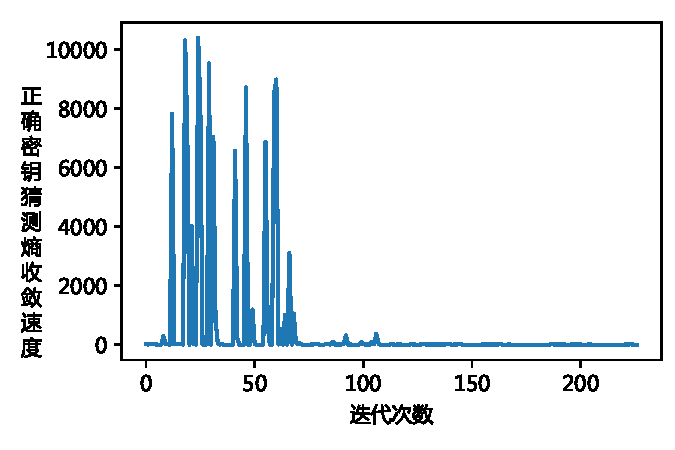
\includegraphics[width=\textwidth]{convratedpav4}
			\caption{DPA v4}
			\label{fig:convratedpav4}
		\end{subfigure}%
		~% add desired spacing
		\begin{subfigure}[b]{\trif\textwidth}
			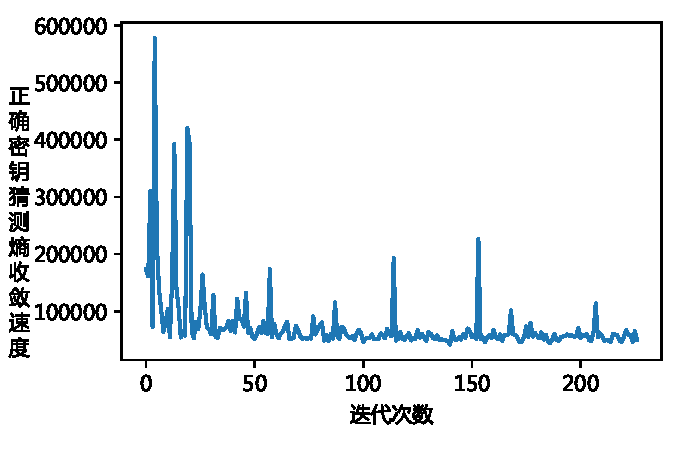
\includegraphics[width=\textwidth]{convrateaeshd}
			\caption{AES\_HD}
			\label{fig:convrateaeshd}
		\end{subfigure}
		~% add desired spacing
		\begin{subfigure}[b]{\trif\textwidth}
			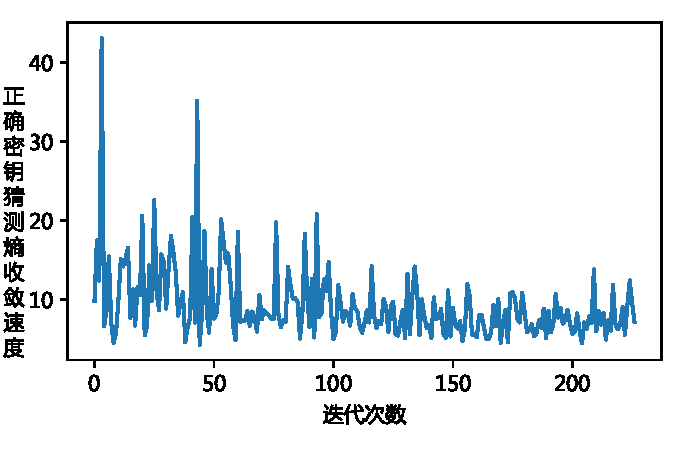
\includegraphics[width=\textwidth]{convrateaesrd}
			\caption{AES\_RD}
			\label{fig:convrateaesrd}
		\end{subfigure}
		\\% line break
		\begin{subfigure}[b]{\trif\textwidth}
			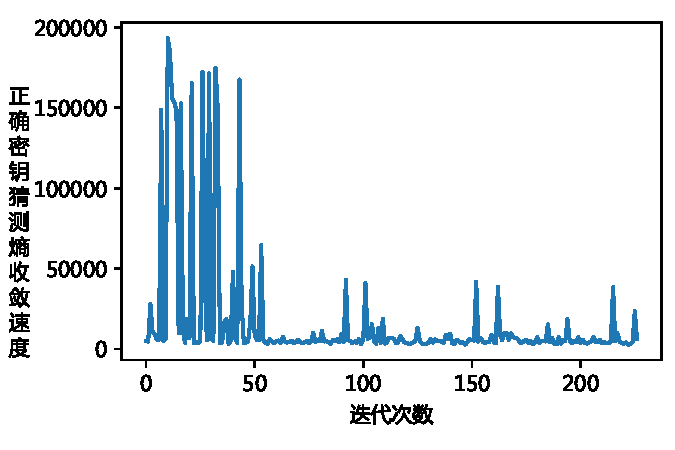
\includegraphics[width=\textwidth]{convrateascad0}
			\caption{ASCADf(N=0)}
			\label{fig:convrateascad0}
		\end{subfigure}%
		~% add desired spacing
		\begin{subfigure}[b]{\trif\textwidth}
			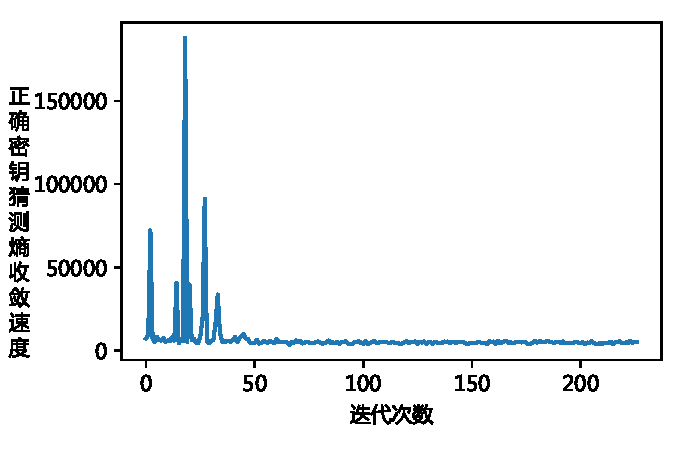
\includegraphics[width=\textwidth]{convrateascad50}
			\caption{ASCADf(N=50)}
			\label{fig:convrateascad50}
		\end{subfigure}
		~% add desired spacing
		\begin{subfigure}[b]{\trif\textwidth}
			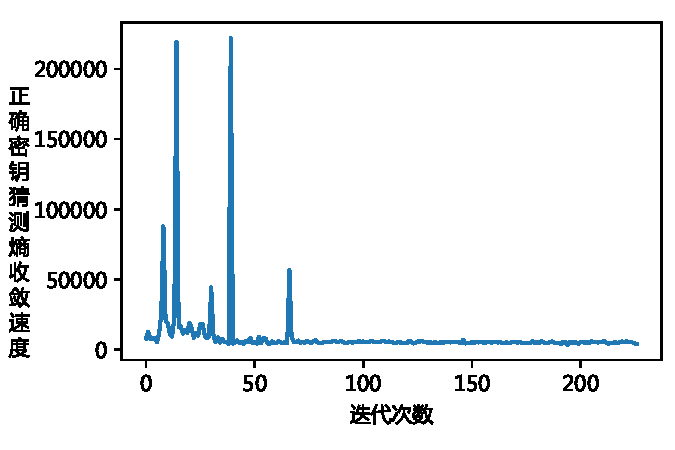
\includegraphics[width=\textwidth]{convrateascad100}
			\caption{ASCADf(N=100)}
			\label{fig:convrateascad100}
		\end{subfigure}
		\\% line break
		\bicaption{\enspace 深度学习训练过程的猜测上收敛速度曲线}{\enspace Curve of $convrate$ in Deep learning training process}
		\label{fig:convrateit}
	\end{figure}
	
	从\figureref{fig:convratedpav4},\figureref{fig:convrateaeshd},\figureref{fig:convrateascad0},\figureref{fig:convrateascad50}和\figureref{fig:convrateascad100}中可以看出,在搜索DPA v4、AES\_HD、ASCADf(N=0/N=50/N=100)数据集的最优数据增强策略参数时,在较早的阶段就达到较好的解并保持稳定,表明搜索快速收敛且找到了较优解。因此,在实际应用通用数据增强方法时可以减小迭代次数和提高退火速度以节省时间,并在攻击效果不受影响的前提下进行优化。\figureref{fig:convrateaesrd}展示了对AES\_RD数据集的搜索结果,攻击代价趋于稳定,在实际应用通用数据增强方法时可以不改变或略微增加迭代次数和降低退火速度来优化结果。
	
	可以看出,随着迭代次数的增加,代价逐渐降低并趋于稳定,这说明对于现有的数据集,将迭代次数设定为227可以使主控制器搜索出稳定的结果。
	
	本研究使用框架搜索到的所研究数据集的最佳数据增强策略参数如\tableref{tab:paras}所示。针对不同算法实现的能量迹,数据增强策略参数各异。参数的大致范围与理论一致,而其具体数值有必要使用本文通用数据增强方法进行搜索。
	
	\begin{table}[!h]
		\bicaption{\enspace 搜索到的最优数据增强策略参数}{\enspace Searched DA policy parameters}
		\label{tab:paras}
		\centering
		%\footnotesize% fontsize
		%\setlength{\tabcolsep}{4pt}% column separation
		%\renewcommand{\arraystretch}{1.2}%row space
		\small 
		\begin{tabular}{cc|cccccc}
			\hline
			\multicolumn{2}{c|}{\multirow{2}{*}{参数数值}} &\multirow{2}{*}{DPA v4}&\multirow{2}{*}{AES\_HD}&\multirow{2}{*}{AES\_RD}& \multicolumn{3}{c}{ASCAD} \\
			%\cline{3-5}
			\multicolumn{2}{c|}{}&&&&N=0 & N=50 & N=100 \\
			\hline
			\multirow{6}{*}{数据增强策略参数}
			&$p_{ro}$&0.676&0.720&0.762&0.161&0.749&0.621\\
			&$m_{ro}$&137&9&1&6&76&55\\
			&$p_{an}$&0.144&0.156&0.579&0.0761&0.444&0.774\\
			&$m_{an}$&   0&0.0523&0.345&0.522&0.0790&0.530\\
			&$p_{os}$&0.706&0.617&0.879&0.0579&0.0669&0.147\\
			&$m_{os}$&$10^{-5}$&0.399&0.0795&7.753&4.015&10\\
			\hline
			
		\end{tabular}   
	\end{table}

	\section{通用数据增强方法在AES算法实现分析中的实证研究}\label{sec:realexp}
	
	本文方法进行实证研究过程中,使用的机器配置如下:处理器型号为Intel(R) Xeon(R) CPU E5-2667 v4 @ 3.20GHz,内存大小252GB,操作系统版本为CentOS release 6.6 (Final)。本文方法使用Python(版本为3.6.2)作为编程语言进行实现,其中深度学习模型通过Keras\footnote{资料来源:keras \href{https://pypi.org/project/keras}{https://pypi.org/project/keras}。}开源框架进行实现。

	DL-SCA的攻击阶段与深度学习中的测试阶段有一定相似之处但并不完全相同。如\figureref{fig:dltestphase}和\figureref{fig:mydlscatest}所示,在深度学习训练出的模型对测试数据进行预测之后,还需要组合多条能量迹或电磁迹的信息进一步对算法密钥进行估计,从而计算侧信道领域的评价指标以评估侧信道分析技术效果,在本研究中,使用\chenggongtiaoshu 作为指标评估DL-SCA的效果,\chenggongtiaoshu 越小,那么DL-SCA效果越好。

	\begin{figure}[!h]
		\centering
		\begin{tikzpicture}[node distance=45pt, auto]
			% 定义节点样式
			\tikzstyle{reg} = [rectangle, draw,text centered]
			\tikzstyle{block} = [draw, rounded corners,align=center]
			\tikzstyle{data} = [draw, trapezium, trapezium left angle=70, trapezium right angle=110,align=center]
			\tikzstyle{arrow} = [thick,->,>=stealth]
			
			% 绘制节点
			\node [reg] (hyperparareg) {超参数寄存器};
			\node [block,below of =hyperparareg] (trained) {深度神经网络};
			\node [reg, left=70pt of trained] (parareg) {参数寄存器};
			\node [data, below of=trained] (dataset) {数据集};
			\node [block, right=100pt of dataset] (keypred) {密钥预测器};
			\node [block, below of =dataset] (keycalc) {密钥计算器};
			\node [block, below =50pt of keypred] (cmp) {侧信道分析\\指标计算器};
			
			%\node [block, below of=valacc, xshift=2cm] (testacc) {测试集准确率计算器};
			
			% 绘制箭头
			\draw [arrow] (dataset) -- node[right] {测试数据} (trained);
			\draw [arrow] (dataset) -- node[left] {测试标签(敏感中间值)} (keycalc);
			\draw [arrow] (dataset) -- node[pos=0.5,above] {算法输入、输出} (keypred);
			\draw [arrow] (dataset) -- ++(0:100pt) |- (keycalc);
			%\draw [arrow] (dataset) -- node[above] {测试数据} (pretrained);
			\draw [arrow] (trained) -| node[pos=0.3,above] {测试数据的标签预测结果} (keypred);
			\draw [arrow] (hyperparareg) -- node[right]{网络超参数}(trained);
			\draw [arrow] (parareg) -- node[above]{神经元参数}(trained);
			
			\draw [arrow] (keypred) -- node[right]{密钥预测值}(cmp);
			\draw [arrow] (keycalc) |- node[pos=0.7,below]{算法密钥}(cmp);
			\draw [arrow] (cmp) --node[pos=0.5, right] {\chenggongtiaoshu } ++(270:40pt);
		\end{tikzpicture}
		\bicaption{\enspace 攻击AES的深度学习测试阶段}{\enspace DL test phase for SCA on AES}
		\label{fig:mydlscatest}
	\end{figure}


	\subsection{通用数据增强方法的技术效果}
	
	本研究尝试了1倍、5倍、10倍、20倍四种增广倍数$C$(见\algorithmref{alg:combined-da}输入,$T^{agmt}=T*C$,$T$是数据增强前训练样本数量)以探索最优的实验条件。
	
	不同实验条件下DL-SCA的性能如\tableref{tab:adamtd}所示,表格中加粗的结果表示在对应数据集上取得的最优技术效果。根据实验结果可以看出,增广倍数为10倍或20倍时能取得最小的\chenggongtiaoshu 。例如,在分析引入随机延迟的软件AES实现数据集AES\_RD时,选取C=20。这样一来,在仅提供20000条能量迹用于DL-SCA的建模时,采用本文提出的数据增强方法可以将\chenggongtiaoshu 减小到5。在每个数据集上取得的最优技术效果的猜测熵曲线如\appfigureref{appfig:adadlsca}所示。
	
	\begin{table}[!h]
		\bicaption{\enspace 采用通用数据增强方法的DL-SCA的性能}{\enspace Performance of DL-SCA with general DA method}
		\label{tab:adamtd}
		\centering
		\footnotesize% fontsize
		%\setlength{\tabcolsep}{4pt}% column separation
		%\renewcommand{\arraystretch}{1.2}%row space
		\begin{tabular}{cc|cccccc}
			\hline
			\multirow{2}{*}{性能指标}&\multirow{2}{*}{增广倍数} &\multirow{2}{*}{DPA v4}&\multirow{2}{*}{AES\_HD}&\multirow{2}{*}{AES\_RD}& \multicolumn{3}{c}{ASCAD} \\
			%\cline{3-5}
			\multicolumn{2}{c|}{}&&&&N=0 & N=50 & N=100 \\
			\hline
			\multirow{2}{*}{\shortstack{数据增强前\\训练样本数量}}&&\multirow{2}{*}{4000}&\multirow{2}{*}{45000}&\multirow{2}{*}{20000}&\multirow{2}{*}{45000}&\multirow{2}{*}{45000}&\multirow{2}{*}{45000}\\
			&&&&&&&\\
			\hline
			\multirow{4}{*}{\chenggongtiaoshu }
			&1&9&1358&11&>300&>400&>400\\
			&5&4&959&6&>300&273&>400\\
			&10&\textbf{3}&\textbf{880}&6&\textbf{197}&305&\textbf{288}\\
			&20&\textbf{3}&898&\textbf{5}&206&\textbf{193}&382\\
			\hline
			
		\end{tabular}   
	\end{table}
	
%	使用本文提出的通用数据增强方法搜索最优的数据增强策略参数,使用这些参数对训练集进行组合式数据增强,使用数据增强后的训练集训练深度学习模型后,训练后的深度学习模型进行攻击的结果如\appfigureref{appfig:adadlsca}所示。我们从\appfigureref{appfig:adadlsca}提取\chenggongtiaoshu 的信息,将它们列举在\tableref{tab:adamtd}中。
%	
%	\begin{table}[!h]
%		\bicaption{\enspace 使用通用数据增强方法时DL-SCA的性能}{\enspace Performance of DL-SCA with adaptive DA method}
%		\label{tab:adamtd}
%		\centering
%		%\footnotesize% fontsize
%		%\setlength{\tabcolsep}{4pt}% column separation
%		%\renewcommand{\arraystretch}{1.2}%row space 
%		\begin{tabular}{c|cc}
%			\hline
%			数据集名称&数据增强前的训练样本数量&\chenggongtiaoshu \\
%			\hline
%			DPA v4    &4000&3\\
%			\hline
%			AES\_HD   &45000&860\\
%			\hline
%			\multirow{2}{*}{AES\_RD}
%				&5000&10\\
%				&20000&5\\
%			\hline
%			\multirow{2}{*}{ASCADf(N=0)}
%				&38400&255\\
%				&45000&197\\
%			\hline
%			ASCADf(N=50)&45000&156\\
%			\hline
%			ASCADf(N=100)&45000&288\\
%			\hline
%		\end{tabular}
%	\end{table}
	\subsection{无数据增强的技术效果}
	不进行数据增强,直接训练深度学习模型,并使用训练后的深度学习模型进行攻击的结果如\appfigureref{appfig:origindlsca}所示。我们从\appfigureref{appfig:origindlsca}提取\chenggongtiaoshu 的信息,将它们列举在\tableref{tab:originmtd}中。
	
	\begin{table}[!h]
		\bicaption{\enspace 无数据增强时DL-SCA的性能}{\enspace Performance of DL-SCA without any DA method}
		\label{tab:originmtd}
		\centering
		%\footnotesize% fontsize
		%\setlength{\tabcolsep}{4pt}% column separation
		%\renewcommand{\arraystretch}{1.2}%row space 
		\begin{tabular}{c|cc}
			\hline
			数据集名称&训练样本数量&\chenggongtiaoshu \\
			\hline
			DPA v4    &4000&4\\
			\hline
			AES\_HD   &45000&1118\\
			\hline
			\multirow{2}{*}{AES\_RD}
			&5000&12\\
			&20000&5\\
			\hline
			\multirow{2}{*}{ASCADf(N=0)}
			&38400&294\\
			&45000&259\\
			\hline
			ASCADf(N=50)&45000&369\\
			\hline
			ASCADf(N=100)&45000&304\\
			\hline
		\end{tabular}
	\end{table}

	对比\tableref{tab:adamtd}和\tableref{tab:originmtd}相对应(建模能量迹条数相同)的表项,可以观察到本文提出的方法在AES\_HD、DPA v4、ASCADf三种数据集共五个场景上使得\chenggongtiaoshu 减少21\%、25\%、24\%、48\%以及5\%。这说明与未采用数据增强的方法相比,采用本文提出的通用数据增强方法在无防护、高噪声、随机延迟或掩码防护的密码算法实现的DL-SCA场景中,能够显著提升侧信道分析技术效果,减少\chenggongtiaoshu 。上述结果表明,本文提出的数据增强方法的通用性。
	
	而在AES\_RD数据集上,\chenggongtiaoshu 保持不变,可能的原因是迭代次数不足。从\figureref{fig:convrateaesrd}中可以看出,AES\_RD数据集上攻击代价的在227的迭代次数下还未稳定;\figureref{fig:convratedpav4},\figureref{fig:convrateaeshd},\figureref{fig:convrateascad0},\figureref{fig:convrateascad50}和\figureref{fig:convrateascad100}中,其他数据集上攻击代价在227的迭代次数下已经达到稳定。出于公平比较的目的,我们限制了主控制器迭代次数为227。
	
%如果使用通用数据增强方法的DL-SCA的数据增强前的训练样本数量和无数据增强时DL-SCA的训练样本数量相同,那么前者的\chenggongtiaoshu 不高于后者的\chenggongtiaoshu 。例如,对于DPA v4数据集所对应的无防护软件实现,\tableref{tab:adamtd}的结果表明如果攻击者可以采集4000条迹进行建模,那么使用通用数据增强方法时,DL-SCA可以使用3条迹就完成攻击。同样对于DPA v4数据集所对应的无防护软件实现,\tableref{tab:originmtd}的结果表明如果攻击者可以采集4000条迹进行建模,那么不使用数据增强方法时,DL-SCA需要4条迹才能完成攻击。
%
%	通用数据增强相比于无数据增强,可以在攻击者采集相同数量的样本的情况下,使得深度学习模型对信息泄漏的刻画更准确,从而减少\chenggongtiaoshu 。本文提出的方法在AES\_HD、DPA v4、ASCADf(N=0)、ASCADf(N=50)、ASCADf(N=100)五个数据集上使得\chenggongtiaoshu 相比于无数据增强减少23\%、25\%、24\%、58\%以及5\%,在AES\_RD数据集上使得\chenggongtiaoshu 与无数据增强相当。
	\subsection{其他数据增强方法的技术效果}

	本文还将采用本文提出通用数据增强方法的DL-SCA和近年来采用其他数据增强方法的DL-SCA结果进行比较,以说明本文通用数据增强方法的优势。
	
	使用其他文献中的方法进行数据增强,最终进行DL-SCA的结果如\tableref{tab:othermtd}所示。
	
	%使用其他文献中的方法进行数据增强,最终进行DL-SCA的结果如\tableref{tab:othermtd}所示。在\tableref{tab:othermtd}中,“文献\normalcite{Cagli17}”表示本研究复现的\citet{Cagli17}位移变形和添加删除变形的数据增强方法,这是因为原文并无DPA v4、AES\_HD、AES\_RD和ASCADf数据集上的实验结果。“文献\normalcite{Kim19}”表示本研究复现的\citet{Kim19}添加高斯白噪声的数据增强方法,这是因为复现时使用的网络模型优于论文原本使用的网络模型,复现论文方法的实验结果优于论文所汇报的实验结果。“文献\normalcite{Won20}”表示\citet{Won20}使用合成少数类过采样法及其变体的数据增强方法,表项直接使用论文所汇报的实验结果。“文献\normalcite{Luo21}”表示\citet{Luo21}使用混淆技术的数据增强方法,表项直接使用论文所汇报的实验结果。“文献\normalcite{Mukhtar22}”表示\citet{Mukhtar22}基于条件生成对抗网络和连体网络的数据增强方法,表项直接使用论文所汇报的实验结果。

	\begin{table}[!h]
		\bicaption{\enspace 使用其他数据增强方法时DL-SCA的性能}{\enspace Performance of DL-SCA with other DA method}
		\label{tab:othermtd}
		\centering
		%\footnotesize% fontsize
		%\setlength{\tabcolsep}{4pt}% column separation
		%\renewcommand{\arraystretch}{1.2}%row space
		\scriptsize
		\begin{tabular}{cc|cccccc}
			\hline
			\multirow{2}{*}{数据增强方法} &\multirow{2}{*}{性能指标} &\multirow{2}{*}{DPA v4}&\multirow{2}{*}{AES\_HD}&\multirow{2}{*}{AES\_RD}& \multicolumn{3}{c}{ASCAD} \\
			%\cline{3-5}
			\multicolumn{2}{c|}{}&&&&N=0 & N=50 & N=100 \\
			\hline
			\multirow{2}{*}{Cagli等\citep{Cagli17}}
				&数据增强前训练样本数量       &4000&45000&20000&45000&45000&45000\\
				&\chenggongtiaoshu      &5&1252&7&219&328&364        \\
			\hline
			\multirow{2}{*}{Kim等\citep{Kim19}}
				&数据增强前训练集大小       &4000&45000&20000&45000&45000&45000\\
				&\chenggongtiaoshu     &5&1127&5&249&276&346\\
			\hline
			\multirow{2}{*}{Won等\citep{Won20}}
				&数据增强前训练集大小       &/&/&5000&/&/&45000\\
				&\chenggongtiaoshu     &/&/&15&/&/&190\\
			\hline
			\multirow{2}{*}{Luo等\citep{Luo21}}
				&数据增强前训练集大小       &/&/&50000&50000&50000&50000\\
				&\chenggongtiaoshu     &/&/&>1000&1250&4000&7000\\
			\hline
			\multirow{2}{*}{Mukhtar等\citep{Mukhtar22}}
				&数据增强前训练集大小       &/&/&/&38400&/&/\\
				&\chenggongtiaoshu     &/&/&/&410&/&/\\
			\hline
			
		\end{tabular}   
	\end{table}

	对比\tableref{tab:adamtd}、\tableref{tab:originmtd}和\tableref{tab:othermtd}相对应(建模能量迹条数相同)的表项,可以观察到在AES\_RD、AES\_HD、DPA v4、ASCADf(N=0/N=50)四种数据集五个场景中,采用本文方法的DL-SCA\chenggongtiaoshu 减小比例最高。与已有最好的数据增强方法相比,采用本文提出的数据增强方法可将实施侧信道分析的\chenggongtiaoshu 分别降低0\%、22\%、40\%、10\%、30\%。这说明,与采用了数据增强的已知最好方法相比,采用本文提出的通用数据增强方法,在无防护、高噪声或掩码防护型密码算法实现的DL-SCA场景中,本文提出的数据增强方法更高效。

	在ASCADf(N=100)数据集上,与最好的数据增强方法Won等\citep{Won20}相比,采用本文提出的数据增强方法使得实施侧信道分析的\chenggongtiaoshu 增加52\%。可能的原因是Won等\citep{Won20}尝试85种SMOTE算法的不同变体找到一种较优的数据增强方法,而本文方法仅对三种数据增强子策略进行组合式数据增强并搜索最优参数。因此在实际应用中,本文方法更容易满足时间效率的需求,可以高效地找到合适的数据增强策略参数。除此之外,增加数据增强子策略到通用数据增强方法的数据增强单元,有可能使得本文方法达到与Won等\citep{Won20}匹配的结果。
	%通用数据增强相比于无数据增强,可以在攻击者采集相同数量的样本的情况下,有较大的可能使得深度学习模型对信息泄漏的刻画更准确,从而减少\chenggongtiaoshu 。本文提出的方法在AES\_HD、DPA v4、ASCADf(N=0)、ASCADf(N=50)四个数据集上使得\chenggongtiaoshu 相比于已知最好的数据增强方法分别减少24\%、40\%、10\%、43\%,在AES\_RD数据集上使得\chenggongtiaoshu 与已知最好的数据增强方法相当,在ASCADf(N=100)数据集上使得\chenggongtiaoshu 相比于已知最好的数据增强方法增加了52\%。
	\section{本章小结}
	针对已有数据增强方法的参数选取高度依赖专家知识,且只适用于特定算法实现数据集的实际问题,本文提出一种通用数据增强方法,该方法能够自适应地搜索数据增强策略参数,增广出新的样本用于训练深度学习模型,进而提升DL-SCA效果。本文通过对应于多种攻击难度的AES算法实现的数据集对新提出的通用数据增强方法进行了验证。实验结果表明,与无数据增强或目前已知的数据增强方法相比,通用数据增强方法可以使得\chenggongtiaoshu 最多降低48\%。
}
\chapter{面向双界面商用智能卡ECDSA实现的电磁分析方法}\label{chap:search2}{
	密码硬件单元物理安全性检测评估结果的准确性和可靠性,高度依赖于所使用的先进、高效的侧信道分析方法。%因此,为确保密码硬件单元物理安全性评估体系的准确性、可靠性和前沿性,有必要持续深入研究并发展先进、高效的侧信道分析方法。%DL-SCA是一类强大的侧信道分析方法,但实际应用DL-SCA时还存在DL-SCA量化指标选择不合理、计算量巨大、采集电磁迹消耗的时间长、恢复私钥的理论时间长等问题。
	
	%本文以分析一款双界面商用智能卡为例,开展了面向基于深度学习侧信道分析的数据增强方法应用示例研究,提出了新的预处理技术并应用了\chapref{chap:search1}的方法和基于假设检验的敏感信息泄漏估计方案,有效提升了DL-SCA在双界面商用智能卡分析场景中的技术效果。在缺少双界面商用智能卡产品设计细节、ECDSA实现所使用的防护对策未知的情况下,成功实现了一款具有ECDSA签名功能的双界面商用智能卡的破解。本文首先进行信息泄漏预处理,将DL-SCA的训练阶段计算量减小到$1.727\cdot10^{11}$浮点运算次数,为原来的0.16\%,DL-SCA变得可行。在不改进网络架构的情况下,使用数据增强进行DL-SCA可以将恢复双界面商用智能卡ECDSA签名信息泄漏的\zyx 由91.35\%提升到95.50\%。使用基于假设检验的估计方案后,\zyx 进一步提升到100\%。这使得从理论上讲,在侧信道分析之后使用格方法恢复双界面商用智能卡ECDSA私钥的时间会从超过七百万年减少到12.5年,再进一步减少到400秒,包含采样时间在内的攻击总时间变为4天,深度学习侧信道方法在双界面商用智能卡分析场景中的攻击成本显著降低。
	
	%具体来说,本文选择DL-SCA作为主体,选取ECDSA中的一次性随机数泄漏作为攻击目标,使用格基规约从一次性随机数泄漏推算私钥。在这个过程中,提出模数转换、去抖动、高斯模糊多种预处理技术及其组合实现特征点(Point of Interest, POI)高效、准确地提取,使用面向基于深度学习侧信道分析的数据增强方法减少对训练数据的依赖,依据ECDSA签名实现本身的特点定制最有助于恢复私钥的估计方法提高格基规约的成功率。最终成功在可接受的时间内恢复了双界面商用智能卡ECDSA私钥。本文的分析思路和技术方法可以应用于其他类型的双界面商用智能卡分析场景中,为开展其他类似密码硬件单元的分析与破解提供可行的思路和真实的案例。
	
		
	本文以分析一款双界面商用智能卡为例,从\jiaodu 开展了电磁分析方法研究,解决了实际场景侧信道分析时存在样本数量不足和单个样本过大的问题,减少了DL-SCA时间,提高了DL-SCA\zyx。该方法包括预处理、模板构建以及模板匹配三个阶段。
	%在分析双界面商用智能卡的ECDSA实现时,需要将侧信道分析与格方法结合才可能利用当前实验环境在可接受的时间范围内恢复私钥。在实际分析时,电磁迹采样点多导致深度学习模型训练时间长达315天,电磁迹特征点不明显导致运用格方法恢复ECDSA私钥的时间达到约$2\times10^{85}$年,仍然超过可接受的时间范围。本文提出并使用\yuchuli 预处理技术,以增加3天的预处理时间为代价,将DL-SCA时间由315天减小为8分钟,将运用格方法的时间由约$2\times10^{85}$年减小到约$7\times10^{6}$年。本文使用\chapref{chap:search1}的面向基于深度学习侧信道分析的通用数据增强方法,以增加2分钟的数据增强时间和1小时的DL-SCA时间为代价,将运用格方法的时间由约$7\times10^{6}$年减小到约12.5年。本文提出并使用\jiashejianyanguji 方案,将运用格方法的时间由约12.5年减小到400秒。本文仅用4天就恢复了ECDSA私钥,其分析思路和技术方法可以应用于其他类型的双界面商用智能卡分析场景中,为开展其他类似密码硬件单元的分析与破解提供可行的思路和真实的案例。
	
	预处理阶段采用了\poifanwei 和\yuchuli 两项技术,首先运用了\poifanwei 技术将特征点范围从5000万缩小到1.8万,接着使用\yuchuli 技术提取了特征点,完成了电磁迹的预处理,成功构造了用于深度学习的数据集。
	模板构建阶段采用了\shujuzengqiang,选择最优的数据增强策略参数对现有数据集中的训练集进行数据增强,使得实际攻击时在不额外采集电磁迹的情况下将DL-SCA的\zyx 由91.35\%提高到95.50\%。
	模版匹配阶段采用了\jiashejianyanguji ,利用格方法攻击目标双界面商用智能卡ECDSA实现的特点(对错误预测为比特0敏感,错误预测为比特1不敏感),使用更严格的标准估计比特0。在五次实验中,在训练完成后样本数量为5000的测试集中平均有981个敏感中间值估计值为0,其准确率为100\%;有4019个敏感中间值估计值为1,其准确率为75.89\%。\zyx 达到了100\%。
	
	
	在现有实验环境下,成功实现了对型号为J3D081的Java卡的电磁分析,在1天内采集5000条电磁迹、3天内进行电磁迹预处理得到样本数量为十万的数据集、137秒内对数据集中的训练集进行数据增强、1小时内实施DL-SCA恢复nonce比特。实际攻击时,利用被恢复的比特泄漏可以过滤出119个含有连续4比特0的nonce,达到了使用由nonce部分比特恢复私钥的格方法的条件。本文分析思路和技术方法可以应用于其他类型的双界面商用智能卡分析场景中,为开展其他类似密码硬件单元的分析与破解提供可行的思路和真实的案例。
	
	\secref{sec:vulnerable}介绍了作为本文攻击目标的双界面商用智能卡ECDSA实现的预备知识,\secref{sec:hardpoint}介绍了攻击智能卡存在的难点,\secref{sec:solution}详细说明了解决现有问题的技术方案,\secref{sec:ecdsaresult}以双界面商用智能卡ECDSA实现为例,汇报了实施面向智能卡电磁分析的技术效果。
	
%	\begin{table}[!h]
%		\bicaption{\enspace 攻击智能卡待解决的问题}{\enspace Nuts to crack in attacking the smart card}
%		\label{tab:problemset}
%		\centering
%		\scriptsize% fontsize
%		%\setlength{\tabcolsep}{4pt}% column separation
%		%\renewcommand{\arraystretch}{1.2}%row space 
%		\begin{tabular}{ll|ll}
%			\hline
%			\multicolumn{2}{c|}{现有问题} & 不解决会造成的后果&本文的解决方案\\
%			\hline
%			实验条件&示波器采样深度低&攻击所需的电磁迹增加&暂无解决方案\\
%			\hline
%			\multirow{2}{*}{量化指标选择}&准确率等指标不适合本文&\multirow{2}{*}{分析技术的优化方向错误}&\multirow{2}{*}{使用敏感信息泄漏估计\zyx }\\
%			&猜测熵等指标难以定义&&\\
%			\hline
%			\multirow{3}{*}{分析技术选择}&缺少计算资源&无法进行DL-SCA&提取特征点,减小计算量\\
%			&依赖大量样本进行训练&增加采集电磁迹的时间开销&使用\chapref{chap:search1}的数据增强方法\\
%			&极大似然估计不适合本文&增加运用格方法恢复私钥的时间&设定基于假设检验的估计方案\\
%			\hline
%		\end{tabular}
%	\end{table}

	\section{ECDSA攻击预备知识}\label{sec:vulnerable}
	\subsection{智能卡ECDSA签名实现推测}
	
	作为研究目标的智能卡所属的产品家族(Product Family)为J3D081,它是符合ISO7816\citep{ISO/IEC7816}与ISO14443 A\citep{ISO/IEC14443}规范的双界面的Java产品,其JCOP版本是Java Card3.0.1,GlobalPlatform版本是2.2.1。该智能卡使用了SmartMX\citep{p5x}安全微控制器芯片。Roche等\citep{Roche21}对同样使用SmartMX的两款智能卡进行过研究,并对其在ECDSA算法中的数乘实现进行了分析和猜想。因为芯片型号完全相同,我们认为J3D081智能卡与Roche等\citep{Roche21}研究的智能卡中ECDSA中的数乘实现也相同。
	
	Roche等\citep{Roche21}对智能卡中数乘实现进行了分析,依据分析结果对签名操作的数乘算法进行了推测。签名操作的数乘$\nonce\cdot G$应当执行如下步骤进行了计算:
	
	\begin{itemize}
		\item 使用\algorithmref{alg:encodek}将一次性随机数$\nonce$转化为长度为129的编码形式$\left\{\tilde{\nonce}_0,\tilde{\nonce}_1,\dots,\tilde{\nonce}_{128}\right\}$。
		\item 使用\algorithmref{alg:improvesignscalar}计算数乘结果。
	\end{itemize}
	
	\begin{breakablealgorithm}
		\caption{窗口大小为2的大数编码算法}\label{alg:encodek}
		\begin{algorithmic}[1]
			\Statex \textbf{输入:} $\multiplier$:被编码的整数
			\Statex \textbf{输入:} $cl$:目标编码的长度
			\Statex \textbf{输出:} $\left\{\tilde{\multiplier}_0,\tilde{\multiplier}_1,\dots,\tilde{\multiplier}_i,\dots, \tilde{\multiplier}_{cl-1}\right\}$:$\multiplier$的长度为$cl$的编码形式
			\State 计算$\multiplier$的二进制表示$\sum\limits_{i=0}^{2cl-1}\multiplier_i2^{2cl-i-1}=\multiplier$
			\For{$i := 0, \dots, cl-1$}
			\State $\tilde \multiplier_i:=2\multiplier_i+\multiplier_{i+cl}$
			\EndFor
			\State \Return $\left\{\tilde{\multiplier}_0,\dots,\tilde{\multiplier}_i,\dots, \tilde{\multiplier}_{cl-1}\right\}$
		\end{algorithmic}
	\end{breakablealgorithm}

	\algorithmref{alg:encodek}实际上在ECDSA签名和验签过程中都被使用,它的作用是对一个大整数进行表达形式上的调整,使得这个调整后的输出结果可以直接作为其他算法的输入。在签名操作中,\algorithmref{alg:encodek}的输入$\multiplier=\nonce,cl=129$。

	\begin{algorithm}[!h]
		\caption{改进后签名操作的数乘算法}\label{alg:improvesignscalar}
		\begin{algorithmic}[1]
			\Statex \textbf{输入:} $\left\{\tilde{\nonce}_0,\tilde{\nonce}_1,\dots,\tilde{\nonce}_j,\dots, \tilde{\nonce}_{128}\right\}$:一次性随机数$\nonce$的长度为129的编码形式
			\Statex \textbf{输入:} $G_1,G_2,G_3,G_4$:预计算的椭圆曲线$E$上的点
			\Statex \textbf{输出:} $\nonce\cdot G$:基点$G$与一次性随机数$\nonce$数乘的结果
			\State $S:=G_1$
			\For{$j:=1,\dots , 128$}
			\State $S:=2\cdot S$
			\If {$\tilde \nonce_j>0$}
			\State $\leakedmultiplier_j:=\tilde \nonce_j$
			\State $S:=S+G_{\leakedmultiplier_j}$\Comment{$\leakedmultiplier_j$存在泄漏}
			\Else
			\State $\leakedmultiplier_j\stackrel{\$}\gets\{1,1,2,3\}$\Comment{引入随机数}
			\State $Dummy:=S+G_{\leakedmultiplier_j}$\Comment{$\leakedmultiplier_j$存在泄漏}
			\EndIf
			\EndFor
			\If {$\tilde \nonce_0=0$}
			\State $S:=S-G_4$
			\Else
			\State $Dummy:=S-G_4$
			\EndIf
			\State \Return $S$
		\end{algorithmic}
	\end{algorithm}

	在签名操作中,\algorithmref{alg:improvesignscalar}的输入$\left\{\tilde{\nonce}_0,\tilde{\nonce}_1,\dots,\tilde{\nonce}_{128}\right\}$是\algorithmref{alg:encodek}的输出,$G_1,G_2,G_3,G_4$是不必重复计算的\footnote{这些值在确定椭圆曲线$E$和生成元$G$之后就可以预计算,将计算结果硬编码进外存。每次签名时,将外存的数据载入内存参与运算即可完成签名。因此这些值是不必重复计算的。}椭圆曲线$E$上的点,$G_1=G,G_2=2^{129}\cdot G,G_3=\left(2^{129}+1 \right) \cdot G,G_4=2^{128}\cdot G$,$G$是选定椭圆曲线$E$的同时所选定的生成元。
	\subsection{随机数部分泄漏的情况下基于格的ECDSA攻击背景}\label{subs:infoforlattice}
	
	有大量工作\citep{Howgrave-Graham01,Nguyen02,Nguyen03,Hlavac06,Brumley11,Mulder14,Benger14,Goudarzi16,Fan16,Ryan19,Jancar20,Moghimi20,Weiser20,Micheli20}研究了在随机数泄漏少量比特的情况下攻击ECDSA方案,它们的主要思想是利用签名中的随机数的泄漏构造扩展隐藏数问题\citep{Boneh96}的方程并使用格基规约求解。
	
	在本文中,为了恢复私钥,需要使用格方法从一次性随机数$\nonce$的泄漏求解私钥$\sk$。但是格方法本身不在本文研究范围内,因此只做大致描述。
	
	\begin{figure}[!h]
		\centering
		\small
		\begin{tikzpicture}[node distance=20pt]
			\node[draw, rounded corners,align=center]  (start)  {运算开始};
			\node[draw, trapezium, trapezium left angle=70, trapezium right angle=110,below=of start,align=center](inputleak){输入:用于构造方程的签名及其泄漏};
			\node[draw, below=of inputleak,align=center] (constructequ)  {构造方程};
			\node[draw, below=of constructequ,align=center] (solve)  {使用格基规约算法求解(近似)最短向量};
			\node[draw, below=of solve,align=center] (calcd)  {根据(近似)最短向量求解私钥$\hat \sk$};
			\node[draw, diamond, aspect=2, below=of calcd,align=center]     (chkd)  {$\hat \sk\cdot G=\pk$?};
				
			\node[draw, trapezium, trapezium left angle=70, trapezium right angle=110,align=center]at ([xshift=-40pt,yshift=-35pt]chkd.south west)(success){输出:"求解成功",$\sk=\hat \sk$};
			\node[draw, trapezium, trapezium left angle=70, trapezium right angle=110,align=center]at ([xshift=40pt,yshift=-35pt]chkd.south east)(fail){输出:"求解失败"};
			\node[draw, rounded corners, below=50pt of chkd,align=center]  (end) {运算结束};
				
			\draw[->] (chkd) -|node[midway,very near start,above] {是} (success);
			\draw[->] (chkd) -|node[midway,very near start,above] {否} (fail);
				
			\draw[->] (success) |- (end);
			\draw[->] (fail) |- (end);
			\graph{
				(start)->(inputleak)->(constructequ)->(solve)->(calcd) -> (chkd);
			};
		\end{tikzpicture}
		\bicaption{\enspace 利用随机数部分泄漏进行基于格的ECDSA攻击流程图}{\enspace Flowchart of lattice-based ECDSA attacks with partial knowledge of the nonces}
		\label{fig:solver}	
	\end{figure}
	
	运用一次格方法从一次性随机数$\nonce$的泄漏求解私钥$\sk$的过程如\figureref{fig:solver}所示。它首先依据输入构造方程,其次调用格基规约算法求解近似最短向量,然后将近似最短向量视为最短向量以计算出私钥,接着通过公钥对私钥进行验证,最后输出验证结果。之所以需要验证是因为有多种原因会导致求解出错误的私钥。运用一次格方法是伯努利实验,它有一定的失败概率。但是在实际中,运用格方法次数的唯一限制因素是攻击者提供的用于攻击的时间。在攻击时间内,攻击者可以尝试多次运用格方法,直到恢复私钥为止。在这种情况下,只论成功率的大小已经意义不大,因为从理论上讲只要提供足够长的攻击时间,就一定能恢复私钥。%假如运用一次格方法的成功概率固定,且每次运用格方法是否成功互相独立,那么攻击者运用格方法的次数应当服从二项分布。
	
	运用一次格方法的主要时间开销来自于执行其中的格基规约算法。当前的格基规约算法是多项式时间复杂度的近似算法,它有三方面的使用限制:
	
	\begin{enumerate}
		\item 格上的方程应当合理且信息量充足,否则求解失败;
		\item 格上的方程不能含有错误,否则求解失败;
		\item 即使格上的方程合理、信息量充足且不含错误,也可能求解失败。
	\end{enumerate}
	
	如果格上的方程信息量不充足,那么方程欠定,会有无穷多种可行解,因此无法找到所需要的正解,求解失败。如果方程含有错误,会导致运算过程出错,求解失败。在格上的方程信息量充足且不含错误的情况下,因为当前的格基规约算法是近似算法,本身就可能导致计算出的近似解不是正解,求解失败。方程不合理会导致算法执行过程中更可能做出错误的近似,计算出的近似解有更大的可能不是正解,求解失败。
	
	%不失一般性地,不妨假设在侧信道攻击之后仍然存在某些信息泄漏没有恢复\footnote{通常来说,侧信道攻击要求恢复每一处信息泄漏,因为即使存在偶然误差也可以通过平均的方法加以控制。但是对于ECDSA来说,一次性随机数互相独立、一次性随机数每个比特也互相独立,无法使用平均的方法控制随机误差。本文使用的格方法在仅恢复特定的一部分信息泄漏的情况下依然可以恢复私钥,因此本文不恢复每一处信息泄漏}。
	本文在侧信道分析之后会尝试多次运用格方法\footnote{格方法通常是指通过解决格问题来攻击密码系统,而在实践中,可能需要多次尝试和调整参数才能成功恢复私钥},直到成功恢复私钥:
	
	\begin{enumerate}
		\item 枚举每条签名,如果从对应的电磁迹中恢复的敏感中间值估计值$\hat{\tilde \nonce}_j,j=0,1,\dots,128$为0的次序中有连续4位的情况,那么记录这连续4位(如果有多个连续4位的情况,记录一个即可)的位置以及值\footnote{如果$\exists 0\le k<30-4,\hat{\nonce}^{(i)}_k=\hat{\nonce}^{(i)}_{k+1}=\hat{\nonce}^{(i)}_{k+2}=\hat{\nonce}^{(i)}_{k+3},i=0,1,\dots,T_a-1$,那么记录数据对$(i,k)$并同时记录第$i$条签名。},否则排除该签名(不用于后续攻击);
		\item \textbf{随机}选择75条保留下来的签名(如果保留下来的签名不足75条,那么无法求解,需要采集更多电磁迹加以解决);
		\item 利用这些签名的签名消息$hsh=H(m_0)$、签名$(r,s)$、连续4位的被恢复的一次性随机数比特泄漏所在位置以及值、椭圆曲线的阶$q$,构造格上的方程;
		\item 调用格基规约算法BKZ\citep{Schnorr91}进行格基规约,利用近似解求解私钥;
		\item 使用公钥验证私钥,如果验证成功返回私钥,如果验证失败返回第2步。
	\end{enumerate}

	\subsection{符号表示}\label{subs:ecdsasymbol}
	%本文不区分“估计”和“预测”两个概念。前者用于从假设检验的角度进行理论分析,后者用于描述实践中依据深度学习网络输出的概率向量推断敏感信息泄漏最可能的值的过程。
	%本文严格区分“预测”和“估计”两个概念。前者用于描述深度学习网络输出概率向量的过程,后者用于描述使用数理统计的方法,依据统计量(例如深度学习网络输出概率向量),判定是否接受与一个值(例如敏感中间值)有关的假设。
	
	本文严格区分“敏感中间值”和“敏感中间值估计值”两个概念。%b阳性率b、b阳性率b值、b阳性率b估计、b阳性率b估计值。%它们的关系如\figureref{fig:leakageill}所示。
	
%{	
%	\begin{figure}[!h]
%		\begin{center}
%			\begin{tikzpicture}[node distance=40pt, auto]
%				\tikzstyle{obj} = [draw, rounded corners,align=center]
%				\tikzstyle{var} = [rectangle, draw,text centered]
%				
%				\node[var] (leakage) {b阳性率b};
%				\node[obj,right=85pt of leakage] (leakageobj) {b阳性率b值};
%				\node[var,below= of leakage] (trace) {信息泄漏};
%				\node[obj,below= of leakageobj] (traceobj) {迹};
%				\node[obj,below= of traceobj] (leakageprobobj) {b阳性率b概率向量};
%				\node[obj,below= of leakageprobobj] (leakageestimateobj) {b阳性率b估计值};
%				\node[var]at (trace |- leakageestimateobj) (leakageestimate) {b阳性率b估计};
%				%		\node[var,below= of leakageestimate] (okleakageestimate) {可利用的b阳性率b估计};
%				%		\node[obj,below= of leakageestimateobj] (okleakageestimateobj) {可利用的b阳性率b估计值};
%				%		\node[var,below= of okleakageestimate] (usedleakageestimate) {被利用的b阳性率b估计};
%				%		\node[obj,below= of okleakageestimateobj] (usedleakageestimateobj) {被利用的b阳性率b估计值};
%				
%				\draw[dashed] (-60pt,50pt) rectangle (60pt,-200pt);
%				\node at (0,40pt) {随机变量};
%				
%				\draw[dashed] (102pt,50pt) rectangle (390pt,-200pt);
%				\node at (246pt,40pt) {样本值(评估者可以得到的信息)};
%				
%				\draw[dash dot] (105pt,-40pt) rectangle (387pt,-195pt);
%				\node at (320pt,-188pt) {攻击者可以得到的信息};
%				
%				\draw[dash dot] (105pt,20pt) rectangle (387pt,-20pt);
%				\node at (320pt,0pt) {攻击者期望得到的信息};
%				
%				\draw[dashed, -stealth] (trace.south) -- (leakageestimate.north) node[midway, right] {分析技术};
%				
%				\graph{
%					(leakage)->["部分嵌入"](trace);
%					(leakage)->["实例化"](leakageobj);
%					(trace)->["实例化",pos=0.4](traceobj);
%					(leakageestimate)->["实例化"](leakageestimateobj);
%					%(okleakageestimate)->["实例化"](okleakageestimateobj);
%					%(usedleakageestimate)->["实例化"](usedleakageestimateobj);
%					(traceobj)->["(使用DL-SCA)提取并预测"](leakageprobobj)->["(使用基于假设检验的)估计"](leakageestimateobj);
%					%(leakageestimate)->["部分可用于格方法"](okleakageestimate)->["部分实际被用于格方法"](usedleakageestimate);
%				};
%			\end{tikzpicture}
%			\bicaption{\enspace 信息泄漏相关概念示意图}{\enspace Schematic diagram of concepts related to information leakage}
%			\label{fig:leakageill}
%		\end{center}
%	\end{figure}
%}	
	在本文中,每条电磁迹对应的签名操作所使用的一次性随机数记为$\nonce$。$\nonce$是敏感信息但没有直接泄漏,$\nonce$通过它的编码形式$\left\{\tilde{\nonce}_0,\tilde{\nonce}_1,\dots,\tilde{\nonce}_{128}\right\}$在\algorithmref{alg:improvesignscalar}执行过程中产生泄漏。因为一次性随机数$\nonce$、\algorithmref{alg:encodek}中的$\tilde\nonce_j,j=0,1,2,\dots,128$和\algorithmref{alg:improvesignscalar}中的$\nonce_j,j=0,1,2,\dots,257$存在等价关系,本文将这三个变量都称为敏感中间值。敏感中间值的下标表示它出现在电磁迹中的次序。
	为了区分敏感中间值来自具体哪条能量迹,进一步使用上标加以区分。令第$i$条签名对应的敏感中间值用符号$\nonce^{(i)}$、$\nonce^{(i)}_j,j=0,1,2,\dots,257$和$\tilde{\nonce}^{(i)}_j,j=0,1,2,\dots,128$表示。
	
	虽然$\nonce$、$\tilde\nonce_j,j=0,1,2,\dots,128$和$\nonce_j,j=0,1,2,\dots,257$两两之间都有对应关系,并且它们都是敏感中间值,但是它们有各有侧重。$\nonce$用于帮助理解ECDSA签名操作以及签名操作的数乘结果,$\tilde\nonce_j,j=0,1,2,\dots,128$用于帮助理解敏感中间值如何产生了泄漏,$\nonce_j,j=0,1,2,\dots,257$实际用于侧信道分析。
	
	$\nonce^{(i)}$、$\nonce^{(i)}_j,j=0,1,2,\dots,257$之间有对应关系,都是敏感中间值,它们也有各有侧重。$\nonce^{(i)}$用于描述实际第$i$条签名的一次性随机数的数值,$\nonce^{(i)}_j,j=0,1,2,\dots,257$用于描述直接被用于构建数据集标签的敏感中间值。

	攻击者无法直接得到敏感中间值,只能利用所获得的电磁迹,使用某些具体的分析技术(对本文而言,指的是基于深度学习的电磁分析方法)来获取与敏感中间值尽可能一致的结果。攻击者获得的这个结果就称为敏感中间值估计值,具体表示方法为在原有敏感中间值符号上添加$\hat{}$标记。$\hat\nonce$、$\hat\nonce_j,j=0,1,2,\dots,257$和$\hat{\tilde\nonce}_j,j=0,1,2,\dots,128$都是敏感中间值估计值。为了区分敏感中间值估计值对应于具体哪条能量迹,进一步使用上标加以区分。$\hat\nonce^{(i)}$、$\hat\nonce^{(i)}_j,j=0,1,2,\dots,257$和$\hat{\tilde\nonce}^{(i)}_j,j=0,1,2,\dots,128$也是敏感中间值估计值。
	
	%为了方便表述,将$\nonce^{(i)}_j=0,i=0,1,\dots,T_a-1,j=0,1,\dots,257$的样本称为阳性样本,$\nonce^{(i)}_j=1,i=0,1,\dots,T_a,j=0,1,\dots,257$的样本称为阴性样本。据此可以定义真阳性、真阴性、假阳性、假阴性的样本。
	
	%\begin{itemize}
	%	\item [真阳性] 如果样本符合$\nonce^{(i)}_j=0,\hat \nonce^{(i)}_j=0$的条件,那么它是真阳性;
	%	\item [真阴性] 如果样本符合$\nonce^{(i)}_j=1,\hat \nonce^{(i)}_j=1$的条件,那么它是真阴性;
	%	\item [假阳性] 如果样本符合$\nonce^{(i)}_j=1,\hat \nonce^{(i)}_j=0$的条件,那么它是假阳性;
	%	\item [假阴性] 如果样本符合$\nonce^{(i)}_j=0,\hat \nonce^{(i)}_j=1$的条件,那么它是假阴性。
	%\end{itemize}
	%在\figureref{fig:leakageill}中,“实例化”指的是对随机变量进行采样得到样本值。“部分嵌入”指的是在\algorithmref{alg:improvesignscalar}运算过程中,不是所有的敏感信息$\tilde \nonce^{(i)}_j,i=0,1,\dots T_a,j=0,1,\dots,128$都存在泄漏(因为在某些迭代中,会执行代码第8、9行的分支,而不执行第5、6行的分支)。“分析技术”指的是攻击者可以尝试尽可能多已有技术进行侧信道分析。“提取并预测”指的是使用DL-SCA从电磁迹中得到敏感信息泄漏每种取值对应的概率。“估计”指的是依据概率向量,使用基于假设检验的估计方法对敏感信息泄漏做出最有助于恢复私钥的\footnote{通常来说,会依据极大似然原理做出极大似然的估计。极大似然估计只是使用数理统计估计的一种特殊情况。极大似然的估计反而会导致恢复私钥的时间更长。}估计。
	
	%对于攻击者而言,他的目标是找到合适的分析技术,使得敏感中间值估计值最有助于恢复私钥\footnote{仅就针对恢复ECDSA私钥而言,基于极大似然准则的模版匹配不是最有助于恢复私钥的估计方法。},这样一来就能保证后续使用格方法进行攻击时攻击总时间尽可能短。但是在实际侧信道分析中,完全一致难以实现。因此如何选取合理的指标量化评价这种“有助于恢复私钥”的程度、如何选取具体的分析技术使得指标达到最优是一个亟待解决的问题。本文以针对攻击双界面商用智能卡ECDSA私钥为例,来说明针对具体的问题如何选取合理的量化指标、如何选取合理的分析技术。
	
	
	\section{智能卡ECDSA算法实现侧信道分析难点分析}\label{sec:hardpoint}
	为了以双界面商用智能卡ECDSA实现为目标实施DL-SCA,需要针对这两个难点提出解决方案:1.单个样本过大导致训练时间长。在本文实验条件下,即使深度学习模型仅使用1个训练样本训练1个迭代轮次,也需要10分钟。使用167个样本训练20轮次理论上需要315天。2.样本数量不足导致\zyx 低。即使进行了预处理,\zyx 也只有91.35\%,未达到格方法所要求的准确率99.27\%。
	
	本文采集数据的参数如\tableref{tab:acquisitionpara}所示。从中可以看到每条电磁迹的采样时间小于一次数乘时间\footnote{这不能通过降低采样率加以解决。当采样率下降,尽管采集时间变长,但是采集的电磁迹会失真,难以从中分析出敏感中间值,反而降低\zyx 。},这导致理论上可利用的中间值是$\nonce_j,j=0,1,2,\dots,257$,但是因为采集条件受限而只采集到中间值$\nonce_j,j=0,1,2,\dots,29$的信息泄漏。%这会使得在采集阶段本应采集到每次签名操作完整的128次迭代的信息泄漏,但是因为采集条件受限,只能采集到每次签名操作的$n_s$次迭代的信息泄漏。经过实验发现,签名操作被采集信息泄漏的迭代次数不超过30。
	在当前的采集条件下可以采集到每次签名操作的前30次迭代的信息泄漏,为了方便后续分析,将现有条件下可以用的敏感中间值的比特数记为$n_s=30$。
	
	
	
	\begin{table}[!h]
		\bicaption{\enspace J3D081采集参数}{\enspace Acquisition parameters on J3D081}
		\label{tab:acquisitionpara}
		\centering
		%\footnotesize% fontsize
		%\setlength{\tabcolsep}{4pt}% column separation
		%\renewcommand{\arraystretch}{1.2}%row space 
		\begin{tabular}{ll}                                                               
			\hline   
			采集参数&参数数值\\                                                          
			\hline
			操作 & ECDSA签名\\
			输入 & 固定消息$m$,(随机选择的)固定私钥$\sk$\\
			哈希函数& sha256\citep{FIPS180-4}\\
			操作次数(能量迹条数) & 5000\\
			一次数乘时间 & 40ms\\
			采样率 & 5GHz\\
			每条电磁迹采样时间 & 10ms\\
			每条电磁迹采样点个数 & 50000000\\
			通道 & 电磁\\
			数据大小 & 1TB\\
			采集时间 & 1天\\
			\hline
		\end{tabular}
	\end{table}

	
	本文从理论证明了运用格方法恢复私钥(直到成功为止)的时间期望的下界会随着\zyx 的减小而成指数级增长,推导过程如\propositionref{prop:expotime}所示。
	
	\begin{proposition}\label{prop:expotime}
		如果\zyx$p$略小于100\%,运用格方法恢复实际私钥的时间的期望会随着\zyx$p$的下降而乘指数级增长。
	\end{proposition}
	\begin{proof}
		令构造方程所需的可利用的泄漏总量为$s$比特,构造方程的每条签名恢复了连续$r$比特敏感中间值(即可利用的泄漏有$r$比特),运用一次格基规约时间开销为$u$。
		
		(本文所调用的)格方法只运用nonce数值为0的比特。nonce比特0恢复准确这一事件对于每个样本是互相独立的,因此对于任意一条构造签名的能量迹,所利用的被恢复的比特准确的概率为$p_r=p^r$。
		
		能量迹恢复的泄漏没有错误这一事件对于每条能量迹是互相独立的,因此对于构造签名的所有能量迹,恢复的泄漏都没有错误的概率为\begin{align*}
		p_s&=p_r^{\frac sr}\\
		&=\left(p^r \right) ^{\frac sr}\\
		&=p^s
		\end{align*}
		
		利用签名多次构造方程并运用格方法求解实际私钥是伯努利实验。因此,如果构造方程的所有能量迹恢复的泄漏都没有准确,那么运用格方法一定可以求解出实际私钥。在这种情况下,多次尝试构造方程并运用格方法直至求解出私钥的方法,到恢复实际私钥为止所尝试的次数$\xi$服从参数为$p_s$的几何分布,即$\xi\sim G(p_s)$。
		
		因此,恢复实际私钥的时间是$u\xi$。结合$\xi\sim G(p_s)$,可以推算\begin{align*}
		E(u\xi)&=uE(\xi)\\
		&=u\frac{1}{p_s}\\
		&=\frac{u}{p^s}\\
		\end{align*}
		
		注意到自变量$p$是底数,我们对公式在$p=1$处进行泰勒展开\begin{align*}
		E(u\xi)&=\frac{u}{p^s}\\
		&=u\left( \frac1p\right) ^s\\
		&=u\left( \sum\limits_{i=0}^{\infty}\left( 1-p\right) ^i-1\right) ^s\\
		&>u\left( \sum\limits_{i=0}^{1}\left( 1-p\right) ^i-1\right) ^s\\
		&=u\left( 1-p\right) ^s
		\end{align*}
		
	\end{proof}
	当构造的方程维度和格方法确定后,运用一次格方法的时间开销$u$以及构造方程所需的可利用的泄漏总量$s$保持不变。对于本文使用的格方法,$r=4,s=4\times75=300,u=400$秒。%构造方程所需的可利用的泄漏总量会因为ECDSA的位数而有所不同。对于256位ECDSA,$s$理论上的下界是256,实际攻击中,在$r=4$的情况下。
	
	又由于推导过程中假设了“构造方程的所有能量迹恢复的泄漏没有错误时格方法一定可以求解出实际私钥”,在实际攻击中,恢复实际私钥的时间的期望会比理论值更大。
	
	\figureref{fig:expotime}展示了\zyx 略小于100\%的情况下多次运用格方法恢复私钥(直到成功为止)在理论上的技术效果,其中橙色实线表示恢复实际私钥的时间的期望的下界,蓝色虚线表示使用指数函数可以对下界的下界做一个很好的估计,不同线型的绿色虚线表示攻击所能容忍的不同程度时间消耗(一小时、一天、一个月)。进一步分析可以知道,如果要求运用格方法分别在一个月、一天、一小时内恢复实际私钥,那么通过侧信道分析\zyx 分别需要达到97.12\%、98.22\%、99.27\%。
	
	\begin{figure}[!h]
		\begin{center}
			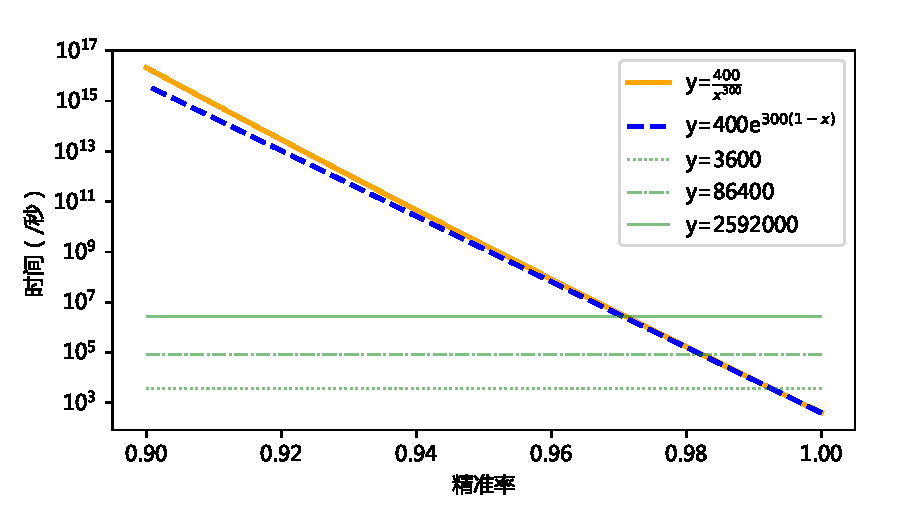
\includegraphics[width=0.8\textwidth]{expotime}
			\bicaption{\enspace \zyx 对攻击时间期望的影响}{\enspace Impact of accuracy of predicted nonce bit 0 on the expectation of attack time}
			\label{fig:expotime}
		\end{center}
	\end{figure}

	{\color{\xchange}
		
%	\tableref{tab:problemset}汇总了实施对双界面商用智能卡ECDSA实现侧信道分析时,会产生问题的根本原因。
	采集的电磁迹采样点多会导致执行DL-SCA时间长。采集的电磁迹特征点不明显、模板类攻击的攻击阶段使用基于极大似然准则的模版匹配会导致执行DL-SCA\zyx 低。电磁迹采集时间长,无法直接采集大量电磁迹,这导致深度学习模型缺少训练数据。根本原因无法解决,而执行DL-SCA时间长、\zyx 低、缺少训练数据等问题是可以通过改进DL-SCA的流程来缓解的。%以及相应的解决方案。针对选择量化指标的问题,本文从理论上说明了敏感信息泄漏估计\zyx 的合理性,并通过实验进行了验证。针对选择合理的分析技术的问题,本文使用了提出量化、去抖动、高斯模糊多种预处理技术及其组合实现POIs高效、准确地提取,使用面向基于深度学习侧信道分析的数据增强方法减少对训练数据的依赖,依据ECDSA签名实现本身的特点和采集信息泄漏的能力设定了计算敏感信息泄漏估计值的具体方案。
	%为了减少执行DL-SCA的时间、提高DL-SCA\zyx ,本文提出了\yuchuli 技术、\shujuzengqiang、\jiashejianyanguji。
	
%	\begin{table}[!h]
%		\bicaption{\enspace 导致攻击智能卡存在问题的原因}{\enspace Reasons for the existence of problems in attacking the smart card}
%		\label{tab:problemset}
%		\centering
%		\scriptsize% fontsize
%		%\setlength{\tabcolsep}{4pt}% column separation
%		%\renewcommand{\arraystretch}{1.2}%row space 
%		\begin{tabular}{c|cc}
%			\hline
%			根本原因&是否导致执行DL-SCA时间长&是否导致DL-SCA\zyx 低\\
%			\hline
%			采集的电磁迹采样点多&是&/\\
%			采集的电磁迹特征点不明显&否&是\\
%			基于极大似然准则的模版匹配&否&是\\
%			\hline
%		\end{tabular}
%		\tabnote{当电磁迹采样点多时,已经无法在可接受的时间内执行DL-SCA,因此无法获得实际\zyx 。}
%	\end{table}

	\section{基于深度学习的电磁分析方法}\label{sec:solution}
	{\color{\xchange}
		
		基于深度学习的电磁分析方法包括三个部分:\yuchuli 技术、\shujuzengqiang 和\jiashejianyanguji。它们解决了实施对双界面商用智能卡ECDSA实现侧信道分析时存在的具体难点,如\tableref{tab:solution2problem}所示。
		
		\begin{table}[!h]
			\bicaption{\enspace 技术与难点的对应关系}{\enspace Technical solutions to the problems}
			\label{tab:solution2problem}
			\centering
			\footnotesize
			%\setlength{\tabcolsep}{4pt}% column separation
			%\renewcommand{\arraystretch}{1.2}%row space 
			\begin{tabular}{cccc}
				\hline
				解决方案&是否减少执行DL-SCA时间&是否提高DL-SCA准确率 &是否增加训练数据\\
				\hline
				基于时间模板匹配&\multirow{2}{*}{是(315天$\rightarrow$8分钟)}&\multirow{2}{*}{是(无法计算$\rightarrow$91.35\%)}&\multirow{2}{*}{否}\\
				的特征点提取&&&\\
				%\hline
				\shujuzengqiang&否(8分钟$\rightarrow$1小时)&是(91.35\%$\rightarrow$95.50\%)&是\\
				%\hline
				\jiashejianyanguji&否(保持不变)&是(95.50\%$\rightarrow$100\%)&否\\
				\hline
			\end{tabular}
		\end{table}
		
	}
{

%	令$n_s=30$表示本文所采集到一条迹所包含信息泄漏所对应的的迭代次数。算法实现总共有128次迭代,但因为采集条件受限只能对连续$n_s$次迭代的信息泄漏进行采集,为了方便处理,实际数据都是采集了前$n_s$次迭代的结果。
%	
%	本文严格区分这几个概念:敏感信息、信息泄漏、信息泄漏估计值、敏感信息估计值、可利用的敏感信息估计值、被利用的敏感信息估计值。
%	
%	每条签名中,一次性随机数$\nonce$、一次性随机数的某个比特$\nonce_i$、一次性随机数编码形式中的一个码元$\tilde \nonce_i$(\algorithmref{alg:improvesignscalar}中的$\tilde\nonce_i$)都是敏感信息。攻击者不能知道敏感信息真实值,只能使用侧信道攻击或其他方法间接地估计。
%	
%	因为签名算法每次执行时这些敏感信息几乎不同,这导致算法某些步骤或数值不同,而这种不同可以在电磁迹上得以体现。\algorithmref{alg:improvesignscalar}中$\leakedmultiplier_i$是由敏感信息$\tilde\nonce_i$和随机数共同决定,$\leakedmultiplier_i$受$\tilde\nonce_i$影响,$\leakedmultiplier_i$是信息泄漏。攻击者不能知道信息泄漏的真实值。依据敏感信息和信息泄漏之间的关系,可以得到两个推论,如\corollaryref{cor:highbitinfo}和\corollaryref{cor:lowbitinfo}所示。\textbf{为了方便表述,我们将对应于$\nonce_i=0$的电磁迹称为正例,对应于$\nonce_i=1$的电磁迹称为反例。}
%	
%	攻击者获取电磁迹后,可以尝试使用侧信道攻击恢复其中的信息泄漏。因为这种恢复不能保证100\%成功,所以需要将它和信息泄漏加以区分。我们将攻击者恢复的信息泄漏称为信息泄漏估计值,记为$\hat \leakedmultiplier_i$。
%	
%	在此之后,攻击者可以依据信息泄漏估计值进一步计算敏感信息泄漏的估计值,我们将其称为敏感信息估计值。因为$\nonce,\nonce_i,\tilde \nonce_i$都是敏感信息,所以对它们各自的估计值$\hat \nonce,\hat\nonce_i,\hat{\tilde \nonce}_i$都是敏感信息估计值。本文主要对$\hat\nonce_i$进行相关的分析。具体来说,攻击者可以预先根据\corollaryref{cor:highbitinfo}和\corollaryref{cor:lowbitinfo}总结出如何根据信息泄漏估计值计算敏感信息泄漏的估计值的表格,如\apptableref{apptab:infoonsymbol}所示,每次依据信息泄漏估计值查表即可。\textbf{攻击者不知道敏感信息,因此只能暂且假设没有反例被错误预测为正例。}
%	
%	得到敏感信息估计值后,攻击者需要从中过滤出对于求解算法$\mathcal S$的可利用的敏感信息估计值。这是因为虽然有的信息泄漏带有信息但是将它交给$S$构造方程并求解反而会导致求解时间增加、求解成功率降低。对于本文使用的求解算法$S$,连续4比特$\hat \nonce_i,0\le i<n_s$的敏感信息估计值就是可利用的敏感信息估计值。
%	
%	被求解算法利用的可利用的敏感信息估计值称为被利用的敏感信息估计值。求解算法$\mathcal S$会选择一定数量\footnote{假如可利用的敏感信息估计值一定都等于真实值,那么对求解速度和求解成功率没有影响,但这种情况较难发生。如果可利用的敏感信息估计值有可能出错,那么选择越多签名就越可能含有错误,一旦有错误就会求解失败。}的签名及其可利用的敏感信息泄漏估计值构造方程并尝试求解私钥$\sk$,因此即使某些敏感信息估计值是可利用的也不会被利用。
%
%	\begin{corollary}\label{cor:highbitinfo}
%		如果$\leakedmultiplier_i=1$,那么$\nonce_i=0$。
%	\end{corollary}
%	\begin{proof}
%		证明逆否命题即可。如果$\nonce_i\neq0$,那么$\nonce_i=1$,$\tilde \nonce_i=2$或$\tilde \nonce_i=3$。当$\tilde \nonce_i=2,\leakedmultiplier_i=2\neq1$。当$\tilde \nonce_i=3,\leakedmultiplier_i=3\neq1$。因此,如果$\nonce_i\neq0$,$\leakedmultiplier_i\neq1$。
%	\end{proof}
%
%	\begin{corollary}\label{cor:lowbitinfo}
%		如果$\leakedmultiplier_i=2$,那么$\nonce_{i+129}=0$。
%	\end{corollary}
%	\begin{proof}
%		证明逆否命题即可。如果$\nonce_{i+129}\neq0$,那么$\nonce_{i+129}=1$,$\tilde \nonce_i=1$或$\tilde \nonce_i=3$。当$\tilde \nonce_i=1,\leakedmultiplier_i=1\neq2$。当$\tilde \nonce_i=3,\leakedmultiplier_i=3\neq2$。因此,如果$\nonce_{i+129}\neq0$,$\leakedmultiplier_i\neq2$。
%	\end{proof}
%	
%	\begin{example}\label{ex:rightwrongright}
%		假设对于第1337条签名中数乘算法第23、24、25、26次迭代,\algorithmref{alg:improvesignscalar}中的$\tilde\nonce_i$数值分别为$\tilde\nonce_{23}=0,\tilde\nonce_{24}=0,\tilde\nonce_{25}=1,\tilde\nonce_{26}=3$(即$\nonce_{23}=0,\nonce_{24}=0,\nonce_{25}=0,\nonce_{26}=1,\nonce_{152}=0,\nonce_{153}=0,\nonce_{154}=1,\nonce_{155}=1$)。进一步假设第23、24次迭代的随机数(\algorithmref{alg:improvesignscalar}第8行)数值分别是2、1。据此,我们可以知道电磁迹中分别包含$\leakedmultiplier_{23}=2,\leakedmultiplier_{24}=1,\leakedmultiplier_{25}=1,\leakedmultiplier_{26}=3$的信息泄漏。进一步假设攻击者通过侧信道攻击计算出了信息泄漏估计值$\hat\leakedmultiplier_{23}=1,\hat\leakedmultiplier_{24}=1,\hat\leakedmultiplier_{25}=1,\hat\leakedmultiplier_{26}=1$。尽管我们知道攻击者对$\leakedmultiplier_{23},\leakedmultiplier_{26}$做出了错误的估计,但是对于攻击者本人,他因为不知道$\leakedmultiplier_{26}$真实值而不知道已经出错,只能暂且假设估计值都是正确的。攻击者根据\apptableref{apptab:infoonsymbol},由信息泄漏估计值推算某些敏感信息估计值$\hat\nonce_{23}=0,\hat\nonce_{24}=0,\hat\nonce_{25}=0,\hat\nonce_{26}=0$。进一步发现$\hat\nonce_{23},\hat\nonce_{24},\hat\nonce_{25},\hat\nonce_{26}$是连续4比特的,所以它们是可利用的敏感信息估计值。再进一步假设攻击者在某次构造方程时选择了第1337条签名(和其他一些电磁迹)及其可利用的敏感信息泄漏估计值参与调用本文使用的求解算法$S$构造方程并求解,那么第1337条签名的$\hat\nonce_{23},\hat\nonce_{24},\hat\nonce_{25},\hat\nonce_{26}$就是被利用的敏感信息的估计值。我们知道第1337条签名中对$\nonce_{26}$估计错误会导致求解失败,但对于攻击者而言他只知道错误存在而不知道错误来自于哪一(几)处被利用的敏感信息的估计值的错误,也无法知道错误具体个数。如果攻击者在某次构造方程时没有选择了第1337条签名及其可利用的敏感信息泄漏估计值参与调用本文使用的求解算法$S$构造方程并求解,那么第1337条签名的$\hat\nonce_{23},\hat\nonce_{24},\hat\nonce_{25},\hat\nonce_{26}$就不是被利用的敏感信息的估计值。
%	\end{example}
%
%	\begin{example}
%		假设对于第2333条签名中数乘算法第17、18、19、20次迭代,\algorithmref{alg:improvesignscalar}中的$\tilde\nonce_i$数值分别为$\tilde\nonce_{17}=1,\tilde\nonce_{18}=1,\tilde\nonce_{19}=1,\tilde\nonce_{20}=1$(即$\nonce_{17}=0,\nonce_{18}=0,\nonce_{19}=0,\nonce_{20}=0,\nonce_{146}=1,\nonce_{147}=1,\nonce_{148}=1,\nonce_{149}=1$)。据此,我们可以知道电磁迹中分别包含$\leakedmultiplier_{17}=1,\leakedmultiplier_{18}=1,\leakedmultiplier_{19}=1,\leakedmultiplier_{20}=1$的信息泄漏。进一步假设攻击者通过侧信道攻击计算出了信息泄漏估计值$\hat\leakedmultiplier_{17}=1,\hat\leakedmultiplier_{18}=2,\hat\leakedmultiplier_{19}=1,\hat\leakedmultiplier_{20}=3$。尽管我们知道攻击者对$\leakedmultiplier_{18},\leakedmultiplier_{20}$做出了错误的估计,但是对于攻击者本人,他因为不知道$\leakedmultiplier_{18},\leakedmultiplier_{20}$真实值而不知道已经出错,只能暂且假设估计值都是正确的。攻击者根据\apptableref{apptab:infoonsymbol},由信息泄漏估计值推算某些敏感信息估计值$\hat\nonce_{17}=0,\hat\nonce_{147}=0,\hat\nonce_{19}=0,\hat\nonce_{149}=0$,而对于$\nonce_{146},\nonce_{18},\nonce_{148},\nonce_{20}$攻击者既没有足够大(100\%)的把握将它们估计为0,也没有足够大(100\%)的把握将它们估计为0。尽管$\hat\nonce_{17},\hat\nonce_{18},\hat\nonce_{19},\hat\nonce_{20}$是连续4比特,但是其中缺少$\hat\nonce_{18},\hat\nonce_{20}$,所以它不是可利用的敏感信息估计值。因此,它也不可能是被利用的敏感信息估计值。
%	\end{example}
%
%	\begin{example}
%		假设对于第162条签名中数乘算法第6、7、8、9次迭代,\algorithmref{alg:improvesignscalar}中的$\tilde\nonce_i$数值分别为$\tilde\nonce_{6}=2,\tilde\nonce_{7}=2,\tilde\nonce_{8}=2,\tilde\nonce_{9}=2$(即$\nonce_{6}=1,\nonce_{7}=1,\nonce_{8}=1,\nonce_{9}=1,\nonce_{135}=0,\nonce_{136}=0,\nonce_{137}=0,\nonce_{138}=0$)。据此,我们可以知道电磁迹中分别包含$\leakedmultiplier_{6}=2,\leakedmultiplier_{7}=2,\leakedmultiplier_{8}=2,\leakedmultiplier_{9}=2$的信息泄漏。进一步假设攻击者通过侧信道攻击计算出了信息泄漏估计值$\hat\leakedmultiplier_{17}=2,\hat\leakedmultiplier_{18}=2,\hat\leakedmultiplier_{19}=2,\hat\leakedmultiplier_{20}=2$。攻击者根据\apptableref{apptab:infoonsymbol},由信息泄漏估计值推算某些敏感信息估计值$\hat\nonce_{135}=0,\hat\nonce_{136}=0,\hat\nonce_{137}=0,\hat\nonce_{138}=0$。进一步发现$\hat\nonce_{135},\hat\nonce_{136},\hat\nonce_{137},\hat\nonce_{138}$是连续4比特,它因为其索引不在区间[0,$n_s$)而不可能被本文的求解算法$S$利用,所以它不是可利用的敏感信息估计值。因此,它也不可能是被利用的敏感信息估计值。
%	\end{example}
%
%	本文严格区分攻击者和分析者,这是因为两者能力范围有所差异。只从攻击者角度看待问题会导致无法获取分析性能所需的必要的信息,只从评估者角度看待问题会导致攻击方法有可能会依赖于只有评估者才能获取的信息,从而不能用于实际攻击。
%
%	对于攻击者,他不知道攻击电磁迹所对应的敏感信息,也不知道信息泄漏。攻击者的攻击路线是:根据电磁迹计算信息泄漏估计值、在假设信息泄漏估计值完全正确的情况下计算敏感信息估计值、从敏感信息估计值中计算求解算法$\mathcal S$可利用的敏感信息估计值、选出对于$\mathcal S$来说足够多的可利用的敏感信息估计值并结合签名本身的一些公开内容构造方程调用$\mathcal S$并求解私钥、验证求解结果。如果攻击者验证出求解结果错误,只能说明攻击路线中恰好遇到“信息泄漏估计值完全正确”不成立的情况且有错误一直保留到了最后阶段,但没有办法进一步确认错误来自于“足够多被利用的信息泄漏估计值”中的哪一处或哪几处。
%
%	对于分析者,它相比于攻击者可以额外知道电磁迹所对应的敏感信息,但是信息泄漏的真实值也不能全部知道(见\tableref{tab:partialknownticonclusion},大约只能知道所有信息泄漏中$\frac34$的比例)。从分析者角度可以依据这个信息计算出攻击者求解结果错误时,错误来自于“足够多被利用的信息泄漏估计值”中的哪一处或哪几处。因为分析者不能全不知道信息泄漏的真实值,所以只能定位一些错误而不是所有错误。例如,在\exampleref{ex:rightwrongright}中,评估者实际上也无法知道第1337条签名中数乘算法第23次迭代的信息泄漏真实值$\leakedmultiplier_{23}=2$与信息泄漏估计值$\hat\leakedmultiplier_{23}=1$是不一致的。

%	本文严格区分这几个概念:成功率(Success Rate)、准确率(Accuracy)、精确率(Precision)。
%	
%	成功率用于描述求解算法$\mathcal S$,$\mathcal S$是一个近似算法因此即使构造的方程不含错误它也不能保证100\%求解成功。因为$\mathcal S$的成功率难以估计且$\mathcal S$并不在本文研究范围内,本文直接假定$\mathcal S$成功率为100\%。
%	
%	准确率用于描述信息泄漏$\leakedmultiplier_i$的恢复情况。$\leakedmultiplier_i$可能的取值有三种,因此使用DL-SCA预测标签是一个三分类问题。它的混淆矩阵如\tableref{tab:cmatrixt}所示。恢复信息泄漏$\leakedmultiplier_i$准确率的计算方式为$accuracy=\frac{\mathrm{TP}1+\mathrm{TP}2+\mathrm{TP}3}{\mathrm{TP}1+\mathrm{FP}1_2+\mathrm{FP}1_3+\mathrm{FP}2_1+\mathrm{TP}2+\mathrm{FP}2_3+\mathrm{FP}3_1+\mathrm{FP}3_2+\mathrm{TP}3}$,它是深度学习最常用的评价指标。
%
%	精确率用于描述敏感信息$\nonce_i$的恢复情况。$\nonce_i$可能的取值有只有两种,因此使用DL-SCA预测标签是一个二分类问题。它的混淆矩阵如\tableref{tab:cmatrixk}所示。恢复敏感信息$\nonce_i$的精确率的计算方式如\equationref{eq:precision}所示,它适用于不能容忍将反例错误预测为正例的情况。
%
%	\begin{equation}\label{eq:precision}
%		precision=\frac{TP}{TP+FP}
%	\end{equation}
%
%	在侧信道领域,通常使用准确率描述敏感信息恢复情况。恢复敏感信息$\nonce_i$的准确率计算方式为$accuracy=\frac{TP+TN}{TP+FP+FN+TN}$。\textbf{但是},恢复敏感信息$\nonce_i$的准确率这一指标在对ECDSA实现的侧信道分析研究场景中存在缺陷。本文只论证其缺陷,不会将恢复敏感信息$\nonce_i$的准确率用作评价指标。
%
%	\begin{table}[!h]
%		\bicaption{\enspace $\leakedmultiplier_i$的混淆矩阵}{\enspace Confusion matrix of $\leakedmultiplier_i$}
%		\label{tab:cmatrixt}
%		\centering
%		%\footnotesize% fontsize
%		%\setlength{\tabcolsep}{4pt}% column separation
%		%\renewcommand{\arraystretch}{1.2}%row space
%		\begin{tabular}{cc|ccc}
%			\hline
%			\multicolumn{2}{c|}{\multirow{2}{*}{样本数}} & \multicolumn{3}{c}{$\hat\leakedmultiplier_i$的取值(预测结果)} \\
%			%\cline{3-5}
%			\multicolumn{2}{c|}{}& 1 & 2 & 3 \\
%			\hline
%			\multirow{3}{*}{$\leakedmultiplier_i$的取值(真实结果)} & 1 & TP1 & FP1$_2$ & FP1$_3$ \\
%			%\cline{2-5}
%			& 2 & FP2$_1$ & TP2 & FP2$_3$ \\
%			%\cline{2-5}
%			& 3 & FP3$_1$ & FP3$_2$ & TP3 \\
%			\hline
%		\end{tabular}   
%	\end{table}
%
%	\begin{table}[!h]
%		\bicaption{\enspace $\nonce_i$的混淆矩阵}{\enspace Confusion matrix of $\nonce_i$}
%		\label{tab:cmatrixk}
%		\centering
%		%\footnotesize% fontsize
%		%\setlength{\tabcolsep}{4pt}% column separation
%		%\renewcommand{\arraystretch}{1.2}%row space
%		\begin{tabular}{cc|cc}
%			\hline
%			\multicolumn{2}{c|}{\multirow{2}{*}{样本数}} & \multicolumn{2}{c}{$\hat\nonce_i$的取值(预测结果)} \\
%			%\cline{3-5}
%			\multicolumn{2}{c|}{}& 0& 1 \\
%			\hline
%			\multirow{2}{*}{$\nonce_i$的取值(真实结果)} & 0 & TP & FP \\
%			%\cline{2-5}
%			& 1 & FN & TN \\
%			\hline
%		\end{tabular}   
%	\end{table}
%
%	ECDSA签名过程使用的一次性随机数$\nonce$是敏感信息。如果它出现泄漏,那么攻击者有可能使用数学方法恢复私钥$\sk$。随机数$\nonce$泄漏越多,攻击恢复私钥的可能性越大。
%	
%	对于本文研究的双界面商用智能卡ECDSA实现,不能直接使用侧信道攻击恢复一次性随机数$\nonce$的泄漏。如\algorithmref{alg:improvesignscalar}所示,算法的敏感信息是$\tilde{\nonce}_i,i=0,1,\cdots, 128$,但它不存在泄漏(或泄漏程度小到不能直接利用)。我们注意到$\leakedmultiplier_i$与敏感信息有关(\algorithmref{alg:improvesignscalar}第5行)且它存在可以利用的泄漏,因此可以将攻击点选为$\leakedmultiplier_i$,预测$\leakedmultiplier_i$的估计值$\hat\leakedmultiplier_i$后,可以预测某些$\nonce_i$的估计值$\hat\nonce_i$。
%	
%	\begin{figure}[!h]
%		\begin{center}
%			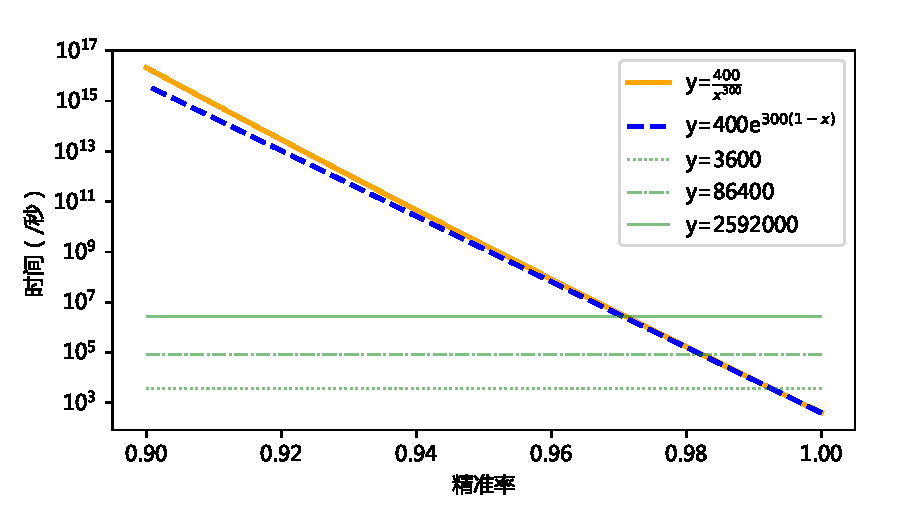
\includegraphics[width=\textwidth]{expotime}
%			\bicaption{\enspace 敏感信息估计值精确率对攻击时间期望的影响}{\enspace Impact of precision on the expectation of attack time}
%			\label{fig:expotime}
%		\end{center}
%	\end{figure}
%	
%	需要注意的是,求解算法$\mathcal S$要求\textbf{被利用的敏感信息估计值}的准确率是100\%,而没有要求\textbf{可利用的敏感信息估计值}准确率是100\%。又由于\corollaryref{cor:highbitinfo}和\corollaryref{cor:lowbitinfo},我们可以知道\textbf{可利用的敏感信息估计值}都是被预测为正例的\footnote{三段论。大前提,敏感信息都被预测为正例。小前提,可利用的敏感信息估计值是敏感信息。结论,可利用的敏感信息估计值都被预测为正例。}。既然所有\textbf{可利用的敏感信息估计值}都是被预测为正例的,那么\textbf{可利用的敏感信息估计值}的准确率就是精确率。又由于\textbf{可利用的敏感信息估计值}在\textbf{所有预测为正例的敏感信息估计值}中的分布是随机的,因此\textbf{可利用的敏感信息估计值}的准确率约等于\textbf{所有预测为正例的敏感信息估计值}的准确率,即\textbf{敏感信息估计值}精确率。
%	
%	因此,在敏感信息估计值精确率略小于100\%的情况下,可以多次尝试仅使用部分泄漏并使用$S$求解。如果选取到的部分泄漏恰好没有错误,那么求解算法能求解出实际私钥$\sk$。这样带来的代价是需要消耗更多时间才能恢复实际私钥。具体来讲,在敏感信息估计值精确率略小于100\%的情况下,使用多次尝试$S$的方法所消耗的时间会随着精确率的减小而成指数级增长,推导过程如\propositionref{prop:expotime}所示。\figureref{fig:expotime}展示了敏感信息估计值精确率略小于100\%的情况下多次尝试$S$的方法在理论上的技术效果,其中橙色实线表示恢复实际私钥的时间的期望,蓝色虚线表示使用指数函数可以对时间期望的下限做一个很好的估计,不同线型的绿色虚线表示攻击所能容忍的不同程度时间消耗(一小时、一天、一个月)。进一步分析可以知道,如果要求使用数学方法分别在一个月、一天、一小时内恢复实际私钥,那么通过侧信道攻击所恢复敏感信息估计值精确率分别需要达到97.12\%、98.22\%、99.27\%。
%
%	本文的攻击点是ECDSA签名操作中数乘实现(\algorithmref{alg:improvesignscalar})中$\leakedmultiplier_i$的泄漏,侧信道攻击最终目标是恢复足够多可利用\footnote{足够多、可利用的具体标准取决于求解算法$\mathcal S$。对于本文使用的求解算法$S$,足够多指使用75条有可利用泄漏的签名构造方程,可利用指签名中的随机数泄漏连续4比特。}的签名中的一次性随机数$\nonce$的泄漏的情况下,提高敏感信息估计值精确率。侧信道攻击恢复敏感信息估计值精确率越高,求解实际私钥所需要调用$S$的次数就越少,攻击时间也就越少。侧信道攻击恢复随机数泄漏越多,求解出实际私钥的可能性就越大。

%	侧信道攻击智能卡ECDSA直到恢复实际私钥分为如下多个步骤。其中,步骤一可以通过改进采集环境或采集设备提升采集到的泄漏数量,步骤二通过改进侧信道攻击方法或降低置信度提升恢复的信息泄漏数量,步骤三需要通过更强的数学工具才可能在现有基础(见\apptableref{apptab:infoonsymbol})上进一步提升恢复敏感信息泄漏的比例,步骤四无法改进,步骤五可以通过使用更好的求解算法加以改进以减少攻击时间。
%	
%	\begin{enumerate}
%		\item [\textbf{步骤一}]采集多条签名以及对应的电磁迹;
%		\item [\textbf{步骤二}]从电磁迹中预测信息泄漏$\leakedmultiplier_i$的估计值$\hat \leakedmultiplier_i$;
%		\item [\textbf{步骤三}]从信息泄漏估计值$\hat \leakedmultiplier_i$计算某些敏感信息的估计值$\hat \nonce_i$;
%		\item [\textbf{步骤四}]从签名中过滤出所有有连续4比特泄漏的签名;
%		\item [\textbf{步骤五}]每次随机选择75条签名,利用签名以及其泄漏调用$S$求解直至求解成功。
%	\end{enumerate}
%	
%	对于步骤一,在现有实验条件下(见\tableref{tab:acquisitionpara})每条签名中数乘实现时长约50ms的电磁迹只能采集10ms,128次迭代只能采集到约30次(即$n_s\approx30$)。对于步骤二,使用通用数据增强方法提升恢复的信息泄漏数量。步骤三、四、五不在本文范围内,提升效果的具体方法不予赘述。
%	
%	本文不考虑进一步改进步骤一、三、四、五,这使得使用侧信道分析实现步骤二需要考虑如下难点:
%	
%	\begin{itemize}
%		\item 信息泄漏难以定位;
%		\item 敏感信息估计值精确率要求高\footnote{具体数值由电磁迹条数、电磁迹包含的迭代次数、从信息泄漏中恢复敏感信息泄漏的比例、求解算法$\mathcal S$对可利用敏感信息泄漏的定义、求解算法$\mathcal S$对敏感信息泄漏总量的需求、求解算法$\mathcal S$的运行时间、求解算法$\mathcal S$本身的成功率、可以容忍的攻击的时间消耗等多种因素共同决定。};
%	\end{itemize}

%	\subsection{量化指标选择}
%	
%	针对量化指标选择的问题,本文使用了\zyx 作为评价指标,计算方式如\equationref{eq:tpr}所示。本文将敏感信息泄漏值$\nonce^{(i)}_j=0,i=0,1,\dots,T_a-1,j=0,1,\dots,n_s-1$的样本称为阳性样本,$\nonce^{(i)}_j=1,i=0,1,\dots,T_a,j=0,1,\dots,n_s-1$的样本称为阴性样本。据此可以定义真阳性、真阴性、假阳性、假阴性的样本。
%	
%	\begin{itemize}
%		\item [真阳性] 如果样本符合$\nonce^{(i)}_j=0,\hat \nonce^{(i)}_j=0$的条件,那么它是真阳性;
%		\item [真阴性] 如果样本符合$\nonce^{(i)}_j=1,\hat \nonce^{(i)}_j=1$的条件,那么它是真阴性;
%		\item [假阳性] 如果样本符合$\nonce^{(i)}_j=1,\hat \nonce^{(i)}_j=0$的条件,那么它是假阳性;
%		\item [假阴性] 如果样本符合$\nonce^{(i)}_j=0,\hat \nonce^{(i)}_j=1$的条件,那么它是假阴性。
%	\end{itemize}
%
%	\begin{equation}\label{eq:tpr}
%		TPR=\frac{TP}{TP+FP}
%	\end{equation}
%
%	在此基础上,本文将真阳性、真阴性、假阳性、假阴性样本的样本个数分别记为TP、TN、FP、FN,它们的关系如\tableref{tab:cmatrixk}所示。\zyx 的计算方式如\equationref{eq:tpr}所示,它适用于不能容忍将阴性样本错误估计为阳性的情况。就本文而言,因为ECDSA本身的特性以及后续格方法的特殊要求,假阴性的数量或比例在不超过阈值的情况下不会对求解私钥的效率和正确性产生影响,证明见\propositionref{prop:highalpha}。因此,虽然\zyx 作为评价指标的场景少见,但它适合作为本文评价指标。
%
%	\begin{table}[!h]
%		\bicaption{\enspace $\nonce_j$的混淆矩阵}{\enspace Confusion matrix of $\nonce_j$}
%		\label{tab:cmatrixk}
%		\centering
%		%\footnotesize% fontsize
%		%\setlength{\tabcolsep}{4pt}% column separation
%		%\renewcommand{\arraystretch}{1.2}%row space
%		\begin{tabular}{c|c|cc}
%			\hline
%			\multicolumn{2}{c|}{\multirow{2}{*}{样本数}} & \multicolumn{2}{c}{$\hat \nonce^{(i)}_j$(估计值)} \\
%			\cline{3-4}
%			\multicolumn{2}{c|}{}& 0& 1 \\
%			\hline
%			\multirow{2}{*}{$\nonce^{(i)}_j$(值)} & 0 & TP & FP \\
%			%\cline{2-5}
%			& 1 & FN & TN \\
%			\hline
%		\end{tabular}   
%	\end{table}
}
	
	%\subsection{分析技术选择}
	\subsection{ECDSA电磁迹预处理}\label{subs:selectpoi}

	直接使用深度学习模型对电磁迹进行DL-SCA在理论上可行,但是在实践中所需的计算量巨大,本文实验环境需要使用315天才能完成深度学习模型的训练。为了解决这个问题,本文选择从提取POIs的角度实现预处理,提出了\poifanwei 和\yuchuli 技术,在尽可能保留特征的同时减少信息泄漏的维数,对应的深度学习模型所需的存储空间和训练的计算量可以有效地减小,使用现有的计算资源足够进行DL-SCA。这样做还带来一个额外的好处:电磁迹可以根据POIs对齐结果,量化评价对齐程度可以直观地反映特征点提取是否准确。
{	
%	本文提出了一种基于时间模板的两阶段对齐解决信息泄漏难以定位的问题;本文应用了前一章的通用数据增强方法提升敏感信息估计值精确率。
	
%	侧信道分析的第一个难点在于,敏感信息是$\tilde{k}_i$没有直接泄漏,这使得从理论上讲不可能从电磁迹泄漏中恢复所有敏感信息。从一条签恢复的恢复的敏感信息越少,就需要使用越多签名构造方程才可能求解出私钥。
%	
%	
%	即使以100\%的成功率恢复所有泄漏的$t_i$,也会因无法分辨泄漏来自于算法的哪个分支(\algorithmref{alg:improvesignscalar}第5、8行),从而在理论上不能完全恢复$\tilde k_i$的信息,进而不能恢复随机数$k$的所有泄漏\footnote{因为$\left\{\tilde{k}_0,\tilde{k}_1,\dots,\tilde{k}_i,\dots, \tilde{k}_{l-1}\right\}$是$k$的编码形式,所以恢复某些$\tilde k_i$的比特等价于恢复随机数$k$的等量比特。因为$(k_0k_1k_3\dots k_{257})_2$是$k$的二进制表示,所以恢复某些$k_i$也等价于恢复随机数$k$的等量比特。}。\tableref{tab:infoonsymbol}总结了从$t_i$中所恢复的$\tilde k_i$和$k$的信息。从\tableref{tab:infoonsymbol}中可以归纳出这样的结论:
%	
%	\begin{itemize}
%		\item 如果攻击者知道$t_i=1$(有$\frac38$的概率发生),那么攻击者可以推断$\tilde k_i$的高比特是0,即$k_i=0$(见\algorithmref{alg:encodek}),无法推断$\tilde k_i$的低比特。
%		\item 如果攻击者知道$t_i=2$(有$\frac5{16}$的概率发生),那么攻击者可以推断$\tilde k_i$的低比特是0,即$k_{i+129}=0$,无法推断$\tilde k_i$的高比特。
%		\item 如果攻击者知道$t_i=3$(有$\frac5{16}$的概率发生),那么攻击者无法推断$\tilde k_i$的任意比特。
%	\end{itemize}
%	
%	
%	侧信道攻击所能恢复的是$t_i$的数值,构造方程的签名中的随机数泄漏是$\tilde k_i$的数值,这两个不能完全对应。依据前两条结论从$t_i$中推断出的随机数$k$的某些比特的值就是攻击者可以完全确定的所有随机数$k$的泄漏。这些泄漏随机地分布在随机数$k$所有位置。因此攻击者
%		
%	从\tableref{tab:infoonsymbol}中归纳的信息可以看出,对于任意一条签名中随机数$k$的任意一个比特$k_i$,不可能使用侧信道攻击得出这样的结论:有超过100\%的把握认为$k_i=1$。
%	
%	实际上,在采集的电磁迹受限的情况下,侧信道攻击恢复随机数泄漏多和侧信道攻击恢复随机数泄漏的准确率高两个目标是互相冲突的。原因在于,在采集的电磁迹受限下,可以很容易地通过提高置信度实现提高侧信道攻击恢复随机数泄漏的准确,但是这样一来会减少侧信道攻击恢复随机数泄漏。
	
	
%	\section{智能卡ECDSA算法实现信息泄漏预处理方法研究}
%	%$\forall 0\le i<T,\forall 0\le j<n_s\leakedmultiplier^{(i)}_j$估计值$\hat\leakedmultiplier^{(i)}_j$的泄漏是信息泄漏。$\forall 0\le i<T,\forall 0\le j<n_s,\tilde \nonce^{(i)}_j,\nonce^{(i)}_j,\nonce^{(i)}_{j+129},\mathbb 1_{\leakedmultiplier^{(i)}_j=1}$数值的泄漏是信息泄漏,其中$\mathbb 1$是示性函数,取值范围为0或1,它取1当且仅当下标表示的事件发生。可利用的敏感信息指的是$\tilde \nonce_i,0<i<258$数值的泄漏
%	
%	%//TODO:
%	侧信道攻击需要预测敏感信息的准确率高,但是对于以准确率作为评价恢复信息泄漏$\leakedmultiplier_i$效果的指标不合理。从\apptableref{apptab:infoonsymbol}可以看出攻击者只能从$\hat\leakedmultiplier_i$的取值中对一次性随机数$\nonce$的某个比特$\nonce_i$做出$\hat\nonce_i=0$的估计,而无法对任意比特做出$\hat\nonce_i=1$的估计。因此评价恢复$\leakedmultiplier_i$信息泄漏效果时,只用考虑在预测$\hat\leakedmultiplier_i=1$的条件下尽可能达成$\leakedmultiplier_i=1$、预测$\hat\leakedmultiplier_i=2$的条件下尽可能达成$\leakedmultiplier_i=2$,而不用考虑在预测$\hat\leakedmultiplier_i=3$的条件下尽可能达成$\leakedmultiplier_i=3$。为了方便,我们用\tableref{tab:cmatrixt}所列举的表项说明这种变化,评价指标由$accuracy=\frac{\mathrm{TP}1+\mathrm{TP}2+\mathrm{TP}3}{\mathrm{TP}1+\mathrm{FP}1_2+\mathrm{FP}1_3+\mathrm{FP}2_1+\mathrm{TP}2+\mathrm{FP}2_3+\mathrm{FP}3_1+\mathrm{FP}3_2+\mathrm{TP}3}$变为$\frac{\mathrm{TP}1+\mathrm{TP}2}{\mathrm{TP}1+\mathrm{FP}1_2+\mathrm{FP}2_1+\mathrm{TP}2+\mathrm{FP}3_1+\mathrm{FP}3_2}$。又由于本文使用的求解算法$S$不考虑低位的泄漏,因此本文只考虑在预测$\hat\leakedmultiplier_i=1$的条件下尽可能达成$\leakedmultiplier_i=1$。我们还是用\tableref{tab:cmatrixt}所列举的表项说明这种变化,评价指标由$\frac{\mathrm{TP}1+\mathrm{TP}2}{\mathrm{TP}1+\mathrm{FP}1_2+\mathrm{FP}2_1+\mathrm{TP}2+\mathrm{FP}3_1+\mathrm{FP}3_2}$进一步变为$\frac{\mathrm{TP}1}{\mathrm{TP}1+\mathrm{FP}2_1+\mathrm{FP}3_1}$。根据\corollaryref{cor:highbitinfo}可以知道,\tableref{tab:cmatrixt}所列举的表项表述的公式$\frac{\mathrm{TP}1}{\mathrm{TP}1+\mathrm{FP}2_1+\mathrm{FP}3_1}$实际上就是\tableref{tab:cmatrixk}所列举的表项表述的\equationref{eq:precision}。因此我们将$\frac{\mathrm{TP}1}{\mathrm{TP}1+\mathrm{FP}2_1+\mathrm{FP}3_1}$称为信息泄漏估计值$\hat\leakedmultiplier_i$的精确率,它和敏感信息估计值$\hat\nonce_i$的精确率在数值上是恒等的。
%	
%	信息泄漏指的是$\leakedmultiplier_i$的泄漏。
}
	
	通常来说,提取POIs是通过对电磁迹进行对齐,再从对齐结果中选取POIs。但就本文而言,一条签名的电磁迹采样点个数达到5000万,但一条电磁迹中包含150小组、共7500个特征不明显的POIs,且不同组的50个POIs不连续。现有的对齐方法无法同时满足高效和准确的需求,因此也不能高效和准确的完成POIs的提取。电磁迹中每处信息泄漏的POIs少(约50个采样点),使用基于与单处信息泄漏相关系数的静态对齐会因为产生大量误报\footnote{原本不存在敏感信息泄漏,但是静态对齐结果显示存在敏感信息泄漏。}而无法准确提取POIs。电磁迹中每处信息泄漏之间引入了随机延迟,使用基于与多处信息泄漏相关系数的静态对齐会使得出现大量漏报\footnote{原本存在敏感信息泄漏,但是静态对齐结果显示不存在敏感信息泄漏。}而过滤掉可利用的信息泄漏。电磁迹中每处信息泄漏间隔的时间长,使用动态对齐会因为计算量巨大而不能高效提取POIs。
	
	本文提出\yuchuli 技术。它的核心思想是筛选电磁迹和卷积核卷积的极值点\footnote{极大值点或极小值点。在一个有定义的点的周围的点也都有定义,且在这个点的左右邻域的函数值都小于这个点的值,则该点为极大值点,同理为极小值点。},将最匹配时间模板的极值点组合记为POIs。
%	本文提出一种基于时间模板的\yuchuli 预处理技术可以高效准确地从目标电磁迹中提取POIs。它大致分为如下两个阶段:
%	
%	\begin{itemize}
%		\item [\textbf{阶段一,高效确定信息泄漏范围}]分块计算方差,对分块结果依次进行模数转换、去抖动、一维高斯模糊、模数转换、去抖动,定位到泄漏的大致范围,将电磁迹初步划分为电磁子迹;
%		\item [\textbf{阶段二,准确确定信息泄漏位置}]在电磁子迹中计算不同偏移程度下与一处信息泄漏的模板的协方差,筛选出一定数量的极值点,枚举可能极值点的组合检查是否匹配信息泄漏的时间模板。
%	\end{itemize}
	在执行\yuchuli 之前,需要使用分块方差以及模数转换、去抖动、一维高斯模糊的信号处理技术缩小POIs范围,提高\yuchuli 效率。\yuchuli 之前的这个预计算操作称为\poifanwei 技术。
	
	
	%可以认为智能卡ECDSA算法实现信息泄漏预处理的时间消耗和采样点个数线性相关。在阶段一,本文在保留信息泄漏特征的情况下使用时间复杂度低($\Theta(M)$)的算法高效确定信息泄漏范围;在阶段二,本文使用时间复杂度高($\Theta(n_sM_s\log M_s)$)的算法准确确定信息泄漏位置。算法复杂度中的$M,n_s,M_s$分别表示电磁迹采样点个数、电磁迹包含的迭代次数、一次迭代所对应的电磁子迹\footnote{本文将一次迭代所对应的POI附近的电磁迹称为电磁子迹(Subtrace)的采样点个数,这么命名的原因是它实际上就是电磁迹的一部分。}的采样点个数。虽然阶段二的算法复杂度较高,但是算法复杂度中的变量的数值更小(对于本文,$M=5\cdot10^7,n_s=30,M_s=18000$),所以在当前数据范围内阶段二时间消耗也是很小的。因此,预处理时间消耗中执行阶段一的时间消耗占主导作用,预处理时间消耗和电磁迹采样点个数线性相关。

	\textbf{采用\poifanwei 技术确定特征点范围。}	
	\poifanwei 技术使用降采样的思想,以线性时间复杂度定位到POIs的大致范围,范围从5000万采样点减小到1.8万采样点。一条5000万个采样点的电磁迹含有30组POIs,每组POIs互不连续(坐标之差超过一百万采样点),一组POIs包括5小组不连续的POIs(每个POI与同组的其他POI的距离在2300至3500采样点之间)。\poifanwei 技术首先依据信息泄漏部分电磁场强度变化大的特性分块计算方差可以降采样并使得信息泄漏处依然保留的特征。接着依次使用模数转换、去抖动、模糊、模数转换、去抖动的方法组合电磁迹更多信息得到的用于确定特征点范围的辅助信息。这个辅助信息是一个01数列,我们将其视为方波的采样结果。此时电磁迹可以依据计算出的辅助信息较为准确地划分每次迭代\footnote{具体划分方法取决于模数转换、去抖动、一维高斯模糊、模数转换、去抖动的参数。对于本文的电磁迹和函数参数,每过8个方波,数乘实现会在上升沿进入下一次迭代。},且每次迭代中有多个锚点辅助定位泄漏的大致范围\footnote{锚点即为方波的上升沿或下降沿时刻。对于本文的电磁迹和函数参数,每次迭代中第一个方波的下降沿到泄漏的位置相隔的采样点个数一定在区间$[8.0\cdot10^{4},9.8\cdot10^{4}]$以内。}。
	
	分块方差的实现见\algorithmref{alg:calcvar},它依据参数$w_d$对电磁迹分块并计算每块中所有电磁场强度样本值的方差,在信息泄漏处依然保留的特征的情况下进行降采样以降低后续操作的时间复杂度,其本身时间复杂度$\Theta(M)$。分块计算方差的输出结果可以视为一个降采样后的波。
	
	\begin{breakablealgorithm}
		\caption{分块方差}\label{alg:calcvar}
		\begin{algorithmic}[1]
			\Statex \textbf{输入:} $\Vector{l}^{(i)}$:采样点个数为$M$的电磁迹
			\Statex \textbf{输入:} $w_d$:分块大小
			\Statex \textbf{输出:} $\Vector D$:分块后每块的方差
			\For {$j:=0,\dots,\left\lfloor\frac{M}{w_d}\right\rfloor-1$}
			\State $d_i:=\mathrm{Var}(l^{(i)}_{jw_d},l^{(i)}_{jw_d+1},\dots,l^{(i)}_{jw_d+w_d-1})$
			\EndFor
			\State \Return $\left\{d_0,d_1,\dots,d_{\left\lfloor\frac{M}{w_d}\right\rfloor-1}\right\}$
		\end{algorithmic}
	\end{breakablealgorithm}
	
	模数转换的实现见\algorithmref{alg:quantize},它依据阈值参数$th$将非01数列(模拟信号)转换为01数列(数字信号)以便于后续操作和分析,其时间复杂度为$\Theta(N_X)$。
	
	\begin{breakablealgorithm}
		\caption{模数转换}\label{alg:quantize}
		\begin{algorithmic}[1]
			\Statex \textbf{输入:} $\Vector X$:采样点个数为$N_X$的数列
			\Statex \textbf{输入:} $th$:模数转换的阈值
			\Statex \textbf{输出:} $\Vector Q$:模数转换后的数列
			\For {$i:=0,\dots, N_X-1$}
			\If{$x_i<th$}
			\State $q_i:=0$
			\Else
			\State $q_i:=1$
			\EndIf
			\EndFor
			\State \Return $\left\{q_0,q_1,\dots,q_{N_X-1}\right\}$
		\end{algorithmic}
	\end{breakablealgorithm}
	
	本文从硬件设计中对物理按键去抖动的硬件代码得到启发而设计了去抖动函数。函数通过缓存一段长度的数列实现排除偶然噪声(采样点个数少于$w_a$的方波)的干扰但保留主体波形,它的实现见\algorithmref{alg:antijitter}。它通过检查当前位置数据以及之前的$w_a-1$个数据,综合判断应该如何解析当前状态并记录。去抖动会对数据引入延迟,去抖动后方波的上升沿和下降沿会相比于去抖动前延后$w_a$个采样点,有时需要进行校正。去抖动时间复杂度为$\Theta(N_X)$。
	
	\begin{breakablealgorithm}
		\caption{去抖动}\label{alg:antijitter}
		\begin{algorithmic}[1]
			\Statex \textbf{输入:} $\Vector X$:采样点个数为$N_X$的01数列
			\Statex \textbf{输入:} $w_a$:去抖动窗口大小
			\Statex \textbf{输出:} $\Vector A$:去抖动后的数列
			\State $s:=0$\Comment{初始状态需要设置为常数,可以是0,也可以是1}
			\State $b:=0$
			\For {$i:=0,\dots, N_X-1$}
			\State $b:=(b\cdot2+x_i)\bmod 2^{w_a}$
			\If{$b=0$}
			\State $s:=0$\Comment{连续$w_a$比特0需要重置状态为0}
			\ElsIf {$b=2^{w_a}-1$}
			\State $s:=1$\Comment{连续$w_a$比特1需要设置状态为1}
			\EndIf
			\State $a_i:=s$
			\EndFor
			\State \Return $\begin{bmatrix}a_0&a_1&\ldots&a_{N_X-1}\end{bmatrix}$
		\end{algorithmic}
	\end{breakablealgorithm}
	
	本文从图像处理中的模糊操作得到启发而设计了模糊函数。函数计算窗口大小为$2w_g+1$的二项分布的卷积核,扫描数列中的每个样本,用卷积核确定的邻域内的样本的加权平均数替代当前样本的值,它的实现见\algorithmref{alg:gaussblur}。它作为上一步去抖动函数的补充,进一步排除噪声的干扰并保留主体波形。模糊函数本质上是实现了卷积,为了使得模糊后的数列与输入的数列大小相同,卷积使用了same\footnote{使用文档见\href{https://numpy.org/doc/stable/reference/generated/numpy.convolve.html}{numpy.convolve}。}模式。模糊函数的时间复杂度为$\Theta(w_gN_X)$。
	
	\begin{breakablealgorithm}
		\caption{模糊}\label{alg:gaussblur}
		\begin{algorithmic}[1]
			\Statex \textbf{输入:} $\Vector X$:采样点个数为$N_X$的数列(下标范围之外的数值为0)
			\Statex \textbf{输入:} $w_g$:高斯模糊的窗口大小的一半(下取整)
			\Statex \textbf{输出:} $\Vector G$:高斯模糊的数列
			\For {$i:=0,\dots, 2w_g$}
			\State $c_i:=\begin{pmatrix}
			2w_g\\
			i
			\end{pmatrix}$\Comment{组合数}
			\EndFor
			\State $Kernel:=2^{-2w_g}\begin{bmatrix}c_0&c_1&\ldots&c_{2w_g}\end{bmatrix}$\Comment{计算卷积核}
			\State $\Vector G=Kernel*X$\Comment{卷积}
			%			\For {$i:=0\dots N_X-1$}
			%			\State $g_i:=K\cdot [x_{i-w_g},x_{i-w_g+1},\dots,x_{i+w_g-1},x_{i+w_g}]$
			%			\EndFor
			\State \Return $G$%$\left\{g_0,g_1,\dots,g_{N_X-1}\right\}$
		\end{algorithmic}
	\end{breakablealgorithm}
	
	执行模糊操作之后,需要再次执行模数转换和去抖动,利用这之后的结果才能确定特征点范围。

	\poifanwei 最耗费时间的是模糊操作。如果不进行分块那么$N_X=M$,它的时间复杂度$\Theta(w_gN_X)=\Theta(w_gM)$是难以接受的。分块计算方差后,每条电磁迹长度为$M$的采样点被压缩成了长度为$N_X=\left\lfloor\frac{M}{w_d}\right\rfloor$的数列,模糊的时间复杂度下降为$\Theta(w_gN_X)=\Theta(\frac{w_g}{w_d}M)$。只要$w_g<w_d$,\poifanwei 的时间复杂度就可以由$\Theta\left( w_gM\right) $变为$\Theta(M)+\Theta\left( \frac{M}{w_d}\right) +\Theta\left( \frac{M}{w_d}\right) +\Theta\left( \frac{w_g}{w_d}M\right) +\Theta\left( \frac{M}{w_d}\right) +\Theta\left( \frac{M}{w_d}\right) =\Theta(M)$。对于本文,$M=5\cdot10^7,w_d=360,w_g=300$。
	
	通过应用\poifanwei 技术,可以完全确定电磁迹30组POIs中,每组POIs都在长度为18000个采样点的区间内。%此时对$n_s$次迭代中包含信息泄漏的电磁迹进行subsub基于与单处信息泄漏相关系数的静态对齐,还是不能保证5处包含信息泄漏的电磁迹会恰好对应相关系数的前五个极值点。
	
	%本文在前一个阶段最后步骤上改动了两个实现细节以实现阶段二,一个是计算相关系数改为计算协方差,另一个是将取前5个相关系数极值点改为取前$m$个相关系数极值点,枚举其中的5个并逐一使用实现构造的时间模板进行检查。
	
	%计算协方差而不是相关系数的原因是,信息泄漏对应的电磁场变化幅度较大,但是计算相关系数会丢弃这种特征。使用协方差就是在使用相关系数的基础上一并考虑了信息泄漏电磁迹本身的方差,因此使得信息泄漏更容易被区分。除此之外,将相关系数改为计算协方差后,只要模板的所有点的均值为0,计算所有采样点邻域的相关系数就可以直接用卷积实现,这可以减少程序的时间消耗。计算协方差的算法复杂度是$\Theta(w_tN_X)$,其中$w_t$是模板宽度,$N_X$是信息泄漏所在区间的宽度,对于本文$w_t=30,N_X=18000$。
	\textbf{采用\yuchuli 技术确定特征点坐标。}
	\yuchuli 技术使用静态对齐和模板匹配的思想,准确提取特征点坐标,可以达到与人工标注相当的效果,偏差不超过10个采样点。\yuchuli 技术首先构造模板(为了与后文的时间模板加以区分,将其称为电磁模板)和时间模板,计算每个特征点范围内的电磁信号和电磁模板的卷积(逐点的相关系数),取卷积的前$m$个邻域互不相交的极值点,枚举所有$m$选五的组合,逐一检验每个极值点组合与时间模板的匹配程度,选择最匹配的组合所对应的极值点作为特征点。其中,参数$m$可以依据具体情况选择,$m$越大那么执行时间越长,结果也越准确。
	
	取前$m$个极值点的实现如\algorithmref{alg:maxpoint}所示,其中函数的输入$\Vector X$应当是计算出的协方差数列,极值点定义中的"邻域"通过阈值$th$加以描述。对于本文,$th=100,m=9$。算法首先对数列的绝对值进行排序,依次检查第$i$大的绝对值,如果它不在当前所有极值点的邻域内,那么它就是一个新的极值点,把它加入集合$\mathcal M$。最后,假如极值点个数达到需求,程序结束并返回极值点的集合。函数的算法复杂度是$\Theta(N_X\log N_X)$,其中$N_X$是信息泄漏所在区间的宽度,对于本文$N_X=18000$。
	
	\begin{breakablealgorithm}
		\caption{前$m$极值点}\label{alg:maxpoint}
		\begin{algorithmic}[1]
			\Statex \textbf{输入:} $\Vector X$:采样点个数为$N_X$的数列
			\Statex \textbf{输入:} $m$:需要选出的极值点个数
			\Statex \textbf{输入:} $th$:可接受的极值点之间的最小距离
			\Statex \textbf{输出:} $\mathcal M$:前$m$大极值的极值点的集合
			\For {$i:=0,\dots, N_X-1$}
			\State $p_i:=(\vert x_i\vert,i)$\Comment{生成数值、索引对}
			\EndFor
			\State $Pair:=\begin{bmatrix}p_0&p_1&\ldots&p_{N_X-1}\end{bmatrix}$
			\State $\mathrm{sort}(Pair)$\Comment{以数值索引对中的数值作为关键字,降序排序}
			\State $\mathcal M:=\{\}$
			\For{$i:=0,\dots,N_X$}
			\State $p^\prime=Pair[i].second$\Comment{取第二个分量(索引)}
			\If{$\forall pos\in \mathcal M,\vert pos-p^\prime\vert\ge th$}
			\State $\mathcal M:=\mathcal M\cup\{p^\prime\}$
			\If {$\left\vert\mathcal M\right\vert=m$}
			\State break
			\EndIf
			\EndIf
			\EndFor
			\If {$\left\vert\mathcal M\right\vert=m$}
			\State \Return $\mathcal M$
			\Else
			\State \Return $\phi$
			\EndIf
		\end{algorithmic}
	\end{breakablealgorithm}
	
	枚举$m$个极值点中所有的5个极值点两两配对的组合并计算坐标之差,逐一使用实现构造的时间模板进行匹配的实现如\algorithmref{alg:checkdelta}所示,其中函数的输入$\mathcal M$应当是上一个算法输出的采样点集合,$\mu_{5\times5},\sigma_{5\times5}$是预计算的模板,它们刻画了POIs横坐标之间的时间的规律,如果极值点之间的距离可以匹配模板,那么我们认为选出的极值点恰好就对应POIs。实际验证时发现存在无论如何枚举$m$个极值点中的5个都不能匹配模板的问题(算法返回空集),因为这种情况发生的概率很小,我们直接丢弃当前迭代所对应的电磁迹,认为这一次迭代不存在泄漏(也可以直接将这一次迭代对应的信息泄漏直接估计为阴性样本)。函数的算法复杂度是$\Theta\left( \begin{pmatrix}m\\5\end{pmatrix}\begin{pmatrix}5\\2\end{pmatrix}\right) =\Theta(m^5)$。
	
	\begin{algorithm}[!h]
		\caption{时间模板匹配}\label{alg:checkdelta}
		\begin{algorithmic}[1]
			\Statex \textbf{输入:} $\mathcal M$:$m$个采样点位置的集合
			\Statex \textbf{输入:} $\mu_{5\times5}$:预计算的模板,极值点的差的均值
			\Statex \textbf{输入:} $\sigma_{5\times5}$:预计算的模板,极值点的差的标准差
			\Statex \textbf{输出:} $\mathcal A$:最先匹配的极值点组合
			\For{$\mathcal A\subset M$}
			\If {$\left\vert\mathcal A\right\vert=5$}
			\State $\{a_0,a_1,a_2,a_3,a_4\}=\mathcal A,a_0<a_1<a_2<a_3<a_4$
			\If{$\forall 0\le i<j<5,\vert a_j-a_i-\mu_{i,j}\vert<3\sigma_{i,j}$}
			\State \Return $\mathcal A$
			\EndIf
			\EndIf
			\EndFor
			\State \Return $\phi$
		\end{algorithmic}
	\end{algorithm}
	%\subsection{智能卡ECDSA算法实现信息泄漏预处理方法的实证研究}
	
	%\textbf{电磁迹预处理。}
	%在初步验证所提方法有效性的基础上,将新提出的方法应用于双界面商用智能卡ECDSA算法实现分析场景中,对采集的电磁迹进行预处理。这样一来,在尽可能保留敏感信息泄漏的同时减少信息泄漏的维数,对应的深度学习模型可以有效地缩小,使用以现有的计算资源进行DL-SCA变得可行。
	
	%\section{通用数据增强方法在ECDSA算法实现分析中的应用}
	%\subsection{ECDSA实现数据集}
	\textbf{构造数据集。}本文在\tableref{tab:acquisitionpara}所示的采集条件下采集了数据集。之后需要应用\yuchuli 技术构造数据集,用于后续的建模和分析。%但是由于针对ECDSA的侧信道分析与针对AES等分组密码算法的侧信道分析方法有较大差异,直接进行DL-SCA的计算开销过大,因此需要对数据集进行处理才能将更好地适配深度学习模型。
	
%	除此之外,在$T_a$条电磁迹共约$T_an_s$次迭代所对应的电磁子迹中,实际上只有比例约为$\frac34$的电磁子迹(因为执行了\algorithmref{alg:improvesignscalar}的第5、6行而)会包含对应的敏感信息泄漏,剩下的比例约为$\frac14$的电磁子迹(因为执行了\algorithmref{alg:improvesignscalar}的第8、9行而)不包含对应的敏感信息泄漏。
%	
%	攻击者无法区分这两种电磁子迹。如果攻击者将不含敏感信息泄漏的电磁子迹误判为包含敏感信息泄漏,运用格方法成功恢复私钥的概率会随着这种误判次数的增加程指数级减小。因此攻击者需要找到一个不完全依赖于“电磁迹一定要包含敏感信息泄漏”的方法,使得无论电磁子迹是否包含敏感信息泄漏,攻击者所恢复的敏感信息泄漏都应该尽可能准确。分析\algorithmref{alg:improvesignscalar}可以知道,无论函数在循环体中执行哪个分支,\corollaryref{cor:highbitinfo}和\corollaryref{cor:lowbitinfo}始终成立。因此,攻击者可以由\corollaryref{cor:highbitinfo}和\corollaryref{cor:lowbitinfo}预先总结出依据泄漏$\leakedmultiplier_j$(见\algorithmref{alg:improvesignscalar})计算敏感信息泄漏估计值$\hat \nonce_j$的表格,如\apptableref{apptab:infoonsymbol}所示,每次依据侧信道分析结果查表即可。
%	
%	\begin{corollary}\label{cor:highbitinfo}
%		如果$\leakedmultiplier_j=1$,那么$\nonce_j=0$。
%	\end{corollary}
%	\begin{proof}
%		证明逆否命题即可。如果$\nonce_j\neq0$,那么$\nonce_j=1$,$\tilde \nonce_j=2$或$\tilde \nonce_j=3$。当$\tilde \nonce_j=2,\leakedmultiplier_j=2\neq1$。当$\tilde \nonce_j=3,\leakedmultiplier_j=3\neq1$。因此,如果$\nonce_j\neq0$,$\leakedmultiplier_j\neq1$。
%	\end{proof}
%
%	\begin{corollary}\label{cor:lowbitinfo}
%		如果$\leakedmultiplier_j=2$,那么$\nonce_{j+129}=0$。
%	\end{corollary}
%	\begin{proof}
%		证明逆否命题即可。如果$\nonce_{j+129}\neq0$,那么$\nonce_{j+129}=1$,$\tilde \nonce_j=1$或$\tilde \nonce_j=3$。当$\tilde \nonce_j=1,\leakedmultiplier_j=1\neq2$。当$\tilde \nonce_j=3,\leakedmultiplier_j=3\neq2$。因此,如果$\nonce_{j+129}\neq0$,$\leakedmultiplier_j\neq2$。
%	\end{proof}
	
			
	%即使是评估者也只能知道比例约为$\frac34$的信息泄漏$\leakedmultiplier_i$真实值,对于剩下的电磁子迹,攻击者不知道信息泄漏真实值,因此也无法判断它们哪些是正例,那些是反例。为了排除潜在的系统误差,我们也需要对数据集进行处理。
	
	对于评估者而言,他知道敏感信息而可以区分这两种电磁子迹,因此在量化评价分析技术的时候可以选择“最有利于攻击者的情况”进行评估。如果在这种情况下攻击者都难以完成攻击,那么说明ECDSA实现具有一定抵抗侧信道分析的能力。\algorithmref{alg:filter}给出了评估者构造最有利于攻击者的数据集的流程,它从电磁迹中提取包含信息泄漏的电磁子迹,并处理好了相应的标签以用于深度学习。使用这种方法能提取POIs还避免构造出的数据集有不对齐的问题,一条电磁迹的采样点数也由5000万减小到300,这使得DL-SCA变得可行。在5000条电磁迹中,提取出了$cnt=100000$次迭代所对应的电磁子迹作为数据集用于深度学习模型的训练、验证和测试,即$L_0^{out}$中有$cnt$条电磁子迹、$L_1^{out}$中有$cnt$条电磁子迹……这意味着ECDSA实现有多处操作与敏感中间值$\tilde \nonce_j$有关\footnote{具体关系因为缺少相关资料而无法证实也无法证伪。本文的猜测是,硬件从外存中取出数据到寄存器时,因为数据过大(数据为两个256比特的数,但通用寄存器位宽相对较小,比如64比特),需要执行多个周期,因此地址线的数据会在多个时刻都有泄漏。}。
	
	\begin{breakablealgorithm}
		\caption{有效电磁子迹提取}\label{alg:filter}
		\begin{algorithmic}[1]
			\Statex \textbf{输入:} $L$:$T_a$条各包含$n_s$次迭代的信息泄漏的电磁迹
			\Statex \textbf{输入:} $\sk$:ECDSA私钥
			\Statex \textbf{输入:} $q$:椭圆曲线的阶
			\Statex \textbf{输入:} $P$:$T_a$组ECDSA签名消息的哈希值和签名
			\Statex \textbf{输出:} $L^{out}$:过滤出的电磁子迹
			\Statex \textbf{输出:} $Label^{out}$:过滤出的电磁子迹对应的敏感中间值
			\Statex \textbf{输出:} $cnt$:过滤出的电磁子迹条数
			\State $L^{out}:=\left[ [],[],[],[],[]\right] $\Comment{五组电磁子迹,对应于五处泄漏位置}
			\State $Label^{out}:=[]$
			\State $counter:=0$
			\For {$i:=0,\dots,T_a-1$}
				\State $r:=p^{(i)}.r$\Comment{第$i$组ECDSA签名}
				\State $s:=p^{(i)}.s$\Comment{第$i$组ECDSA签名}
				\State $hsh:=p^{(i)}.hsh$\Comment{第$i$组ECDSA签名消息的哈希值}
				\State $\nonce:=s^{-1}(hsh+r\sk)\bmod q$
				\State 计算$\nonce$长度为129的编码形式$\left\{\tilde{\nonce}_0,\tilde{\nonce}_1,\dots,\tilde{\nonce}_j,\dots, \tilde{\nonce}_{128}\right\}$
				\For{$j:=1,\dots,n_s$}
					\If {$\tilde{\nonce}_j>0$}
						\State 确定第$(j-1)$次迭代对应的信息泄漏范围
						\State 确定第$(j-1)$次迭代对应的POIs横坐标$\mathcal A$
						\If {$\mathcal A\neq\phi$}
							\State $\{a_0,a_1,a_2,a_3,a_4\}=\mathcal A,a_0<a_1<a_2<a_3<a_4$
							\State 从位置$a_0$提取电磁迹,加入到$L_0^{out}$中
							\State 从位置$a_1$提取电磁迹,加入到$L_1^{out}$中
							\State 从位置$a_2$提取电磁迹,加入到$L_2^{out}$中
							\State 从位置$a_3$提取电磁迹,加入到$L_3^{out}$中
							\State 从位置$a_4$提取电磁迹,加入到$L_4^{out}$中
							\State 将$\left\lfloor\tilde{\nonce}_j/2\right\rfloor$加入到$Label^{out}$中\Comment{只利用$\tilde{\nonce}_j$的高比特}
							\State $cnt:=cnt+1$
						\Else
							\State continue
						\EndIf
					\Else
						\State continue
					\EndIf
				\EndFor
			\EndFor
			\State \Return $\left\lbrace L_0^{out},L_1^{out},L_2^{out},L_3^{out},L_4^{out}\right\rbrace,Label^{out},cnt $
		\end{algorithmic}
	\end{breakablealgorithm}
	
	\subsection{\shujuzengqiang}\label{subs:useagmt}
	DL-SCA通常假设攻击者能够从目标设备上采集到充足的样本,以进行模型训练和实施攻击。但就本文而言,为了满足前提条件,需要耗费大量时间进行电磁迹的采集和预处理。采集5000条目标双界面商用智能卡ECDSA电磁迹就需要1天,从电磁迹中提取POIs并构造数据集还需要3天时间。本文的实验环境下,DL-SCA的训练时间只有不到10分钟,远少于采集电磁迹和预处理的时间。
	
	如果在取得的效果相当的情况下,以增加DL-SCA的训练时间作为代价,大幅度减小采集电磁迹和预处理的时间,也是能减少完成侧信道分析的总时间的。
	
	本文使用\chapref{chap:search1}提出的面向基于深度学习侧信道分析的数据增强方法,以增加少量数据增强时间作为代价,提高DL-SCA\zyx 。
	%\subsection{实验设置}
	
	\textbf{主控制器设置。}
	这部分设置与\subssref{subss:controllersettings}几乎相同。在使用猜测熵收敛速度作为攻击代价时,模拟退火的目标是最小化\equationref{eq:mycost}中的$convrate$。但是在使用信息泄漏估计值精确率(见本小节\textbf{攻击评估单元设置})作为攻击代价时,模拟退火的目标是最大化\equationref{eq:precision}中的$precision$。两个优化目标相反,因此需要对代码做细微调整。具体来说,\algorithmref{alg:saincontroller}的第9、14、19行的条件判断表达式应当分别由$cost-newcost\ge0$、$p<e^{\frac{cost-newcost}{temp}}$、$mincost\ge cost$调整为$cost-newcost\le0$、$p<e^{\frac{newcost-cost}{temp}}$、$mincost\le cost$。
	
	\textbf{数据增强单元设置。}
	这部分设置与\subssref{subss:cdasettings}一致。
	
	\textbf{深度学习模型设置。}
	深度学习模型选择了与\tableref{tab:cnnhyperpara}中攻击ASCADf(N=50)数据集的网络几乎相同的网络超参数,来说明基于通用数据增强方法的框架有效是因为多个组件共同作用而不是某一个组件使得DL-SCA性能大大提升。
	网络超参数基本相同,但训练轮次从50减到了20,这是通过深度学习验证阶段发现的针对ECDSA电磁子迹的一个优化点。输入样本的大小从700调整为300,这是因为AECADf(N=0)数据集对应的一条能量迹采样点个数为700,本文使用的一条电磁子迹采样点个数为300。
	
	%深度神经网络的输入层大小调整为300,使用5000个电磁子迹进行20轮次的训练时计算量达到$1.6\cdot10^{13}$浮点运算次数(Floating Point Operations,FLOP),使用现有实验环境需要消耗8分钟。假如不进行\yuchuli 预处理操作,输入层大小需要设置为50000000,使用167条电磁迹(对应于5000条电磁子迹)进行20轮次的训练时计算量达到$8.7\cdot10^{16}$FLOPs,使用现有实验环境理论上需要消耗315天。
	
	\textbf{攻击评估单元设置。}
	在本文中了,使用精确率作为攻击代价,计算公式如\equationref{eq:precision}所示。	
	
	\begin{equation}\label{eq:precision}
		precision=\frac{\vert\{i:0\le i<T_a,\theta^{(i)}>0.5,Label^{(i)}=0\}\vert}{\vert\{i:0\le i<T_a,\theta^{(i)}>0.5\}\vert}
	\end{equation}
	
	\noindent 其中$\hat\theta^{(i)}$表示深度学习模型所预测的第$i$个样本对应的标签为0的概率\footnote{因为是二分类,对应的标签为1的概率为$(1-\hat\theta^{(i)})$,即深度学习模型所预测的第$i$个样本的标签概率向量为$\begin{bmatrix}\hat\theta^{(i)}&1-\hat\theta^{(i)}\end{bmatrix}$。},$Label^{(i)}$表示第$i$个样本的真实标签(要么等于0,要么等于1)。精确率计算了预测标签为0的概率大于0.5的样本中,真实标签为0的样本所占的比例。
	
	精确率是深度学习中比较常见的评价指标,它是\zyx 的一种特殊情况。如果估计是使用的极大似然估计(且类别数为2),那么\zyx 与精确率完全一致;如果估计使用的其他估计方法,那么\zyx 与精确率不一致。
	
	因此,采用数据增强后,DL-SCA的训练阶段调整为\figureref{fig:mydlscatestecdsa}的形式。
	
	\begin{figure}[!h]
		\centering
		\small
		\begin{tikzpicture}[node distance=45pt, auto]
		% 定义节点样式
		\tikzstyle{reg} = [rectangle, draw,text centered]
		\tikzstyle{block} = [draw, rounded corners,align=center]
		\tikzstyle{data} = [draw, trapezium, trapezium left angle=70, trapezium right angle=110,align=center]
		\tikzstyle{arrow} = [thick,->,>=stealth]
		
		% 绘制节点
		\node [reg] (hyperparareg) {超参数寄存器};
		\node [block,below of =hyperparareg] (trained) {深度神经网络};
		\node [reg, left=70pt of trained] (parareg) {参数寄存器};
		\node [data, below of=trained] (dataset) {数据集};
		\node [block, right=50pt of dataset] (valacc) {机器学习\\指标计算器};
		
		%\node [block, below of=valacc, xshift=2cm] (testacc) {测试集准确率计算器};
		
		% 绘制箭头
		\draw [arrow] (dataset) -- node[right] {测试数据} (trained);
		\draw [arrow] (dataset) -- node[pos=0.5,below] {测试标签} (valacc);
		%\draw [arrow] (dataset) -- node[above] {测试数据} (pretrained);
		\draw [arrow] (trained) -| node[above] {测试数据的预测结果} (valacc);
		\draw [arrow] (hyperparareg) -- node[right]{网络超参数}(trained);
		\draw [arrow] (parareg) -- node[above]{神经元参数}(trained);
		\draw [arrow] (valacc) --node[midway, above] {$precision$} ++(0:110pt);
		\end{tikzpicture}
		\bicaption{\enspace 攻击ECDSA的深度学习验证阶段}{\enspace DL test phase for SCA on ECDSA}
		\label{fig:mydlscatestecdsa}
	\end{figure}
	\subsection{\jiashejianyanguji}

	模板类攻击通常为了最小化错误判定的概率而使用极大似然判定准则,来估计敏感中间值或密钥。但目标双界面商用智能卡上ECDSA实现本身较为特殊(格方法理论上需要方程含有不少于256比特的nonce比特泄漏以恢复256比特的私钥$\sk$,但是\algorithmref{alg:improvesignscalar}相比于\algorithmref{alg:signscalar}引入了随机数,导致nonce比特1的敏感信息泄漏难以利用,使用不少于64个nonce含有连续4比特0的签名构造方程有助于提高求解成功的概率),这导致侧信道分析在一定的限度内只需要减少敏感中间值取伪错误(将nonce比特1误判为比特0),而弃真错误(将nonce比特0误判为比特1)不会对恢复私钥的效率和正确性产生影响。
	
	\begin{algorithm}[!h]
		\caption{签名操作的数乘算法}\label{alg:signscalar}
		\begin{algorithmic}[1]
			\Statex \textbf{输入:} $\left\{\tilde{\nonce}_0,\tilde{\nonce}_1,\dots,\tilde{\nonce}_j,\dots, \tilde{\nonce}_{128}\right\}$:一次性随机数$\nonce$的长度为129的编码形式
			\Statex \textbf{输入:} $G_0,G_1,G_2,G_3,G_4$:预计算的椭圆曲线$E$上的点
			\Statex \textbf{输出:} $\nonce\cdot G$:基点$G$与一次性随机数$\nonce$数乘的结果
			\State $S:=G_1$
			\For{$j:=1,\dots , 128$}
			\State $S:=2\cdot S$
			\If {$\tilde \nonce_j>0$}
			\State $\leakedmultiplier_j:=\tilde \nonce_j$
			\State $S:=S+G_{\leakedmultiplier_j}$\Comment{$\leakedmultiplier_j$存在泄漏}
			\Else
			\State $\leakedmultiplier_j:=\tilde \nonce_j$\Comment{未进行防护}
			\State $Dummy:=S+G_{\leakedmultiplier_j}$\Comment{$\leakedmultiplier_j$存在泄漏}
			\EndIf
			\EndFor
			\If {$\tilde \nonce_0=0$}
			\State $S:=S-G_4$
			\Else
			\State $Dummy:=S-G_4$
			\EndIf
			\State \Return S
		\end{algorithmic}
	\end{algorithm}
	
	本文提出了\jiashejianyanguji 方案,最小化取伪错误发生的概率。具体来说,对于每一个敏感中间值$\nonce^{(i)}_j$对应的电磁子迹,假设$\nonce^{(i)}_j=0$并计算统计量$\theta$进行检验。统计量$\theta$的计算方法就是使用深度学习模型预测敏感中间值概率向量,显著性水平$\alpha$依据由电磁迹条数、一条电磁迹包含的迭代次数、最终运用的格方法共同决定,统计量阈值$\theta_{\alpha}$由显著性水平决定。
	
	%利用深度学习模型输出得敏感信息泄漏概率向量对敏感信息泄漏进行估计时,无论采用何种估计方法,理论上会存在两种错误的可能性:弃真错误和取伪错误。对于以对称加密算法(如AES)实现为攻击目标侧信道分析而言,需要同时减少弃真错误和取伪错误以提高所恢复的敏感信息泄漏准确率。
	%使用现有的深度神经网络对ECDSA算法实现进行侧信道攻击时,我们不能保证深度神经网络的对电磁迹子所对应的信息泄漏预测结果是100\%准确的,因此也不能保证对敏感信息泄漏也可能含有错误。某些特定的错误\footnote{实际上是对于$\leakedmultiplier_i=1$($\nonce_i=0$)的弃真错误。}并不会对本文使用的求解算法$S$的效率和正确性产生影响,另一些错误\footnote{实际上是对于$\leakedmultiplier_i=1$($\nonce_i=0$)的取伪错误。}会使得求解算法$S$求解错误。
	
	%在\secref{sec:vulnerable}中已经说明了侧信道攻击只用恢复一次性随机数$\nonce$的高比特,指出哪些位置对应的$\nonce_i=0$即可。
	估计敏感中间值可以表述为对于每条电磁子迹的预测结果,独立地执行如\equationref{eq:determindewhich}所示的假设检验。我们可以容忍一定数量的弃真错误但是不能容忍取伪错误。
	
	\begin{equation}
		\begin{cases}
			\mathrm H_0:\nonce^{(i)}_j=0\\
			\mathrm H_{1}:\nonce^{(i)}_j=1
		\end{cases},i=0,1,\dots,T_a-1,j=0,1,\dots,n_s-1
		\label{eq:determindewhich}
	\end{equation}
	
	为了减少取伪错误,我们可以增大显著性水平。增大显著性水平会导致弃真错误相应增多,但它在不超过阈值的情况下不会对本文运用格方法的效率和正确性产生影响,证明见\propositionref{prop:highalpha}。从实现的角度来说,增大显著性水平就是在对某条电磁子迹的信息泄漏进行估计时,得出$\hat\nonce^{(i)}_j=0$的结论需要更严格的标准。
	
	\begin{proposition}\label{prop:highalpha}
		对于$T_a$条电磁迹,每条电磁迹中包含$n_s$次迭代的情况,总共有$T_an_s$条电磁子迹,它们会包含总共$T_an_s$比特的一次性随机数$\nonce$的高比特泄漏的值,即$\nonce^{(i)}_j,i=0,1,\dots,T_a-1,j=0,1,\dots,n_s-1$。根据ECDSA实现可以推算有比例约为$\frac38$的样本是原本就对应nonce的比特0。不妨假设每个样本的标签以$p_{pred0}$的概率被估计为0,且不同样本的估计结果互相独立。
		如果\zyx 为100\%,
		%如果被预测为对应的中间值$\leakedmultiplier_i=1$的电磁子迹数与所有电磁子迹数比值为$p_{pred1}$,对于被预测为对应的中间值$\leakedmultiplier_i=1$的电磁子迹敏感中间值$\tilde \nonce_j$恢复准确率都为100\%,构造方程所有敏感中间值没有错误时求解算法$S$一定
		运用格方法可以求解出实际私钥。此时能否恢复私钥取决于能否筛选出含有足够多(75条)可利用(连续4比特估计为0的敏感中间值)的签名构造方程。那么只要$\epsilon=T_a\pi_{n_s}(4)-75\ge0$,就有超过$1-\frac{\epsilon+75}{\epsilon^2}$的概率\footnote{实际上二项分布的累积分布函数可以用正则化不完全$Beta$函数表示,这个概率更精确的近似结果为$I_{\pi_{n_s}(4)}(75+1,T_a-75)=(75+1)\begin{pmatrix}T_a\\75\end{pmatrix}\int_0^{\pi_{n_s}(4)}t^{75}(1-t)^{T_a-75-1}\mathrm dt$。}可以构造方程,进而恢复私钥。其中,$\pi_{j}(k)$满足\equationref{eq:recursion}描述的递推关系。
		\begin{equation}\label{eq:recursion}
		\pi_{j}(k)=\begin{cases}
		1,j=0,k=0\\
		0,j=0,k>0\\
		(1-p_{pred0})\sum\limits_{t=0}^{3}\pi_{j-1}(t),j>0,k=0\\
		p_{pred0}\pi_{j-1}(k-1),j>0,0<k<4\\
		\pi_{j-1}(k)+p_{pred0}\pi_{j-1}(k-1),j>0,k=4
		\end{cases}\\
		\end{equation}
	\end{proposition}
	\begin{proof}
		实际上$\Vector{\pi_j}$的物理含义是概率分布,$\pi_j(k)$表示服从概率分布$\Vector\pi_j$的随机变量$X_j$取值为$k$的概率。假设$\Vector X=(X_n,n\ge0)$是马尔科夫链,状态空间为$\mathcal E=\left\lbrace 0,1,2,3,4\right\rbrace $,转移概率矩阵为$$P=\begin{bmatrix}
		1-p_{pred0}&p_{pred0}&0&0&0\\
		1-p_{pred0}&0&p_{pred0}&0&0\\
		1-p_{pred0}&0&0&p_{pred0}&0\\
		1-p_{pred0}&0&0&0&p_{pred0}\\
		0&0&0&0&1
		\end{bmatrix},$$初始分布为$\Vector\pi_0=\begin{bmatrix}
		1&0&0&0&0
		\end{bmatrix}$。转移概率矩阵$P$所对应的有向图为\figureref{fig:pdag}。
		
		
		\begin{figure}[!h]
			\centering
			\begin{tikzpicture}[scale=0.2]
			\tikzstyle{every node}+=[inner sep=0pt]
			\draw [black] (25,-25) circle (3);
			\draw (25,-25) node {$0$};
			\draw [black] (5,-5) circle (3);
			\draw (5,-5) node {$1$};
			\draw [black] (25,-5) circle (3);
			\draw (25,-5) node {$2$};
			\draw [black] (45,-5) circle (3);
			\draw (45,-5) node {$3$};
			\draw [black] (45,-25) circle (3);
			\draw (45,-25) node {$4$};
			\draw [black] (26.323,-27.68) arc (54:-234:2.25);
			\draw (25,-32.25) node [below] {$1-p_{pred0}$};
			\fill [black] (23.68,-27.68) -- (22.8,-28.03) -- (23.61,-28.62);
			\draw [black] (8,-5) -- (22,-5);
			\fill [black] (22,-5) -- (21.2,-4.5) -- (21.2,-5.5);
			\draw (15,-4.5) node [above] {$p_{pred0}$};
			\draw [black] (28,-5) -- (42,-5);
			\fill [black] (42,-5) -- (41.2,-4.5) -- (41.2,-5.5);
			\draw (35,-4.5) node [above] {$p_{pred0}$};
			\draw [black] (45,-8) -- (45,-22);
			\fill [black] (45,-22) -- (45.5,-21.2) -- (44.5,-21.2);
			\draw (45.5,-15) node [right] {$p_{pred0}$};
			\draw [black] (22.013,-25.237) arc (-90.41225:-179.58775:17.375);
			\fill [black] (4.76,-7.99) -- (4.27,-8.79) -- (5.27,-8.78);
			\draw (8.83,-20.62) node [below] {$p_{pred0}$};
			\draw [black] (7.12,-7.12) -- (22.88,-22.88);
			\fill [black] (22.88,-22.88) -- (22.67,-21.96) -- (21.96,-22.67);
			\draw (17.02,-13.00) node [above] {$1-p_{pred0}$};
			\draw [black] (25,-8) -- (25,-22);
			\fill [black] (25,-22) -- (25.5,-21.2) -- (24.5,-21.2);
			\draw (25.5,-13) node [right] {$1-p_{pred0}$};
			\draw [black] (42.88,-7.12) -- (27.12,-22.88);
			\fill [black] (27.12,-22.88) -- (28.04,-22.67) -- (27.33,-21.96);
			\draw (32,-20) node [right] {$1-p_{pred0}$};
			\draw [black] (46.323,-27.68) arc (54:-234:2.25);
			\draw (45,-32.25) node [below] {$1$};
			\fill [black] (43.68,-27.68) -- (42.8,-28.03) -- (43.61,-28.62);
			\end{tikzpicture}
			\bicaption{\enspace 矩阵$P$所对应的有向图}{\enspace Corresponding directed acyclic graph of matrix $P$}
			
			\label{fig:pdag}
		\end{figure}
		
		状态空间$\mathcal E$的每个状态有如下定义:
		
		\begin{enumerate}
%			\item [0] 没有足够的把握认为当前敏感中间值估计值$\hat\nonce_j=0$;
%			\item [1] 有足够的把握认为当前敏感中间值估计值$\hat\nonce_j=0$,但没有足够的把握认为上一次敏感中间值估计值$\hat\nonce_{j-1}=0$;
%			\item [2] 有足够的把握认为上一次和当前敏感中间值估计值$\hat\nonce_{j-1}=\hat\nonce_j=0$,但没有足够的把握认为上上一次敏感中间值估计值$\hat\nonce_{j-2}=0$;
%			\item [3] 有足够的把握认为上上一次、上一次和当前敏感中间值估计值$\hat\nonce_{j-2}=\hat\nonce_{j-1}=\hat\nonce_j=0$,但没有足够的把握认为上上上一次敏感中间值估计值$\hat\nonce_{j-3}=0$;
%			\item [4] $\exists 3\le t\le j$,有足够的把握认为到$t$为止的连续4比特敏感中间值估计值估计都为0,即$\hat\nonce_{t-3}=\hat\nonce_{t-2}=\hat\nonce_{t-1}=\hat\nonce_{t-0}=0$。
			\item [0] 当前迭代敏感中间值$\nonce_j=0$的置信度低于置信水平$1-\alpha$;(显著水平$\alpha$和$p_{pred0}$有这样的关系:$\frac38\alpha=\frac38-p_{pred0}$,其中$\frac38$的含义是有比例约为$\frac38$的样本是原本就对应nonce的比特0)
			\item [1] 当前迭代敏感中间值$\nonce_j=0$的置信度高于置信水平$1-\alpha$,上一次迭代敏感中间值$\nonce_{j-1}=0$的置信度低于置信水平$1-\alpha$;
			\item [2] 当前迭代敏感中间值$\nonce_j=0$、上一次迭代敏感中间值$\nonce_{j-1}=0$的置信度都高于置信水平$1-\alpha$,但上上一次迭代敏感中间值$\nonce_{j-2}=0$的置信度低于置信水平$1-\alpha$;
			\item [3] 当前迭代敏感中间值$\nonce_j=0$、上一次迭代敏感中间值$\nonce_{j-1}=0$、上上一次迭代敏感中间值$\nonce_{j-2}=0$的置信度都高于置信水平$1-\alpha$,但上上上一次迭代敏感中间值$\nonce_{j-3}=0$的置信度低于置信水平$1-\alpha$;
			\item [4] $\exists 3\le t\le j$,第$t-3$次迭代敏感中间值$\nonce_{t-3}=0$、第$t-2$次迭代敏感中间值$\nonce_{t-2}=0$、第$t-1$次迭代敏感中间值$\nonce_{t-1}=0$、第$t$次迭代敏感中间值$\nonce_{t}=0$的置信度都高于置信水平$1-\alpha$。
		\end{enumerate}
		
		容易验证,从采集的(含有一次性随机数$\nonce$共$n_s$个高比特泄漏的)一条电磁迹中恢复出可利用(连续4比特估计值为0的敏感中间值)比特泄漏的概率就是$\pi_{n_s}(4)$。$\Vector \pi_{n_s}$可以通过时间复杂度$\Theta(n_s)$的递推公式直接计算,也可以利用$\Vector \pi_{n_s}=\Vector \pi_0 P^{n_s}$并结合矩阵快速幂以$\Theta(\log n_s)$的复杂度进行计算。
		
		%实际上$\pi_{i}(j)$的物理含义某种概率,在$j<4$时它表示对于随机的一条迹,预测$\nonce_{i-j+1},\nonce_{i-j+2},\dots,\nonce_{i}$同时为0的概率,在$j=4$时它表示根据预测结果$\nonce_0,\nonce_1,\dots,\nonce_i$中存在至少连续4比特都被预测为0的概率。
		
		%因此,$\pi_{n_s}(4)$可以描述从采集的一条迹中恢复出(对于本文使用的求解算法$S$)可利用的敏感中间值的概率。
		显然$T_a$条电磁迹中可以恢复出可利用的比特泄漏的电磁迹的数量$\xi$服从参数为$n=T_a,p=\pi_{n_s}(4)$的二项分布,即$\xi\sim B(T_a,\pi_{n_s}(4))$。能成功构造方程并求解出实际私钥\footnote{如果$\xi<75$,那么无法过滤出足够多的含有可利用泄漏的签名,无法构造方程,因此无法求解出实际私钥。}当且仅当$75\le\xi$。
		
		容易知道该二项分布的均值和方差$\mathbb E\xi=T_a\pi_{n_s}(4)=\epsilon+75,\mathbb D\xi=T_a\pi_{n_s}(4)(1-\pi_{n_s}(4))\le T_a\pi_{n_s}(4)=\epsilon+75$。
		
		通过放缩可以知道\begin{align*}
		\Pr\left[75\le\xi\right]&\ge\Pr\left[75<\xi\right]\\
		&\ge\Pr\left[75<\xi<75+2\epsilon\right]\\
		&=\Pr\left[\vert \xi-(75+\epsilon)\vert<\epsilon\right]\\
		&=\Pr\left[\vert \xi-\mathbb E\xi\vert<\epsilon\right]\\
		&=1-\Pr\left[\vert \xi-\mathbb E\xi\vert\ge\epsilon\right]
		\end{align*}
		
		结合切比雪夫不等式$\Pr\left[\vert \xi-\mathbb E\xi\vert\ge\epsilon\right]\le \frac{\mathbb D\xi}{\epsilon^2}$可以知道
		
		\begin{align*}
		\Pr\left[75\le\xi\right]&\ge1-\Pr\left[\vert \xi-\mathbb E\xi\vert\ge\epsilon\right]\\
		&\ge 1-\frac{\mathbb D\xi}{\epsilon^2}\\
		%&=1-\frac{T_ag_{n_s,4}(1-\pi_{n_s}(4))}{\epsilon^2}\\
		&\ge1-\frac{\epsilon+75}{\epsilon^2}
		\end{align*}
		
	\end{proof}

	显著性水平常见的取值为$10^{-5},0.01,0.05,0.1$,但就本文而言,显著性水平可以达到$0.51056$。
	
	对于本文,$T_a=5000,n_s=30$,不妨令$\epsilon=50$,据此可以计算$\pi_{30}(4)=0.025,p_{pred0}\approx0.18354$,从而显著性水平$\alpha=\frac{\frac38-p_{pred0}}{\frac38}\approx0.51056$。这就是说,在前提假设都成立的情况下,对于本文采集的5000条电磁迹,虽然它理论上含有约150000比特泄漏(实际含有133493比特泄漏),但只要我们可以指出其中27531比特对应的敏感中间值$\hat\nonce^{(i)}_j=0,i=0,1,\dots,4999,j=0,1,\dots,29$,那么一定有超过95\%的概率\footnote{实际上概率的精确值保留16位小数的结果为0.9999992772226471}恢复私钥。
	
	\begin{example}
		假设对于某条实际信息泄漏为$\nonce^{(i)}_j=0$的电磁子迹$\Vector l$,神经网络预测出的概率向量是这样的形式$\begin{bmatrix}\hat\theta&1-\hat\theta\end{bmatrix}=\begin{bmatrix}0.9&0.1\end{bmatrix}$。%,这表示神经网络根据学到的知识判断出电磁子迹对应的信息泄漏$\tilde\nonce^{(i)}_j=1$(即敏感信息泄漏$\nonce^{(i)}_j=0$)的概率是$\tilde\nonce^{(i)}_j\neq 1$(即敏感信息泄漏$\nonce^{(i)}_j=1$)的概率的9倍。
		假设检验中需要根据统计量$\hat\theta$来决定是否接受原假设$\mathrm H_0$。当显著性水平$\alpha=0.01$,置信水平为0.99,得出$\hat\nonce^{(i)}_j=0$的结论需要较为严格的标准。进一步假设参数$\theta$的0.99置信区间为[0.3,1]\footnote{显著性水平与越小,置信度越高,置信区间范围越大。},统计量阈值$\theta_{\alpha}=0.3$,$\hat\theta$位于置信区间内(或$\hat\theta\ge\theta_{\alpha}$),接受原假设$\mathrm H_0$,令$\hat {\tilde\nonce}^{(i)}_j=0$,结论正确。当显著性水平$\alpha=0.8$,置信水平为0.2,得出$\hat\nonce^{(i)}_j=0$的结论只用宽松的标准。进一步假设参数$\theta$的0.2置信区间为[0.96,1],统计量阈值$\theta_{\alpha}=0.96$,$\hat\theta$位于置信区间外(或$\hat\theta<\theta_{\alpha}$),拒绝原假设$\mathrm H_0$,接受备择假设$\mathrm H_1$,令$\hat {\tilde\nonce}^{(i)}_j=1$,发生弃真错误。
	\end{example}
	
	%我们需要一个指标来评价预测结果中含有的会影响求解算法$S$正确性的错误数量。在侧信道攻击、数理统计领域都没有符合需求的指标,因此参考了机器学习中的精确率的定义,定义了信息泄漏估计值精确率作为评价指标。%我们定义了一个新的指标,我们将其称为有效预测准确率。有效预测准确率的定义为所有接受原假设的预测结果中结论正确的比例。
	%\subsection{通用数据增强方法在ECDSA算法实现分析中的实证研究}


%	在已知算法数据的情况下,本文研究的ECDSA实现中,一次性随机数各个比特之间、每次签名使用的一次性随机数之间都不是互相独立的,这是因为一次性随机数(敏感中间值)和算法密钥、算法数据存在关系$s\nonce\equiv hsh+r\sk\pmod q$。但是相比于AES算法中敏感中间值和算法密钥、算法数据的关系有所不同,这使得攻击结果的评价指标应当调整。
%	
%	以AES-128无防护软件实现为例,算法的完整敏感中间值实际上如\equationref{eq:fullimtermidiate}所示。我们注意到敏感中间值可以拆分成互不影响的16个部分,算法数据和算法密钥也可以类似地进行拆分。这样一来恢复AES-128完整密钥的复杂度可以由$\Theta(2^{128})$降低为$16\Theta(2^8\mathrm{Const.})$,其中$\mathrm{Const.}$表示一个常数。这意味着攻击者将求解算法密钥的问题转化为16个求解子密钥的子问题,可以进行16次互相独立的攻击分别恢复子密钥从而恢复完整算法密钥。实际上针对AES-128的侧信道攻击通常也是这么做的。
%	
%	\begin{equation}
%		\begin{cases}
%			y=y_0||y_1||y_2||y_3||\dots||y_{15}\\
%			p=p_0||p_1||p_2||p_3||\dots||p_{15}||c_{0}||c_1||\dots||c_{15}\\
%			k=k_0||k_1||k_2||k_3||\dots||k_{15}\\
%			y_0=\mathrm{Sbox}[p_0\oplus k_0]\\
%			y_1=\mathrm{Sbox}[p_1\oplus k_2]\\
%			y_2=\mathrm{Sbox}[p_2\oplus k_1]\\
%			\vdots\\
%			y_{15}=\mathrm{Sbox}[p_{15}\oplus k_{15}]\\
%		\end{cases}\label{eq:fullimtermidiate}
%	\end{equation}
%
%	\noindent 其中,$y$是完整敏感中间值,$y_0,y_1,\dots,y_{15}$分别是敏感中间值的特定位置的字节。同理,$p$是算法数据,$p_0,p_1,\dots,p_{15}$分别是算法输入的特定位置的字节,$c_0,c_1,\dots,c_{15}$分别是算法输出的特定位置的字节,$k$是算法密钥,$k_0,k_1,\dots,k_{15}$是算法密钥的特定位置的字节,因此也被称为子密钥。
%	
%	但是在ECDSA中情况变得不同。将算法密钥拆分成互不影响的多个子密钥,依次恢复子密钥并最终恢复算法密钥是不可能实现的\footnote{因为无法将敏感中间值或算法密钥拆分成互不影响的多个部分,所以问题无法拆分为子问题。}。在这种情况下,多条电磁子迹对应的敏感信息是有关的但仅凭侧信道攻击是无法利用的,因此在DL-SCA时我们暂且假设每条电磁子迹对应的敏感信息是互相独立的。
%	
%	在这种假设下,无法应用\equationref{eq:ttracek}来组合多条迹的信息完成攻击,也无法应用\equationref{eq:1tracek}只使用单条迹的信息来恢复算法密钥,只能使用\equationref{eq:1tracey}独立地对每条电磁子迹所对应的信息泄漏进行估计。由于无法应用\equationref{eq:ttracek}来组合多条迹的信息完成攻击,猜测熵、\chenggongtiaoshu 已经不适用于评估最终结果。由于无法应用\equationref{eq:1tracek}只使用单条迹的信息来恢复算法密钥,恢复算法密钥的成功率已经不适用于评估最终结果。我们使用精确率作为评价指标,如\figureref{fig:mydlscatestecdsa}所示。
	
	\section{电磁分析技术效果}\label{sec:ecdsaresult}
	本文实验环境如下:处理器型号为Intel(R) Xeon(R) CPU E5-2667 v4 @ 3.20GHz,内存大小252GB,操作系统版本为CentOS release 6.6 (Final)。本文使用Python(版本为3.6.2)作为编程语言进行实现。其中,\shujuzengqiang 和\jiashejianyanguji 通过Keras开源框架实现深度学习。
	
	%此外,本文将对应$\nonce^{(i)}_j=0$的电磁子迹记为阳性样本。
	DL-SCA的攻击阶段使用\zyx 作为指标评估技术效果。\zyx 越高,后续运用格方法恢复ECDSA实现私钥的时间就越短。
	
	\subsection{\yuchuli 结果}
	
	\figureref{fig:onetrs}绘制了所采集到的一条电磁迹波形图,图中的红色虚线是人工标注的第一次迭代中信息泄漏范围,它可能\footnote{在实际中,如果数乘算法在第$j$次迭代不泄漏敏感信息,那么电磁迹就不会包含敏感中间值$\tilde \nonce_j$。但是即使作为评估者,也不能完全确定每一次迭代是否泄漏敏感信息。}包含智能卡在执行ECDSA数乘算法第一次迭代时的敏感中间值%我们期望在阶段一之后可以类似地划分出每次迭代,并找出其所对应的电磁迹的泄漏范围。
	
	\begin{figure}[!h]
		\begin{center}
			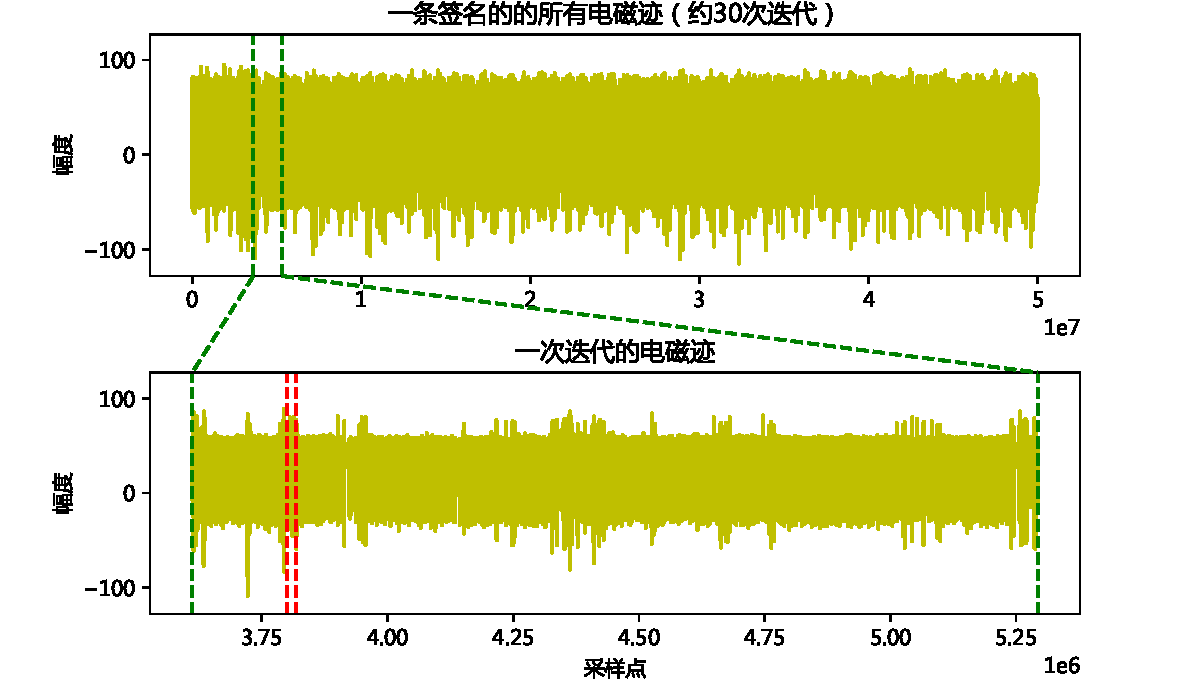
\includegraphics[width=\textwidth]{onetrs}
			\bicaption{\enspace ECDSA实现信息泄漏范围}{\enspace ECDSA implementation EM leakage range}
			\label{fig:onetrs}
		\end{center}
	\end{figure}
	
	%	在阶段一,我们首先对电磁迹分块(对于本文,第0至359个采样点的所对应的电磁迹的幅度构成第0个块,第360至719个采样点所对应的电磁迹的幅度构成第1个块,以此类推),每块的方差所构成的数列可以与电磁迹相对应,如\figureref{fig:halfphase1}的上、中两幅图所示。从图中可以看到,直观看来电磁迹中较粗的条带(如横坐标为400000附近的区域)所计算出的分块的方差也较大,较细的条带(如横坐标为392000附近的区域)所计算出的分块的方差也较小。这说明分块计算方差考虑到了电磁迹总体的变化趋势,这有助于进一步定位每次迭代的起止位置。
	%	
	%	在计算出每块的方差后,按照阈值执行模数转换和去抖动的操作,去抖动后的数列依然可以与电磁迹相对应,如\figureref{fig:halfphase1}的上、下两幅图所示。从图中可以看到,模数转换和去抖动后的数列所绘制的波形图依然体现了电磁迹总体变化的趋势,并且减小了后续分析的难度(从处理实数数列变为处理01数列)。但是此时的数列依然存在噪声,方波的数量对于每次迭代还是各不相同的,这使得如果仅以此作为辅助信息划分每一次迭代需要让程序频繁进行交叉验证,从而大幅增加时间消耗。
	%	
	%	\begin{figure}[!h]
	%		\begin{center}
	%			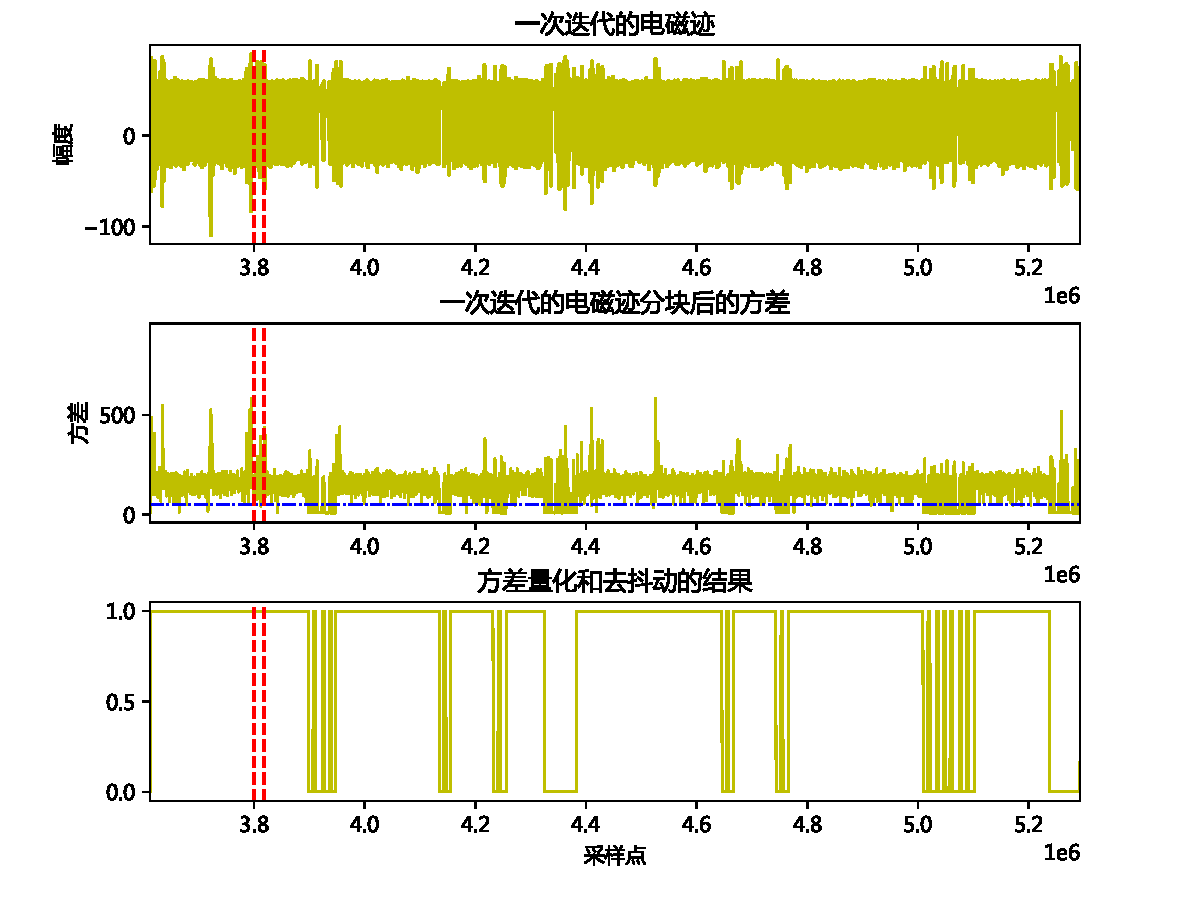
\includegraphics[width=\textwidth]{halfphase1}
	%			\bicaption{\enspace ECDSA实现电磁迹、电磁迹分块后的方差、方差模数转换和去抖动的结果}{\enspace ECDSA Implementation Raw Trace, the Variance of Trace Chunks and the Variance after Quantization and Anti-jitter}
	%			\label{fig:halfphase1}
	%		\end{center}
	%	\end{figure}
	%
	%	为了消除方差模数转换和去抖动的结果中的噪声,我们需要对它做进一步处理。使用模糊函数减小结果中的噪声以及降低层次细节,最终模糊后的数列依然可以与电磁迹相对应,如\figureref{fig:fullphase1}的上、中两幅图所示。从图中可以看到,相比于模糊前,模糊后的数列所绘制的波形图变化更为平缓,偶然的噪声也因为平均了邻域的数值而被减弱。
	%	
	%	在进行模糊后,数列又从01数列变为实数数列,增加了分析的难度。按照新的阈值重新执行模数转换和去抖动的操作,最终的数列还是可以与电磁迹相对应,如\figureref{fig:fullphase1}的上、下两幅图所示。从图中可以看到,模数转换和去抖动仅消除了被模糊所减弱的噪声,减小了后续分析的难度而没有产生其他负面影响。
	%
	随机选取部分计算结果,人工地对标注的POIs范围和在\poifanwei 之后计算出的辅助信息进行对比,如\figureref{fig:fullphase1}所示。\figureref{fig:fullphase1}中红色虚线代表人工标注的POIs范围,绿色虚线代表计算出的辅助信息。比较的内容是每次迭代中人工标注的POIs范围(最右边的红色虚线)与计算出的辅助信息(最左边的绿色虚线)横坐标值之差$\delta$。这些差值的标准差远小于均值,计算出的辅助信息与随机的横坐标有区别的显著水平达到99.999\%。\poifanwei 有效,可以达到与人工标注同样的效果。
	
	\begin{figure}[!h]
		\begin{center}
			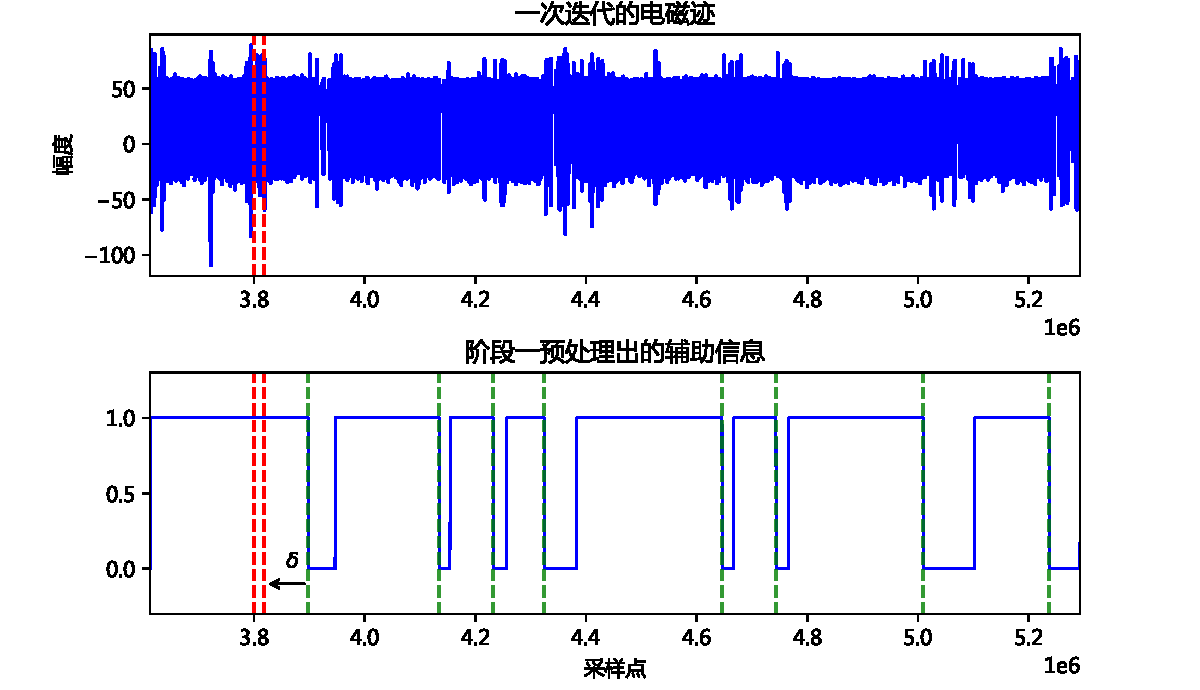
\includegraphics[width=\textwidth]{fullphase1}
			\bicaption{\enspace 计算出的关于电磁子迹的辅助信息}{\enspace Calculated auxiliary information on an EM subtrace}
			\label{fig:fullphase1}
		\end{center}
	\end{figure}
	
	\begin{figure}[!h]
		\begin{center}
			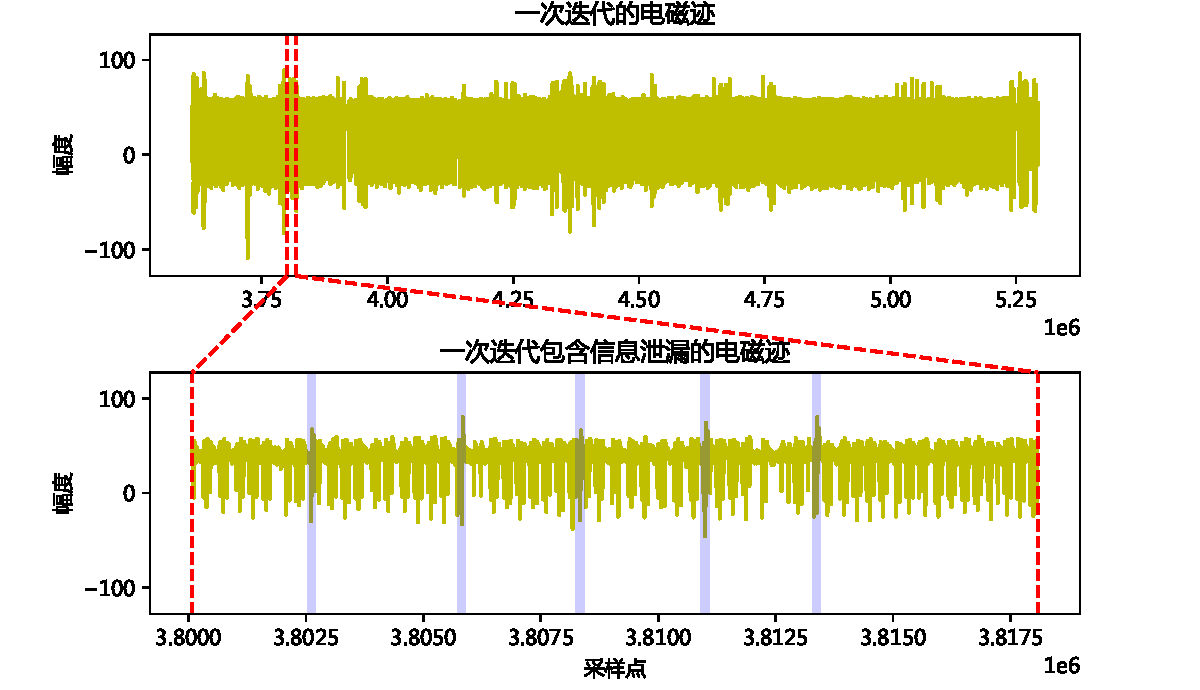
\includegraphics[width=\textwidth]{onetrsleak}
			\bicaption{\enspace 电磁子迹中特征点}{\enspace POIs in an EM subtrace}
			\label{fig:onetrsleak}
		\end{center}
	\end{figure}
	
	%到目前为止,我们可以准确划分出每次迭代,并找出其所对应的电磁迹的泄漏范围,但是还是不能准确确定泄漏位置。
	\figureref{fig:onetrsleak}绘制了所采集到的一条电磁迹在人工标注的泄漏范围内的波形图,其中五处浅蓝色条带是人工标注的POIs。我们期望在\yuchuli 之后可以类似地找到POIs。
{	
	%	使用简单的统计信息难以找到信息泄漏位置。为了解决这个问题,我们使用更复杂的数学工具分析采样点之间内在的联系。我们构造了一个模板,计算模板与所有模板所确定的采样点的邻域各自的协方差作为统计指标用于后续分析。\figureref{fig:rhovscov}展示了使用同一个模板所计算出的协方差与相关系数。从图中可以看到人工标注的信息泄漏位置与相关系数曲线的峰值恰好对应,但是难以和相关系数曲线峰值对应。例如,人工标注的第四处信息泄漏,在协方差曲线的对应位置有显著的峰值,但是在相关系数曲线中对应位置没有特征使得此位置可以从其他假阳性中区分出来。
	%	
	%	\begin{figure}[!h]
	%		\begin{center}
	%			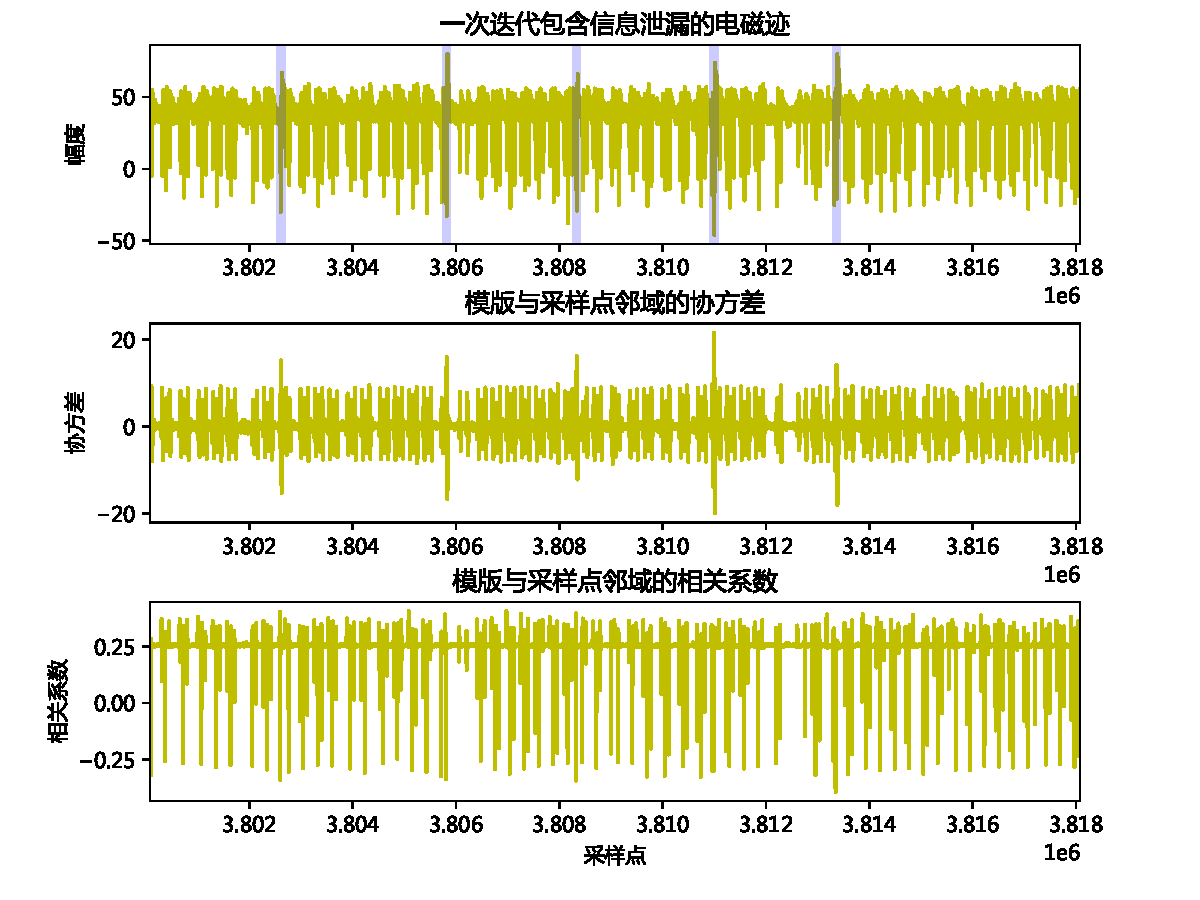
\includegraphics[width=\textwidth]{rhovscov}
	%			\bicaption{\enspace ECDSA实现信息泄漏及其对应的协方差与相关系数}{\enspace ECDSA Implementation EM Leakages and its Corresponding Covariance and Correlation Coefficient}
	%			\label{fig:rhovscov}
	%		\end{center}
	%	\end{figure}
	%
	%	\begin{figure}[!h]
	%		\begin{center}
	%			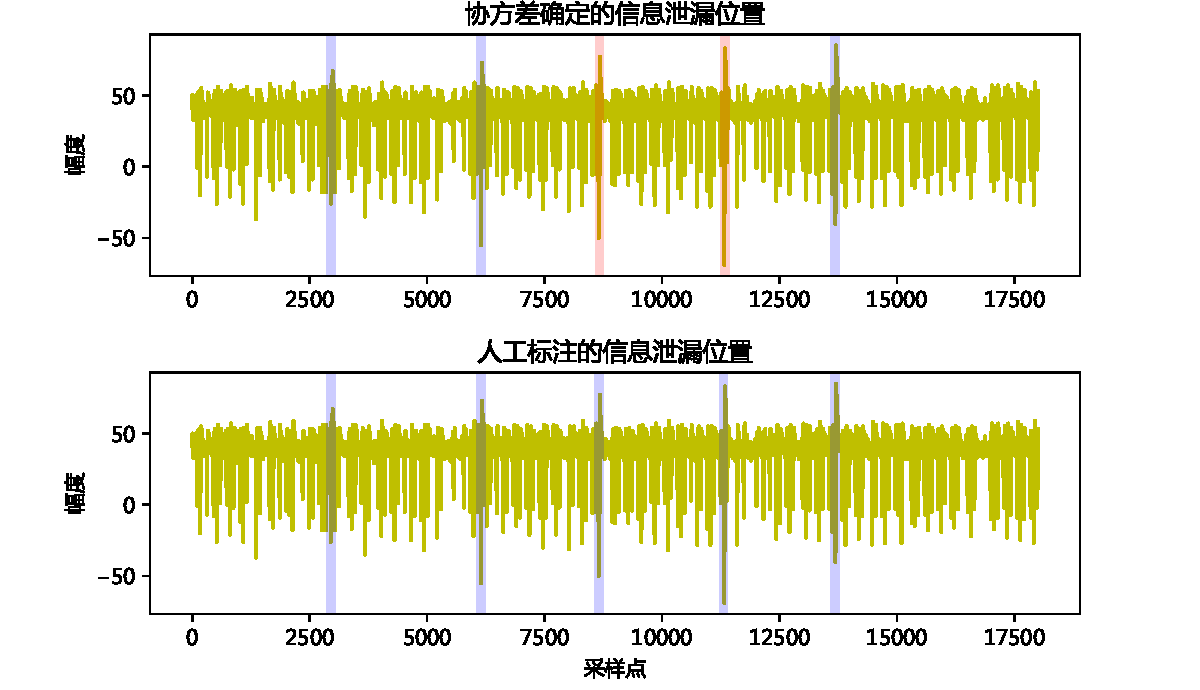
\includegraphics[width=\textwidth]{badmark}
	%			\bicaption{\enspace 计算出的错误信息泄漏位置和标注的信息泄漏位置的差异较小的情况}{\enspace Subtle Differences between Labeled and Wrongly Calculated Leak Positions}
	%			\label{fig:badmark}
	%		\end{center}
	%	\end{figure}
	%	
	%	尽管使用协方差已经帮助找到信息泄漏位置,但是我们在后续研究中发现以此确定的信息泄漏位置可能存在问题,如\figureref{fig:badmark}所示。从图中可以看到,协方差的前5个极值点所确定的信息泄漏位置中,红色条带标注位置是错误的,并不能对应到人工标注的泄漏位置。虽然图中看起来偏差不大,但对应的电磁迹片段和实际信息泄漏完全不符,这会导致后续恢复信息泄漏失败。出现偏差是因为取极值点操作不区分极大值点还是极小值点,从而引入一个系统误差。我们对这种系统误差进行人工统计,在取极值点之后判断是极大值点还是极小值点并据此进行校正,消除系统误差。
	%	
	%	除此之外,有一定信息泄漏存在变形的情况,这使得它对应的协方差并不是前5个极值,而是位于稍微靠后的位置,如第6大的极值(\figureref{fig:badmark2})。本文尝试后发现,对于所采集的电磁迹,每次迭代取前9个极值点,有超过95\%的概率能找到五个极值点,这五个极值点校正后与人工标注的泄漏位置的几乎重合。
	%	
	%	\begin{figure}[!h]
	%		\begin{center}
	%			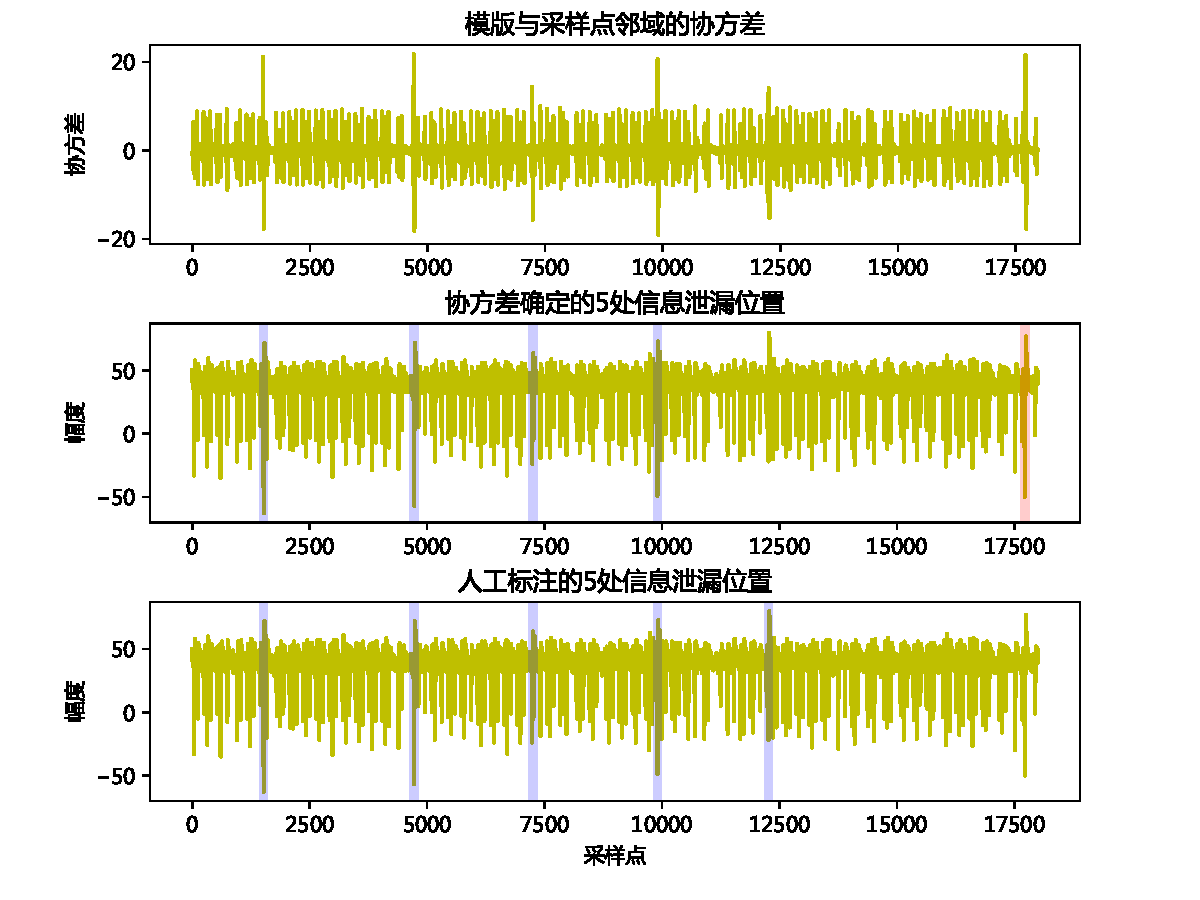
\includegraphics[width=\textwidth]{badmark2}
	%			\bicaption{\enspace 计算出的错误信息泄漏位置和标注的信息泄漏位置的差异较大的情况}{\enspace Substantial Differences between Labeled and Wrongly Calculated Leak Positions}
	%			\label{fig:badmark2}
	%		\end{center}
	%	\end{figure}
	%
	%	为了准确刻画这种重合程度,本文对信息泄漏位置之间采样点的距离建立模板,如\figureref{fig:lambda10}所示。对于一次迭代所对应的多处泄漏,我们认为信息泄漏之间采样点的距离$\delta_0,\delta_1,\dots,\delta_9$应当服从正态分布。\figureref{fig:delta-l0-r1detail}展示了$\delta_0$前1000个样本的概率直方图,从完整的直方图中可以知道,对于大部分迭代所对应的电磁迹,使用协方差找到的第0处信息泄漏位置和第1处信息泄漏位置相隔的采样点个数在3199左右,但是还存在极少数的情况会找错第0处泄漏位置或第1处泄漏位置,这对应于直方图在某些异常的位置(如2516)频数不为0。将数据比较集中的部分进行放大,我们进一步发现直方图可以大致分为三个区间:[3170,3191),[3191,3209)和[3209,3230)。对于区间[3191,3209),它是样本最集中的区域,频数直方图和竖直拉伸后的正态分布曲线(图中蓝色曲线)比较重合,这说明假设$\delta_0$服从正态分布是合理的。另外两个区间不是样本最集中的区域,但是频数直方图也和竖直拉伸后的正态分布曲线(图中黄色、程色曲线)比较重合。实际上,三个区间分别对应这样的情况:
	%	
	%	\begin{itemize}
	%		\item 如果第0处信息泄漏位置是通过协方差取极小值点得出,而第1处信息泄漏位置是通过协方差取极大值点得出,那么这向第0、1处信息泄漏之间采样点的距离中引入了一个小于0的系统误差,$\delta_0$的样本值很可能落在[3170,3191);
	%		\item 如果第0、1处信息泄漏位置通过协方差都取极大值点或都取极小值点得出,这没有向第0、1处信息泄漏之间采样点的距离引入系统误差,那么$\delta_0$的样本值很可能落在[3191,3209);
	%		\item 如果第0处信息泄漏位置是通过协方差取极大值点得出,而第1处信息泄漏位置是通过协方差取极小值点得出,那么这向第0、1处信息泄漏之间采样点的距离中引入了一个大于0的系统误差,$\delta_0$样本值很可能落在[3209,3230)。
	%	\end{itemize}
	%
	%	这进一步说明取极值点操作应当区分极大值点还是极小值点并及时校正,从而避免系统误差。校正之后,频数直方图数据分布变得更集中了。对于$\delta_1,\delta_2,\dots,\delta_9$,他们的情况和$\delta_0$类似,唯一不同之处在于正态分布的均值和方差一般是不同的,如\appfigureref{appfig:deltaall}所示,因此总共需要计算10次时间的模板。
	%	
	%	%视为我们人工对少量(10条电磁迹合计约300次迭代)电磁迹的信息泄漏位置进行标注,统计这些位置之间的差值的均值和方差,作为刻画重合程度的模板。
	%	
	%	\begin{figure}[!h]
	%		\begin{center}
	%			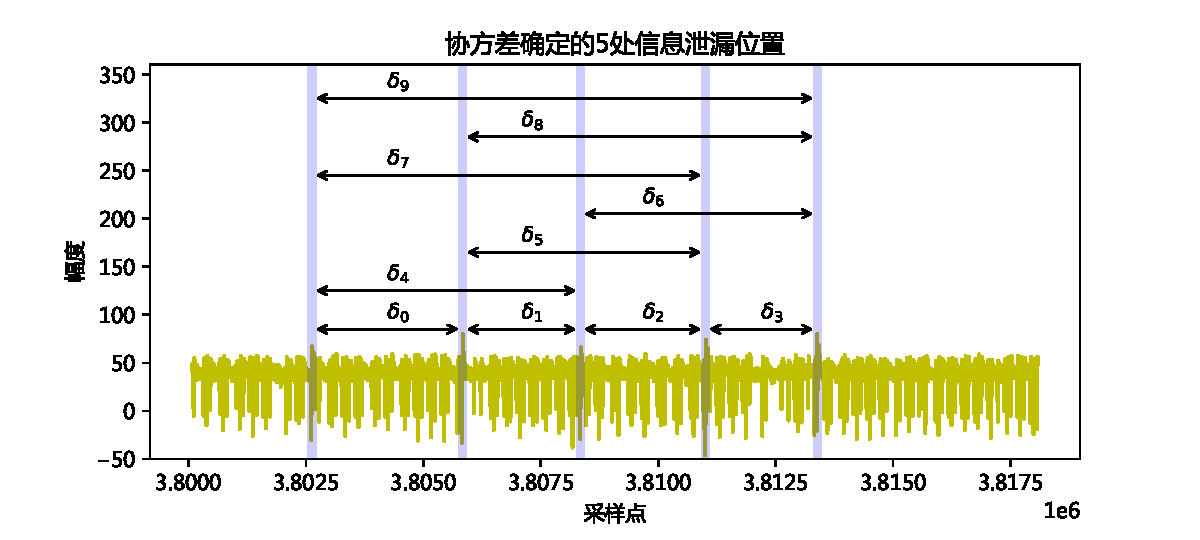
\includegraphics[width=\textwidth]{lambda10}
	%			\bicaption{\enspace 信息泄漏位置之间的距离示意图}{\enspace Demostration of Calculating Distance between Leak Positions}
	%			\label{fig:lambda10}
	%		\end{center}
	%	\end{figure}
	%	
	%	\begin{figure}[!h]
	%		\begin{center}
	%			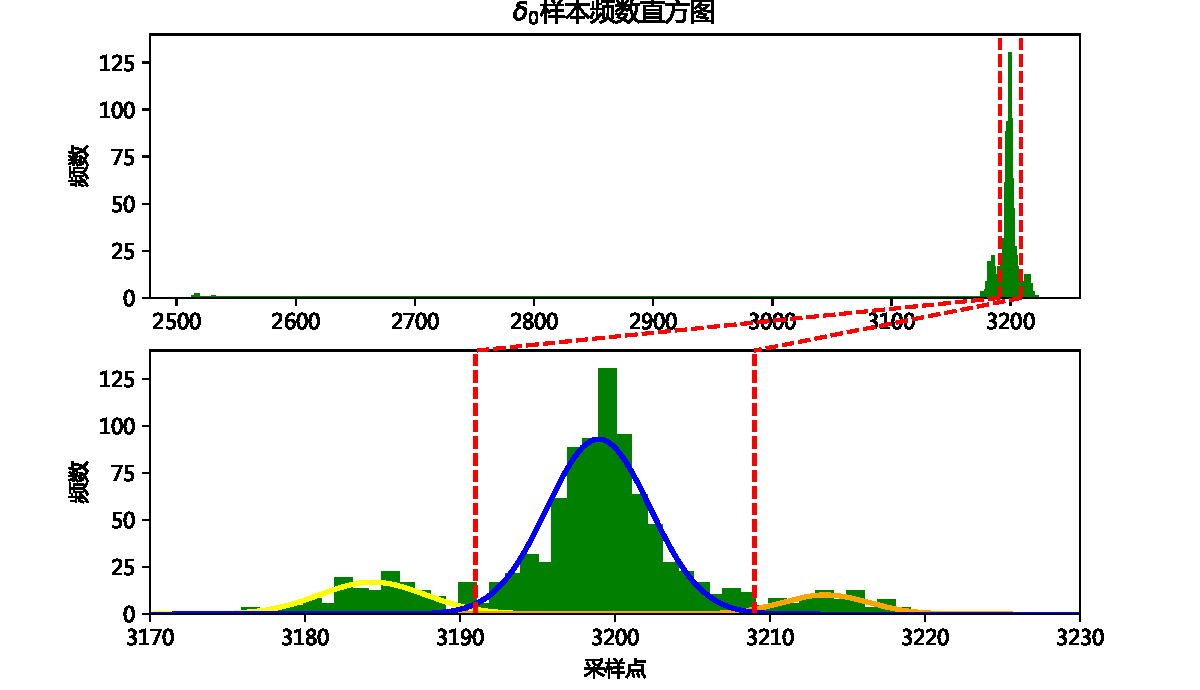
\includegraphics[width=\textwidth]{delta-l0-r1detail}
	%			\bicaption{\enspace 1000个$\delta_0$的样本频数直方图}{\enspace Frequency Histogram of 1000 $\delta_0$ Samples}
	%			\label{fig:delta-l0-r1detail}
	%		\end{center}
	%	\end{figure}
	%
	%	使用校正后的前9个极值点以及预计算的模板,\algorithmref{alg:checkdelta}可以筛选出符合模板的极值点,进而确定信息泄漏位置,如\figureref{fig:select9}所示。虽然前9个极值点中一定会有错误的,但是进行模板检查之后可以排除这种错误,从而准确选出理论上会对应信息泄漏的5个极值点。在极少的情况下(占所有情况的比例少于5\%),找不到符合模板的极值点,因此无法确定某一次迭代的信息泄漏位置,也就无法恢复此次迭代的信息泄漏。需要注意的是,这种情况不会直接导致攻击失败,只是会增加找到可利用(连续4比特)的敏感信息泄漏的难度。
	%	
	%	\begin{figure}[!h]
	%		\begin{center}
	%			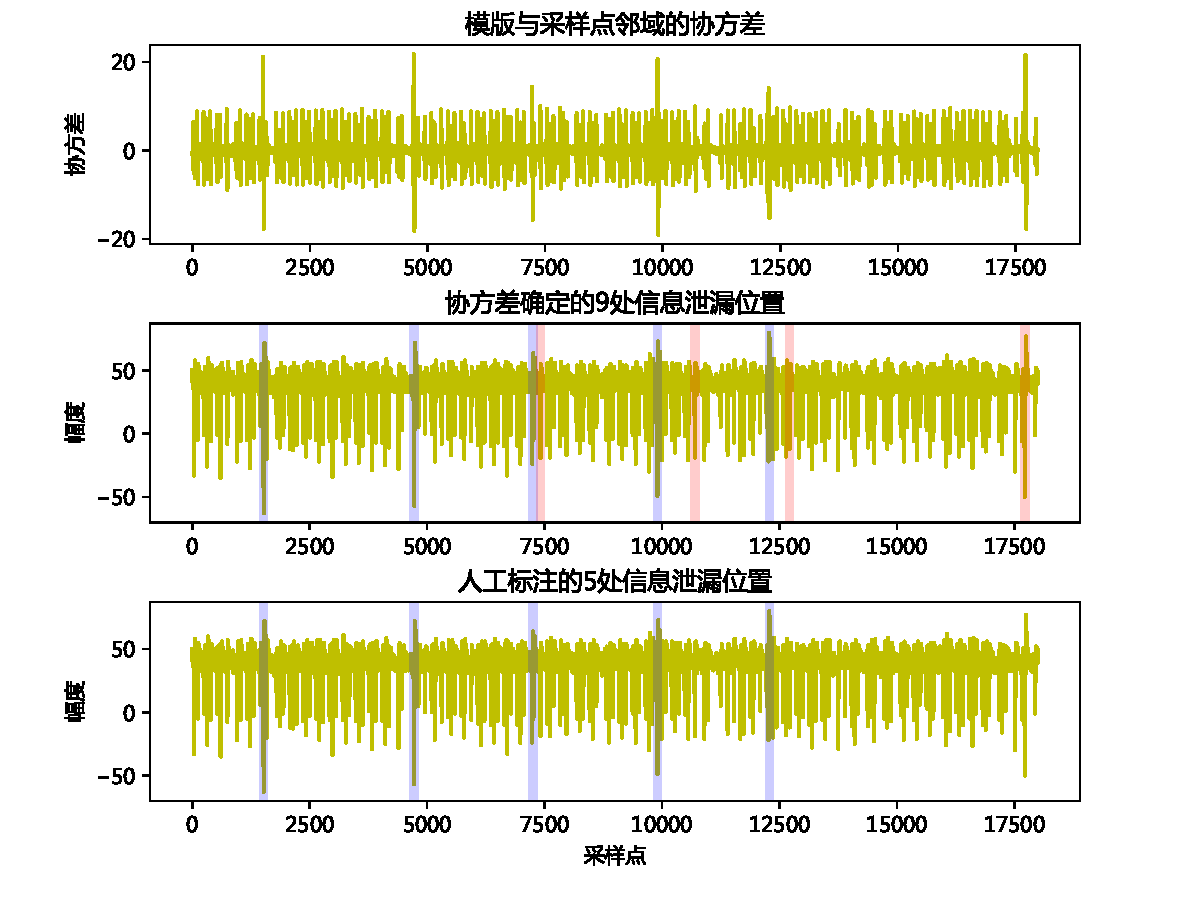
\includegraphics[width=\textwidth]{select9}
	%			\bicaption{\enspace 协方差极值点不能确定的信息泄漏位置的情况}{\enspace Failing to Determine the Leak Position using Argmax of Covariance}
	%			\label{fig:select9}
	%		\end{center}
	%	\end{figure}
}

	随机选取部分计算结果,人工地对标注的POIs和在\yuchuli 之后计算出的POIs进行对比。对比的方法是,根据POIs对电磁子迹进行对齐,量化评价电磁子迹的对齐程度可以从侧面反映POIs提取的准确程度。
	获得了POIs后,我们从相应位置及其邻域\footnote{邻域的大小可以自行设定。在本文中,邻域设定为以当前位置为中心,左右各150个采样点的区间。}提取电磁子迹并重新对采样点编号。\figureref{fig:aligndemo}绘制了提取出的每次迭代的第二处包含信息泄漏的电磁子迹,上图是500条中间值$\tilde\nonce_j=1$的电磁子迹以及500条中间值$\tilde\nonce_j=3$的电磁子迹,下图是这1000条电磁子迹进行TVLA的结果。下图TVLA结果在第140个采样点取得极值且超过阈值4.5,因此提取出的电磁子迹在第140个采样点处对齐且存在敏感中间值泄漏的置信水平达到99.999\%。上图中曲线的颜色的深浅可以体现某一类电磁子迹的集中程度,可以看出,$\tilde\nonce_j=1$所对应的电磁子迹在第140个采样点的幅度总体来说是比$\tilde\nonce_j=3$所对应的幅度大,这与TVLA的结果是一致的。根据结果认为\yuchuli 达到了预期效果,可以准确确定POIs,也能在此基础上进行电磁子迹的对齐。
	
	\begin{figure}[!h]
		\begin{center}
			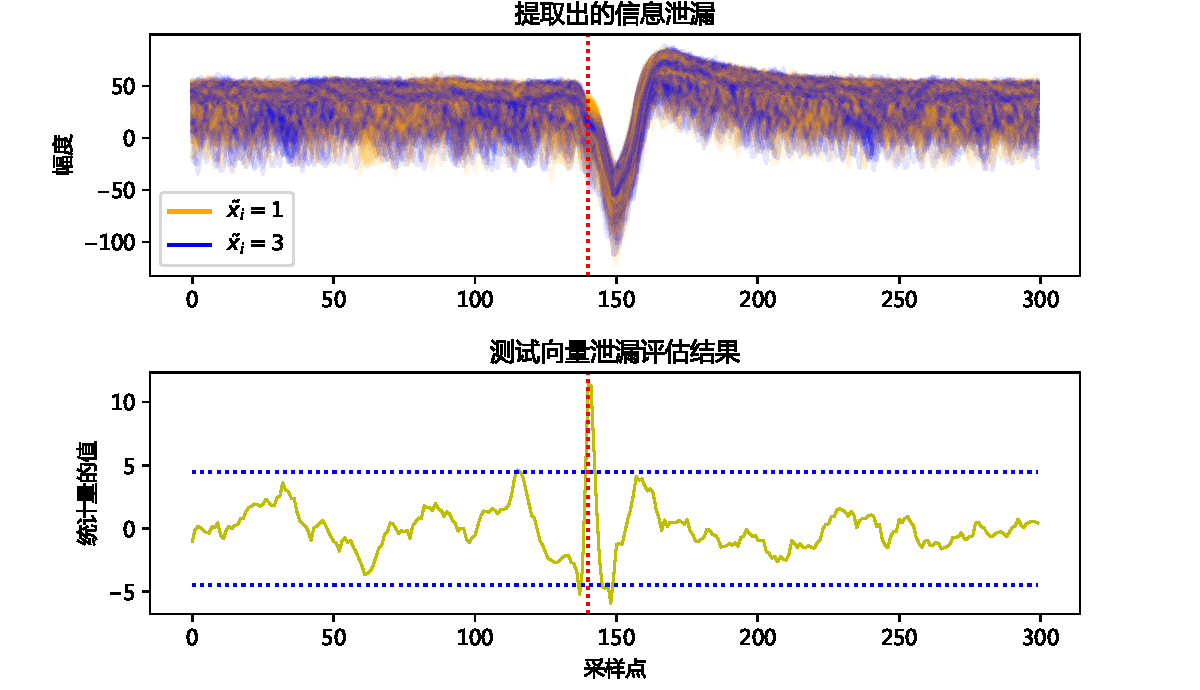
\includegraphics[width=\textwidth]{aligndemo}
			\bicaption{\enspace 每次迭代包含第二处信息泄漏的电磁子迹及其TVLA结果}{\enspace Subtraces containing the second leakage and their TVLA result}
			\label{fig:aligndemo}
		\end{center}
	\end{figure}

	对于每次迭代包含敏感信息泄漏的电磁迹,不同中间值$\tilde\nonce_i$之间TVLA结果见\appfigureref{appfig:aligndemoall}。
	
	\begin{figure}[!h]
		\centering
		\begin{subfigure}[b]{\trif\textwidth}
			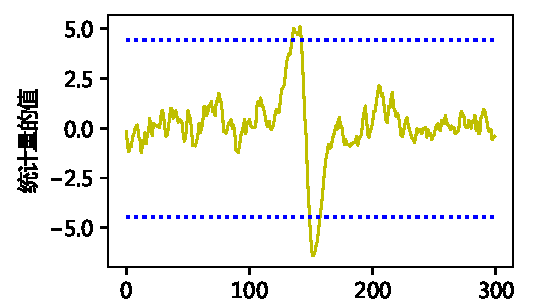
\includegraphics[width=\textwidth]{appfig/aligndemo-i0-j1-k2}
			\caption{第一处POIs,$\tilde\nonce_j=1$ vs $\tilde\nonce_j=2$}
			\label{fig:aligndemo012}
		\end{subfigure}%
		~% add desired spacing
		\begin{subfigure}[b]{\trif\textwidth}
			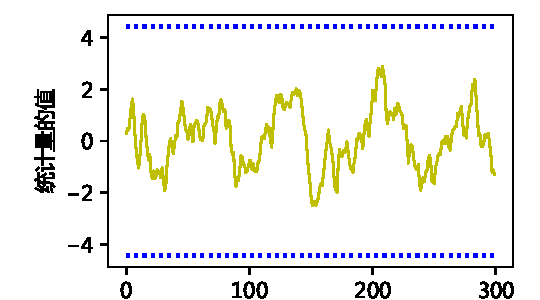
\includegraphics[width=\textwidth]{appfig/aligndemo-i0-j1-k3}
			\caption{第一处POIs,$\tilde\nonce_j=1$ vs $\tilde\nonce_j=3$}
			\label{fig:aligndemo013}
		\end{subfigure}
		~% add desired spacing
		\begin{subfigure}[b]{\trif\textwidth}
			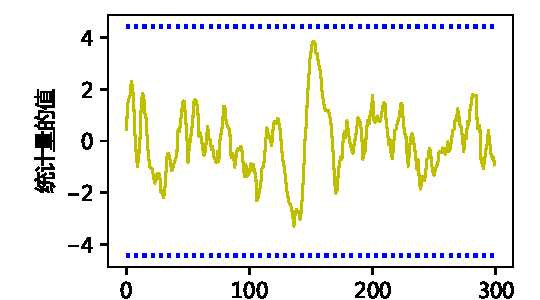
\includegraphics[width=\textwidth]{appfig/aligndemo-i0-j2-k3}
			\caption{第一处POIs,$\tilde\nonce_j=2$ vs $\tilde\nonce_j=3$}
			\label{fig:aligndemo023}
		\end{subfigure}
		\\% line break
		\begin{subfigure}[b]{\trif\textwidth}
			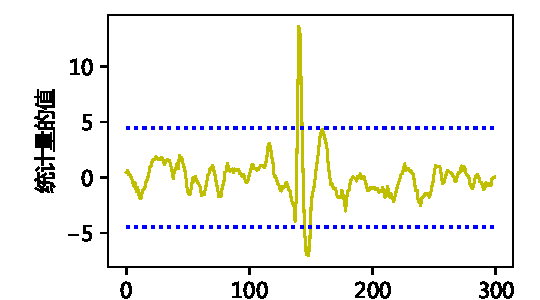
\includegraphics[width=\textwidth]{appfig/aligndemo-i1-j1-k2}
			\caption{第二处POIs,$\tilde\nonce_j=1$ vs $\tilde\nonce_j=2$}
			\label{fig:aligndemo112}
		\end{subfigure}%
		~% add desired spacing
		\begin{subfigure}[b]{\trif\textwidth}
			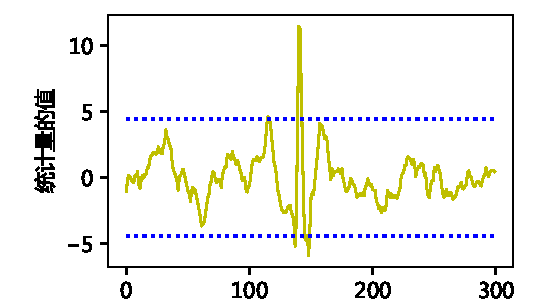
\includegraphics[width=\textwidth]{appfig/aligndemo-i1-j1-k3}
			\caption{第二处POIs,$\tilde\nonce_j=1$ vs $\tilde\nonce_j=3$}
			\label{fig:aligndemo113}
		\end{subfigure}
		~% add desired spacing
		\begin{subfigure}[b]{\trif\textwidth}
			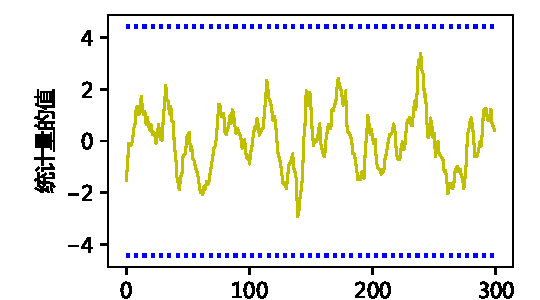
\includegraphics[width=\textwidth]{appfig/aligndemo-i1-j2-k3}
			\caption{第二处POIs,$\tilde\nonce_j=2$ vs $\tilde\nonce_j=3$}
			\label{fig:aligndemo123}
		\end{subfigure}
		\\% line break
		\begin{subfigure}[b]{\trif\textwidth}
			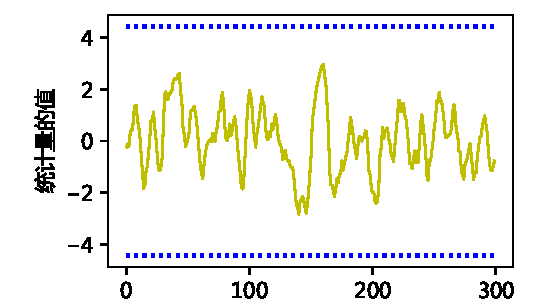
\includegraphics[width=\textwidth]{appfig/aligndemo-i2-j1-k2}
			\caption{第三处POIs,$\tilde\nonce_j=1$ vs $\tilde\nonce_j=2$}
			\label{fig:aligndemo212}
		\end{subfigure}%
		~% add desired spacing
		\begin{subfigure}[b]{\trif\textwidth}
			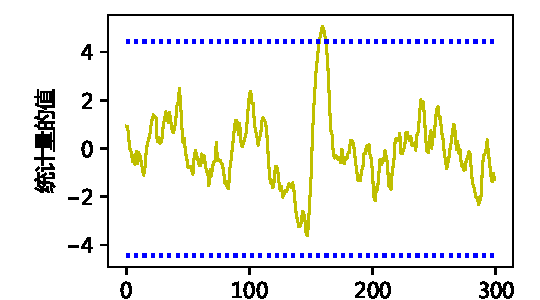
\includegraphics[width=\textwidth]{appfig/aligndemo-i2-j1-k3}
			\caption{第三处POIs,$\tilde\nonce_j=1$ vs $\tilde\nonce_j=3$}
			\label{fig:aligndemo213}
		\end{subfigure}
		~% add desired spacing
		\begin{subfigure}[b]{\trif\textwidth}
			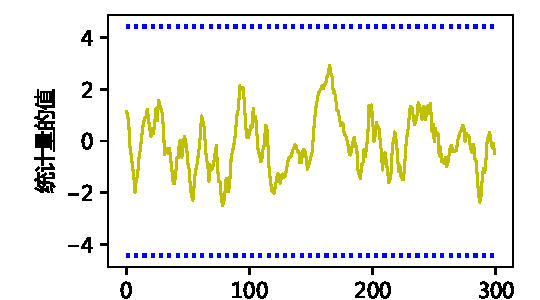
\includegraphics[width=\textwidth]{appfig/aligndemo-i2-j2-k3}
			\caption{第三处POIs,$\tilde\nonce_j=2$ vs $\tilde\nonce_j=3$}
			\label{fig:aligndemo223}
		\end{subfigure}
		\\% line break
		\begin{subfigure}[b]{\trif\textwidth}
			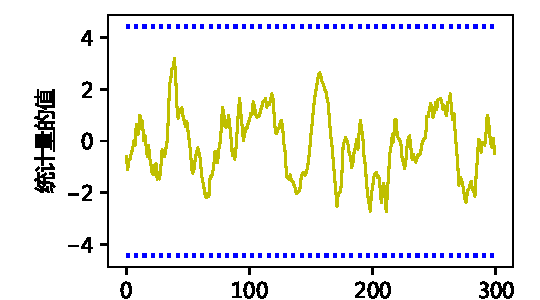
\includegraphics[width=\textwidth]{appfig/aligndemo-i3-j1-k2}
			\caption{第四处POIs,$\tilde\nonce_j=1$ vs $\tilde\nonce_j=2$}
			\label{fig:aligndemo312}
		\end{subfigure}%
		~% add desired spacing
		\begin{subfigure}[b]{\trif\textwidth}
			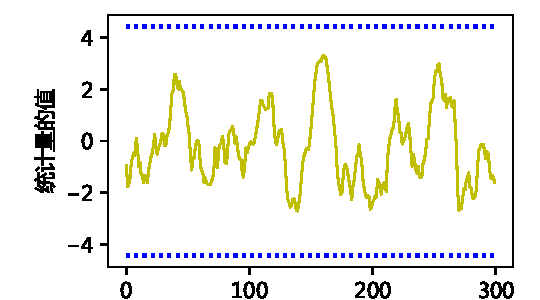
\includegraphics[width=\textwidth]{appfig/aligndemo-i3-j1-k3}
			\caption{第四处POIs,$\tilde\nonce_j=1$ vs $\tilde\nonce_j=3$}
			\label{fig:aligndemo313}
		\end{subfigure}
		~% add desired spacing
		\begin{subfigure}[b]{\trif\textwidth}
			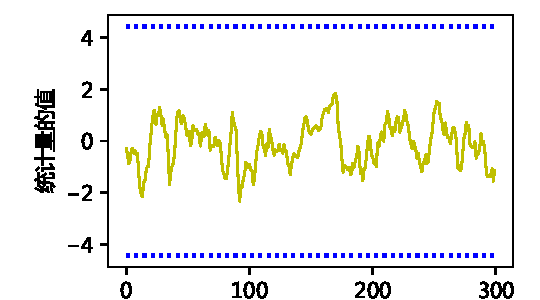
\includegraphics[width=\textwidth]{appfig/aligndemo-i3-j2-k3}
			\caption{第四处POIs,$\tilde\nonce_j=2$ vs $\tilde\nonce_j=3$}
			\label{fig:aligndemo323}
		\end{subfigure}
		\\% line break
		\bicaption{\enspace 合计1000次迭代所对应的电磁迹TVLA结果}{\enspace TLVA results of 1000 subtraces}
		\label{appfig:aligndemoall}
	\end{figure}

{	
	%	在评估阶段,我们只能知道每个$\tilde \nonce_i$的值但是不能准确知道每个$\leakedmultiplier_i$的值,如\tableref{tab:partialknownti}所示。我们从所有迭代含有信息泄漏的电磁迹中过滤出了对应的$\leakedmultiplier_i$完全确定的电磁迹(即从所有电磁迹中只选出对应的$\tilde \nonce_i\neq0$的电磁迹)并使用TVLA进行泄漏检测。对于每次迭代包含其它信息泄漏的电磁迹,不同中间值$\leakedmultiplier_i$之间TVLA结果见\appfigureref{appfig:aligndemoall}。
	%	
	%	\begin{table}[!htb]
	%		\bicaption{\enspace 评估时可以推断的$\leakedmultiplier_i$的信息}{\enspace Deduced $\leakedmultiplier_i$ for Evaluation}
	%		\label{tab:partialknownti}
	%		\centering
	%		\begin{subtable}{\twof\textwidth}
	%			\centering
	%			\begin{tabular}{cc|ccc}
	%				\hline
	%				\multicolumn{2}{c|}{\multirow{2}{*}{$\Pr[\leakedmultiplier_i=v|\tilde \nonce_i=w]$}} & \multicolumn{3}{c}{$v$} \\
	%				%\cline{3-5}
	%				\multicolumn{2}{c|}{}& 1 & 2 & 3 \\
	%				\hline
	%				\multirow{4}{*}{$w$} & 0 & $\frac12$ & $\frac14$ & $\frac14$ \\
	%				%\cline{2-5}
	%				& 1 & 1 & 0 & 0 \\
	%				%\cline{2-5}
	%				& 2 & 0 & 1 & 0 \\
	%				%\cline{2-5}
	%				& 3 & 0 & 0 & 1 \\
	%				\hline
	%			\end{tabular}
	%			\subcaption{$\leakedmultiplier_i$的条件分布列}
	%			\label{tab:partialknowntidetail}
	%		\end{subtable}\hfill
	%		\begin{subtable}{\twof\textwidth}
	%			\centering
	%			\begin{tabular}{c|cc}
	%				\hline
	%				$\tilde \nonce_i$数值&能否知道$\leakedmultiplier_i$数值&$\leakedmultiplier_i$数值\\
	%				\hline
	%				0 & 否 & /\\
	%				1 & 是 & 1\\
	%				2 & 是 & 2\\
	%				3 & 是 & 3\\
	%				\hline
	%			\end{tabular}
	%			\subcaption{由$\tilde \nonce_i$可以推断的$\leakedmultiplier_i$的信息}
	%			\label{tab:partialknownticonclusion}
	%		\end{subtable}
	%	\end{table}
	%
	%	总的来说,进行阶段二之后我们可以成功提取包含信息泄漏的电磁迹且能通过TVLA检测出存在信息泄漏。经过阶段一和阶段二,提取出包含信息泄漏的电磁迹后,还需要从中恢复信息泄漏才能完成对智能卡ECDSA实现的侧信道分析整个流程。
}

	\subsection{未采用数据增强的模板构建结果}
	\algorithmref{alg:filter}会输出五个数据集,使用任何一个可以获得的效果是类似的。实验发现在仅使用一组电磁子迹的情况下使用$L_1^{out}$可以获得最优的结果,因此后续只列举利用$L_1^{out}$和$Label^{out}$进行建模和攻击的结果。提取POIs并构造数据集后,将$cnt\approx100000$个样本拆分为5组,每组20000个样本(舍去剩余的)。这么做的原因是可以对于同一张双界面商用智能卡所采集的电磁迹,构造出的数据集可以进行互相独立的五次实验。每一组又拆分为训练集、验证集和测试集,大小分别设置为10000、5000、5000。本文中训练集设置相比于通常训练集的占比80\%较少有两个原因,一个是训练深度学习模型的数据增强后的训练集而数据增强后的训练集会比数据增强前更大,另一个原因是这样可以使得通用数据增强方法对DL-SCA提升的效果更明显。
	
	深度学习模型的超参数与\subsref{subs:useagmt}中深度学习模型设置一致。
	
	一组样本只进行一次实验,5组样本总共进行5组实验,最后的结果取5组中的最优。取最优的原因有两个,一个是在现实场景中攻击只用成功一次就说明攻击目标存在漏洞,另一个在大部分情况下是恢复私钥的时间只能在理论上进行估计而不能实际计算。
	
	在未采用数据增强方法时,DL-SCA使用$L_1^{out}$进行训练和验证的结果如\figureref{fig:ecdsanoda}所示。从图中可以看出随着训练轮次逐渐增加,验证集精确率逐渐提升,说明训练有效。在五次实验中,在训练完成后样本数量为5000的测试集中平均有1720.4个敏感中间值估计值为0,其准确率为91.35\%;有3279.6个敏感中间值估计值为1,其准确率为96.08\%。%精确率(使用极大似然估计时的\zyx ,见\subsref{subs:useagmt}中\textbf{攻击评估单元设置}部分。)可以达到91.35\%。%,在这种情况下,运用格方法恢复双界面商用智能卡ECDSA私钥的时间在理论上会超过七百万年。
	
	在特征点提取之后,电磁迹的采样点个数从5000万减小为300\footnote{$150*2=300$它表示邻域设定为以一个特征点为中心,左右各150个采样点的区间。},深度学习模型的所占用的存储空间变为原来的$3/500000$。数据处理前深度学习训练阶段会使用333条电磁迹训练20个训练轮次,计算量为$8.7\cdot10^{16}$浮点运算次数(Floating Point Operation,FLOP)。提取特征点构造新的数据集后深度学习训练阶段会使用一万条电磁子迹(333条电磁迹包含共9990次迭代的敏感中间值,这对应于9990条电磁子迹)训练20个训练轮次,计算量减少为$1.6\cdot10^{13}$FLOPs。对本文的实验环境而言,算力不超过3.2G\footnote{实际上CPU主频为3.2GHz,算力难以直接测量。在不考虑数据并行的情况下,CPU每个时钟周期执行最多一次浮点运算,此时算力数值大小不超过CPU主频数值大小。}每秒浮点运算次数,因此深度学习训练阶段所消耗的时间会从315天减小为8分钟。实际实验中,DL-SCA时间为490秒(8分10秒),与理论分析一致。%样本数量变为原来的30倍,因此深度学习模型训练阶段计算量减小为原来的$\frac{9}{50000}$。
	
	\begin{figure}[!h]
		\centering
		\begin{subfigure}[b]{\twof\textwidth}
			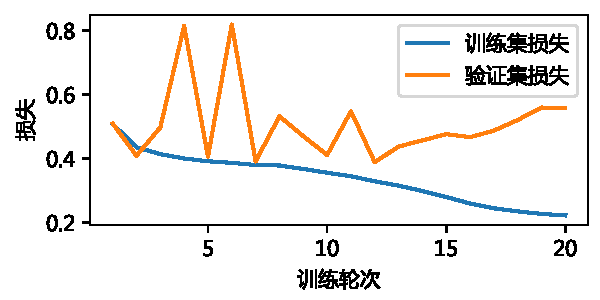
\includegraphics[width=\textwidth]{ecdsanodaloss}
			\caption{负对数交叉熵损失}
			\label{fig:ecdsanodaloss}
		\end{subfigure}%
		~% add desired spacing
		\begin{subfigure}[b]{\twof\textwidth}
			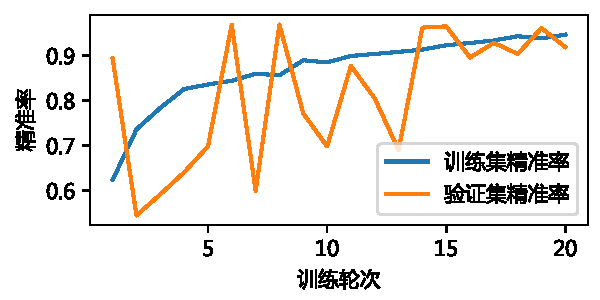
\includegraphics[width=\textwidth]{ecdsanodaprecision}
			\caption{精确率}
			\label{fig:ecdsanodaprecision}
		\end{subfigure}
		\\
		\bicaption{\enspace 无数据增强的DL-SCA训练和验证结果}{\enspace Training and validation results of DL-SCA without DA}
		\label{fig:ecdsanoda}
	\end{figure}

	\subsection{\shujuzengqiang 结果}
	
	采用面向基于深度学习侧信道分析的数据增强方法后,DL-SCA使用$L_1^{out}$进行训练和验证的结果如\figureref{fig:ecdsaada}所示。%在训练完成后,测试集精确率(使用极大似然估计时的\zyx )可以达到95.50\%。%,在这种情况下,运用格方法恢复双界面商用智能卡ECDSA私钥的时间在理论上会达到12.5年。
	在五次实验中,在训练完成后样本数量为5000的测试集中平均有1713.2个敏感中间值估计值为0,其准确率为95.50\%;有3286.8个敏感中间值估计值为1,其准确率为98.06\%。
	采用数据增强方法会导致DL-SCA时间由8分钟增长到1小时,还额外引入2分钟的数据增强时间,但是对于格方法减少的时间而言,所增加的时间可以忽略不计。
	
	\begin{figure}[!h]
		\centering
		\begin{subfigure}[b]{\twof\textwidth}
			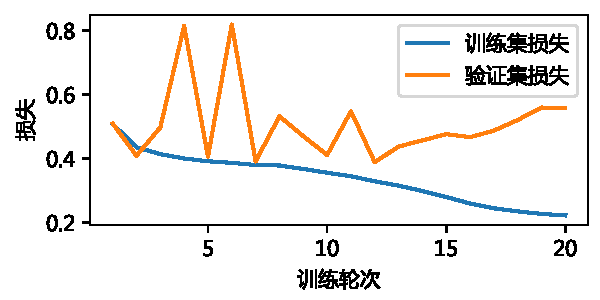
\includegraphics[width=\textwidth]{ecdsanodaloss}
			\caption{负对数交叉熵损失}
			\label{fig:ecdsaadaloss}
		\end{subfigure}%
		~% add desired spacing
		\begin{subfigure}[b]{\twof\textwidth}
			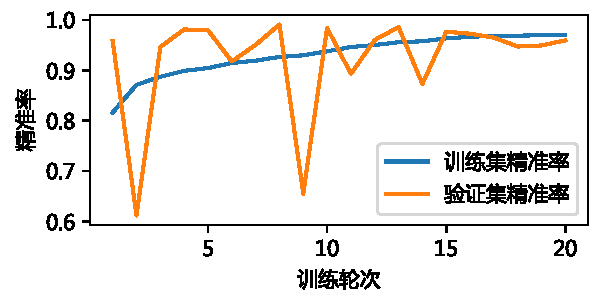
\includegraphics[width=\textwidth]{ecdsaadaprecision}
			\caption{精确率}
			\label{fig:ecdsaadaprecision}
		\end{subfigure}
		\\
		\bicaption{\enspace 采用通用数据增强方法的DL-SCA训练和验证结果}{\enspace Training and validation results of DL-SCA with general DA method}
		\label{fig:ecdsaada}
	\end{figure}

	\subsection{\jiashejianyanguji 结果}
	采用\jiashejianyanguji 方案后,DL-SCA使用$L_1^{out}$进行训练和验证的结果如\figureref{fig:ecdsatpr}所示。可以看出,无论是否采用数据增强方法,提高显著水平$\alpha$可以提高\zyx 。%在训练完成后,在显著水平$\alpha=0.51056$、使用本文采集的数据、独立进行5次进行深度学习模型的训练和测试、每次使用5000条电磁子迹进行测试的情况下,测试集\zyx 都达到100\%。%在这种情况下,理论上运用格方法可以恢复双界面商用智能卡ECDSA私钥,平均时间为400秒。
	在五次实验中,在训练完成后样本数量为5000的测试集中平均有981个敏感中间值估计值为0,其准确率为100\%;有4019个敏感中间值估计值为1,其准确率为75.89\%。

	通过与\shujuzengqiang 结果比较可以看出,\jiashejianyanguji 通过提高显著水平$\alpha$,提高\zyx。\jiashejianyanguji 会导致恢复nonce比特0的比例减小,恢复nonce比特1的准确率也减小。
	
	\begin{figure}[!h]
		\centering
		\begin{subfigure}[b]{\twof\textwidth}
			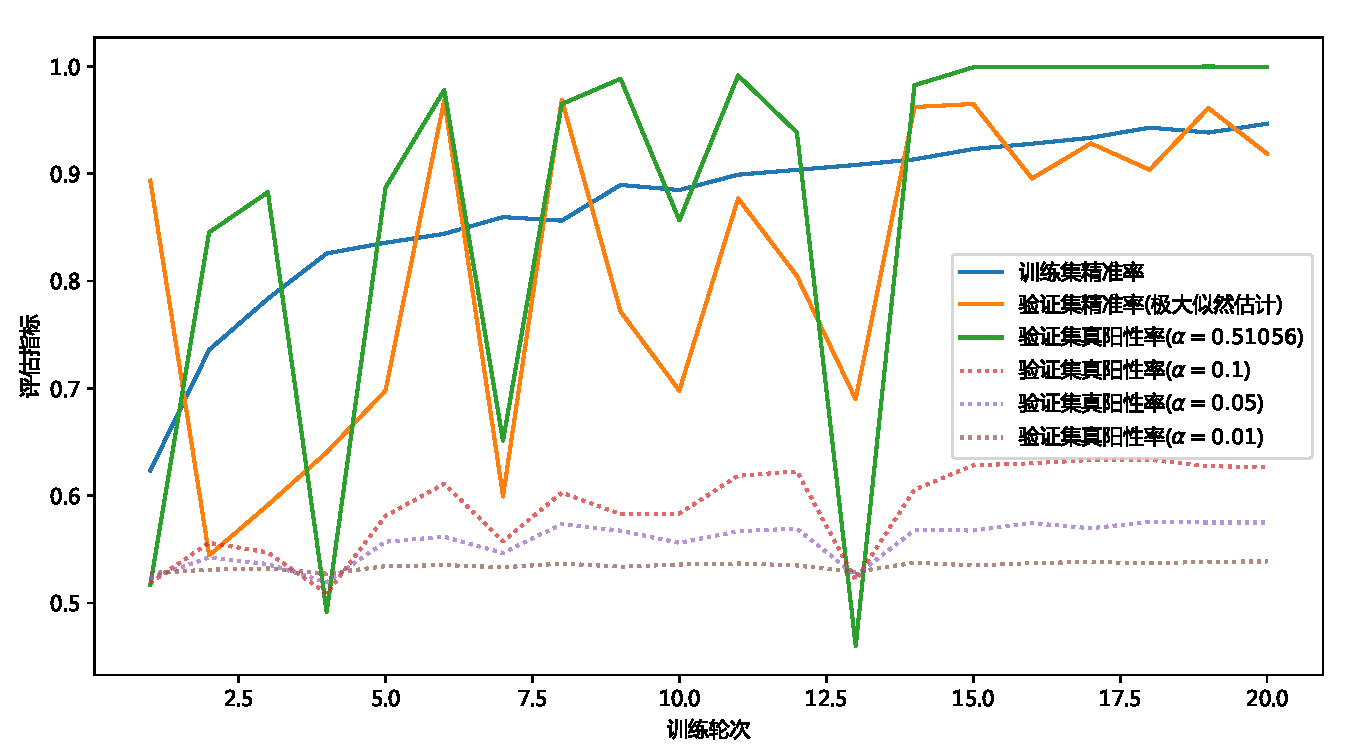
\includegraphics[width=\textwidth]{ecdsanodatpr}
			\caption{未采用数据增强}
			\label{fig:ecdsanodatpr}
		\end{subfigure}%
		~% add desired spacing
		\begin{subfigure}[b]{\twof\textwidth}
			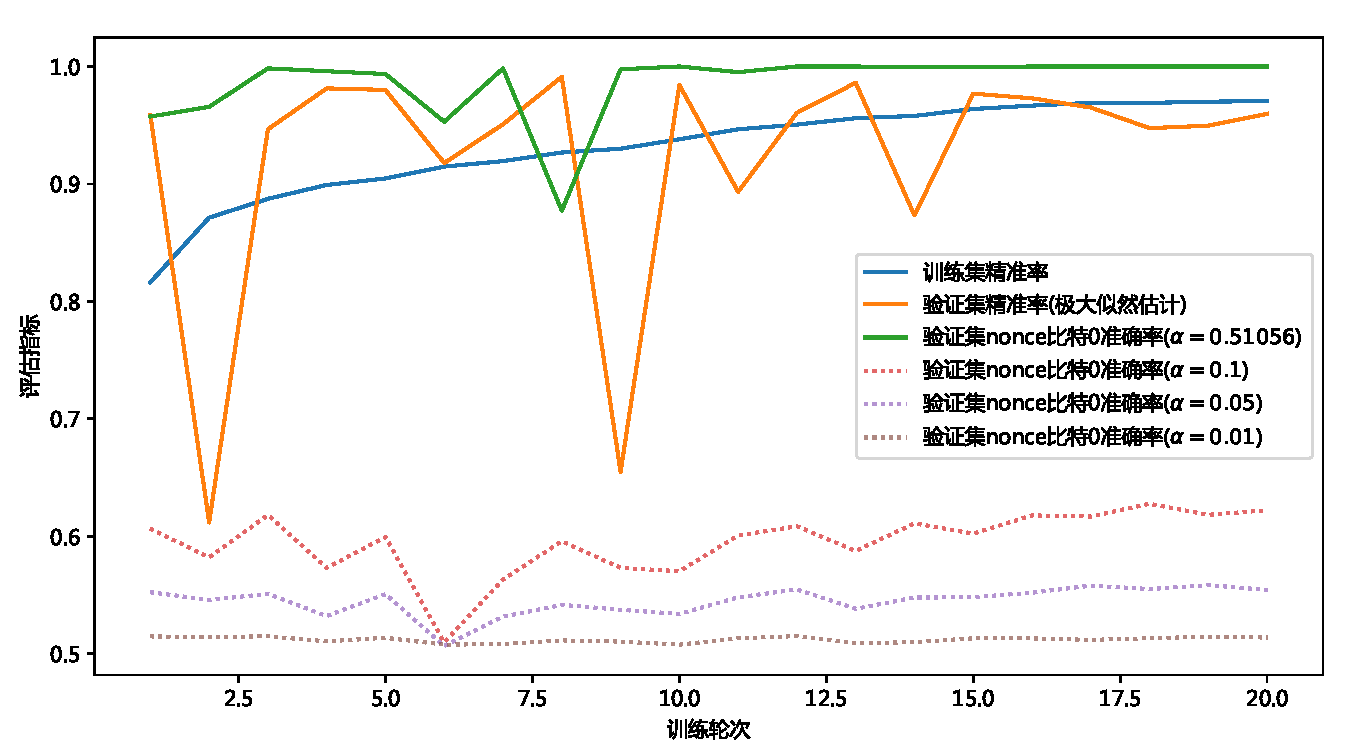
\includegraphics[width=\textwidth]{ecdsaadatpr}
			\caption{采用数据增强}
			\label{fig:ecdsaadatpr}
		\end{subfigure}
		\\
		\bicaption{\enspace DL-SCA训练和验证结果}{\enspace Training and validation results of DL-SCA}
		\label{fig:ecdsatpr}
	\end{figure}
	
	
	\subsection{电磁分析方法与格方法结合后效果}
	{\color{\xchange}
	
	\tableref{tab:improve}列举了本方法在型号为J3D081的Java卡进行电磁分析验证以及Roche等\citep{Roche21}在谷歌安全产品\textit{Google Titan Security Key}\citep{Titan}进行攻击的结果。两个研究对象使用了相同的安全微控制器芯片SmartMX\citep{p5x}。%暴力破解是逐一枚举$Z_q$中所有元素并逐一进行验证的方法,它描述了攻击密码算法时的最坏情况。Zaid等\citep{Zaid20}针对ASCADf(N=50)数据集设计的深度神经网络,调整网络输入为50000000,训练轮次为20之后理论上讲可以进行电磁分析攻击。
	Roche等\citep{Roche21}他们运用了滤波的预处理技术、聚类以及格方法实施攻击。本文运用了\yuchuli 预处理技术、面向基于深度学习侧信道分析的通用数据增强方法、\jiashejianyanguji 方案以及格方法实施攻击。
	
	\begin{table}[!h]
		\bicaption{\enspace 攻击相似芯片上ECDSA实现的技术效果}{\enspace Result of works that attack ECDSA implementation on similar chips}
		\label{tab:improve}
		\centering
		\small% fontsize
		%\setlength{\tabcolsep}{4pt}% column separation
		%\renewcommand{\arraystretch}{1.2}%row space 
		\begin{tabular}{ccc}
			\hline
			技术指标&Roche等\citep{Roche21}&本文\\
			\hline
			采集时间&6小时&1天\\
			预处理时间&/&3天\\
			数据增强时间&0&2分钟\\
			DL-SCA时间&0&1小时\\
			聚类时间&/&0\\
			\zyx&99.6\%&100\%\\
			\hline
		\end{tabular}
		\tabnote{数据不详使用斜杠/ 标记。}
	\end{table}

	%从可计算性的角度来看,枚举空间$q\approx2^{256}$(椭圆曲线$E$的阶)是个有限的数,使用暴力破解足以恢复ECDSA私钥。就本文的实验环境(处理器型号为Intel(R) Xeon(R) CPU E5-2667 v4 @ 3.20GHz,内存大小252GB)而言,枚举100000个元素并逐一验证需要约7秒。因此枚举$q$个元素进行暴力破解最坏需要$2.6\times10^{65}$年,平均需要$1.3\times10^{65}$年,这在现实中是难以接受的。暴力破解没有改进的空间,因此实际需要使用其他攻击思路,例如尝试使用侧信道分析恢复私钥。
	
	%将Zaid等\citep{Zaid20}的深度学习网络套用到侧信道分析的现实场景,理论可行但是实际存在时间开销长的问题。这也导致就本文的实验环境,无法计算准确的\zyx ,从而无法估计使用格方法所需要的时间。
	
	Roche等\citep{Roche21}等与本文的主要不同之处在于他们使用聚类的方法恢复敏感中间值,\zyx 可达到99.6\%。恢复敏感中间值后,Roche等\citep{Roche21}利用被恢复的比特泄漏可以从6000个nonce中过滤出165个含有至少连续5比特0的nonce,这165个nonce中有7个存在其至少连续5比特0恢复错误的情况。Roche等\citep{Roche21}接着使用了数十次\footnote{原文如此:few tens of attempts。}格方法才成功求解私钥,每次运用格方法在他们的实验环境下(3.3GHz Intel Core i7, 16GB RAM)需要约100秒\footnote{原文如此:about 100 seconds to complete。}。
	
	%尽管直接套用Zaid等\citep{Zaid20}提出的DL-SCA存在时间开销长的问题,但是这项技术存在很大的改进空间。本文就是在其提出的深度学习模型上加以改进,最终完成了侧信道分析。
	%本文提出并使用\yuchuli 预处理技术,以增加预处理时间作为代价,显著降低了执行DL-SCA的时间。本文使用\chapref{chap:search1}的数据增强方法,以增加数据增强时间和DL-SCA时间作为代价,提高了\zyx 。最后,本文利用格方法攻击目标双界面商用智能卡ECDSA实现的特点(对敏感信息泄漏估计值假阳性敏感,假阴性不敏感)提出并使用\jiashejianyanguji 方案,进一步提高\zyx ,达到100\%。
	
	使用5000条电磁迹,采用基于深度学习的电磁分析方法可以恢复5000个256比特nonce的合计133493比特,有27531比特被恢复为0,准确率为100\%;有105962比特被恢复为1,准确率为78.11\%。
	恢复敏感中间值后,本文利用被恢复的比特泄漏可以从5000个nonce中过滤出119个含有连续4比特0的nonce,这119个nonce中不存在其连续4比特0恢复错误的情况。
	之后再运用格方法,本文实验环境下(处理器型号为Intel(R) Xeon(R) CPU E5-2667 v4 @ 3.20GHz,内存大小252GB)为400秒,低于Roche等\citep{Roche21}约几千秒的结果。
	
	Roche等\citep{Roche21}采集了6000条电磁迹,理论上可以划分出768000条电磁子迹用于电磁分析。本文仅采集5000条电磁迹,划分出133493条电磁子迹用于电磁分析。本文在使用更少的数据达到了更优的技术效果。
	
	%就攻击时间而言,本文与Roche等\citep{Roche21}在研究对象、攻击方法等方面最为相似。\tableref{tab:improve}中数据显示本文的攻击时间长于Roche等\citep{Roche21}的攻击时间,这是因为实验环境(例如采集电磁迹的示波器、电脑算力)存在差异、Roche等\citep{Roche21}未汇报所使用的滤波的预处理技术以及格方法的细节和时间开销。
	}

	\section{本章小结}
	{\color{\xchange}
	
%	对本文而言,侧信道分析需要在有限计算资源下,在可接受的时间范围内结合格方法恢复双界面商用智能卡ECDSA私钥。
%	
%	针对DL-SCA时间长、运用格方法时间长这两个直接问题,本文提出并使用\yuchuli 预处理技术、面向基于深度学习侧信道分析的数据增强方法以及\jiashejianyanguji 方案,将成功恢复ECDSA私钥的时间从理论上约$2\times10^{85}$年减小到4天,完成了针对目标双界面商用智能卡的分析。
	本文提出了面向双界面商用智能卡ECDSA实现的电磁分析方法,并给出了参考实现。该方法可以恢复型号为J3D081的Java卡的ECDSA实现敏感中间值泄漏,并在与格方法结合时恢复ECDSA私钥。实际应用时,本文在1天内采集5000条电磁迹、3天内进行电磁迹预处理得到样本数量为100000数据集、137秒内对数据集中的训练集进行数据增强、1小时内实施DL-SCA恢复敏感中间值。利用被恢复的比特泄漏可以过滤出119个含有连续4比特0的nonce,达到了使用由nonce部分比特恢复私钥的格方法的条件。
	
	该方法包括预处理、模板构建以及模板匹配三个阶段。
	
	在预处理阶段使用了\poifanwei 和\yuchuli 技术。它采用\poifanwei 技术将特征点范围从5000万缩小到1.8万,接着采用\yuchuli 技术提取了特征点,执行TVLA后可以检测出泄漏。完成了电磁迹的预处理后,还成功构造了用于深度学习的数据集。
	在模板构建阶段使用了\shujuzengqiang。它选择最优的数据增强策略参数对现有数据集中的训练集进行数据增强,使得实际攻击时在不额外采集电磁迹的情况下将DL-SCA的\zyx 由91.35\%提高到95.50\%。
	在模版匹配阶段使用了\jiashejianyanguji。它利用格方法攻击目标双界面商用智能卡ECDSA实现的特点(对错误预测为比特0敏感,错误预测为比特1不敏感),使用更严格的标准估计比特0。在五次DL-SCA中,在训练完成后样本数量为5000的测试集中平均有981个敏感中间值估计值为0,其准确率为100\%;有4019个敏感中间值估计值为1,其准确率为75.89\%。\zyx 达到了100\%。
	
	这个参考实现为密码评估和设计人员提供了便捷、高效的面向双界面商用智能卡的电磁分析方法。这个高效的电磁分析方法可以提高攻击依赖型侧信道安全检测的准确性和可靠性,有助于改善和提升智能卡信息泄漏分析和物理安全性测评的技术能力,对建立先进的智能卡物理安全性评估体系具有重要意义。
	}
	%本文将简单的信号处理方法组合使用达到高效、准确提取POIs的目的,据此构造出的数据集使得DL-SCA从计算资源上变得可行。本文利用ECDSA本身的特点对深度学习的的测试阶段进行改进,采用面向基于深度学习侧信道分析的数据增强方法以及基于假设检验的估计方案使得运用格方法的时间减小到可接受的时间范围。
	
	%在实际攻击中,DL-SCA的训练阶段计算量减小到$1.727\cdot10^{11}$浮点运算次数,为原来的0.16\%。在不优化深度学习模型的情况下,使用本文提出的针对一款双界面商用智能卡ECDSA实现的电磁分析方法,可以在使用1天采集电磁迹、使用3天对电磁迹进行预处理、使用500秒进行深度学习模型的训练和预测、使用400秒进行进行格基规约的情况下,恢复ECDSA私钥。包含采集时间在内的攻击时间从理论上超过七百万年减少到4天,比理论值大约快了$2^{29}$倍。
}
\chapter{总结与展望}\label{chap:conclusion}{
	\section{本文工作总结}
	对双界面智能卡物理安全性的分析和评估是密码工程领域研究的一项重要课题。抵御侧信道分析的能力是密码硬件单元物理安全性的一个重要方面。为了保障分析评估结果的准确性和可靠性,有必要开展对双界面智能卡的侧信道分析方法的研究。基于深度学习侧信道分析(DL-SCA)方法具有为智能卡物理安全性分析测评实践提供新颖解决方案和精选先进技术的巨大潜能。然而,DL-SCA通常需要大量数据和强大算力才能分析成功,严重地影响了这类方法的实际攻击效果。本文从\jiaodu 出发,提出了一种基于深度学习的电磁分析方法,并在一类双界面商用智能卡ECDSA实现进行了实证研究。
	
	本文的主要研究成果如下:
	
	(1)提出了面向基于深度学习侧信道分析的通用数据增强方法,在侧信道领域权威公开数据集上进行了实验验证。该方法核心思想是主控制器依据反馈信号自适应地调整数据增强策略参数。通过面向基于深度学习侧信道分析的通用数据增强方法,可以减少DL-SCA\chenggongtiaoshu。在AES\_HD、DPA v4、ASCADf(N=0/N=50/N=100)三种数据集五个场景下,与未采用数据增强方法的DL-SCA效果相比,\chenggongtiaoshu 分别降低21\%、25\%、24\%、48\%以及5\%。在AES\_HD、DPA v4、ASCADf(N=0/N=50)三种数据集四个场景中,与采用其他数据增强方法的DL-SCA效果相比,\chenggongtiaoshu 分别降低22\%、40\%、10\%以及30\%。实验结果表明了本文提出的数据增强方法的有效性,这为后续对双界面商用智能卡ECDSA实现的电磁子迹进行数据增强,减少电磁迹采集时间提供了保障。
	%本文从数据增强的角度,研究如何提升DL-SCA技术效果。本文提出一种通用数据增强方法,该方法能够自适应地搜索数据增强策略参数,增广出新的样本用于训练深度学习模型,进而提升DL-SCA效果。该方法主要由采用模拟退火机制的主控制器、采用组合式数据增强机制的数据增强单元以及提供侧信道攻击代价反馈信号的攻击评估单元三个核心组件构成,其核心思想是采用模拟退火机制依据反馈信号自适应地选择数据增强策略参数。本文提出的通用数据增强方法能够显著提升多种密码实现的 DL-SCA 效果。与未采用数据增强方法的DL-SCA效果相比,在AES\_HD、DPA v4、ASCADf(N=0/N=50/N=100)三种数据集五个场景下,\chenggongtiaoshu 分别降低21\%、25\%、24\%、48\%以及5\%。与采用其他数据增强方法的DL-SCA效果相比,在AES\_HD、DPA v4、ASCADf(N=0/N=50)三种数据集四个场景下,\chenggongtiaoshu 分别降低22\%、40\%、10\%以及30\%。
	
	
	(2)提出了一种基于深度学习的电磁分析方法,在一款双界面商用智能卡ECDSA实现上进行了实验验证,并给出了相应参考实现。该方法包括预处理、模板构建以及模板匹配三个阶段。通过基于深度学习的电磁分析方法,可以恢复ECDSA一次性随机数部分比特,并在与格方法结合时恢复ECDSA私钥。
	\yuchuli 技术通过\poifanwei 技术将特征点范围从五千万缩小到1.8万,接着使用相关系数极值点的时间模板实现特征点提取,执行TVLA后可以检测出泄漏。\yuchuli 技术提取了特征点,完成了电磁迹的预处理,成功构造了用于深度学习的数据集。
	\shujuzengqiang 选择最优的数据增强策略参数对现有数据集中的训练集进行数据增强,使得实际攻击时在不额外采集电磁迹的情况下将DL-SCA的\zyx 由91.35\%提高到95.50\%。
	\jiashejianyanguji 利用格方法攻击目标双界面商用智能卡ECDSA实现的特点(对错误预测为比特0敏感,错误预测为比特1不敏感),通过使用更严格的标准估计比特0。在五次实验中,在训练完成后样本数量为5000的测试集中平均有981个敏感中间值估计值为0,其准确率为100\%;有4019个敏感中间值估计值为1,其准确率为75.89\%。\zyx 达到了100\%。实际攻击时,利用被恢复的比特泄漏可以过滤出119个含有连续4比特0的nonce,达到了使用由nonce部分比特恢复私钥的格方法的条件。
	%本文以型号为J3D081的双界面商用智能卡ECDSA实现为例,开展DL-SCA相关研究,应用\chapref{chap:search1}所提方法,有效提升了DL-SCA在双界面商用智能卡分析场景中的技术效果。%在缺少双界面商用智能卡产品设计细节、ECDSA实现所使用的防护对策未知的情况下,成功实现了ECDSA签名私钥的破解。
	%本文提出并使用\yuchuli 预处理技术,以增加3天的预处理时间为代价,将DL-SCA时间由315天减小为8分钟,将运用格方法的时间由约$2\times10^{85}$年减小到约$7\times10^{6}$年。本文使用\chapref{chap:search1}的面向基于深度学习侧信道分析的通用数据增强方法,将运用格方法的时间由约$7\times10^{6}$年减小到约12.5年。本文提出并使用\jiashejianyanguji 方案,将运用格方法的时间由约12.5年减小到400秒。在缺少双界面商用智能卡产品设计细节的情况下,成功实现了ECDSA签名私钥的破解。
	本文的分析思路和技术方法可以应用于其他类型的智能卡分析场景中,为开展其他类似密码硬件单元的分析与破解提供可行的思路和真实的案例。
	
	
	\section{未来工作展望}
	本文主要从\jiaodu,提升了DL-SCA技术效果,在多个AES实现公开数据集以及一个ECDSA实现私有数据集上完成了验证。数据增强方法具有进一步研究的价值:
	\begin{itemize}
		\item 预处理和数据增强之间的转化关系有待探究。预处理和数据增强都是对能量迹或电磁迹进行某种变换,提高深度学习侧信道攻击技术效果,但是它们的变换方式有可能完全相反。例如,数据增强向训练数据添加噪声,但是预处理力求减小噪声提高信噪比。数据增强只用于深度学习的训练数据,用于攻击的能量迹不会进行数据增强。只有用于攻击的能量迹才会进行预处理操作。探究预处理和数据增强之间的转化关系有助于同时利用预处理和数据增强的优势,突破只使用数据增强或只使用预处理带来的技术瓶颈,进一步提升DL-SCA的实用性。
		\item 本文提出数据增强方法中的数据增强单元具有良好的扩展性,其中的数据增强子策略可以根据不同的侧信道攻击需求进行替换或增加,以适应更复杂算法实现运行过程中采集的数据集。本文中因为所选用的三种数据增强子策略几乎正交,所以顺序可以互换\footnote{仅交换执行子策略的顺序可以通过调整子策略参数完成。}。当选择更多数据增强子策略时,子策略之间的耦合关系对DL-SCA技术效果的影响也值得探究。
		\item 本文提出的通用数据增强方法,在理论上适用于不同的深度学习模型。数据增强旨在增广训练集,此过程与其他直接优化深度神经网络的技术并不冲突。因此,可以同时应用通用数据增强方法和深度神经网络优化技术来提升DL-SCA技术效果,但是本文未进行相应实验进行验证。
	\end{itemize}
}
%\chapter{绪论}\label{chap:introduction}{

\section{背景}

2022年修订的《中国科学院大学研究生学位论文撰写规范和指导意见》(以下简称《指导意见》)从2023年冬季批次开始实施。为方便各位同学使用,特提供此模板。

您在使用此模板进行学位论文撰写时,只需根据《指导意见》在相应章节填写具体内容即可。

本模板在第2章提供了本模板的使用说明,在第3章中提供了《指导意见》中关于内容和格式的部分要求,请仔细阅读。


\section{系统要求}\label{sec:system}
\begin{table}
    \bicaption{\enspace 支持的LaTeX编译系统和编辑器}{\enspace Supported LaTeX compiler and editor}% caption
    \footnotesize% fontsize
    \setlength{\tabcolsep}{4pt}% column separation
    \renewcommand{\arraystretch}{1.5}% row space 
    \centering
    \begin{tabular}{lcc}
        \hline
        %\multicolumn{num_of_cols_to_merge}{alignment}{contents} \\
        %\cline{i-j}% partial hline from column i to column j
        操作系统 & LaTeX编译系统 & LaTeX文本编辑器\\
        \hline
        Windows & \href{https://www.tug.org/texlive/acquire-netinstall.html}{TexLive Full} 或 \href{https://miktex.org/download}{MiKTex} & \href{http://www.xm1math.net/texmaker/}{Texmaker}\\
        Linux & \href{https://www.tug.org/texlive/acquire-netinstall.html}{TexLive Full} & \href{http://www.xm1math.net/texmaker/}{Texmaker} 或 Vim\\
        MacOS & \href{https://www.tug.org/mactex/}{MacTex Full} & \href{http://www.xm1math.net/texmaker/}{Texmaker} 或 Texshop\\
        Overleaf & XeLaTeX+TexLive2021 & Overleaf \\
        \hline
    \end{tabular}
    \label{tab:compiler}
\end{table}
\href{https://github.com/mohuangrui/ucasthesis}{\texttt{ucasthesis}} 宏包可以在目前主流的 \href{https://en.wikibooks.org/wiki/LaTeX/Introduction}{LaTeX} 编译系统中使用,如TexLive和MiKTeX。因CTex套装已停止维护,\textbf{不再建议使用} (请勿混淆CTex套装与ctex宏包。CTex套装是集成了许多LaTeX组件的LaTeX编译系统。 \href{https://ctan.org/pkg/ctex?lang=en}{ctex} 宏包如同ucasthesis,是LaTeX命令集,其维护状态活跃,并被主流的LaTeX编译系统默认集成,是几乎所有LaTeX中文文档的核心架构)。推荐的 \href{https://en.wikibooks.org/wiki/LaTeX/Installation}{LaTeX编译系统} 和 \href{https://en.wikibooks.org/wiki/LaTeX/Installation}{LaTeX文本编辑器} 为LaTeX编译系统见表~\ref{tab:compiler}。请从各软件官网下载安装程序,勿使用不明程序源。LaTeX编译系统和LaTeX编辑器分别安装成功后,即完成了LaTeX的系统配置,无需其他手动干预和配置。若系统原带有旧版的LaTeX编译系统并想安装新版,请\textbf{先卸载干净旧版再安装新版}。

使用overleaf在线编辑是一种简单有效的方法,对于绝大多数初学者来说,我们推荐使用这种无需进行系统配置的方式。在操作时,只需将压缩包上传至网站即可,无需在本地配置环境,同时支持多人,多地撰写论文。

本模板兼容操作系统:Windows、Linux、MacOS、Overleaf在线编辑器,支持多种LaTeX编译引擎(pdfLaTeX、xeLaTeX、luaLaTeX)。}

%\chapter{LaTeX使用说明}\label{chap:guide}

{
为方便使用及更好地展示LaTeX排版的优秀特性,ucasthesis的框架和文件体系进行了细致地处理,尽可能地对各个功能和板块进行了模块化和封装。

\section{初步设置}

\begin{enumerate}
    \item 使用overleaf:打开并注册\href{https://cn.overleaf.com/}{overleaf}。
    \item 将整个文件夹上传至overleaf项目。
    \item 右键菜单,设置编译器为XeLaTeX,选择TexLive 2021
    \item 点击编译,即可预览PDF文件
\end{enumerate}
编译完成即可获得本PDF说明文档。

\section{文档目录简介}

\subsection{Thesis.tex}

Thesis.tex为主文档,其设计和规划了论文的整体框架,通过对其的阅读可以了解整个论文框架的搭建。

\subsection{编译脚本}

为方便本地编译,提供bat脚本和.sh脚本分别用于windows环境和unix环境。

\begin{itemize}
    \item Windows:双击Dos脚本artratex.bat可得全编译后的PDF文档,其存在是为了帮助不了解LaTeX编译过程的初学者跨过编译这第一道坎,请勿通过邮件传播和接收此脚本,以防范Dos脚本的潜在风险。
    \item Linux或MacOS:在terminal中运行
        \begin{itemize}
            \item \verb|./artratex.sh xa|:获得全编译后的PDF文档
            \item \verb|./artratex.sh x|:快速编译,不会生成文献引用
        \end{itemize}
\end{itemize}

全编译指运行 \verb|xeLaTeX+bibtex+xeLaTeX+xeLaTeX| 以正确生成所有的引用链接,如目录、参考文献及引用等。在写作过程中若无添加新的引用,则可用快速编译,即只运行一遍LaTeX编译引擎以减少编译时间。

\subsection{Tmp文件夹}

运行编译脚本后,编译所生成的文档皆存于Tmp文件夹内,包括编译得到的PDF文档,其存在是为了保持工作空间的整洁。

\subsection{Style文件夹}

包含ucasthesis文档类的定义文件和配置文件,通过对它们的修改可以实现特定的模版设定。

\begin{enumerate}
    \item ucasthesis.cls:文档类定义文件,论文的最核心的格式即通过它来定义的。
    \item ucasthesis.cfg:文档类配置文件,设定如目录显示为“目~录”而非“目录”。
    \item artratex.sty: 常用宏包及文档设定,如参考文献样式、文献引用样式、页眉页脚设定等。这些功能具有开关选项,常只需在Thesis.tex中进行启用即可,一般无需修改artratex.sty本身。
    \item artracom.sty:自定义命令以及添加宏包的推荐放置位置。
\end{enumerate}

\subsection{Tex文件夹}

文件夹内为论文的所有实体内容,正常情况下,这也是使用ucasthesis撰写学位论文时,主要关注和修改的一个位置,注:所有文件都必须采用UTF-8编码,否则编译后将出现乱码文本,详细分类介绍如下:

\begin{itemize}
    \item Frontinfo.tex:为论文中英文封面信息。论文封面会根据英文学位名称如Master,Doctor自动切换为相应的格式。
    \item Frontmatter.tex:为论文前言内容如中英文摘要等。
    \item Mainmatter.tex:索引需要出现的Chapter。开始写论文时,可以只索引当前章节,以快速编译查看,当论文完成后,再对所有章节进行索引即可。
    \item Chap{\_}xxx.tex:为论文主体的各章,可根据需要添加和撰写。添加新章时,可拷贝一个已有的章文件再重命名,以继承文档的 UTF8 编码。
    \item Appendix.tex:为附录内容。
    \item Backmatter.tex:为发表文章信息和致谢部分等。
\end{itemize}

\subsection{Img文件夹}

用于放置论文中所需要的图类文件,支持格式有:.jpg, .png, .pdf。其中,\verb|ucas_logo.pdf|为国科大校徽。

\subsection{Biblio文件夹}

 ref.bib用于放置论文中所需要参考文献信息。

\section{功能介绍}

\subsection{数学公式}

比如Navier-Stokes方程(方程~\eqref{eq:ns}):
\begin{equation} \label{eq:ns}
    %\adddotsbeforeeqnnum%
    \begin{cases}
        \frac{\partial \rho}{\partial t} + \nabla\cdot(\rho\Vector{V}) = 0 \ \mathrm{times\ math\ test: 1,2,3,4,5}, 1,2,3,4,5\\
        \frac{\partial (\rho\Vector{V})}{\partial t} + \nabla\cdot(\rho\Vector{V}\Vector{V}) = \nabla\cdot\Tensor{\sigma} \ \text{times text test: 1,2,3,4,5}\\
        \frac{\partial (\rho E)}{\partial t} + \nabla\cdot(\rho E\Vector{V}) = \nabla\cdot(k\nabla T) + \nabla\cdot(\Tensor{\sigma}\cdot\Vector{V})
    \end{cases}
\end{equation}
\begin{equation}
    %\adddotsbeforeeqnnum%
    \frac{\partial }{\partial t}\int\limits_{\Omega} u \, \mathrm{d}\Omega + \int\limits_{S} \unitVector{n}\cdot(u\Vector{V}) \, \mathrm{d}S = \dot{\phi}
\end{equation}
\[
    \begin{split}
        \mathcal{L} \{f\}(s) &= \int _{0^{-}}^{\infty} f(t) e^{-st} \, \mathrm{d}t, \ 
        \mathscr{L} \{f\}(s) = \int _{0^{-}}^{\infty} f(t) e^{-st} \, \mathrm{d}t\\
        \mathcal{F} {\bigl (} f(x+x_{0}) {\bigr )} &= \mathcal{F} {\bigl (} f(x) {\bigr )} e^{2\pi i\xi x_{0}}, \ 
        \mathscr{F} {\bigl (} f(x+x_{0}) {\bigr )} = \mathscr{F} {\bigl (} f(x) {\bigr )} e^{2\pi i\xi x_{0}}
    \end{split}
\]

数学公式常用命令请见 \href{https://en.wikibooks.org/wiki/LaTeX/Mathematics}{WiKibook Mathematics}。artracom.sty中对一些常用数据类型如矢量矩阵等进行了封装,这样的好处是如有一天需要修改矢量的显示形式,只需单独修改artracom.sty中的矢量定义即可实现全文档的修改。

\subsection{数学环境}

\begin{axiom}
   这是一个公理。 
\end{axiom}
\begin{theorem}
   这是一个定理。 
\end{theorem}
\begin{lemma}
   这是一个引理。 
\end{lemma}
\begin{corollary}
   这是一个推论。 
\end{corollary}
\begin{assertion}
   这是一个断言。 
\end{assertion}
\begin{proposition}
   这是一个命题。 
\end{proposition}
\begin{definition}
    这是一个定义。
\end{definition}
\begin{example}
    这是一个例子。
\end{example}
\begin{remark}
    这是一个注。
\end{remark}

\subsection{图}

论文中图片的插入通常分为单图和多图,下面分别加以介绍:

单图插入:假设插入名为\verb|c06h06|(后缀可以为.jpg、.png和.pdf,下同)的图片,其效果如图~\ref{fig:c06h06}。
\begin{figure}[!htbp]
    \centering
    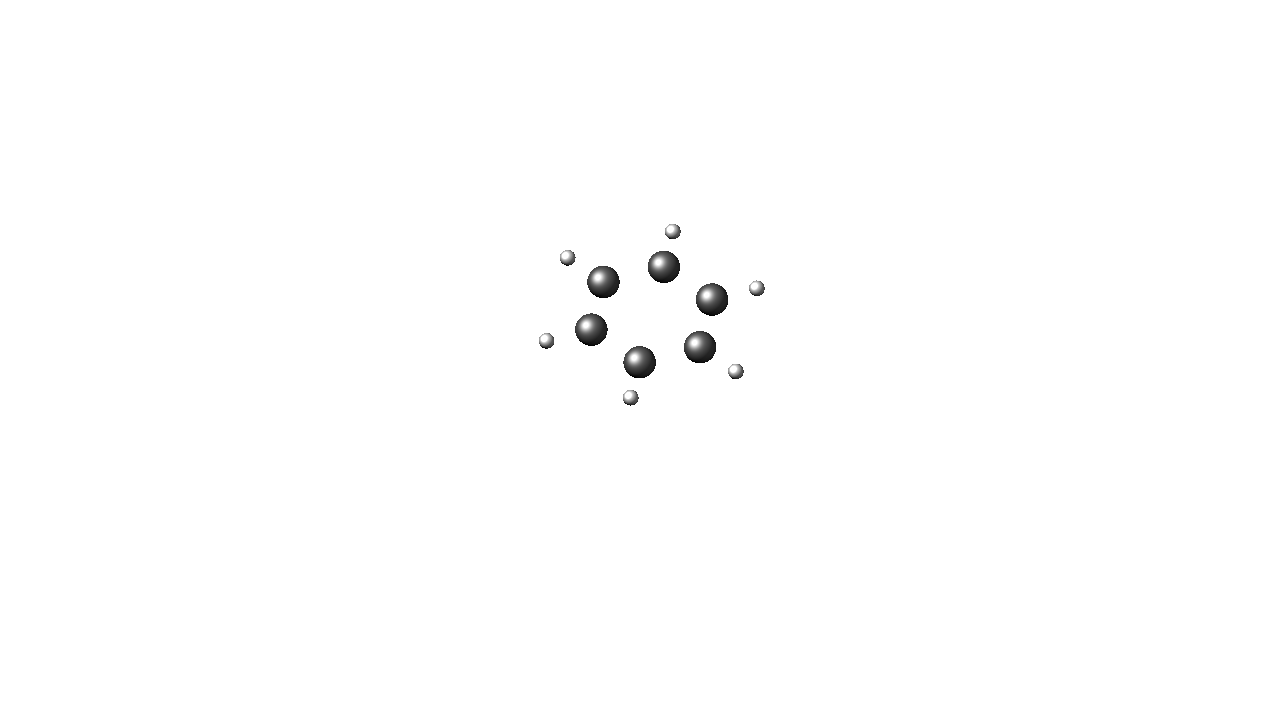
\includegraphics[width=0.40\textwidth]{c06h06}
    \bicaption{\enspace 样图}{\enspace Sample Figure}
    \fignote{对图片的注释}
    \label{fig:c06h06}

\end{figure}

如果插图的空白区域过大,以图片\verb|c06h06|为例,自动裁剪如图~\ref{fig:c06h06_trim}。
\begin{figure}[!htbp]
    \centering
    %trim option's parameter order: left bottom right top
    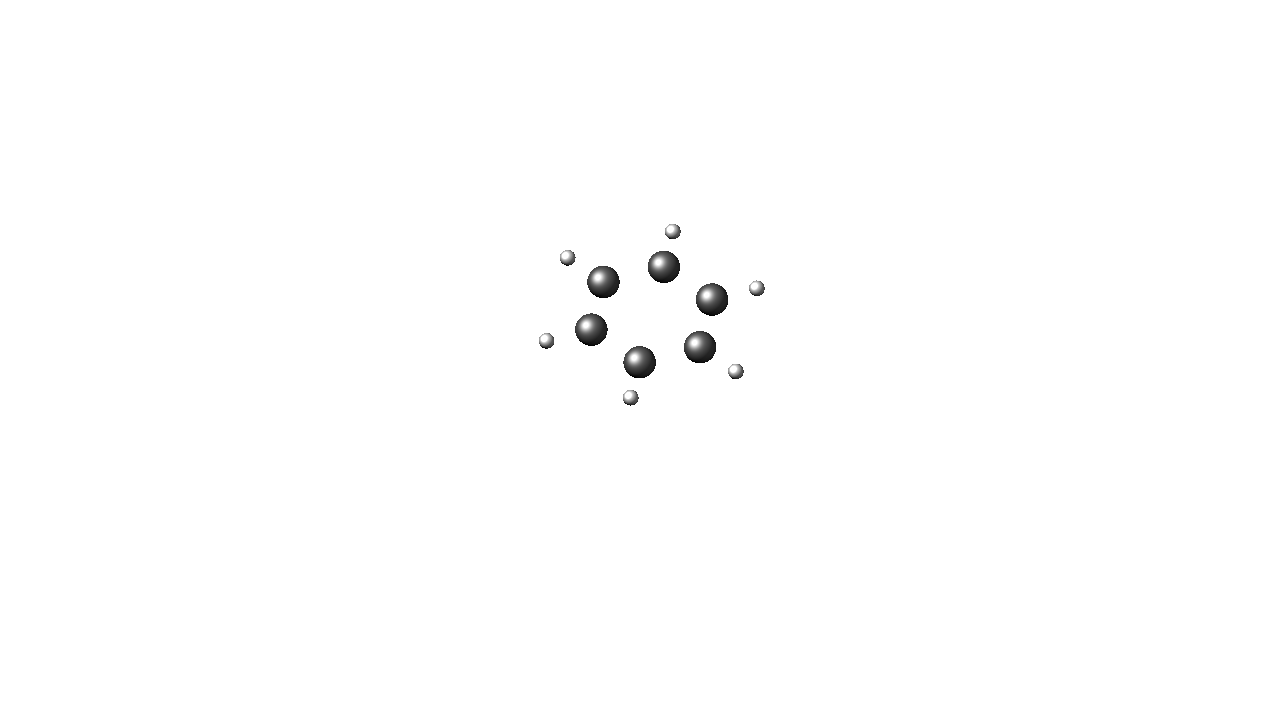
\includegraphics[trim = 60mm 80mm 60mm 60mm, clip, width=0.40\textwidth]{c06h06}
    \bicaption{\enspace 自动裁切测试}{\enspace Auto-Crop Test}
    \label{fig:c06h06_trim}
\end{figure}

多图的插入如图~\ref{fig:oaspl},多图不应在子图中给文本子标题,只要给序号,并在主标题中进行引用说明。
\begin{figure}[!htbp]
    \centering
    \begin{subfigure}[b]{0.35\textwidth}
      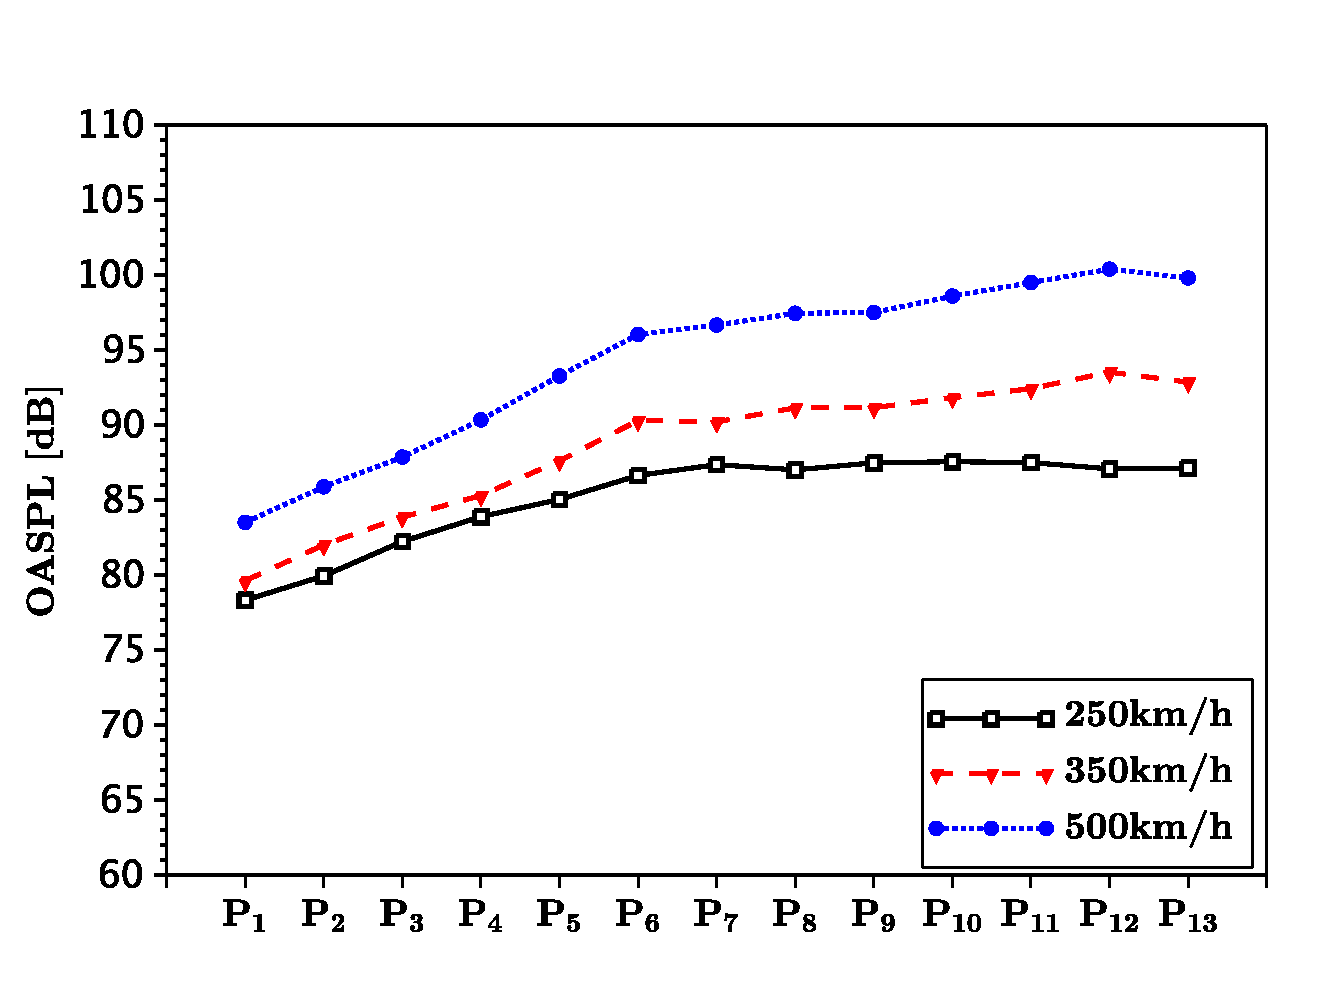
\includegraphics[width=\textwidth]{oaspl_a}
      \caption{}
      \label{fig:oaspl_a}
    \end{subfigure}%
    ~% add desired spacing
    \begin{subfigure}[b]{0.35\textwidth}
      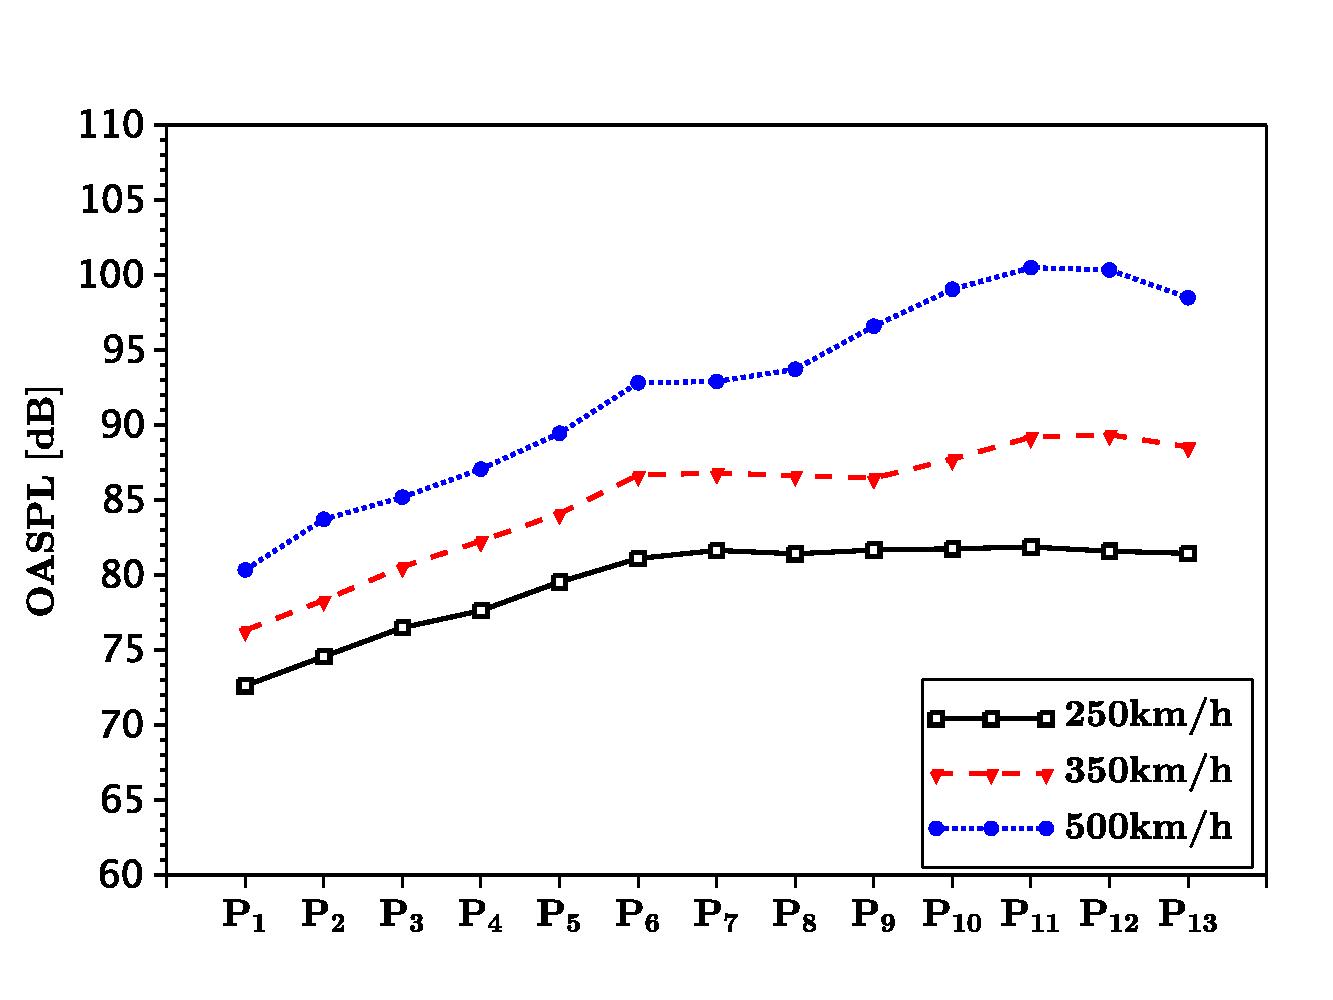
\includegraphics[width=\textwidth]{oaspl_b}
      \caption{}
      \label{fig:oaspl_b}
    \end{subfigure}
    \\% line break
    \begin{subfigure}[b]{0.35\textwidth}
      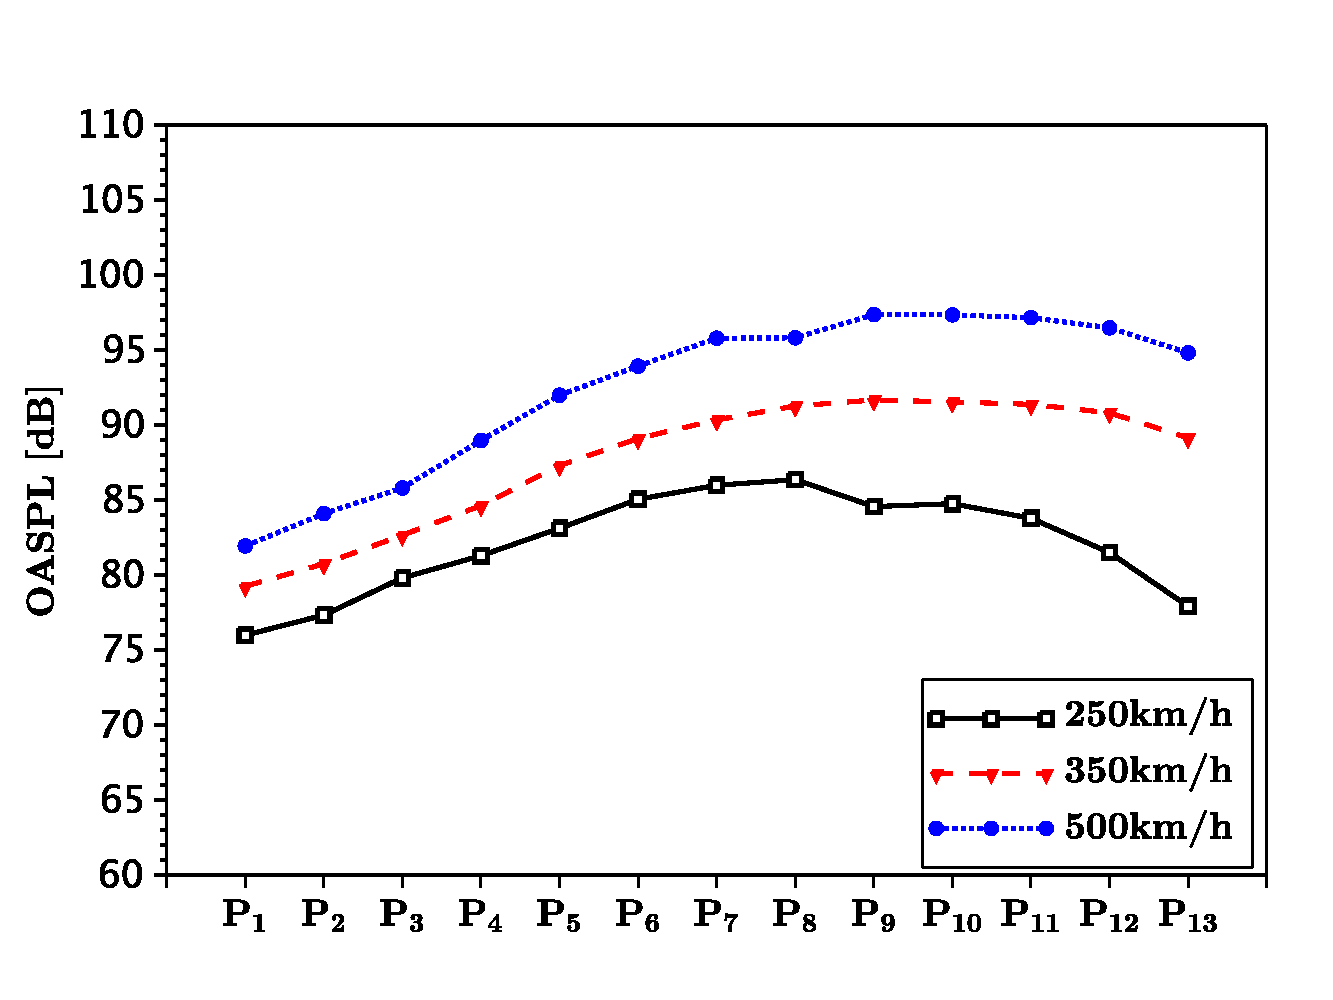
\includegraphics[width=\textwidth]{oaspl_c}
      \caption{}
      \label{fig:oaspl_c}
    \end{subfigure}%
    ~% add desired spacing
    \begin{subfigure}[b]{0.35\textwidth}
      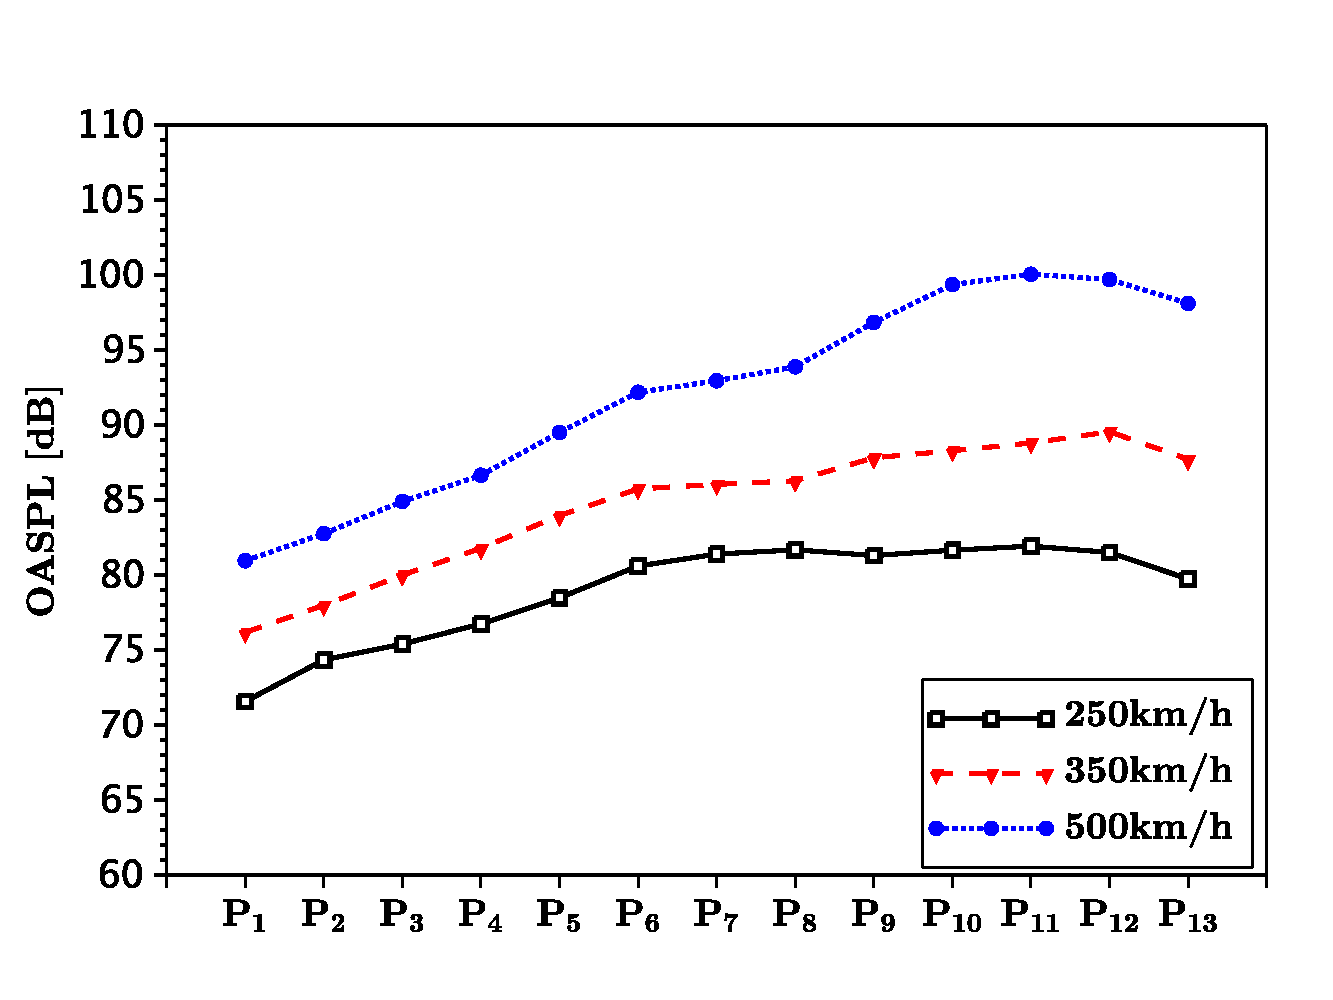
\includegraphics[width=\textwidth]{oaspl_d}
      \caption{}
      \label{fig:oaspl_d}
    \end{subfigure}
    \bicaption{\enspace 多子图测试}{\enspace A test for multi-subfig}
    \label{fig:oaspl}
\end{figure}

\subsection{表}

请见表~\ref{tab:sample}。
\begin{table}[!htbp]
    \bicaption{\enspace 这是一个样表}{\enspace This is a sample table}
    \label{tab:sample}
    \centering
    \footnotesize% fontsize
    \setlength{\tabcolsep}{4pt}% column separation
    \renewcommand{\arraystretch}{1.2}%row space 
    \begin{tabular}{lcccccccc}
        \hline
        行号 & \multicolumn{8}{c}{跨多列的标题}\\
        %\cline{2-9}% partial hline from column i to column j
        \hline
        Row 1 & $1$ & $2$ & $3$ & $4$ & $5$ & $6$ & $7$ & $8$\\
        Row 2 & $1$ & $2$ & $3$ & $4$ & $5$ & $6$ & $7$ & $8$\\
        Row 3 & $1$ & $2$ & $3$ & $4$ & $5$ & $6$ & $7$ & $8$\\
        Row 4 & $1$ & $2$ & $3$ & $4$ & $5$ & $6$ & $7$ & $8$\\
        \hline
    \end{tabular}
\end{table}

制图制表的更多范例,请见 \href{https://github.com/mohuangrui/ucasthesis/wiki}{ucasthesis 知识小站} 和 \href{https://en.wikibooks.org/wiki/LaTeX/Tables}{WiKibook Tables}。

\subsection{参考文献引用}

参考文献引用过程以实例进行介绍,假设需要引用名为"Document Preparation System"的文献,步骤如下:

1)将Bib格式的参考文献信息添加到ref.bib文件中(此文件位于Biblio文件夹下),如直接粘贴自网站,请注意修改其格式。

2)索引第一行 \verb|@article{lamport1986document,|中 \verb|lamport1986document| 即为此文献的label (中文文献也必须使用英文label,一般遵照:姓氏拼音+年份+标题第一字拼音的格式),想要在论文中索引此文献,\verb|\citep{lamport1986document}|。如此处所示 \citep{lamport1986document}。

多文献索引用英文逗号隔开, 如此处所示 \citep{lamport1986document, chu2004tushu, chen2005zhulu}。

更多例子如:

Walls等\citep{walls2013drought}根据Betts\citep{betts2005aging} 的研究,首次提出......理论。其中关于......的研究\citep{walls2013drought, betts2005aging},是当前中国得到迅速发展的研究领域 \citep{chen1980zhongguo, bravo1990comparative}。

不同文献样式和引用样式,如著者-出版年制(authoryear)、顺序编码制(numbers)、上标顺序编码制(super)可在Thesis.tex中对artratex.sty调用实现,详见 \href{https://github.com/mohuangrui/ucasthesis/wiki}{ucasthesis 知识小站之文献样式}。

%若在上标顺序编码制(super)模式下,希望在特定位置将上标改为嵌入式标,可使用 \citetns{niu2013zonghe,stamerjohanns2009mathml} 和 \citepns{niu2013zonghe,stamerjohanns2009mathml}。

参考文献索引的更多知识,请见 \href{https://en.wikibooks.org/wiki/LaTeX/Bibliography_Management}{WiKibook Bibliography}。\nocite{*}% 使文献列表显示所有参考文献(包括未引用文献)

\section{常见使用问题}\label{sec:qa}

设置文档样式: 在artratex.sty中搜索关键字定位相应命令,然后修改
\begin{enumerate}
    \item 正文行距:启用和设置 \verb|\linespread{1.25}|,默认1.25倍行距。
    \item 参考文献行距:修改 \verb|\setlength{\bibsep}{0.0ex}|
    \item 目录显示级数:修改 \verb|\setcounter{tocdepth}{2}|
    \item 文档超链接的颜色及其显示:修改 \verb|\hypersetup|
\end{enumerate}

文档内字体切换方法:
    \begin{itemize}
        \item 宋体:国科大论文模板ucasthesis 或 \textrm{国科大论文模板ucasthesis}
        \item 粗宋体:{\bfseries 国科大论文模板ucasthesis} 或 \textbf{国科大论文模板ucasthesis}
        \item 黑体:{\sffamily 国科大论文模板ucasthesis} 或 \textsf{国科大论文模板ucasthesis}
        \item 粗黑体:{\bfseries\sffamily 国科大论文模板ucasthesis} 或 \textsf{\bfseries 国科大论文模板ucasthesis}
        \item 仿宋:{\ttfamily 国科大论文模板ucasthesis} 或 \texttt{国科大论文模板ucasthesis}
        \item 粗仿宋:{\bfseries\ttfamily 国科大论文模板ucasthesis} 或 \texttt{\bfseries 国科大论文模板ucasthesis}
        \item 楷体:{\itshape 国科大论文模板ucasthesis} 或 \textit{国科大论文模板ucasthesis}
        \item 粗楷体:{\bfseries\itshape 国科大论文模板ucasthesis} 或 \textit{\bfseries 国科大论文模板ucasthesis}
    \end{itemize}
    
对附录的引用,如对附录\ref{chap:app1}的引用。
对附录中图表的引用,如,对附表\ref{apptab:1}的引用。
\let\cleardoublepage\relax
}

%\chapter{中国科学院大学
研究生学位论文撰写规范指导意见(节选)}{
{
\let\cleardoublepage\relax
}
学位论文是研究生在掌握已有的科学知识的基础上,运用科学思维和一定的科学方法、技术与工具,面向特定的科学领域所存在的科学问题,开展创新性研究而产生的科学研究成果。

学位论文是研究生科研工作成果的集中体现,是评判学位申请者学术水平、授予其学位的主要依据,是科研领域重要的文献资料。撰写学位论文是对研究生科学研究能力的基本训练,是研究生学业与研究成效的基本检验,也是科研与创新能力的重要体现。

为提高研究生学位论文的撰写质量,促进学位论文在内容和格式上的规范化,参照《学位论文编写规则》(GB/T 7713.1—2006)、《信息与文献 参考文献著录规则》(GB/T 7714—2015)和《学术出版规范 期刊学术不端行为界定》(CY/T 174—2019)等国家有关标准,特制定本指导意见(2021年修订)。各学科群学位评定分委员会(以下简称各学科群分会)可结合本学科领域的特点,参考本指导意见,制订符合本学科领域特点与要求的学位论文撰写具体要求。

本指导意见从2023年冬季批次开始实施。

\section{组成及要求}
学位论文一般由以下几个部分组成:封面、原创性声明及授权使用声明、摘要、目录、符号说明(若有)、正文、参考文献、附录(若有)、致谢、作者简历及攻读学位期间发表的学术论文与其他相关学术成果等。
\subsection{封面}
一律采用中国科学院大学规定的统一中英文封面,封面包含内容如下:

\begin{enumerate}
    \item 密级,涉密或延迟公开论文必须在论文封面标注密级,同时注明保密年限。公开论文不标注密级,可删除此行。
    \item 论文题目,应简明扼要地概括和反映整个论文的核心内容,一般不宜超过25个汉字(符),英文题目一般不应超过150个字母,必要时可加副标题。题目中应尽量避免使用缩略词、首字母缩写词、字符、代号和公式等。
    \item 作者姓名,根据《中国人名汉语拼音字母拼写规则》(GB/T 28039—2011),英文封面中的姓和名分写,姓在前,名在后,姓名之间用空格分开。姓和名需写全拼,姓全大写,名首字母大写。外国留学生姓名书写顺序以护照格式为准,字母全部大写。
    \item 指导教师,需同时填写导师姓名、专业技术职务和工作单位。如果有多位导师(均需经培养单位批准,并在学籍系统备案),第一导师在前,第二导师等依次在后。学位论文在指导小组的指导下完成的,应注明指导小组成员相应信息。
    \item 学位类别,包括学科门类(学术型)或专业学位类别以及学位级别。学科门类如理学、医学等,专业学位类别如应用统计、工商管理等。学位级别包括硕士、博士。
    \item 学科专业,填写攻读学位的一级学科/二级学科或专业学位类别/领域全称,须与学籍信息一致,不可用简写。
    \item 培养单位,填写就读研究所或学院、系全称,如中国科学院××研究所、中国科学院大学××学院。
    \item 时间,填写论文提交学位授予单位的年月,使用阿拉伯数字标注。一般夏季申请学位的论文标注6月,冬季申请学位的论文标注12月。例如:2023年6月,2023年12月。
\end{enumerate}

\subsection{原创性声明及授权使用声明}
本部分内容提供统一的模版,提交时作者和导师须亲笔签名。如遇导师无法签字时,培养单位应做出适当处理。
\subsection{摘要和关键词}
论文摘要包括中文摘要和英文摘要(Abstract)两部分。论文摘要应概括地反映出本论文的主要内容,说明本论文的主要研究目的、内容、方法、结论。要突出本论文的创造性成果或新见解,不宜使用公式、图表、表格或其他插图材料,不标注引用文献。中文摘要的字数由各学科群分会根据本分会涉及学科专业的特点提出具体要求。英文摘要与中文摘要内容应保持一致。留学生用其他语种撰写学位论文时,应有详细的中文摘要,字数由各学科群分会具体制定,建议一般不少于5000字。

摘要最后注明本文的关键词(3~5个)。关键词是为了文献标引和检索工作,从论文中选取出来,用以表示全文主题内容信息的单词或术语。关键词以显著的字符另起一行并隔行排列于摘要下方,左顶格,中文关键词间用中文逗号隔开。英文关键词应与中文关键词对应,首字母应大写,用英文逗号隔开。

摘要应另起一页,与正文前的内容连续编页(用罗马字符)。
\subsection{目录}
目录应包括论文正文中的全部内容的标题,以及参考文献、附录(若有)和致谢等,不包括中英文摘要。目录页由论文的章、条、附录等序号、名称和页码组成。正文章节题名要求最多编到第三级标题,即×.×.×(如1.1.1)。一级标题顶格书写,二级标题缩进一个汉字符位置,三级标题缩进两个汉字符位置。论文中若有图表,应有图表目录,置于目录页之后,另页编排。图表目录应有序号、图题或表题和页码。

目录应另起一页,与正文前的内容连续编页(用罗马字符)。
\subsection{符号说明(若有)}
如果论文中使用了大量的物理量符号、标志、缩略词、专门计量单位、自定义名词和术语等,应编写成注释说明汇集表。若上述符号等使用数量不多,可以不设此部分,但必须在论文中首次出现时加以说明。
论文中若有符号说明,应置于目录之后、正文之前,另起一页,与正文前的内容连续编页(用罗马字符)。
\subsection{正文}
正文一般包括绪论、论文主体、研究结论与展望等部分。

\begin{enumerate}
    \item 绪论应包括选题的背景和意义,国内外相关研究成果与进展述评,本论文所要解决的科学与技术问题、所运用的主要理论和方法、基本思路和论文结构等。绪论应独立成章,用足够的文字叙述,不与摘要雷同。要实事求是,不夸大也不弱化前人的工作和自己的工作。
    \item 论文主体是正文的核心部分,占主要篇幅,它是将学习和研究过程中调查、观察和测试所获得的材料和数据,经过思考判断、加工整理和分析研究,进而形成论点。依据学科专业及具体选题,论文主体可以有不同的表现形式,可以按照章与节的结构表述,也可以按照“研究背景与意义—研究方法与过程—研究结果与讨论”的表述形式组织论文。但主体内容必须实事求是,客观诚实,准确完备,合乎逻辑,层次分明,简明可读。
    \item 研究结论是对整个论文主要成果的总结,不是正文中各章小结的简单重复,应准确、完整、明确、精炼。应明确凝练出本研究的主要创新点,对论文的学术价值和应用价值等加以分析和评价,说明本项研究的局限性或研究中尚难解决的问题,并提出今后进一步在本研究方向进行研究工作的设想或建议。结论部分应严格区分本人研究成果与他人科研成果的界限。
\end{enumerate}
\subsection{参考文献}
本着严谨求实的科学态度撰写论文,凡学位论文中有引用或参考、借鉴他人思想或成果之处,均应按一定的引用规范,列于文末(通篇正文之后),参考文献部分应与正文的文献引用一一对应,注重合理引用,严禁抄袭剽窃等学术不端行为。
\subsection{附录(若有)}
主要列入正文内过分冗长的公式推导、供查读方便所需的辅助性数学工具或表格、数据图表、程序全文及说明、调查问卷、实验说明等。
\subsection{致谢}
对给予各类资助、指导和协助完成研究工作,以及提供各种对论文工作有利条件的单位及个人表示感谢。致谢应实事求是,切忌浮夸与庸俗之词。致谢末尾应具日期,日期与论文封面一致。
\subsection{作者简历及攻读学位期间发表的学术论文与其他相关学术成果}
作者简历应包括从大学起到申请学位时的个人学习工作经历。按学术论文发表的时间顺序,列出作者本人在攻读学位期间发表或已录用的学术论文清单(著录格式同参考文献)。其他相关学术成果可以是申请的专利、获得的奖项及完成的项目等代表本人学术成就的各类成果。


\section{撰写要求}

\subsection{学位论文基本要求}
学位论文必须是一篇系统的、完整的学术论文,遵循既定的学术规范与要求,不仅要符合学位论文的形式规范,更要符合学位论文的质量规范。做到:学术观点明确,立论正确,方法科学,材料翔实,数据可靠,推理严谨,论证充分,引用规范,结构合理,层次分明,文字通顺,表达准确,学风严谨。研究成果体现作者独到的学术见解、科学论证与创新性结论,表明作者掌握了坚实的基础理论和系统的专门知识,具有独立地从事科学研究的能力。

硕士学位论文选题应为本学科重要领域,有一定的理论意义或应用价值;在理论或方法上有一定的创新,解决了科学或生产实践中某一项重要的问题,取得重要的研究成果,具有较好的社会效益或应用前景。

博士学位论文选题应为本学科前沿领域,有重要的理论意义或应用价值;在理论或方法上有较大的创新,解决了科学或生产实践中某一项重大的问题,取得突破性的研究成果,具有重要的社会效益或应用前景。

\subsection{论文原创性要求}

学位论文应为学位申请者在导师的指导下独立完成的科学研究成果,为作者本人的原创性成果,系研究生经过多年的专业学习和科学研究,运用科学思维、科学方法或工具,探索科学领域中的某一科学问题,提出问题,分析问题,解决问题。学位论文中要有清晰完整的文献综述,但不能以文献综述来代替学位论文。论文引用规范合理,没有伪造、篡改、剽窃、他人代写、论文买卖及其它学术不端行为。

\subsection{论文创新性要求}

学位论文的研究既包括创造知识,即创新、发现和发明,是对未知世界及其规律的探索,也包括整理知识,即对已有知识分析整理,使其规范化、系统化,是对已有知识的传承。创新活动,贯穿了学位论文研究与写作的全过程,如提出新的学术思想、科学概念、假说、学说、定理、定律,设计新的观察方法和实验手段,建立新的科学模型,研制出新的产品,设计出新的工艺流程,发现新的物种等。学位论文的价值在于探索未知,发现科学发展中的规律与特征。学位论文要体现其应有的严谨性与探索性,在原创性的基础上实现对已有知识的超越、突破或颠覆,发现前所未有的科学问题,提出前所未有的分析论证,得出前所未有的科学结论。

\subsection{学位论文的字数要求}
学位论文最重要的意义在于其学术研究的创新性,应将学位论文的质量水平作为主要考量,不以字数多少作为特别要求,但各学科群分会可根据本领域涉及的学科专业特点做相应规定。

\subsection{文字、标点符号和数字}

除外国来华留学生、外语专业研究生以及特殊需要外,学位论文一律用国家正式公布实施的简化汉字书写。标点符号的用法以《标点符号用法》(GB/T 15834—2011)为准。数字用法以《出版物上数字用法》(GB/T 15835—2011)为准。

外国来华留学生可用中文或英文撰写学位论文,但应有详细的中英文摘要。外语专业的学位论文应用所学专业相应的语言撰写,摘要应使用中文和所学专业相应的语言对照撰写。

为了便于国际合作与交流,中文学位论文亦可有英文或其他文字的副本。

\subsection{论文正文}

\subsubsection{章节和各章标题}
论文正文须由另页右页(奇数页)开始,用阿拉伯数字连续编码,一直到全文最后。正文内部新章节无须另页右页(奇数页)开始。
    论文可参考“绪论-研究背景与意义-研究方法与过程-研究结果与讨论-研究结论与展望”的结构形式撰写,各主体研究内容可分别单独成为章节并作为章节标题使用。

各章标题中尽量不采用英文缩写词,对必须采用者,应使用本行业的通用缩写词。标题中尽量不使用标点符号。
\subsubsection{序号}
\textbf{标题序号}

论文标题分层设序。层次以少为宜,根据实际需要选择。各层次标题一律用阿拉伯数字连续编号。以三级标题为宜,最多四级。若确需要再增加一级,以小括号形式表示;不同层次的数字之间用小圆点“.”相隔,末位数字后面不加点号,如“1.1”,“1.1.1”等;章的标题居中排版,各层次的序号均左起顶格排,序号与题名间空一个汉字符。

\textbf{图表等编号}

论文中的图、表、附注、公式、算式等,一律用阿拉伯数字分章依序连续编码。其标注形式应便于互相区别,如:图1-1(第1章第一个图)、图2-2(第2章第二个图);表3-2(第3章第二个表)等。附录的图表参考正文的编号方式,如附图1-1或附表1-1。

\textbf{页码}

正文页码从绪论开始按阿拉伯数字(1,2,3……)连续编排,页码应位居左页左下角、右页右下角;正文前的部分(中英文摘要、目录等)用大写罗马数字(I,II,III…)单独编排,页码位于页面下方居中。
\subsubsection{页眉}
页眉从摘要开始,奇数页上标明“摘要”、“Abstract”、“目录”、“图表目录”等,偶数页上标明论文题目(英文摘要标明英文题目)。正文(即第1章开始到最后一章)的页眉,奇数页上标明每一章名称,偶数页上标明论文题目。参考文献、附录、致谢等的页眉,奇数页标明“参考文献”、“附录”、“致谢”等,偶数页标明论文题目。页眉居中设置。

\subsubsection{名词和术语}
科技名词术语及设备、元件的名称,应采用全国科学技术名词审定委员会公布的权威标准或其他相关权威信息源规定的术语或名称。标准中未规定的术语要采用行业通用术语或名称。全文名词术语必须统一。一些特殊名词或新名词应在适当位置加以说明或注解。双名法的生物学名部分均为拉丁文,并为斜体字。

采用英语缩写词时,除本行业广泛应用的通用缩写词外,文中第一次出现的缩写词应该用括号注明英文原词。新的外来名词应用括号注明英语全称和缩写语。

\subsubsection{量和单位}

量和单位要严格执行《国际单位制及其应用》(GB 3100-93)、《有关量、单位和符号的一般原则》(GB3101—93)有关量和单位的规定。量的符号一般为单个拉丁字母或希腊字母,并一律采用斜体(pH例外)。

\subsubsection{图和表}

论文中若有图和表,应设置图表目录,先列图后列表,置于目录页后,另页编排。

\textbf{(1) 图}

图片大小适当,图边界在页面范围内(图边界离页面边界距离大于页边距)。若图片中包含文字,文字大小不超过正文文字大小。
图包括曲线图、构造图、示意图、框图、流程图、记录图、地图、照片等,宜插入正文适当位置。引用的图必须注明来源。具体要求如下
\begin{itemize}
    \item 图应具有“自明性”,即只看图、图题和图注,不阅读正文,就可理解图意。每一图应有简短确切的图题,连同图序置于图下居中。
    \item 图中的符号标记、代码及实验条件等,可用最简练的文字横排于图框内或图框外的某一部位作为图注说明,全文统一。图题建议用中文及英文两种文字表达。
    \item 照片图要求主要显示部分的轮廓鲜明,便于制版,如用放大、缩小的复制品,必须清晰,反差适中,照片上应有表示目的物尺寸的标尺。
    \item 图片一般设为高6cm×宽8cm,但高、宽也可根据图片量及排版需要按比例缩放。中文(宋体)英文(Times New Roman)图注为五号字,1.25倍行距。
    \item 文中尽量不用世界地图、全国地图!如果一定要用,凡涉国界图件(国内部分地区、全国、世界部分地区、全球)必须使用自然资源部标准地图底图(下载网址:http://bzdt.ch.mnr.gov.cn),所用底图边界要完全无修改(包括南海诸岛位置),为适应排版时图的缩放,比例尺一律用线段比例尺,而不用数字比例尺。并在图题下注明“注:该图基于自然资源部标准地图服务网站下载的审图号为GS(2021)××××号的标准地图制作,底图边界无修改。”
\end{itemize}


\textbf{(2) 表}

表的编排一般是内容和测试项目由左至右横读,数据依序竖排,应有自明性,引用的表必须注明来源。具体要求如下:
\begin{itemize}
    \item 每一表应有简短确切的题名,连同表序置于表上居中。必要时,应将表中的符号、标记、代码及需说明的事项,以最简练的文字横排于表下作为表注。表题建议用中文及英文两种文字表达。
    \item 表内同一栏数字必须上下对齐。表内不应用“同上”、“同左”等类似词及“″”符号,一律填入具体数字或文字,表内“空白”代表无此项,“—”或“…”(因“—”可能与代表阴性反应相混)代表未发现,“0”该表实测结果为零。表内未测出值可以用“N.D. ”表示。
    \item 表格尽量用“三线表”,避免出现竖线,避免使用过大的表格,确有必要时可采用卧排表,正确方位应为“顶左底右”,即表顶朝左,表底朝右。表格太大需要转页时,需要在续表表头上方注明“续表”,表头也应重复排出。
    \item 中文(宋体)英文(Times New Roman)表注为五号字,1.25倍行距。
\end{itemize}

\subsubsection{表达式}
论文中的表达式需另行起,原则上应居中。若有两个以上的表达式,应从“1”开始的阿拉伯数字进行编号,并将编号置于括号内。编号采用右端对齐。表达式较多时可分章编号。

较长的表达式如必须转行,只能在+,-,×,÷,<,>等运算符之后转行,序号编于最后一行右顶格。

\subsection{参考文献}
参考文献格式规范参照《信息与文献 参考文献著录规则》(GB/T 7714—2015),或可参照国际刊物通行的参考文献格式。各学科群分会可根据本学科的一般规范制定相应的参考文献格式。文后参考文献和参考文献在正文中的标注方式可采用“顺序编码制”或“著者—出版年制”。确定采用某种方法后,文后参考文献和参考文献在正文中的标注方式要对应。

文后参考文献按“顺序编码制”组织时,各篇文献应按正文部分首次引用时标注的序号依次列出;文后参考文献按“著者—出版年制”组织时,条目不排序号,先按语种分类排列,语种顺序是:中文、日文、西文、俄文、其他文种;然后按著者字序和出版年排列。中文和日文按第一著者的姓氏笔画排序,中文也可按汉语拼音字母顺序排列,西文和俄文按第一著者姓氏字母顺序排列。当一个著者有多篇文献并为第一著者时,该著者单独署名的文献排在前面(并按出版年份的先后排列),接着排该著者与其他人合写的文献。
文后参考文献加标题“参考文献”,并列入全文目录。
凡正文里标注了参考文献的,其文献都必须列入文后参考文献。文后参考文献应集中著录于正文之后,不分章节著录。
正文中未被引用但被阅读或具有补充信息的文献可集中列入附录中,其标题为“荐读书目”。

详细内容请参考《中国科学院大学研究生学位论文撰写规范指导意见》。

\section{排版与印刷要求}

\subsection{纸张与页面要求}
\begin{table}[h]
    \centering
        \bicaption{\enspace 排版和印刷要求}{\enspace Typography and Printing Requirements}
    \begin{tabular}{lc}
        \hline
        %\multicolumn{num_of_cols_to_merge}{alignment}{contents} \\
        %\cline{i-j}% partial hline from column i to column j
        项目名称 & 要求\\
        \hline
        纸张&A4(210mm×297mm),幅面白色\\
        页面设置&上、下2.54cm,左、右3.17cm,页眉、页脚距页边界1.5cm\\
        封面&采用国科大统一格式\\
        页眉&宋体小五号居中,英文和阿拉伯数字用Times New Roman体\\
        页码&Times New Roman体小五号 \\

        \hline
    \end{tabular}

    \label{tab:printrequirements}
\end{table}

\subsection{印刷及装订要求}
论文封面使用中国科学院大学统一的封面格式。学位论文用A4标准纸(210 mm×297 mm)打印、印刷或复印,按顺序装订成册。自中文摘要起双面印刷,之前部分单面印刷。中文摘要、英文摘要、目录、论文正文、参考文献、附录、致谢、作者简历及攻读学位期间发表的学术论文与其他相关学术成果等,均须由另页右页(奇数页)开始。论文必须用线装或热胶装订,不使用钉子装订。封面用纸一般为150克花纹纸(需保证论文封面印刷质量,字迹清晰、不脱落),博士学位论文封面颜色为红色,硕士学位论文封面颜色为蓝色。

\subsection{书脊}
学位论文的书脊用黑体,英文和阿拉伯数字用Times New Roman体,字号一般为小四号,可根据论文厚度适当调整。上方写论文题目,中间写作者姓名,下方写“中国科学院大学”,距上下边界均为3cm左右。}
%---------------------------------------------------------------------------%
